%%%%%%%%%%%%%%%%%%%%%%%%%%%%%%%%%%%%%%%%%%%%%%%%%%%%%%%%%%%%%%%
%% OXFORD THESIS TEMPLATE

% Originally by Keith A. Gillow (gillow@maths.ox.ac.uk), 1997
% Modified by Sam Evans (sam@samuelevansresearch.org), 2007
% Modified by John McManigle (john@oxfordechoes.com), 2015
% Modified by Maud Gautier (https://github.com/MaudGautier), 2019
% Modified by Thibault Latrille (https://github.com/ThibaultLatrille), 2020
% Modified by Alexandre Laverré (alex.laverre@gmail.com), 2022
%
% This version Copyright (c) 2020 Thibault Latrille
%
% Broad permissions are granted to use, modify, and distribute this software
% as specified in the MIT License included in this distribution's LICENSE file.

%%%%% CHOOSE PAGE LAYOUT
\documentclass[a4paper,openright,twoside, nobind]{thesis}
\usepackage{textgreek}
\usepackage[unicode]{hyperref}
\usepackage{amsmath}
\usepackage{bm}
\usepackage{bbm}
\definecolor{Nonpolar}{HTML}{fef1d2}
\definecolor{Polar}{HTML}{a9fdd8}
\definecolor{Basic}{HTML}{d7f8ff}
\definecolor{Acidic}{HTML}{feceea}
\definecolor{Stop}{HTML}{D0D0D0}
\graphicspath{{figures/}{figures/introduction}}
\makeatletter
\makeatother

%%%%% Glossary
\usepackage[toc, acronym]{glossaries}
\renewcommand*{\glstextformat}[1]{\textcolor{black}{#1}}
\makeglossaries

%%%% FlipBook
\usepackage{flipbook}
\newcommand{\initflipbook}{
\fancyfoot[RO]{                           % Flipbook at right foot in odd pages
\setlength\unitlength{1cm}                % Specify the units
  \begin{picture}(0,0)                    % New picture
    \put(-1.7,-1.0){                        % Position of the picture
      \fbImageF{figures/flipbook/slide}{png}{width=4cm} % Insert numbered picture in increasing order. Directory: ./Fig/Flipbook. Prefix of all pictures: image_ (in fact image_1, image_2, ...). Extension of the pictures: png. 
     }
 \end{picture}
}
\fancyfoot[LE]{                           % Flipbook at left foot in odd pages
\setlength\unitlength{1cm}                % Specify the units
  \begin{picture}(0,0)                    % New picture
    \put(-3,-1){                        % Position of the picture
      \fbImageF{figures/flipbook/slide}{png}{width=4cm} % Insert numbered picture in increasing order. Directory: ./Fig/Flipbook. Prefix of all pictures: image_ (in fact image_1, image_2, ...). Extension of the pictures: png. 
     }
 \end{picture}
}
}

%%%%% Initialize glossaries before begin
\newacronym{3C}{3C}{Capture de la Conformation des Chromosomes}
\newacronym{ADN}{ADN}{Acide Désoxyribo-Nucléique}
\newacronym{ARN}{ARN}{Acide Ribo-Nucléique}
\newacronym{ARNm}{ARNm}{Acide Ribo-Nucléique messager}
\newacronym{CAGE}{CAGE}{Cap Analysis of Gene Expression}
\newacronym{ChIP-seq}{ChIP-seq}{Chromatin Immuno-Precipitation sequencing ou séquençage par Immunoprécipitation de la Chromatine}
\newacronym{CpG}{CpG}{Cytosine–phosphate-Guanine ou dinucléotide Cytosine-Guanine}
\newacronym{CTCF}{CTCF}{Facteur de transcription se fixant au motif CCCTC}
\newacronym{eRNA}{eRNA}{enhancer Ribo-Nucléique Acid ou Acide Ribo-Nucléique produit par les éléments amplificateurs de l'expression}
\newacronym{FT}{FT}{Facteur de Transcription}
\newacronym{GFP}{GFP}{Green Fluorescent Protein ou protéine fluorescente verte}
\newacronym{Hi-C}{Hi-C}{High-throughput technique to capture chromatin conformation}
\newacronym{PCHi-C}{PCHi-C}{Promoter Capture Hi-C}
\newacronym{PCR}{PCR}{Polymerase Chain Reaction}
\newacronym{RNA-seq}{RNA-seq}{Ribo-Nucléique Acid sequencing ou séquençage des Acides Ribo-Nucléiques}
\newacronym{RPKM}{RPKM}{Read Per Kilobase per Million ou lecture de séquençage par kilobase par million}
\newacronym{SHH}{SHH}{Sonic HedgeHog}
\newacronym{TAD}{TAD}{Topological Associated Domain ou domaine d'association topologique}
\newacronym{TSS}{TSS}{site d'initiation de la transcription}
\newacronym{ZRS}{ZRS}{Zone of polarising activity Regulatory Sequence ou séquence régulatrice de l'activité de la zone polarisante}


\newglossaryentry{cis}{name={\textit{cis}},description={séquence d'ADN ou mécanisme de régulation dont les gènes cibles sont situés sur le même chromosome.}}

\newglossaryentry{trans}{name={\textit{trans}},description={séquence d’ADN ou mécanisme de régulation agissant par le biais de produits (protéines ou ARNs) qui circulent dans le noyau des cellules et dont les gènes cibles ne sont pas nécessairement situés sur le même chromosome.}}

\newglossaryentry{amplificateur}{
name={amplificateur}, plural={amplificateurs},
description={élément \textit{cis}-régulateur de l'expression d'un gène dont l'activité participe à l'initiation et/ou l'amplification de la transcription}}
  
\newglossaryentry{condition}{name={condition biologique}, plural={conditions}, description={décrit l'état d'une cellule, peut refèrer à des types cellulaires, tissus ou organes distincts, des stades du développement, ou un environnement biochimique}}

%\printglossary[type=\acronymtype]
%\printglossary

%\mtcaddchapter
%\mtcaddchapter

%%%%% THE ACTUAL DOCUMENT STARTS HERE
\begin{document}

%%% hyphenation rules
\hyphenation{d\'e-ve-lop-pe-ment}
\hyphenation{d\'e-ve-lop-p\'es}
\hyphenation{d\'e-ve-lop-p\'ees}
\hyphenation{d\'e-ve-lop-pementaux}
\hyphenation{am-pli-fi-ca-teurs}
\hyphenation{am-pli-fi-ca-teur}
\hyphenation{d'am-pli-fi-ca-teur}
\hyphenation{d'am-pli-fi-ca-teurs}

%mini-toc in french:
\mtcselectlanguage{french} 
\initflipbook
    \pagenumbering{gobble}
    \hypersetup{pageanchor=false}
    \thispagestyle{empty}
\vspace*{\stretch{1}}

\unitlength 1cm
\begin{center}
    \vspace*{-2.5cm}
    \begin{figure}[h]
        \centering
        
\includegraphics[width=0.8\textwidth]{figures/Logo_Lyon_UCBL.jpg}
    \end{figure}

    {\large \textbf{THÈSE de DOCTORAT DE L'UNIVERSITÉ DE LYON}\\}
    {Opérée au sein de~:\\}
    {\large \textbf{l'Université Claude Bernard Lyon 1}\\}
    \vspace{12pt}
    {\large \textbf{Ecole Doctorale} 341 \\
    \vspace{0.15cm}
    Écosystèmes Évolution Modélisation Microbiologie
    }
    
    \vspace{12pt}
    {\large \textbf{Spécialité de doctorat~:} Génomique évolutive
    \\}
    \vspace{0.8cm}

    {Soutenue publiquement le 13/07/2022, par~:\\}
    \vspace{0.15cm}
    {\Large \textbf{Alexandre Laverré}\\}
    \vspace{0.5cm}
    \rule{5cm}{1pt}
    
    \vspace{12pt}
    {\Large \textbf{Relations entre l’évolution des paysages cis-régulateurs, l’évolution de l’expression des gènes et l’évolution phénotypique chez les vertébrés}\par}
    \vspace{12pt}
    \rule{5cm}{1pt}
    \vspace{0.5cm}

\end{center}

\large{Devant le jury composé de~:\\\\}
\small {
\renewcommand{\arraystretch}{1.2}
\begin{tabular}{ll}
    \textbf{Cristina VIEIRA} &  \textbf{Présidente}         \\
    Professeure, Université Claude Bernard Lyon 1 \\
    
    \textbf{Mélanie DEBIAIS-THIBAUD} & \textbf{Rapportrice}         \\
    Maîtresse de conférences, Université de Montpellier \\
    
    \textbf{Hugues ROEST-CROLLIUS} & \textbf{Rapporteur}         \\
    Directeur de recherche CNRS, Institut de Biologie de l'ENS             \\
    
    \textbf{Camille BERTHELOT}  & \textbf{Examinatrice}        \\
    Chargée de recherche INSERM, Institut Pasteur \\
    
    \textbf{Anamaria NECSULEA}       & \textbf{Directrice de thèse} \\
    Chargée de recherche CNRS, LBBE \\
    
    \textbf{Éric TANNIER}       & \textbf{Co-directeur de thèse} \\
    Directeur de de recherche INRIA, LBBE \\
\end{tabular}
}
\vspace*{\stretch{3}}

    
%%%%% CHOOSE YOUR LINE SPACING HERE
    \setlength{\textbaselineskip}{2em}
% You can set the spacing here for the roman-numbered pages (acknowledgements, table of contents, etc.)
    \setlength{\frontmatterbaselineskip}{1em}
% Leave this line alone; it gets things started for the real document.
    \setlength{\baselineskip}{\textbaselineskip}

%%%%% CHOOSE YOUR SECTION NUMBERING DEPTH HERE
% The level that gets a number:
    \setcounter{secnumdepth}{2}
% The level that shows up in the ToC:
    \setcounter{tocdepth}{3}
    \setcounter{minitocdepth}{3}

%%%%% ABSTRACT
    \setlength{\baselineskip}{1.5\frontmatterbaselineskip}
    \begin{alwayssingle}
        \input{parts/2_resumé}
    \end{alwayssingle}

%%%%% ACKNOWLEDGEMENTS
    \begin{alwayssingle}
    	\chapter*{Remerciements}
\label{remerciements}

Je souhaite remercier tout d’abord Camille Berthelot, Mélanie Debiais-Thibaud, Hugues Roest-Crollius et Cristina Vieira d’avoir accepté d’évaluer mes travaux de thèse.\\

Je voudrais également remercier les personnes qui ont participé à mes trois comités de suivi de thèse Yad Ghavi-Helm, Franck Picard, Dominique Mouchiroud, ma tutrice Clémentine François et encore une fois Camille Berthelot pour votre écoute, vos conseils avisés et votre bienveillance.\\

Je n'aurais jamais pu faire cette thèse sans mes superbes encadrant.e.s Anouk et Eric. Merci à vous deux de m'avoir proposé ce stage et de m'avoir suivi avec bienveillance ces quatres dernières années. Anouk, merci infiniment d'avoir cru en moi depuis le tout début et d'avoir eu cette envie de m'accompagner pour une thèse. J'ai tellement appris avec toi, je n'aurais jamais pu rêver d'un meilleur encadrement. Merci pour ta disponibilité, ta patience et ta gentillesse. Comme dirait Théo, tu es maintenant ma maman de la Science. \\

Je tiens ensuite à remercier tous les membres de mon équipe de bioinformatique, phylogénie et génomique évolutive pour leur sagesse et leur contribution majeure à mon ouverture scientifique. Je remercie particulièrement Laurent Duret pour ses conseils toujours pertinents et pour m’avoir permis de franchir les portes du LBBE en faisant circuler mon CV dans le labo quand je cherchais un stage.\\

Je souhaite remercier l’ensemble des personnes avec qui j’ai eu l’occasion de travailler sur différents projets au cours de ma thèse. Merci à Nelly Burlet pour sa disponibilité, ses conseils et pour nous avoir permis d’enfiler une blouse blanche, petit.e.s bio-informaticien.ne.s que nous sommes, dans nos tentatives d’extraction d’ADN de plumes. Merci à Marie Fablet et Timothée Kastylevsky pour leur contribution à l’analyse des éléments répétés des génomes d’oiseaux. Merci à Etienne Rajon, Florian Labourel, Mariana Ferrarini et Sergio Peignier pour cette initiative de recherche sur ACE2 au moment où le monde entier basculait dans un premier confinement. Vous m’avez permis de retrouver un peu de sens dans mon activité de recherche à un moment crucial. Merci beaucoup à Patrick Tschopp et Maëva Luxey de l'université de Bâle pour leur implication sans faille dans l'étude des phallus d'oiseaux et les nombreux échanges toujours très constructifs. \\

Merci également aux personnes qui m'ont permis de décrouvrir le monde de l'enseignement, Véronique Daviero, Frédéric Thévenard, Anne-Kristel Bittebière, Arnaud Mary, et surtout merci à l'ensemble de mes étudiant.e.s qui m'ont donné le goût de transmettre des connaissances. Les TPs à balader dans les serres botaniques pour raconter la vie des plantes vont bien plus me manquer que les TPs de biostats en visio ! \\

Merci à toutes les personnes du pôle informatique du LBBE, particulièrement Bruno Spataro et Stéphane Delmotte que j'ai souvent embêté pour des soucis de cluster, de pbil ou de stockage ! Merci pour le support sans faille et les nombreux conseils que vous apportez à tout ce labo. Merci également à Christophe Blanchet de l'Institut Français de Bio-informatique pour sa gentillesse et pour m'avoir débloqué tous mes problèmes de VM. Merci aussi aux personnes du pôle administratif qui font tourner le labo et nous sauvent dans toutes nos démarches. \\

Merci aux différentes personnes qui ont partagé mon bureau durant ces 4 années, Christine Oger, Philippe Weber, Claire Gayral, Adil El Filali qui ont su animer mon quotidien. Un énorme merci à Alexia, sans qui la vie au labo serait moins fun ! Tu as toujours ce petit grain de folie qui redonne le sourire aux gens. Avec toi on a presque réussi à faire un petit jardin dans ce bureau !\\

Je voudrais aussi remercier l'ensemble des doctorant.e.s, stagiaires, post-doc du LBBE qui ont croisés ma route. Vous êtes la force de ce labo, on se demande comment la science avancerait sans vous, ne l'oubliez pas ! Théo, Djivan, Alexia, on a formé une vraie petite équipe depuis notre arrivée dans ce couloir pour un stage de M2, merci pour tous ces moments. (En fait non, je tiens surtout à ne PAS remercier Théo ;)) Un très grand merci à Thibault Latrille qui a été notre doctorant de référence à tous, qui a toujours trouvé du temps pour répondre à toute nos questions. Je le remercie tout particulièrement pour son template LateX qui m'a occupé la plupart de mes heures ces dernières semaines. Merci à celles et ceux qui sont déjà partis ou qui ont fait des passages trop rapides au LBBE : Pierre, Elise, Maud, Monique, Lucie, Claire, Marina, Diego et j'en oublie sans doute, ne m'en voulez pas! Merci à Mary, Kamal et \'Emilie pour ces instants partagés même dans les plus grand moments de doute dans nos thèses respectives. Merci à toutes les personnes qui mettent de l'ambiance dans ce labo, qui sont toujours partantes pour boire des coups ou faire des pauses café, je pourrai pas citer tout le monde mais merci ! Je souhaite un bon courage aussi à celles et ceux qui sont sur la fin et à la relève : Aissa, Florentin, Chloé, Benjamin, Julien, Laura, Léa, Solène, Lucas, Mélodie et bien d'autres. Pour terminer avec les "non-permanent.e.s", je voudrais vraiment remercier les personnes qui ont partagé l'aventure des Pinsons MigRateurs, au sein du bureau de l'asso, mais aussi de toutes les animations qu'on a pu initier ou pérenniser : week-ends d'inté, séminaires post-thèse, séminaires étudiants, mais aussi les regrettées HappyHours avec nos LBBbières ratées ! Vous avez toute ma confiance pour continuer à faire vivre la vie étudiante (et scientifique) du labo !\\

Merci à tous les gens qui ont partagé mon aventure lyonnaise en dehors du labo. Merci à mes cher.e.s colocs Léa, Eve et Camille avec qui j'ai partagé près de 2 ans de ma vie mais aussi le premier confinement (ça compte triple!). A toutes les belles rencontres que j'ai pu faire : Anaïs, Judith, Camille, Elsa, Romain, Mégane, Coralie, Julia, Clémentine mais aussi toute la Team des Graines électroniques !\\

Merci à tous mes ami.e.s de Montpellier pour le soutien moral et émotionnel, on ne se voit pas assez mais je n'aurais jamais pu tenir sans vous. Un énorme merci à Aurélien et Maurine que j'aime de tout mon coeur. Merci à toute la coloc' de Celleneuve: Maurine, Nathan, Arthur, Taïna, Salma, Léo-Paul, à la coloc' de choc : Aurélien et Thibault, ainsi qu'à Romain pour vraiment tout ce que vous apportez dans ma vie et aussi pour m'avoir toujours accueilli avec plaisir pour une nuit, un week-end (parfois transformée en semaine!) sur Montpellier. J'ai aussi une grosse pensée pour la petite bande du lycée maintenant bien dispersée : Fred, Charlotte, Debora, Gaetan et Julie, vous me manquez ! Merci à tous les copains et les copines que je n'ai pas cités, vous comptez beaucoup !\\

Je voudrais évidemment remercier ma petite famille qui me soutiendra toujours dans tout ce que je fait et dans toutes mes décisions. Maman, Papa, Nath, Nanou, Romain et les petits loups!\\

Finalement, le plus important, merci à mon amoureux, Jordan, qui me rend toujours plus heureux, qui me soutien sans faille depuis 4 ans et qui me donne la force et le courage au quotidien. Merci à toi d'avoir supporté cette thèse autant que moi ! Je t'aime. 




	\end{alwayssingle}
	
%%%%% MINI TABLES
    \hypersetup{pageanchor=true}
    \begin{romanpages}
        \setlength{\baselineskip}{1.5\frontmatterbaselineskip}
        \setlength{\baselineskip}{\frontmatterbaselineskip}
        \dominitoc % include a mini table of contents
%\dominilof  % include a mini list of figures
%\dominilot  % include a mini list of tables
% This aligns the bottom of the text of each page.  It generally makes things look better.
        \flushbottom
% This is where the whole-document ToC appears:
        {\setlength{\baselineskip}{1.1\frontmatterbaselineskip}
        \hypersetup{linkcolor=GREYDARK}
        \tableofcontents
        \listoffigures
        \mtcaddchapter
        %\listoftables
        %\mtcaddchapter
        }
    \end{romanpages}

%%%% Glossaries
\printglossary[type=\acronymtype]
\printglossary
\mtcaddchapter
\mtcaddchapter

%%%%% Avant-propos
    \setlength{\baselineskip}{1.5\frontmatterbaselineskip}
    \begin{alwayssingle}
        \chapter*{Avant-propos}
        % Start page numbering
        \pagenumbering{arabic}
    \end{alwayssingle}
    
%%%% CHAPTERS
    \setlength{\baselineskip}{1.5\frontmatterbaselineskip}
    \flushbottom
    \pagestyle{fancybook}
     % reset flipbook after change of format
    \initflipbook{}

    \part{Introduction}
    \label{part:intro}
    Mes travaux de thèse s'appuient sur des comparaisons de paysages de régulation de l'expression des gènes. Il m’est donc nécessaire de commencer par préciser les notions dont il est question : gènes, expression, régulation, éléments régulateurs, et les techniques de mesure de leur existence ou de leur quantité. Je m’attarderai sur certaines techniques et méthodologies qui ont permis de prédire et mesurer ces objets, avant de contextualiser les connaissances actuelles sur leur évolution et leurs relations, qui ont été le point de départ de ma thèse.

\chapter{L’expression des gènes}
{\hypersetup{linkcolor=GREYDARK}\minitoc}
\label{chap:expression-des-gènes}

\section{Définitions}
\label{sec:definition-des-gènes}

La notion de gène dépend grandement des besoins et des usages qu’on en fait, et sa définition a largement évolué au cours de la compréhension de la complexité moléculaire de l’\acrshort{ADN} \citep{gerstein_what_2007}. D’abord unité de trait héritable \citep{mendel_verhandlungen_1866}, puis région du génome à l’origine d’une protéine \citep{morgan_mechanism_1915,beadle_genetic_1941}, le gène a ensuite été caractérisé comme une séquence précise de l’\acrshort{ADN} \citep{watson_molecular_1953}, qui doit être transcrite puis traduite selon un code génétique pour être fonctionnelle et affecter les caractères d’un organisme \citep{nirenberg_rna_1965}. L’émergence et le développement des techniques de séquençage ont par la suite permis de préciser la structure des gènes en annotant notamment les parties codantes (exons) et non-codantes (promoteur, introns, extrémités), ce qui a rendu possible la prédiction et la détection d’autres catégories de gènes \citep{fiers_complete_1976, doolittle_urfs_1986}. Il est cependant rapidement apparu que l’idée “qu’un gène produit une protéine” était une simplification excessive. Premièrement, la présence de nombreux gènes transcrits en \acrshort{ARN}s directement fonctionnels sans être traduits et ne codant donc pas pour des protéines n'est pas en accord avec une telle idée \citep{lander_initial_2001}. Deuxièmement, le développement de techniques de séquençage à haut débit a révélé la complexité du transcriptome \citep{birney_identification_2007, encode_project_consortium_integrated_2012}. Que ce soit pour les gènes codants pour des protéines ou pour certains gènes non-codants (pour des \acrshort{ARN}s), l’\acrshort{ARN} subit une maturation pour être stabilisé et fonctionnel, notamment un épissage qui consiste à exciser les parties introniques des transcrits pour conserver les exons. Cet épissage peut être variable en retenant certains introns ou en excisant certains exons et peut ainsi produire des transcrits alternatifs pour un même gène. De plus, la transcription d’un gène peut démarrer à partir de sites d’initiation alternatifs engendrant également des transcrits différents. Pour les gènes codants, ces transcrits alternatifs peuvent conduire à différentes versions de protéines appelées isoformes et pouvant avoir des fonctions différentes. La délimitation d’un gène comme unité peut alors être délicate, notamment par le fait que les gènes peuvent se chevaucher et ainsi avoir des parties fonctionnelles en communs. J’utiliserai au cours de cette thèse la définition d’un gène comme étant une séquence d’\acrshort{ADN} qui est transcrite pour produire une molécule pouvant impacter les caractères phénotypiques de l’organisme. \\

Les gènes peuvent produire une quantité variable de produits finaux (protéines ou \acrshort{ARN}s non-codants matures) qui sont potentiellement fonctionnels dans la cellule et plus largement dans l’organisme. Il peut alors être nécessaire de quantifier cette activité, définie comme le niveau d'expression d’un gène, pour estimer son impact. La quantité des produits finaux est cependant difficilement accessible pour de nombreux gènes, notamment ceux codant des protéines. En effet, ces dernières présentent une grande diversité d’abondance mais surtout de structure de par leur constitution en acides aminés et leur conformation tridimensionnelle leur donnant des propriétés biochimiques distinctes. C’est par exemple le cas des protéines trans-membranaires, présentes en très faible quantité et difficilement solubles \citep{vuckovic_membrane_2013}. Les protéines réagissent de manière très diverse aux protocoles expérimentaux et la capture, l’isolation et l’identification de l’ensemble des protéines d’une cellule est très complexe. A ce jour, l’identification des protéines chez humain n’est ainsi toujours pas complétée et nécessite la collaboration de plusieurs centaines d'équipes dans le monde, via le consortium Human Proteome Project, depuis plus de 10 ans \citep{adhikari_high-stringency_2020}. Il est néanmoins possible d’approximer le niveau d’expression d’un gène en mesurant la quantité d’\acrshort{ARN} messager produit lors de sa transcription. Il est en effet plus simple d’isoler et de séquencer l’\acrshort{ARN} messager, composé seulement de quatre nucléotides distincts, que les protéines. Les techniques de séquençage de l’\acrshort{ARN}, dites \acrshort{RNA-seq}, permettent de mesurer la quantité d’\acrshort{ARN}s matures, à l’état stable, et donc après modifications post-transcriptionnelles \citep{chu_rna_2012}. Il a été montré que cette mesure de la quantité d’\acrshort{ARNm} stable d’un gène codant est bien corrélée à la quantité de ses protéines produites dans une cellule \citep{edfors_gene-specific_2016}. L’utilisation du \acrshort{RNA-seq} est aujourd’hui largement répandue et permet de donner une définition plus usuelle du niveau d’expression des gènes comme étant le nombre de molécules d’\acrshort{ARNm} produites par le gène, par cellule, tous transcrits alternatifs confondus. Enfin, un des avantages notables du séquençage d’\acrshort{ARN} est la possibilité d'identifier des nouveaux transcrits et de quantifier l’expression des gènes ne codant pas pour des protéines. \\

Afin d’illustrer mes propos le long de cette introduction, je reviendrai régulièrement sur l’exemple du gène Sonic hedgehog, qui est devenu un modèle pour comprendre les fonctions d’un gène, son expression, sa régulation, mais aussi son évolution. Le gène hedgehog est un gène codant identifié d’abord chez la drosophile pour son rôle crucial dans la segmentation lors du développement embryonnaire \citep{nusslein-volhard_mutations_1980}. Chez les vertébrés ce gène est présent en trois copies, dites homologues, qui ont émergé suite à deux duplications successives du génome complet chez l’ancêtre commun du clade et par la perte d’une copie \citep{dehal_two_2005}. L’expression de ces trois gènes permet notamment de définir la voie de signalisation Hedgehog qui joue plusieurs rôles majeurs lors du développement embryonnaire, comme l’organogénèse, l’organisation du cerveau ou le développement de structures comme les doigts \citep{lum_hedgehog_2004}. L’un de ces homologues les plus étudiés est Sonic hedgehog (\acrshort{SHH}) localisé sur le chromosome 7 chez l’humain. Le niveau d’expression de \acrshort{SHH}, et donc la quantité de la protéine \acrshort{SHH} dans les cellules, permet de définir un gradient de concentration qui va contrôler l’expression de plusieurs autres gènes. Dans le développement des membres par exemple, le gradient de concentration de cette protéine, dans une zone dite de polarisation, est essentiel pour établir un axe antéro-postérieur permettant de définir le nombre et la structure des doigts (Figure \ref{fig:Fig1}) \citep{riddle_sonic_1993, echelard_sonic_1993}.

\begin{figure}[h]
    \centering
    \includegraphics[width=1\textwidth, page=1] {figures/introduction/fig1.png}
    \caption[Schéma de l'impact de l'expression de \acrshort{SHH} au cours du développement d'un membre.]{
    \textbf{Schéma de l'impact de l'expression de \acrshort{SHH} au cours du développement d'un membre.} Le gradient de concentration de la protéine \textit{Shh} dans la zone d'activité polarisante (ZPA) dans le bourgeon du membre permet de définir un axe antéro-postérieur.  Les cellules déterminées par la signalisation SHH
permettront la formation des os postérieurs de l'autopode et du zeugopode.  Tirée de \citep{lezot_shh_2020}
    }
    \label{fig:Fig1}
\end{figure} 


\section{Mesures et comparaisons de l’expression}
\label{sec:mesure-et-comparaison}

L’expression d’un gène varie selon les stades de développement, les types cellulaires ou les facteurs externes. L’expression des gènes est considérée comme le premier échelon du phénotype moléculaire d’un organisme, qu’il est nécessaire de mesurer indépendamment dans chaque échantillon.

\subsection{RNA-seq et niveau d’expression}
\label{subsec:RNAseq-niveau-expression}
Les méthodes de séquençage à haut débit de l’\acrshort{ARN} (\acrshort{RNA-seq}) permettent d’approximer le niveau d’expression des gènes à un instant donné dans un échantillon. Celles-ci s’effectuent généralement sur une population de cellules, ce qui permet d’obtenir une mesure globale d’un ensemble de transcrits produits ou transcriptome. Grâce au développement récent de techniques microfluidiques permettant d’isoler un très faible nombre de cellules, voire des cellules uniques, la quantification du transcriptome peut désormais se faire à l’échelle d’une seule cellule \citep{tang_mrna-seq_2009}. 
 \\

Les techniques de \acrshort{RNA-seq} passent généralement par cinq grandes étapes : l’isolation de l’\acrshort{ARN}, la sélection/déplétion de certains \acrshort{ARN}s, la transcription réverse en \acrshort{ADN} (essentielle à l’étape d’amplification par PCR), l’amplification puis le séquençage à haut débit. L’étape de sélection/déplétion est cruciale car de nombreuses formes distinctes d’\acrshort{ARN} sont présentes dans les cellules. Les \acrshort{ARN}s ribosomaux par exemple, qui sont non codants et permettent la synthèse des protéines, représentent une très grande partie du contenu en \acrshort{ARN} d’une cellule (plus de 80\%) et doivent généralement être filtrés \citep{oneil_ribosomal_2013}. Il est possible de cibler spécifiquement certains types d'\acrshort{ARN}s. Par exemple, les \acrshort{ARN}s messager matures des gènes codants pour des protéines contiennent une séquence terminale poly-A, tout comme certains longs \acrshort{ARN}s non-codants. Ces transcrits peuvent être ciblés en passant par une étape d'hybridation avec des molécules poly-T se liant de manière covalente à la queue poly-A. Il est également possible de viser les petits \acrshort{ARN}s non-codants, tels que les micro\acrshort{ARN}s, piwi\acrshort{ARN}s, etc, en filtrant les transcrits selon leur taille. Certaines techniques dérivées permettent de sélectionner d’autres formes d’\acrshort{ARN}, comme les \acrshort{ARN}s en cours de transcription (ou \acrshort{ARN}s naissants) qui reflètent directement le taux de transcription des gènes \citep{core_nascent_2008}. 

\subsection{Tests d’expression différentielle}
\label{subsec:expression-différentielle}

Il peut être intéressant de comparer le niveau d’expression d’un gène entre différentes \glspl{condition} biologiques, pouvant être des types cellulaires distincts, des stades du développement, une réponse à un stimulus, ou encore des comparaisons entre individus ou espèces. Cependant ces comparaisons peuvent être complexes, notamment car la quantité d’\acrshort{ARNm} est une variable discrète pouvant fluctuer entre zéro et des valeurs extrêmement hautes de concentration, et qui peut être composée d’une part non négligeable de “bruit”. Il est également nécessaire de corriger les biais techniques inhérents aux méthodes de séquençage. Deux facteurs sont en effet essentiels à prendre en compte : le nombre de lectures de l’\acrshort{ADN} qui sont séquencées et la longueur des exons que celles-ci couvrent sur le génome. Le premier paramètre définit la profondeur de séquençage et influence directement le nombre de lectures attribuées à chaque \acrshort{ARN} messager (\acrshort{ARNm}). Le second paramètre reflète la taille des \acrshort{ARNm} séquencés qui est principalement déterminée par le nombre et la taille des exons de l’organisme étudié. La taille des lectures de séquençage étant généralement fixe et définie par le protocole, un transcrit plus long va générer un plus grand nombre de lectures qu’un transcrit court du même niveau d’expression. Une étape de normalisation est alors nécessaire. Une définition possible de la mesure du niveau d’expression d’un gène peut alors être le nombre de lectures associé à ses \acrshort{ARNm} divisé par sa longueur exonique exprimée en kilobases et par million de lectures séquencées (\acrshort{RPKM}) prenant ainsi en compte à la fois la taille du transcrit et la profondeur de séquençage. En \acrshort{RNA-seq}, la mesure du niveau d’expression d’un gène ne représente pas un nombre absolu de molécules mais est une proportion relative à l’expression des autres gènes. Avec les techniques classiques de RNA-seq la comparaison entre deux échantillons quelconques ayant les mêmes proportions d’abondance entre les transcrits, mais dont la quantité totale d’\acrshort{ARN} est différente, ne montrera pas de différence significative d’expression. \\

Les tests de comparaison des niveaux d’expression font l’hypothèse que la médiane des niveaux d’expression sur tous les gènes est la même entre les échantillons \citep{robinson_edger_2010, love_moderated_2014}. Or, cette hypothèse n’est pas respectée en mesurant le niveau d’expression des gènes par \acrshort{RPKM} \citep{wagner_measurement_2012}. En effet cette mesure étant à l’échelle des lectures de séquençage, dans un échantillon contenant des transcrits plus long le même nombre de lectures représentera moins de transcrits. Une autre métrique, le nombre de transcrits d’un gène par million de transcrits séquencés (TPM), définit à l’échelle des transcrits et non plus des lectures, permet de corriger ce biais \citep{wagner_measurement_2012}. Il assure notamment que la moyenne des niveaux d’expression des gènes mesurée sur une annotation de transcrits identiques est strictement égale entre échantillons. C’est grâce à cette normalisation qu’il est possible de comparer rigoureusement les niveaux d’expression des gènes entre plusieurs échantillons d’une même espèce. Cependant il peut être beaucoup plus délicat de comparer le niveau d’expression entre espèces distinctes, d’autant plus que leur distance phylogénétique est importante. Premièrement, la principale limitation est qu’en raison de contraintes physiologiques engendrant une quantité totale d’\acrshort{ARN} différente par cellule, l’hypothèse d’égalité des niveaux moyens (ou médians) d’expression des gènes n’est pas garantie. Ainsi les niveaux d’expression des gènes tels que mesurés par \acrshort{RPKM} ou TPM sont difficilement comparables directement, sans précautions supplémentaires. Deuxièmement, les lectures de séquençage \acrshort{RNA-seq} doivent être associées à un répertoire de gènes orthologues entre les espèces. La définition des relations évolutives entre les gènes d’espèces distinctes, c'est-à-dire leur similarité de structure (homologie) et leur provenance d’un même gène ancestral par spéciation (orthologie), n’est pas une question triviale. De plus, l'estimation des niveaux d'expression des gènes n’étant pas basée sur les mêmes annotations ou les mêmes ensembles de transcrits, un nombre variable de transcrits alternatifs associés à un même gène pourra biaiser la comparaison entre deux espèces. Les différences de qualité d'annotations sont systématiques même entre les deux espèces modèles que sont l’humain et la souris. Pour limiter les biais, il est possible de prendre en compte des annotations rigoureusement identiques à partir par exemple d’un ensemble commun d’exons alignés entre espèces. La normalisation des niveaux d’expression au sein de chaque espèce par rapport aux gènes dont l’expression varie le moins (les gènes "de ménage") peut également être utile \citep{brawand_evolution_2011}.

\subsection{Patrons d’expression}
\label{subsec:Patron-expression}

Le patron d’expression d’un gène, c’est-à-dire son activité ou son niveau d’expression dans l’ensemble des types cellulaires, tissus ou des stades de développement d’un organisme est une mesure pertinente pour des comparaisons inter-espèces. Plutôt qu’une différence quantitative évaluée dans une seule condition, la comparaison des patrons d’expression peut renseigner sur des changements plus importants comme des gains ou des pertes d’activité d’un gène dans un tissu ou à un stade de développement, des changements de dynamique temporelle etc.  \\

Le patron d’expression peut être approximé par le niveau d’expression d’un gène dans un nombre limité de \glspl{condition}, que nous allons appeler ci-dessous un profil d’expression. En utilisant non pas les valeurs absolues des niveaux d’expression d’un gène mais plutôt leurs valeurs relatives entre les échantillons, obtenues par exemple en divisant par le maximum (ou la somme) des niveaux d'expression, il est possible de faire des comparaisons entre espèces. Ces profils relatifs permettent de s’affranchir de l’hypothèse d’égalité des niveaux d’expression médians. Il est cependant essentiel d’évaluer le profil d’expression dans des échantillons comparables entre espèces : par exemple, les mêmes tissus aux stades de développement comparables, ou bien des types cellulaires comparables. Ces profils peuvent révéler des différences qualitatives des changements d’expression d’un gène. L’analyse des profils relatifs d'expression de l’humain et de la souris permet par exemple d’observer des trajectoires temporelles de l'expression du gène \acrshort{SHH} divergente au cours du développement du foie et du coeur (Figure \ref{fig:Fig2}). Cette transformation permet d’effectuer des analyses évolutives que j’aborderai un peu plus tard (\ref{subsub:evol-profil}). C’est notamment en comparant des profils d’expression relatifs entre humain et souris que j’ai pu effectuer le travail présenté en Chapitre 3 (\ref{part:chap3}. \\

\begin{figure}[h]
    \centering
    \includegraphics[width=0.8\textwidth, page=1] {figures/introduction/fig2.png}
    \caption[Profils d'expression relatifs du gène \acrshort{SHH} chez l'humain et la souris.]{
    \textbf{Profils d'expression relatifs du gène \acrshort{SHH} chez l'humain et la souris.}
    Les données d'expression proviennent de différents tissus obtenus à des stades de développement comparables \citep{cardoso-moreira_gene_2019}. La correspondance entre les stades de développement est tirée de la publication d'origine.\\
    }
    \label{fig:Fig2}
\end{figure} 

Le patron d’expression d’un gène permet également de mesurer l’étendue de son expression, c’est-à-dire le nombre de tissus/stades de développement/types cellulaires dans lesquels il est actif. On peut également parler de la spécificité d’un gène qui correspond à l’inverse de son étendue. Le patron d’expression peut ainsi révéler des gènes constitutifs, exprimés dans quasiment toutes les cellules comme c’est le cas des gènes de ménage, ou à l’inverse des gènes très spécifiques d’un tissu ou d'un type cellulaire. L’expression d’un gène dans plusieurs conditions peut être l’indication d’une multiplicité de ses fonctions, le gène peut agir sur plusieurs caractères et est alors qualifié de pléiotrope.

\section{Variations de l’expression et conséquences sur les phénotypes}
\label{sec:variations-et-consequence}

L’analyse des patrons d’expression des gènes permet d’observer de grandes variations d’activité entre différents tissus ou types cellulaires d’une même espèce. Ces variations de l’expression des gènes reflètent des fonctions biologiques bien distinctes entre les tissus et/ou les stades de développement de l’organisme, et permettent notamment aux cellules de se spécialiser dans différentes fonctions. \\

Des changements du patron d’expression d’un gène, par son activation ou son inactivation dans un tissu, peuvent avoir des conséquences importantes sur l’organisme. Il est possible d'étudier l’effet de tel changement du patron d’expression en inactivant localement un gène ou en induisant artificiellement un changement de son expression. Une telle expérimentation a été faite pour l’expression du gène \acrshort{SHH} chez l’axolotl, une espèce qui a la capacité de régénérer ses membres lorsqu’ils sont sectionnés \citep{roy_vaccinia_2000}. Dans cette étude, un virus \textit{Vaccinia} modifié pour exprimer le gène \acrshort{SHH} a été injecté dans la partie antérieure des membres en régénération. L’expression anormale de \acrshort{SHH} qui en résulte entraîne de sévères malformations des membres, avec un nombre surnuméraire de doigts et de phalanges (Figure \ref{fig:Fig3}). \\

\begin{figure}[h]
    \centering
    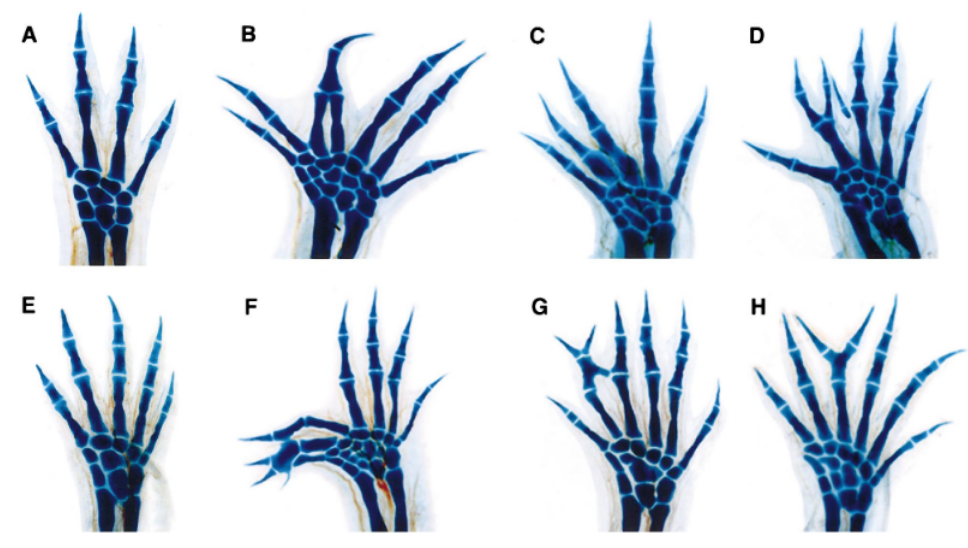
\includegraphics[width=0.8\textwidth, page=1] {figures/introduction/fig3.png}
    \caption[Radiographies de squelettes régénérés de membres antérieurs et postérieurs d'axolotls avec ou sans injection d'un virus Vaccinia exprimant le gène \acrshort{SHH}.]{
    \textbf{Radiographies de squelettes régénérés de membres antérieurs et postérieurs d'axolotls avec ou sans injection d'un virus Vaccinia exprimant le gène \acrshort{SHH}} \textbf{A et E} :  Régénération normale d'un membre antérieur et postérieur chez un axolotl sans injection. \textbf{B-D} :  Régénération d'un membre antérieur après injection, présentant des doigts et des carpiens supplémentaires. \textbf{F-H} : Régénération d'un membre postérieur après injection, présentant des doigts et des tarses supplémentaires. Tirées de \citep{roy_vaccinia_2000}.\\
    }
    \label{fig:Fig3}
\end{figure} 

Ces conséquences soulignent l’importance de la régulation spatio-temporelle de l’expression des gènes dans l'établissement des phénotypes des organismes.

    \chapter{La régulation de l’expression}
{\hypersetup{linkcolor=GREYDARK}\minitoc}
\label{chap:regulation-de-expression}

Chez les organismes multicellulaires, l’activité des gènes est contrôlée à plusieurs niveaux et par de nombreux systèmes de régulation \citep{maston_transcriptional_2006}. Cette régulation peut se faire avant la transcription, par exemple par des modifications épigénétiques qui contrôlent l’accessibilité de la séquence, ou après la transcription, par exemple par la régulation de la stabilité des \acrshort{ARN} messagers. Une partie essentielle du contrôle de l’expression des gènes s’effectue cependant au niveau transcriptionnel, sur lequel je me suis concentré pendant ma thèse.

\section{Organisation de l’ADN dans le noyau}
\label{sec:organisation-ADN}

Dans les cellules eucaryotes, l’information génétique est organisée en une structure complexe, la chromatine, constituée d'\acrshort{ADN} et de nombreuses protéines \citep{kornberg_chromatin_1992}. Il s’agit d’une structure qui assure un degré de compaction dynamique de l’ADN et entraîne une accessibilité variable de la séquence aux machineries protéiques régulant les fonctions essentielles des génomes comme la réplication, la recombinaison, la réparation ou la transcription \citep{felsenfeld_controlling_2003}. La compaction de la chromatine peut être observée à de nombreuses échelles (Figure \ref{fig:Fig4}), mais je m’intéresserai ici plus particulièrement à son unité la plus fondamentale : le nucléosome. Il s’agit du premier niveau de compaction de la chromatine, qui contient 146 ou 147 nucléotides enroulés autour d’un complexe de quatre histones différentes, chaque histone étant présente en double exemplaire pour former un octamère d’histones. Les histones forment une famille de protéines spécialisées dans la formation des nucléosomes et sont parmi les protéines les plus conservées chez les eucaryotes \citep{sandman_diversity_1998}. Leurs extrémités sont la cible de modifications post-traductionnelles (méthylation, acétylation, phosphorylation...) qui peuvent affecter la structure de l’histone. De telles modifications peuvent influencer l’accessibilité de la séquence d’ADN y étant enroulée, ainsi que les interactions protéines-protéines de la chromatine. L’organisation de l’ADN dans le noyau par sa compaction et les modifications de la chromatine forment ainsi un des premiers mécanismes impliqués dans la régulation de la transcription des gènes.

\begin{figure}[h]
 \centering
 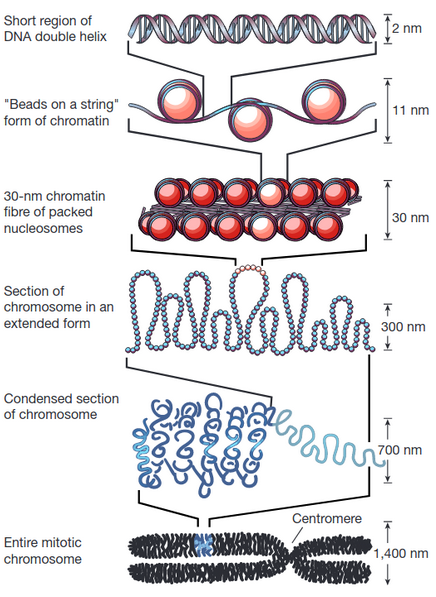
\includegraphics[width=0.5\textwidth, page=1] {figures/introduction/fig4.png}
 \caption[Organisation de l'\acrshort{ADN} au sein de la structure chromatinienne.]{
 \textbf{Organisation de l'\acrshort{ADN} au sein de la structure chromatinienne.}
 De haut en bas. Une région en double hélice d'\acrshort{ADN}. Le premier niveau de compaction est le nucléosome, dans lequel l'\acrshort{ADN} est enroulé autour de l'extérieur d'un octamère d'histone. Les nucléosomes sont reliés les uns aux autres par de courtes portions d'\acrshort{ADN} de liaison. Au niveau d'organisation suivant, la chaîne de nucléosomes est repliée et condensée en une fibre d'environ 30 nm de diamètre. Ces fibres sont ensuite repliées en structures d'ordre supérieur. Aux niveaux de structure au-delà du nucléosome, les détails du repliement sont encore incertains. Tirée de \citet{felsenfeld_controlling_2003}. \\
 }
 \label{fig:Fig4}
\end{figure} 

\section{La régulation transcriptionnelle}
\label{sec:reg-transcription}

La régulation transcriptionnelle des gènes est présente dans tous les systèmes cellulaires \citep{ptashne_regulation_2005}. Elle se fait grâce à des éléments \gls{trans}-régulateurs, c'est-à-dire des séquences d’ADN dont les produits (protéines ou \acrshort{ARN}s) circulent dans le noyau des cellules et interagissent avec différents loci pour réguler l’expression de leurs gènes cibles. Les produits des éléments \gls{trans}-régulateurs, aussi appelés \textit{trans}-facteurs, peuvent se fixer sur des séquences \gls{cis}-régulatrices, qui quant à elles vont avoir une action locale sur le même chromosome que leurs gènes cibles. La transcription des gènes chez les eucaryotes est ainsi un processus complexe qui nécessite l’orchestration d’interactions entre de multiples protéines, des \acrshort{ARN}s et des séquences d’ADN \citep{maston_transcriptional_2006,ong_enhancer_2011}.

\subsection{Les facteurs \textit{trans}-régulateurs}
\label{subsec:elem-trans}

\subsubsection{Les facteurs de transcription}
\label{subsubsec:facteur-trans}

Les facteurs de transcription (\acrshort{FT}s) sont des protéines qui se fixent généralement à l’ADN grâce à leur affinité avec de courtes séquences spécifiques de 6 à 16 nucléotides appelées des motifs de fixation, pouvant être plus ou moins nombreux et/ou stricts. Ces protéines contrôlent l’initiation, la progression ou l’arrêt de la transcription d’un ou plusieurs gènes. Chaque \acrshort{FT}, selon son ou ses motifs de fixation, peut se fixer à de nombreuses séquences dans le génome et ainsi participer à la régulation de plusieurs gènes à la fois. Les régions où se fixent les \acrshort{FT}s sont généralement enrichies en plusieurs sites de fixation de \acrshort{FT}s différents et sont appelées des séquences \gls{cis}-régulatrices.\\

Les \acrshort{FT}s forment généralement des complexes avec d’autres \acrshort{ARN}s ou protéines (ARN polymérase, enzymes, \acrshort{FT}s,…). Leurs modes d’actions sont variés, ils peuvent par exemple participer aux recrutements de différentes molécules impactant la régulation des gènes cibles ou participer à l’élaboration de boucles de chromatine. Le rôle fonctionnel d’un \acrshort{FT} est très dépendant de la diversité et de la concentration de plusieurs autres co-facteurs dans les cellules. Un même \acrshort{FT}, en présence de différents co-facteurs, pourra agir différemment ou sur l’expression de différents gènes ce qui le rend potentiellement très \gls{pleiotrope}. C’est alors la combinaison de plusieurs facteurs de transcription fixés sur une même séquence qui a un effet particulier sur les gènes cibles dans chaque type cellulaire. \\

On estime actuellement qu’il existe plus de 1500 gènes codants pour des facteurs de transcription dans le génome humain \citep{wingender_tfclass_2018}. Selon leurs motifs de fixation, les \acrshort{FT}s peuvent réguler un nombre très variable de gènes. De plus, la transcription de ceux-ci étant elle-même régulée, le patron d’expression des \acrshort{FT}s peut être variable, ceux-ci peuvent être spécifiques à un type cellulaire jusqu'à largement ubiquitaire.

\subsubsection{Les ARNs non-codants}
\label{subsubsec:ARN-noncodant}

La régulation de l’expression des gènes par des éléments agissant en \gls{trans} se fait également par le moyen d’\acrshort{ARN}s non-codants. En effet, la transcription d’un très grand nombre de gènes dans les génomes eucaryotes résulte en \acrshort{ARN}s ne codant pas pour des protéines. Certains de ces \acrshort{ARN}s participent à la régulation de l’expression des gènes. Les micro-\acrshort{ARN}s, composés d’une vingtaine de bases, sont les \acrshort{ARN}s non-codants dont les modes d’action sont peut-être les mieux compris \citep{bartel_micrornas_2004}. Ceux-ci se fixent de manière complémentaire aux \acrshort{ARN}s messagers produits par leurs gènes cibles. Après fixation, les microARN peuvent initier un clivage de l’\acrshort{ARNm} en plusieurs morceaux, ce qui déstabilise sa structure et entraîne une dégradation rapide. Cette fixation peut également perturber ou empêcher la traduction des \acrshort{ARNm} en protéine, inhibant alors l’expression des gènes cibles \citep{bartel_micrornas_2004}. De la même façon que les \acrshort{FT}s, les micro-\acrshort{ARN}s peuvent influencer l’expression d’un nombre très variable de gènes, pour certains jusqu’à plusieurs centaines de gènes. Bien que seulement un faible nombre soit caractérisé et validé expérimentalement, il existerait plus de 2000 micro-\acrshort{ARN}s dans le génome humain \citep{alles_estimate_2019}.\\

Les longs \acrshort{ARN}s non-codants, qui peuvent être composés de plusieurs milliers de bases, sont également une classe importante de régulateurs de l’expression des gènes. Ils peuvent agir à la manière des facteurs de transcription, en participant à la formation de complexes moléculaires ou en recrutant d’autres co-facteurs au niveau de l'initiation et l’élongation de la transcription. Par exemple il a été proposé que l’ARN non codant HOTAIR, participe à la modification de la chromatine dans la région des gènes \textit{HoxD} et interagit avec un complexe Polycomb répressif pour inhiber l’expression des gènes \citep{rinn_functional_2007}.

\subsection{Les séquences \textit{cis}-régulatrices}
\label{subsec:elem-cis}

Les séquences \gls{cis}-régulatrices sont des régions non-codantes de l’ADN qui régulent la transcription d’un ou plusieurs gènes selon leur accessibilité, leurs marques épigénétiques et les facteurs de transcription qui y sont fixés. Elles sont essentielles pour contrôler où, quand et comment un gène cible est activement transcrit. On distingue les promoteurs des gènes, situés immédiatement en amont du gène qu’ils régulent, et les éléments \gls{cis}-régulateurs plus distaux (Figure \ref{fig:Fig5}).

\begin{figure}[h]
 \centering
 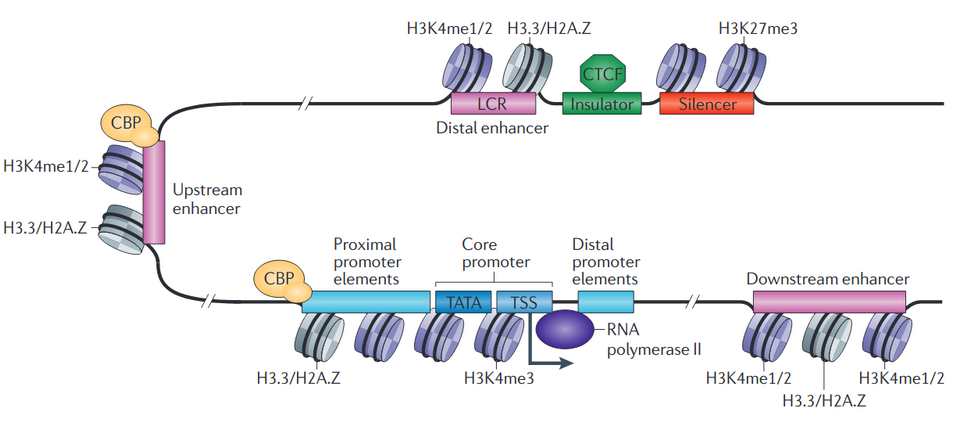
\includegraphics[width=0.8\textwidth, page=1] {figures/introduction/fig5.png}
 \caption[Diversité des éléments \gls{cis}-régulateurs.]{
 \textbf{Diversité des éléments \gls{cis}-régulateurs.}
 La séquence promotrice d'un gène (rectangles bleus) est généralement découpée en trois régions de tailles variables: proximale, centrale et distale, et contiennent notamment des sites de fixation de facteurs de transcription. La région centrale contient la séquence TATA qui permet la fixation de l'\acrshort{ARN} polymérase II et le site d'initiation de la transcription du gène (\acrshort{TSS}). La transcription d'un gène peut également être régulée par de nombreuses séquences en amont ou en aval, dont des \glspl{amplificateur} (rose), des \glspl{inhibiteur} (rouge) ou des isolateurs (vert). La présence de modifications sur les histones des nucléosomes (palets bleu et gris) et la présence de certaines protéines (jaune) au niveau de la chromatine permettent de détecter les séquences \gls{cis}-regulatrices et de mesurer leur activité. 
 
 Abréviations : CBP = Cyclic AMP-responsive element-Binding Protein. H3K4me1/2 = histone H3 mono- or dimethylation at lysine 4; H3K4me3 = histone H3 trimethylation at lysine 4; H3K27me3 = histone H3 trimethylation at lysine 27; H3.3/H2A.Z = histone variants H3.3 and H2A. Tirée de \citet{ong_enhancer_2011}.
 }
 \label{fig:Fig5}
\end{figure} 

\subsubsection{Les promoteurs des gènes}
\label{subsubsec:prom}

Les séquences principales de la régulation transcriptionnelle sont les promoteurs des gènes. La plupart des promoteurs contiennent une séquence spécifique d’une trentaine de nucléotides connue sous le nom de boîte TATA permettant la liaison de l’ARN polymérase II, essentielle à la transcription du gène. La présence au niveau du promoteur de certains facteurs de transcription dits “basaux” comme IIB est également nécessaire pour placer et stabiliser la polymérase avant d’initier la transcription \citep{kostrewa_rna_2009}. Ces facteurs se fixent spécifiquement sur des régions du promoteur d’environ 1 kb qui peuvent être caractérisées par leur enrichissement en dinucléotides \acrshort{CpG}, appelés îlots \acrshort{CpG} \citep{down_computational_2002, deaton_cpg_2011}. La méthylation des cytosines sur ces dinucléotides peut jouer un rôle important dans la compaction de l’ADN et alors influencer l’expression des gènes y étant associés \citep{moore_dna_2013}. De plus, l’ARN polymérase II ne se fixe pas sur tous les promoteurs accessibles du génome en même temps. Son recrutement et sa stabilisation sur les promoteurs dépend de l’accessibilité de la séquence mais également d’autres séquences \textit{cis}-régulatrices plus éloignées.

\subsubsection{Les éléments \textit{cis}-régulateurs distaux}
\label{subsubsec:cis-reg}

Les éléments \gls{cis}-régulateurs distaux sont des séquences capables de fixer des combinaisons de facteurs de transcription et pouvant interagir avec les promoteurs de gènes de manière spécifique via des complexes de protéines et/ou des repliements de la chromatine. Selon les facteurs de transcription qui s’y fixent, ces éléments peuvent être de trois types : \glspl{amplificateur} de l’expression des gènes (“enhancer” en anglais), \glspl{inhibiteur} de l’expression réduisant l’activité des gènes, et isolateurs qui permettent d’isoler certaines régions du génome pour limiter l’interaction des gènes avec d’autres séquences (Figure \ref{fig:Fig5}) \citep{maston_transcriptional_2006}. Dans ce manuscrit, je me concentrerai principalement sur les éléments \gls{cis}-régulateurs identifiés comme \glspl{amplificateur}, qui représentent la catégorie la mieux connue à ce jour. Cependant, il est nécessaire de garder à l’esprit que les éléments \gls{cis}-régulateurs sont très modulables. Une même séquence agissant comme \gls{amplificateur} dans un tissu pourra agir comme \gls{inhibiteur} dans un autre avec une combinaison différentes de facteurs de transcription y étant fixés \citep{gisselbrecht_transcriptional_2020, huang_enhancer-silencer_2022}. De plus les relations fonctionnelles entre un gène et un élément \gls{cis}-régulateur peuvent fortement dépendre des \glspl{condition} biologiques de la cellule. \\

La localisation génomique des éléments \gls{cis}-régulateurs est très hétérogène. Ils peuvent être situés à proximité de la séquence des promoteurs, en amont ou en aval \citep{maniatis_regulation_1987}. Mais ils peuvent aussi se situer à plus grande distance jusqu’à plusieurs mégabases des gènes qu’ils régulent \citep{visel_chip-seq_2009}. Ils peuvent également se situer dans les introns des gènes, comme c’est le cas d’un \gls{amplificateur} de \acrshort{SHH} nommé \acrshort{ZRS} situé dans un intron du gène \textit{LMBR1} à plus de 800kb de \acrshort{SHH} (Figure \ref{fig:Fig6}.A) \citep{lettice_long-range_2003}. Les gènes les plus proches d’un élément \gls{cis}-régulateur ne sont donc pas nécessairement les cibles de celui-ci. Il existe différents mécanismes pour rapprocher spatialement un \gls{amplificateur} de son promoteur cible. Ce rapprochement peut se faire à travers la mise en place de complexes protéiques ou par la formation de boucles de la chromatine, ces deux mécanismes n’étant pas exclusifs (Figure \ref{fig:Fig6}.B).\\

\begin{figure}[h]
 \centering
 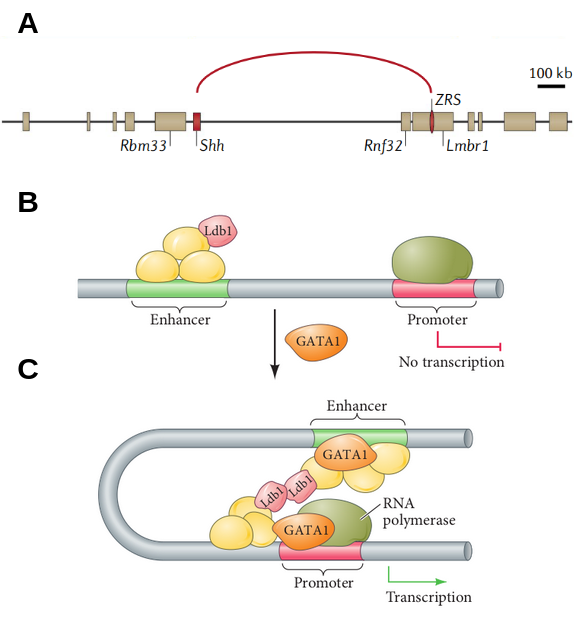
\includegraphics[width=0.7\textwidth, page=1] {figures/introduction/fig6.png}
 \caption[Interaction à grande distance entre promoteur et \gls{amplificateur}.]{
 \textbf{Interaction à grande distance entre promoteur et \gls{amplificateur}.}
 \textbf{A.} Localisation génomique du gène \acrshort{SHH} et de son \gls{amplificateur} \acrshort{ZRS} situé à plus de 800kb dans un intron du gène \textit{LMBR1}.
 \textbf{B et C} Schéma de la formation d'une boucle de chromatine entre un \gls{amplificateur} (vert) fixant des facteurs de transcription et le promoteur d'un gène (rouge) fixant l'\acrshort{ARN} polymérase II. Dans cet exemple c'est le facteur de transcription GATA1 qui assure la liaison entre les deux séquences pour permettre la transcription du gène.\\
 }
 \label{fig:Fig6}
\end{figure}

Les \glspl{amplificateur} sont souvent essentiels au recrutement de la machinerie d’initiation de la transcription mais aussi au déplacement de l’ARN polymérase du promoteur vers le corps du gène, permettant l’élongation de la transcription \citep{zippo_histone_2009}. Ils contrôlent l’efficacité et le taux de transcription d’un gène cible à partir de son promoteur. La transcription chez les eucaryotes fonctionne de manière discontinue, avec des cycles d’activité entrecoupés par des périodes d’arrêts \citep{chubb_transcriptional_2006, raj_stochastic_2006}. L’activité d’un \gls{amplificateur} et/ou l’action conjointe de plusieurs éléments peuvent augmenter la fréquence des ces cycles d’activité. De plus, la transcription des gènes eucaryotes nécessite la décompaction de la chromatine afin d’augmenter l’accessibilité de l’ADN à d’autres protéines comme la polymérase et les facteurs de transcription. Cette tâche peut également être initiée par les \glspl{amplificateur} en fixant des facteurs de transcription. Ces derniers peuvent recruter à leur tour des enzymes de modification des histones ou encore des complexes de remodelage de la chromatine pour altérer sa structure. Il a aussi été montré que les \glspl{amplificateur} peuvent être transcrits en des \acrshort{ARN}s non-codants ou \acrshort{eRNA} (pour “enhancer-RNA” en anglais) \citep{santa_large_2010}. La concentration des \acrshort{eRNA} est corrélée positivement avec l’activité de l’\gls{amplificateur}, mais aussi avec la production d’\acrshort{ARNm} des gènes cibles. Ceci suggère que les \acrshort{eRNA} sont produits lorsqu’ils sont en contact avec le promoteur d’un gène activement transcrit \citep{cheng_genome-wide_2015}. Cette production de transcrits \acrshort{eRNA} pourrait être un simple effet collatéral de la présence de l’ARN polymérase II sur la séquence de l’\gls{amplificateur}. L’\gls{amplificateur} serait alors transcrit mais le produit de cette transcription n’aurait pas de fonction en lui-même \citep{struhl_transcriptional_2007}. Plusieurs études suggèrent cependant que certains de ces \acrshort{eRNA} pourraient jouer des rôles importants dans la régulation de la transcription des gènes situés en \gls{cis}, c'est à dire sur le même chromosome, notamment par leur capacité à recruter des protéines de modification de la chromatine \citep{wang_reprogramming_2011, arnold_diversity_2020}. Une certaine classe de \acrshort{eRNA} a également montré une capacité d’induire et de stabiliser des contacts spécifiques entre promoteurs des gènes et éléments \gls{cis}-régulateurs sans l’intermédiaire de protéine de remodelage de la chromatine \citep{wang_reprogramming_2011}. Finalement, certains \acrshort{eRNA} plus stables et donc moins vite dégradés, pourraient agir comme régulateurs de gènes localisés sur un autre chromosome (en \gls{trans}) en se fixant de manière spécifique sur d’autres \glspl{amplificateur} \citep{cajigas_evf2_2018}. Les mécanismes de fonctionnement des \glspl{amplificateur} ne sont pas encore parfaitement connus mais sembleraient donc être très variés. Ceux-ci peuvent en effet agir comme attracteurs de facteurs de transcription, régulateurs de la machinerie de transcription, modificateurs de la chromatine, inducteurs de boucle d’ADN et régulateurs en \gls{trans}.

\subsection{Contribution des mécanismes en \textit{trans} et en \textit{cis}}
\label{subsec:contrib-cis-trans}

L’importance relative de la régulation en \textit{trans} et en \gls{cis} dans l’expression des gènes peut-être complexe à évaluer. Dans une expérience originale de transgénèse, Wilson et collaborateurs ont testé si les différences d’expression des gènes entre la souris et l’humain étaient dirigées par la séquence génétique ou par l’environnement nucléaire \citep{wilson_species-specific_2008}. Suite au transfert du chromosome 21 humain dans les cellules d’une souris transgénique, ils ont observé que la distribution des sites de fixation des facteurs de transcription sur ce chromosome dans les cellules de souris était similaire à la distribution observée dans les cellules humaines. De même, le patron d’expression des gènes localisés sur le chromosome 21 était similaire à celui observé chez l’humain, et non pas à celui des gènes homologues chez la souris. Cette observation est également valable pour le patron d’épissage des gènes codants pour des protéines \citep{barbosa-morais_evolutionary_2012}. Ainsi, la séquence génétique et donc les éléments \gls{cis}-régulateurs semblent être majoritairement responsables du patron d’expression et d’épissage de ces gènes et non pas les facteurs \gls{trans}. Les différences interspécifiques de l’environnement cellulaire et des éléments agissant en \gls{trans}, tels que les facteurs de transcription ou certains \acrshort{ARN} non-codants, joueraient des rôles secondaires. Ceci semble alors indiquer que, même si les sites de fixation en \gls{cis} ont pu évoluer entre les deux espèces, les facteurs agissant en \gls{trans} présentent une forte conservation évolutive. Ce résultat est attendu car les facteurs de transcription possèdent de nombreuses fonctions distinctes et sont sous une forte sélection purifiante \citep{wray_evolutionary_2007}. Des modifications de leurs séquences engendreraient des conséquences majoritairement délétères sur la valeur sélective de l’organisme. \\

Des changements d’expression de certains régulateurs agissant en \gls{trans} pourraient néanmoins participer aux différences du niveau d’expression des gènes. C’est par exemple le cas pour des microARNs dont la différence d’expression expliquerait une part importante de la divergence d’expression de leurs gènes cibles dans le cerveau des primates \citep{hu_microrna_2011}. L’émergence spécifique d’éléments agissant en \gls{trans} pourrait également permettre des changements de l’expression de gènes et potentiellement avoir un rôle important dans l'évolution phénotypique. Par exemple, le microARN miR-934 spécifique des primates et exprimé lors de la neurogénèse chez l’humain est associé à des changements majeurs du patron d’expression de plusieurs gènes impliqués dans la prolifération et la différentiation des neurones \citep{prodromidou_microrna-934_2020}.

\section{Identification et caractérisation des séquences \textit{cis}-régulatrices}
\label{sec:identif-cis}

Au cours de ma thèse, je me suis concentré sur les séquences \gls{cis}-régulatrices, qui sembleraient être les plus susceptibles de contribuer aux changements de l’expression des gènes. Un des premiers enjeux est alors de détecter ces séquences non-codantes dans les génomes. De nombreuses méthodes existent actuellement pour détecter, identifier et caractériser des séquences qui pourraient potentiellement être impliquées dans les changements d’expression des gènes (Figure \ref{fig:Fig7}). Elles permettent de prédire, plus ou moins précisément, des séquences \gls{cis}-régulatrices candidates. Elles ont dévoilé l’existence de plusieurs centaines de milliers d’\glspl{amplificateur} dans les génomes, dépassant largement le nombre de gènes protéiques. Ces découvertes démontrent l’importance de la régulation de la transcription en tant que premier niveau de contrôle du génome et donc des fonctions de l’organisme. Je vais ici détailler quelques-unes des grandes catégories d’approches utilisées pour identifier les séquences \gls{cis}-régulatrices et dont certaines ont fourni des données essentielles à mes travaux durant cette thèse. \\

\begin{figure}[h]
 \centering
 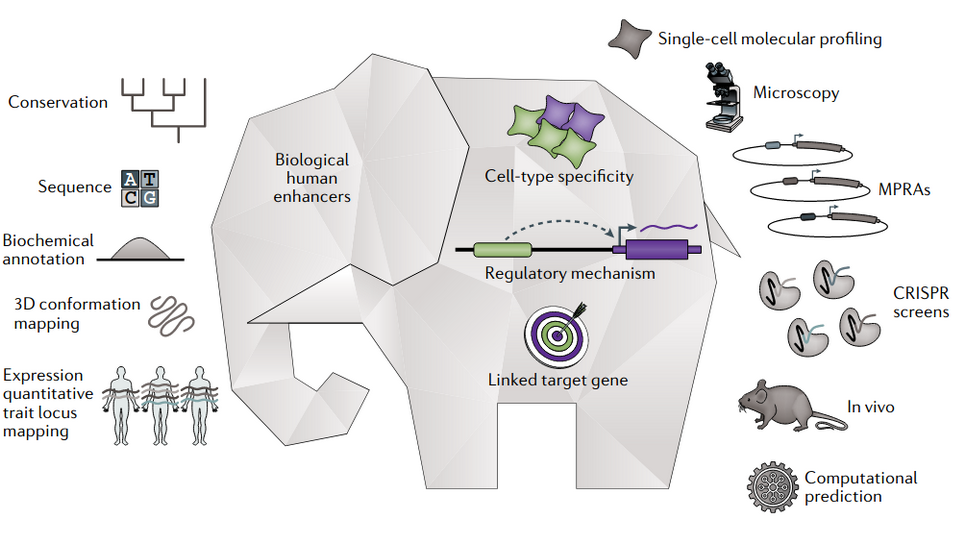
\includegraphics[width=0.9\textwidth, page=1] {figures/introduction/fig7.png}
 \caption[Diversité des méthodes de détection et de caractérisation de la fonction des éléments \gls{cis}-régulateurs.]{
 \textbf{Diversité des méthodes de détection et de caractérisation de la fonction des éléments \gls{cis}-régulateurs.}
 Dans une revue récente, Gasperini et collaborateurs font une analogie entre les différentes méthodes qui tentent de décrire les éléments \gls{cis}-régulateurs et un ancien compte indien où des aveugles tentent de décrire un éléphant en touchant chacun une partie différente. L'ensemble des méthodes, aussi hétérogènes et biaisées soit-elles peuvent être complémentaires et permettent d'obtenir différents aperçus d'une même réalité. Tirée de \citet{gasperini_towards_2020}.
 }
 \label{fig:Fig7}
\end{figure}

\newpage
\subsection{Approches computationnelles}
\label{subsec:approch-comput}

\subsubsection{Association génotype-phénotype}
\label{subsubsec:geno-pheno}

La prédiction d’éléments \gls{cis}-régulateurs peut d'abord s'effectuer par l’association de variations génotypiques à des variations phénotypes. En analysant les séquences génomiques de plusieurs individus conjointement avec une mesure d’un trait phénotypique on peut corréler la fréquence d’une variation génétique avec le trait d'intérêt. Par exemple, la variation d’un nucléotide ou SNP (Single Nucleotide Polymorphism) peut être corrélée à la variation d’un trait quantitatif, on parlera alors de QTL (Quantitative Trait Locus). Lorsque le trait quantitatif auquel on s’intéresse est le niveau d’expression d’un gène, on parlera d’eQTL (expression QTL). Ces méthodes ne cherchent pas spécifiquement des éléments \gls{cis}-régulateurs mais toute séquence ou mutation associée à un trait, les eQTLs peuvent ainsi se situer dans des gènes comme dans des régions non-géniques. Dans ce dernier cas, ils peuvent signaler la présence d'éléments régulateurs. Les mécanismes moléculaires entre un eQTL et les variations de l’expression d’un gène ne peuvent pas être déterminés par cette méthode, ceux-ci pouvant se faire à l’ensemble des niveaux de régulation. \\

C’est notamment par des études d’association entre génotypes et phénotypes qu’au début des années 90 a été découverte la région contenant un \gls{amplificateur} du gène \acrshort{SHH}. Cet \gls{amplificateur} est spécifique du bourgeonnement des membres, et est appelé \acrshort{ZRS} pour “Zone of polarizing activity Regulatory Sequence”. Les études qui ont permis de découvrir \acrshort{ZRS} cherchaient à comprendre les bases génétiques de certaines malformations congénitales. Elles se basent sur l’analyse du génotype d’individus ou de familles présentant des malformations au niveau des membres chez l’humain comme la triphalangie du pouce, la polydactylie (nombre surnuméraire de doigts) ou plus rarement l’acheiropodie (absence de main et de pied) \citep{hing_linkage_1995, zguricas_clinical_1999}. En comparant les variations de plusieurs marqueurs génétiques, ces études ont pu associer ces malformations à la région 7q36 sur le chromosome 7 humain sans pour autant connaître son rôle régulateur. Parallèlement, l’analyse de l’expression de plusieurs gènes dans des embryons de souris mutantes polydactyles a permis d’identifier une expression anormale du gène \acrshort{SHH} comme potentiellement responsable de ce phénotype \citep{sharpe_identification_1999}. \\

Cependant les méthodes d'associations entre génotype et phénotype permettent seulement de détecter une association statistique entre un ou plusieurs loci et un phénotype donné. Elles sont donc grandement dépendantes du nombre d'individus étudiés et des variations de leurs séquences. Aujourd’hui, avec l’avancée des techniques moléculaires, les associations génotype-phénotype sont appliquées à grande échelle, sur un grand nombre d'individus et sur des génomes complets, améliorant grandement leur pouvoir statistique et donc prédictif. C’est le cas des études dites GWAS (Genome Wide Association Study) qui ont permis d’identifier de nombreuses séquences d’ADN polymorphes entre les génomes humains et étant potentiellement responsables de divers changements moléculaires \citep{lappalainen_evolutionary_2010, bryois_cis_2014}.

\subsubsection{Conservation évolutive}
\label{subsubsec:conserv-evol}

Les études de génomique comparative permettent de détecter des séquences non-codantes conservées à plus ou moins large échelle évolutive. Cette forte conservation peut être le signal d’un rôle fonctionnel important associé à des mécanismes de régulation de l’expression des gènes. Chez les vertébrés par exemple, la comparaison de séquences d’espèces divergentes de plus de 300 millions d’années a révélé des séquences hautement conservées dans les régions non-codantes des gènes \citep{duret_strong_1993}. Il a ainsi été proposé que ces séquences pourraient agir comme régulatrices de l’expression des gènes. Une autre analyse se basant sur les alignements de séquence de plusieurs espèces de mammifères sur le génome humain a montré que de nombreuses séquences non codantes appelées Ultra-Conserved-Elements (UCE) sont mieux conservées que des exons codants et certaines peuvent être retrouvées avec une forte similarité de séquence chez les poissons \citep{bejerano_ultraconserved_2004}. \\

De la même manière, pour \acrshort{SHH} et son \glspl{amplificateur} \acrshort{ZRS}, il a été montré que la séquence et la localisation dans le 5ème intron de \textit{LMBR1} de \acrshort{ZRS} sont très conservées entre l’humain, la souris et le poulet, et cette comparaison évolutive a permis de définir plus précisément sa région fonctionnelle à environ 1,2 kb (Figure \ref{fig:Fig8}) \citep{lettice_long-range_2003, sagai_elimination_2005}. De plus, malgré les différences morphologiques importantes entre les membres et les nageoires, un élément \gls{cis}-régulateur homologue de \acrshort{ZRS} est présent chez les poissons. La similarité de séquence entre l’élément  identifié chez le poisson et son homologue chez la souris a permis d’estimer le cœur fonctionnel de l’\gls{amplificateur} à environ 200 pb.

\begin{figure}[h]
 \centering
 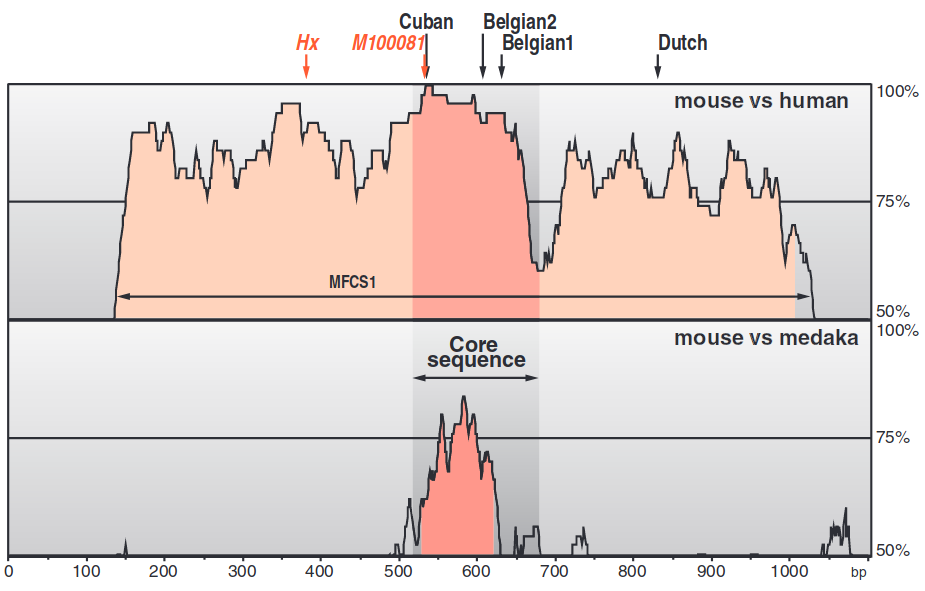
\includegraphics[width=0.8\textwidth, page=1] {figures/introduction/fig8.png}
 \caption[Conservation de la région contenant l'\gls{amplificateur} \acrshort{ZRS} (anciennement MFCS1) de la souris.]{
 \textbf{Conservation de la région contenant l'\gls{amplificateur} \acrshort{ZRS} (anciennement MFCS1) de la souris.}
 Pourcentage de similarité de séquence dans une partie de l'intron 5 de \textit{Lmbr1} entre la souris et l'humain en haut et entre la souris et le medaka (\textit{Oryzias latipes}, un poisson) en bas. Les flèches indiquent les sites où des mutations ponctuelles sont connues pour affecter l'expression de \acrshort{SHH} chez la souris (rouge) et chez l'humain (noir).
 MFCS1 = mammals-fishes-conserved-sequence 1.
 Tirée de \citet{sagai_elimination_2005}\\
 }
 \label{fig:Fig8}
\end{figure}

\subsection{Approches expérimentales}
\label{subsec:approch-expe}

\subsubsection{Ouverture de la chromatine et accessibilité de l’ADN}
\label{subsubsec:ouverture-chroma}

Les premières méthodes pour localiser les éléments fonctionnels actifs ont été développées à partir de l’identification de régions génomiques hypersensibles au clivage par la DNase I, une protéine dégradant l’ADN \citep{keene_dnase_1981, mcghee_200_1981}. Les régions où des modifications locales de la structure de la chromatine perturbent la compaction de l’ADN, comme les promoteurs de gènes activement transcrits, sont plus accessibles et donc plus faciles à digérer par la DNase I. Il a par la suite été montré que les sites hypersensibles à la DNase I (DHSs) sont généralement des régions de moins de 250 nucléotides et sont des marqueurs pour plusieurs catégories d'éléments \gls{cis}-régulateurs, y compris les promoteurs et les \glspl{amplificateur} \citep{felsenfeld_controlling_2003}. Le développement de méthodes de séquençage en haute résolution de ces sites, comme le DNase-seq, a ensuite permis de produire des cartes de l’état de la chromatine à l’échelle du génome entier. Grâce à cette technique par exemple, il a été démontré que dans les cellules T CD4+ humaines, plus de 80\% des DHSs sont localisés en dehors des promoteurs et des exons \citep{boyle_high-resolution_2008}. De plus les DHSs sont enrichis en variants associés à des changements phénotypiques ou à des maladies génétiques, ce qui conforte l’hypothèse d’un rôle majeur dans la régulation des gènes \citep{maurano_systematic_2012}. En combinant des mesures de DNase-seq sur un grand nombre d'échantillons, plusieurs études ont tenté de dresser un répertoire des DHSs du génome humain \citep{thurman_accessible_2012, meuleman_index_2020}. Par exemple, sur plus de 700 échantillons humains, une étude récente a permis de lister plus de 3,5 millions de DHSs et donc de potentiels éléments \gls{cis}-régulateurs \citep{meuleman_index_2020}. Des \textit{consortia} comme ENCODE ou RoadMap Epigenomics, dont l’objectif est d’identifier tous les éléments fonctionnels du génome de l’humain ou de la souris, collectent et mettent à disposition de nombreuses données telles que du DNase-seq avec des protocoles standardisés, ouvrant la voie à de nombreuses études \citep{davis_encyclopedia_2018, roadmap_epigenomics_consortium_integrative_2015}. Nous avons utilisé certaines de ces données comme prédiction des \glspl{amplificateur} au cours de ma thèse dans les travaux que je présenterai dans la Partie \ref{part:chap2} et \ref{part:chap3}. \\

En 2013, une technologie nommée ATAC-seq (“Assay for Transposase Accessible Chromatin with high throughput sequencing”) a été développée pour détecter l’ouverture de la chromatine et donc l’accessibilité de l’ADN de manière plus sensible et à moindre coût \citep{buenrostro_transposition_2013}. Elle se base sur l’activité d’une transposase hyperactive, une enzyme qui va insérer une séquence cible dans toutes les régions du génome où la chromatine est ouverte. Cette séquence intégrée va alors jouer le rôle d'adaptateur pour permettre d’amplifier les régions avoisinantes puis les séquencer à haut débit. Cette technique a facilité l’analyse et la découverte d’éléments \gls{cis}-régulateurs en simplifiant les expérimentations et en les rendant faisable sur un faible nombre de cellules \citep{daugherty_chromatin_2017}. Nous avons utilisé cette technique pour détecter les régions \gls{cis}-régulatrices candidates dans le tubercule génital du poulet et du canard que je détaillerai dans la Partie \ref{part:chap4}. 

\subsubsection{Modification d’histones}
\label{subsubsec:histone}

Les modifications post-traductionnelles des histones peuvent apporter des informations sur les fonctions des séquences. Le développement de méthodes expérimentales utilisant l’immuno-précipitation de la chromatine (ChIP) combinée initialement à des puces à ADN (ChIP-chip) ou plus récemment à du séquençage à haut débit (\acrshort{ChIP-seq}), a permis de déterminer les sites de l’ADN en liaison avec une protéine donnée \citep{ren_genome-wide_2000, barski_high-resolution_2007}. Cette protéine peut être une histone avec des modifications biochimiques précises, un facteur de transcription ou toute autre protéine capable de se fixer à l’ADN \citep{visel_chip-seq_2009}. Avec cette technique, la chromatine est précipitée en utilisant un anticorps spécifique de la protéine d’intérêt, les régions ainsi liées sont récupérées puis séquencées. Grâce à ces données, il a par exemple été montré que des niveaux élevés d'acétylation sur la 27ème lysine (K27) de l’histone H3 (notée H3K27ac) ou de méthylation sur la 4ème lysine du même histone (H3K4me) sont généralement détectés dans les régions promotrices des gènes actifs (Figure \ref{fig:Fig9})  \citep{bernstein_genomic_2005}. De même, des niveaux élevés de méthylation sur la 27ème lysine de l’histone H3 (H3K27me) sont corrélés à la répression des gènes \citep{lee_control_2006}. Ces modifications peuvent également être détectées dans les régions intergéniques. Les signaux d'acétylation de H3 (H3K27ac par exemple) et la mono-méthylation de H3K4 (H3K4me1) à l'extérieur des régions promotrices ont été corrélés avec la présence d’\glspl{amplificateur} \citep{heintzman_distinct_2007}. De nombreux \glspl{amplificateur}, actifs ou non, ont ainsi pu être prédits par ces marques épigénétiques \citep{creyghton_histone_2010}. Ces dernières ne sont pour autant pas toujours discriminantes de la fonction et de l’activité des séquences qui leur sont associées. Par exemple, des marques très similaires peuvent être présentes sur les promoteurs et les \glspl{amplificateur} actifs comme H3K27ac (Figure \ref{fig:Fig9}). Néanmoins, leur cartographie dans différents types cellulaires permettent de mieux identifier et caractériser les régions fonctionnelles. Les \textit{consortia} ENCODE et RoadMap Epigenomics cités plus haut mettent également à disposition de grands répertoires d’éléments non-codants potentiellement fonctionnels identifiés par ces modifications d’histones \citep{davis_encyclopedia_2018, roadmap_epigenomics_consortium_integrative_2015}.

\begin{figure}[h]
 \centering
 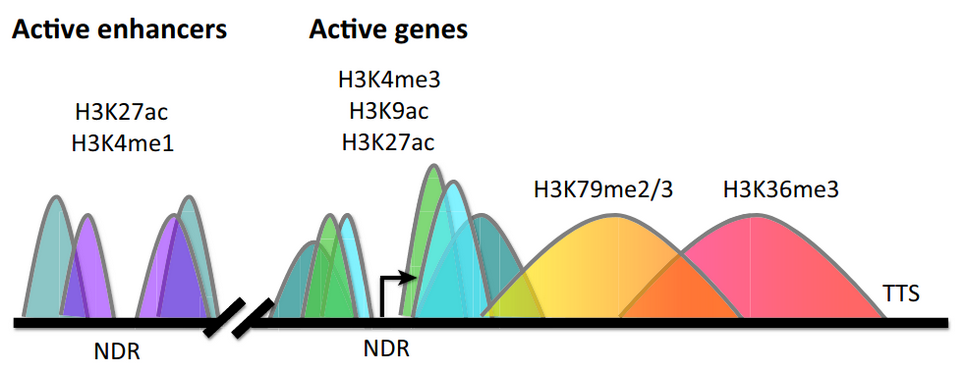
\includegraphics[width=0.8\textwidth, page=1] {figures/introduction/fig9.png}
 \caption[Localisation génomique des modifications d'histone H3 associées à la transcription active des gènes.]{
 \textbf{Localisation génomique des modifications d'histone H3 associées à la transcription active des gènes.}
 Schéma de l'occupation des modifications des histones H3 obtenus par les méthodes d'immunoprécipitation de la chromatine et de séquençage (\acrshort{ChIP-seq}). Les régions en couleur représentent un signal ChIP classique pour des \glspl{amplificateur} ou des gènes actifs.
 Gris, acétylation sur la lysine 27 de H3 (H3K27ac) ; violet, monométhylation sur la lysine 4 de H3 (H3K4me1) ; bleu clair, acétylation sur la lysine 9 de H3 (H3K9ac) ; vert, triméthylation sur la lysine 4 de H3 (H3K4me3) ; jaune, di- et triméthylation sur la lysine 79 de H3 (H3K79me2/3) ; rose/rouge, triméthylation sur la lysine 36 de H3 (H3K36me3). H3K4me3 et H3K9ac sont associés aux régions promotrices des gènes actifs, alors que H3K36me3 et H3K79me3 sont localisés dans les corps des gènes en cours de transcription. H3K27ac se localise à la fois au niveau des promoteurs des gènes actifs et des amplificateurs, et H3K4me1 est principalement enrichi au niveau des amplificateurs.
 Les gènes réprimés présentent des marques de méthylation différentes et pas d'acétylation d'histone (non montré). La flèche indique le site d'initiation de la transcription (\acrshort{TSS}). 
 Abréviations : NDR, région appauvrie en nucléosomes ; TTS, site de terminaison de la transcription. Tirée de \citet{bernstein_genomic_2005}.\\
 }
 \label{fig:Fig9}
\end{figure}

\subsubsection{Transcription des amplificateurs}
\label{subsubsec:eRNA}

Par défaut la présence de l'ARN polymérase II sur une séquence génère des transcrits courts dans les deux orientations (ou brins) de l'\acrshort{ADN} \citep{kim_widespread_2010, andersson_atlas_2014}. Au niveau des promoteurs classiques, des signaux supplémentaires permettent d'assurer l'élongation de la transcription des gènes dans une seule direction. L’ARN polymérase II peut cependant rester pendant un temps plus ou moins long sur les régions promotrices ainsi que sur les \gls{amplificateur} actifs avant l’élongation \citep{rougvie_rna_1988, mayer_pause_2017}. Durant ce laps de temps, ces derniers sont transcrits de manière bidirectionnelle, ce qui permet d'une part de les discriminer des autres transcrits \acrshort{ARN}s et d'autre part de quantifier leur activité. Cependant, même si leur stabilité peut être variable, ces transcrits sont généralement rapidement dégradés \citep{almada_promoter_2013}. Les méthodes classiques de \acrshort{RNA-seq} ne peuvent pas les détecter, mais ils peuvent être capturés et séquencés par des méthodes dédiées. \\

L’une d’elle nommée \acrshort{CAGE} ("Cap Analysis of Gene Expression"), s’appuie sur la capture et l’isolation de la coiffe présente sur l’extrémité 5’ des transcrits matures \citep{shiraki_cap_2003, andersson_atlas_2014}. Contrairement au séquençage \acrshort{RNA-seq} cette méthode cible et enrichit les premières bases des \acrshort{ARN}s, permettant de détecter les transcrits très courts et proches des sites d’initiation de la transcription (\acrshort{TSS}). Une autre technique, GRO-seq ("Global Run-On sequencing"), permet de mesurer de manière très sensible le taux de transcription des séquences engagées avec l’ARN polymérase II active \citep{core_nascent_2008}. Avec cette technique, les cellules sont mises en présence d’un nucléotide spécifique (le 5-bromouridine 5'-triphosphate) qui s'insère dans les \acrshort{ARN}s en cours de transcription. L'ajout de ce nucléotide aux transcrits permet ensuite de les isoler puis de les séquencer à haut débit. Le GRO-seq présente l’avantage de quantifier les fragments de transcrits naissants indépendamment de leur stabilité dans le noyau. Cette technique a notamment permis de détecter plusieurs \glspl{amplificateur} engagés avec un promoteur transcrit \citep{melgar_discovery_2011}. Les techniques de séquençage des éléments \gls{cis}-régulateurs transcrits ont permis d’identifier des \glspl{amplificateur} spécifiques de tissus et/ou de plusieurs stades de développement chez différentes espèces de mammifères, \textit{in vivo} ou \textit{in vitro}. Nous avons également utilisé des données publiques de GRO-seq et \acrshort{CAGE} dans le travail décrit dans la Partie \ref{part:chap3}).

\subsection{Validation fonctionnelle}
\label{subsec:validation}

Bien que de nombreuses méthodes permettent aujourd’hui d’identifier de potentiels éléments \gls{cis}-régulateurs à l’échelle de génomes entiers, il reste important de valider leur fonction exérimentalement et de déterminer précisement leurs impacts sur l’expression des gènes cibles. \\

Avec les contraintes évolutives apparentes des éléments non-codants ultra conservés (UCE) et leur relative proximité aux gènes, les premières études prédisaient déjà l’importance de ces séquences et leurs potentiels rôles dans la régulation de l’expression des gènes. Certains de ces UCE (n=167) ont été testés par des expériences de transgénèse chez des souris \citep{pennacchio_vivo_2006}. Pour tester la fonction de chaque UCE, celui-ci est injecté dans un embryon sous forme de plasmide et est associé avec un gène dit “rapporteur de l’expression” car la présence de ses protéines peut être visualisée par coloration ou fluorescence. Dans cette étude, c’est le gène \textit{LacZ} qui a été utilisé car il possède un promoteur minimal mais nécessite un \gls{amplificateur} actif pour produire des protéines dont l’activité enzymatique colore les cellules en bleu \citep{li_overview_2018}. Cette coloration permet de déterminer si un UCE donné joue effectivement un rôle d’\gls{amplificateur} et si oui dans quels tissus. Cette étude a ainsi montré que 45\% des séquences conservées testées sont des \glspl{amplificateur} de l’expression des gènes qui agissent dans un ou plusieurs tissus dans des embryons de souris au stade 11.5 (Figure \ref{fig:Fig10}) \citep{pennacchio_vivo_2006}. \\


\begin{figure}[h]
 \centering
 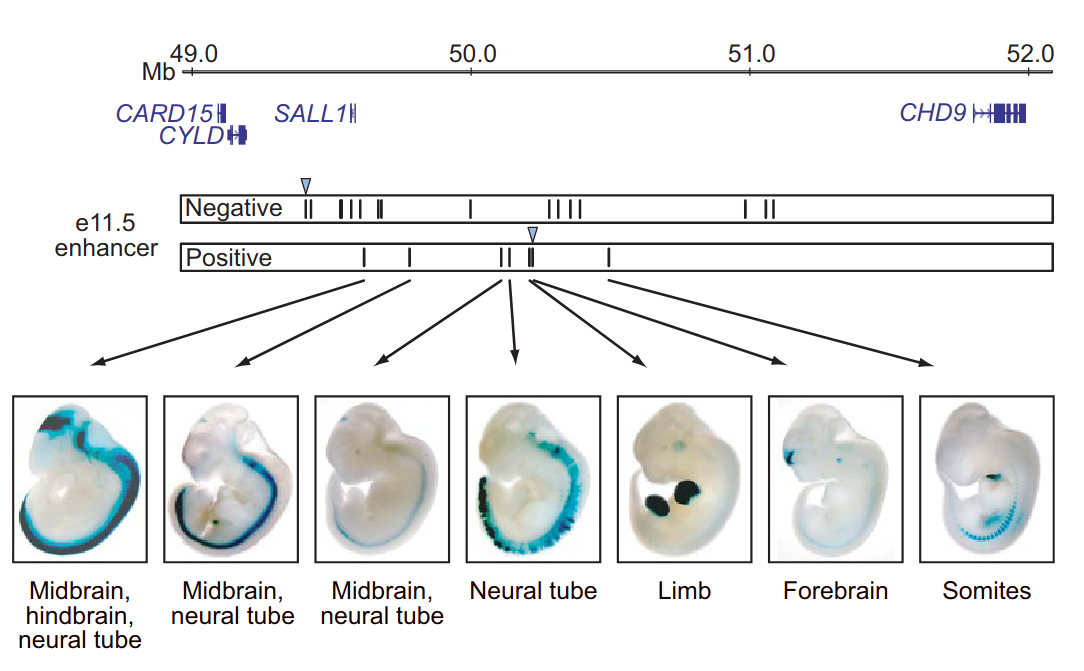
\includegraphics[width=0.8\textwidth, page=1] {figures/introduction/fig10.png}
 \caption[Validation de la fonction régulatrice de séquences non-codantes ultra-conservées.]{
 \textbf{Validation de la fonction régulatrice de séquences non-codantes ultra-conservées.} De haut en bas. Coordonnée génomique d'un fragment humain enrichi en éléments conservés chez le poisson-globe. Position des éléments humains testés dans une experience de transgénèse dans des embryons de souris. Les flèches bleues indiquent les éléments définis comme ultra-conservés. Les éléments sont classés comme "positif" ou "négatif" selon leur rôle d'activateurs de l'expression du gène \textit{LacZ} au 11,5ème jour du développement embryonnaire. Photographies des activités amplificatrices positives, la coloration bleue indique la localisation des protéines \textit{lacZ}. Tirée de \citet{pennacchio_vivo_2006}\\
 }
 \label{fig:Fig10}
\end{figure}

Afin de tester le rôle fonctionnel de l’\gls{amplificateur} \acrshort{ZRS} du gène \acrshort{SHH} et son implication dans les malformations des membres, Lettice et collaborateurs ont également effectué des expériences de transgénèse de la région contenant \acrshort{ZRS} dans des embryons de souris \citep{lettice_long-range_2003}. Cette étude a permis de confirmer le rôle activateur de l’expression de \acrshort{ZRS} dans le développement des membres. Ils ont également pu confirmer que de nombreuses mutations observées à des fréquences élevées dans les génomes d’individus présentant des polydactylies se localisent dans cette région. En effectuant des expériences de transgénèse de la séquence de \acrshort{ZRS} contenant certaines de ces mutations, une autre étude du même groupe a pu identifier un gain d’activité anormale dans plusieurs régions des membres (Figure \ref{fig:Fig11}) \citep{lettice_point_2008}. Cette nouvelle activité de \acrshort{ZRS} dans ces cellules active l’expression de \acrshort{SHH} et entraîne plusieurs malformations des membres. Par ailleurs, il a été montré que la délétion complète de l’\gls{amplificateur} \acrshort{ZRS} chez des souris entraîne des phénotypes similaires à l’inactivation complète du gène \acrshort{SHH} dans les membres, avec d’importantes malformations et des membres tronqués (Figure \ref{fig:Fig11}) \citep{sagai_elimination_2005}. 

\begin{figure}[h]
 \centering
 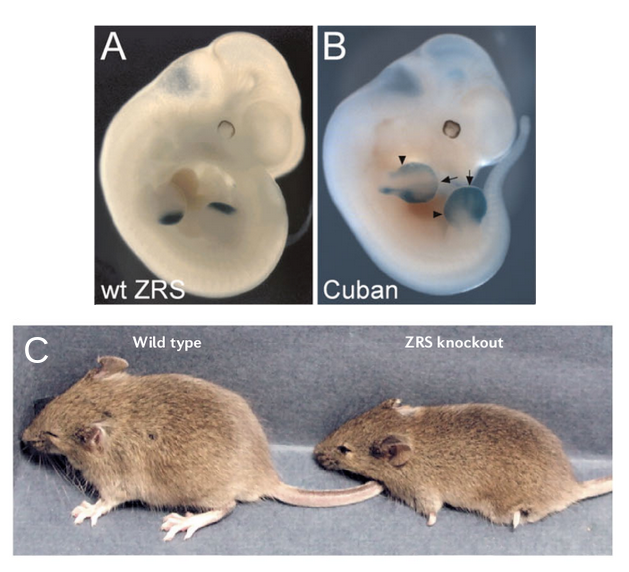
\includegraphics[width=0.6\textwidth, page=1] {figures/introduction/fig11.png}
 \caption[Validation de l'activité de l'\gls{amplificateur} \acrshort{ZRS}.]{
 \textbf{Validation de l'activité de l'\gls{amplificateur} \acrshort{ZRS}.}
 \textbf{A.} Photographie d'une expérience de transgénèse de la séquence normale de \acrshort{ZRS} de la souris dans un embryon de 11,5 jours, l'expression du gène rapporteur \textit{LacZ} (en bleu) a lieu dans la région postérieur des membres. 
 \textbf{B.} Transgenèse de la séquence de \acrshort{ZRS} comportant une mutation identifiée chez des patients atteints de polydactylie (identifiée sur une famille cubaine). Les flèches noires indiquent les régions des membres où une activité anormale est détectée. 
 \textbf{C.} Photographie d'une souris adulte normale et d'une souris aux membres tronqués où la séquence de \acrshort{ZRS} a été retirée du génome.
 Tirées de \citet{lettice_long-range_2003} et de \citep{sagai_elimination_2005}.\\
 }
 \label{fig:Fig11}
\end{figure}

L’importance fonctionnelle de nombreuses séquences \gls{cis}-régulatrices sur la morphologie, la physiologie et le comportement a été démontrée expérimentalement et chez plusieurs espèces \citep{wray_evolutionary_2007}. Cependant, la validation fonctionnelle des éléments \gls{cis}-régulateurs reste complexe et coûteuse. De plus, dans la grande majorité des cas, les relations entre éléments \gls{cis}-régulateurs et gènes sont très spécifiques d’un type cellulaire ou d’un contexte temporel ou environnemental, ce qui rend leur analyse délicate. Ainsi, l’accumulation de prédictions par différentes méthodes ou analyses est nécessaire afin de renforcer la confiance attribuée à chaque élément avant la validation de candidats d’intérêt. La base de données VISTA par exemple propose de recenser les éléments \gls{cis}-régulateurs validés expérimentalement \citep{visel_vista_2007}. Elle permet de confirmer des éléments non-codants prédits par l’accumulation de marques épigénétiques ou par une extrême conservation dans plusieurs espèces de vertébrés. Des expériences d’insertion des séquences prédites avec un marqueur de l’activité dans des embryons de souris sont ensuite menées pour tester leur fonctionnalité. Aujourd’hui plus de 3200 séquences ont été testés \textit{in vivo} chez la souris et plus de 1600 se sont révélés être des \glspl{amplificateur} actifs. \\

D’autres techniques ont également été développées pour tester l'activité amplificatrice d'un grand nombre de séquences en parallèles dans des lignées cellulaires \textit{in vitro}, comme le STARR-seq (“Self-Transcribing Active Regulatory Region sequencing”) ou le MPRA (“Massively Parallel Reporter Assays”) \citep{arnold_quantitative_2014, inoue_decoding_2015}. Celles-ci se basent principalement sur l’insertion d’un gène rapporteur de l’expression combiné à une séquence code-barre unique au niveau de nombreux loci d’intérêt à tester. Les séquences ayant un rôle d’\glspl{amplificateur} de l’expression permettent ainsi au gène intégré d’être transcrit. Après séquençage, il est possible de discriminer les différents transcrits à l’aide des codes-barre et ainsi identifier et quantifier l’activité des éléments \gls{cis}-régulateurs candidats. \\

Finalement, la validation fonctionnelle d’un \gls{amplificateur} n’est pas nécessairement synonyme d’effet direct sur l’expression des gènes. De nombreux mécanismes de compensation peuvent intervenir pour réduire l’effet d’un \gls{amplificateur} ou celui-ci peut ne simplement pas être associé à un gène dans un contexte cellulaire donné.

\section{Les contacts promoteur-amplificateur}
\label{sec:contact}

Pour obtenir un tableau complet du paysage \gls{cis}-régulateur d'un génome, il ne suffit pas d'identifier les éléments \gls{cis}-régulateurs mais il est également nécessaire de définir quels sont leurs gènes cibles. Certains éléments \gls{cis}-régulateurs peuvent se trouver séparés par plus d'un million de nucléotides des gènes qu’ils contrôlent, comme nous l’avons vu pour \acrshort{SHH} et l’\gls{amplificateur} \acrshort{ZRS}. Environ la moitié des éléments \gls{cis}-régulateurs se situeraient à plus de 250 000 paires de base de leur gène cible chez l’humain \citep{montavon_regulatory_2011}. Des repliements particuliers de l’ADN pourraient alors aider à mettre les éléments \gls{cis}-régulateurs en contact avec les promoteurs des gènes cibles pour assurer leurs fonctions régulatrices. De telles boucles de la chromatine ont été observées et permettent de rapprocher physiquement les gènes et les éléments \gls{cis}-régulateurs distaux \citep{tolhuis_looping_2002}. Ces structures, dont les déterminants et les conséquences sont un vaste champ d'étude actuel en biologie moléculaire, pourraient alors être essentielles pour assurer la régulation de l’expression des gènes.

\subsection{Impact sur la transcription}
\label{subsec:impact-transcription}

Différentes équipes ont cherché à comprendre si le contact entre \gls{amplificateur} et promoteur est essentiel à l’initiation de la transcription \citep{carter_long-range_2002}. Elles ont rapporté que les contacts s'établissent en même temps que la transcription des gènes, sans pouvoir distinguer s’ils sont la cause ou la conséquence de l'activation des gènes. Plusieurs études ont alors été menées pour induire expérimentalement un contact physique entre un \gls{amplificateur} et un gène tout en mesurant l’expression de celui-ci. Dans une première expérience, Deng et collaborateurs ont utilisé deux protéines à doigts de zinc (ZFP pour “zinc-finger protein”) se fixant spécifiquement à la séquence promotrice du gène de la Beta-globuline (\textit{Hbb}) de la souris pour l’une et à sa région régulatrice (LCR) pour l’autre \citep{deng_controlling_2012}. Chacune des ZFP est fusionnée avec un co-facteur de transcription LDB1 impliqué dans la formation de boucle d’ADN à grande distance en s’associant deux à deux (Figure \ref{fig:Fig12}.A). Ce contact forcé a entraîné une forte augmentation de la production d’\acrshort{ARNm} de \textit{Hbb}, démontrant que le contact entre le gène et l’\gls{amplificateur} peut augmenter la transcription du gène. Plus précisément, en utilisant le même modèle de contact forcé, Bartman et collaborateurs ont montré que l’augmentation de la fréquence du contact entre le promoteur de \textit{Hbb} et LCR entraîne une augmentation de la fréquence des pics d’activité de transcription du gène mais pas de leur durée \citep{bartman_enhancer_2016}. De plus, en ajoutant une ZFP associée avec LDB1 sur le gène de l’Alpha-globuline voisin de \textit{Hbb}, ce dernier est moins fréquemment transcrit. Cette dernière observation semble indiquer qu’il existerait une compétition des gènes pour le contact avec les \glspl{amplificateur}.

\begin{figure}[H]
 \centering
 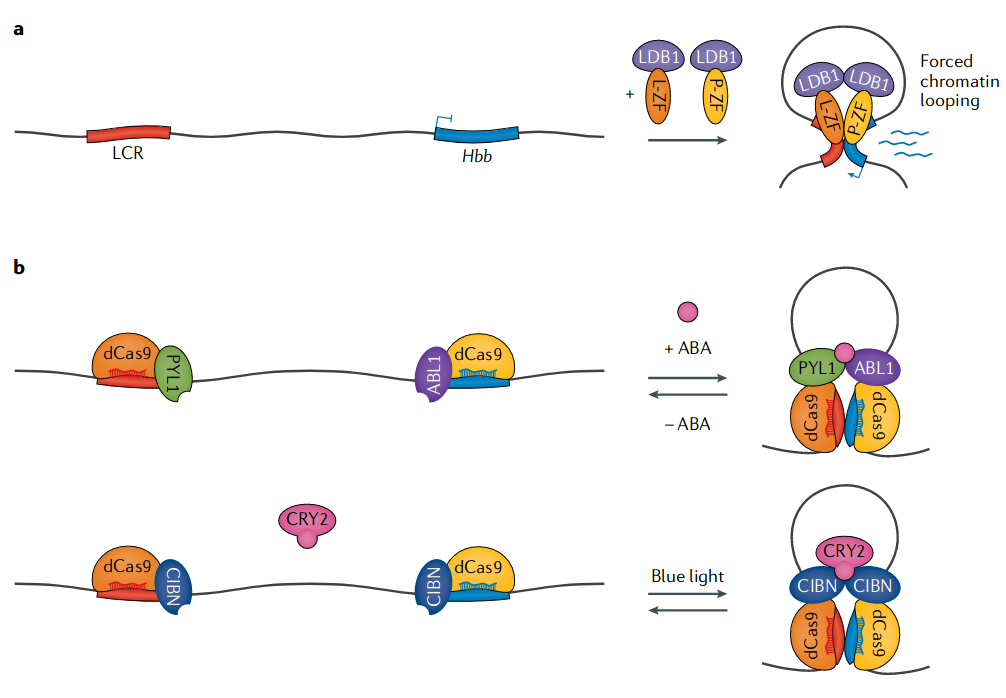
\includegraphics[width=0.8\textwidth, page=1] {figures/introduction/fig12.png}
 \caption[Techniques de contacts forcés entre promoteur et \gls{amplificateur}.]{
 \textbf{Techniques de contacts forcés entre promoteur et \gls{amplificateur}.}
 \textbf{A.} Contact forcé entre le promoteur de la Beta-globuline (\textit{Hbb}) de la souris et son \gls{amplificateur} LCR (locus control region). Des protéines à doigt de zinc fusionnées à une protéine LIM-domain binding 1 (LDB1) ciblent spécifiquement le promoteur de \textit{Hbb} (P-ZF) et la séquence de LCR (L-ZF). Ce contact forcé provoque l'augmentation de la transcription de Hbb \citep{deng_controlling_2012}.
 \textbf{\textbf{B.}} Contacts forcés à partir d'une variation de la machinerie CRISPR éditrice de génome. L'utilisation d'une nucléase-déficiente Cas9 (dCas9) permet de fusionner des protéines au niveau de séquences spécifiques. L'interaction réversible entre ces protéines permet ensuite de rapprocher les régions génomiques auxquelles elles sont fixées. Dans le premier cas, dCas9 est fusionné avec une protéine PYL1 (provenant de \textit{Streptococcus pyogenes}) sur un locus et une protéine ABL1 (provenant de \textit{Staphylococcus aureus}) sur un autre locus. Les deux protéines se dimérisent en présence d'acide abscissique (ABA) ce qui entraine le rapprochement des deux régions génomiques \citep{morgan_manipulation_2017}. Dans le second cas, les dCas9 sont fusionnées à des sous-unités de la protéine CIBN (provenant d'\textit{Arabidopsis thaliana}). En présence de protéines de cryptochrome 2 (CRY2) et de lumière bleu, les protéines CIBN forment un hétérodimère et rapprochent les régions sur lesquelles elles sont fixées \citep{kim_ladl_2019}. Tirée de \citet{schoenfelder_long-range_2019}.\\
 }
 \label{fig:Fig12}
\end{figure}

Pour aller plus loin dans la compréhension de ce mécanisme, des méthodes ont été développées pour forcer un contact entre un gène et son \gls{amplificateur} de manière contrôlable et réversible. Ceci a été possible grâce à l’utilisation d’un dérivé de la célèbre technique d’édition de séquence CRISPR-Cas9, qui fonctionne par l’action de l’enzyme de restriction Cas9 capable de se fixer à une séquence et de la découper en clivant les liaisons entre les nucléotides \citep{doudna_new_2014}. Dans cette approche, deux protéines Cas9 sont artificiellement modifiées pour se fixer à la séquence d’un promoteur pour l’une et d’un \gls{amplificateur} pour l’autre, mais sans les découper. Les Cas9 modifiées (dCas9) sont fusionnés avec des protéines qui, sous l’action d’un intermédiaire extérieur, vont pouvoir se rapprocher ou non (Figure \ref{fig:Fig12}.B). Dans la première étude décrivant cette méthode, l’intermédiaire extérieur est la présence ou non d’acide abscissique (ABA) \citep{morgan_manipulation_2017}. D’autres méthodes ont ensuite été développées, comme l’utilisation de lumière bleue agissant sur le cryptochrome 2 (CRY2) fusionné aux dCas9 et qui permet de rapprocher les loci \citep{kim_ladl_2019}. Dans les deux cas, ce contrôle sur le contact entre les deux séquences a permis de réguler de manière significative la transcription des gènes ciblés. Parallèlement, Bonev et collaborateurs ont découvert non seulement que les contacts entre \glspl{amplificateur} et promoteurs coïncident avec l'activation des gènes au cours de la différenciation des cellules souches de souris, mais aussi qu'ils sont interrompus lorsque les gènes sont réprimés \citep{bonev_multiscale_2017}. La microscopie confocale, couplée à des photographies à intervalle régulier, corrobore ce résultat en permettant de visualiser simultanément la transcription et la proximité entre promoteurs et \glspl{amplificateur} au cours du temps \citep{chen_dynamic_2018}.

\subsection{Formation et maintien des contacts}
\label{subsec:formation-contact}
\subsubsection{Facilitation des contacts : TADs et boucles CTCF}
\label{subsubsec:TAD-boucle}

D’après les contacts de chromatine observés, les génomes des métazoaires semblent être organisés en domaines de quelques mégabases à l’intérieur desquels les interactions entre loci sont facilitées \citep{sexton_role_2015, dixon_topological_2012, rao_3d_2014}. Ces domaines de contact connus sous le nom de \acrshort{TAD} (“Topologically Associating Domains”) permettent de partitionner le génome spatialement \citep{symmons_functional_2014}. Les contacts entre les éléments \gls{cis}-régulateurs et les promoteurs des gènes seraient favorisés à l’intérieur d’un même \acrshort{TAD} alors qu’ils seraient limités entre les \acrshort{TAD}s. Cela permettrait notamment de limiter l’influence d’éléments \gls{cis}-régulateurs non inclus dans un domaine et d’empêcher une activation aberrante des gènes. Ce rôle à la fois facilitateur et isolateur de contact pourrait avoir une importance majeure dans le contrôle de l’expression des gènes. \\

Les frontières de ces domaines sont enrichies en sites de fixation du facteur de transcription CTCF \citep{vietrirudan_comparative_2015}. CTCF est une protéine à doigts de zinc qui se fixe de manière directionnelle à l’ADN grâce à la reconnaissance d’un motif spécifique. Elle a été originellement identifiée comme \gls{inhibiteur} de l’expression de certains gènes \citep{filippova_exceptionally_1996} puis comme \gls{inhibiteur} de l’activité des \glspl{amplificateur} et aujourd’hui comme isolateur de régions d'\acrshort{ADN} \citep{bell_protein_1999}. En agissant conjointement avec la cohésine (un complexe protéique ayant une structure en anneau et de nombreux rôles dans la structuration de la chromatine), les sites de fixation de CTCF permettraient la formation de boucles d’ADN par un principe d’extrusion (Figure \ref{fig:Fig13}) \citep{sanborn_chromatin_2015}. Selon le modèle décrit par Sanborn et collaborateurs, le complexe de cohésine peut se fixer à l’ADN et initier la formation d’une petite boucle. Il est composé de deux sous-unités qui parcourent chacune l’ADN dans des directions opposées, élargissant la boucle de plus en plus. Chaque sous-unité du complexe d’extrusion est composée de protéine CTCF ce qui lui permet de s’arrêter lorsqu’elle rencontre son motif spécifique. Ce dernier n’est pas palindromique et est reconnu seulement dans une direction, de sorte qu’une boucle d’ADN ainsi formée sera composée de CTCF convergents à chacune de ces extrémités. La boucle qui résulte de cette extrusion engendre un domaine dans lequel les régions génomiques peuvent se rencontrer physiquement plus fréquemment. Une protéine nommée WAPL peut ensuite interagir avec la cohésine pour la détacher de l’ADN, ce qui libère le complexe formé et réduit la boucle d’ADN à son état d’origine. Les domaines formés par ce principe d’extrusion pourraient correspondre aux \acrshort{TAD}s observés dans les expériences de contacts de chromatine. \\

\begin{figure}[H]
 \centering
 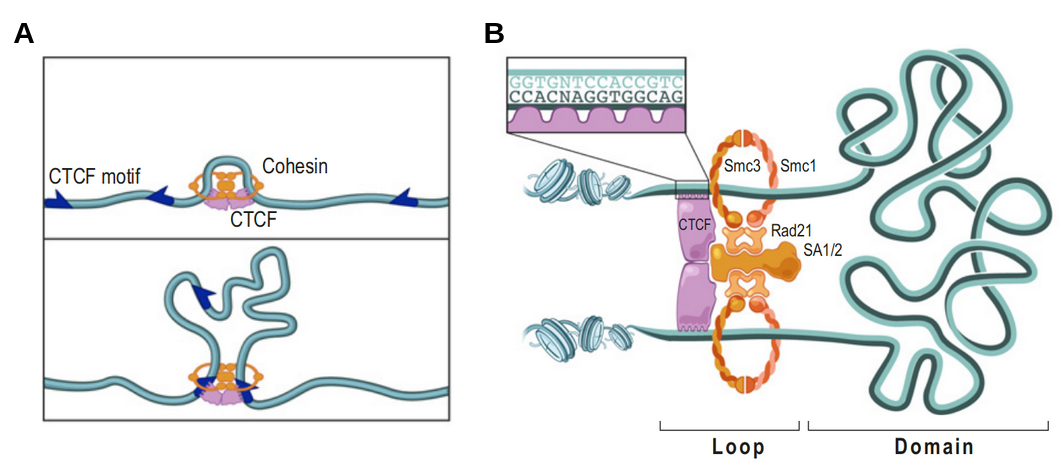
\includegraphics[width=0.8\textwidth, page=1] {figures/introduction/fig13.png}
 \caption[Formation d'une boucle d'\acrshort{ADN} par un principe d'extrusion.]{
 \textbf{Formation d'une boucle d'\acrshort{ADN} par un principe d'extrusion.}
 \textbf{A.} Un complexe protéique composé de deux anneaux de cohésine et de protéine CTCF se place sur l'ADN et initie une boucle. Ce complexe parcourt la séquence et agrandit la boucle jusqu'à la reconnaissance des motifs de CTCF. \textbf{B.} Vue complète de la formation d'un domaine plus large par principe d'extrusion. Tirée de \citet{sanborn_chromatin_2015}.
 \textbf{C.} Schéma de la formation de boucles d'ADN par un principe d'extrusion. \`A mesure que les complexes CTCF parcourent la séquence à divers endroits simultanément, les boucles s'agrandissent.
 \\
 }
 \label{fig:Fig13}
\end{figure}

Plusieurs études expérimentales sont en accord avec un mode de régulation facilitée par les \acrshort{TAD}s. Par exemple, l’intégration de nombreux gènes rapporteurs de l’expression (\textit{LacZ} avec promoteur minimal) dans le génome de la souris a notamment permis de montrer que leurs patrons d’expression sont similaires à ceux des gènes présents dans le même \acrshort{TAD} \citep{symmons_functional_2014}. Cela indiquerait que les éléments \gls{cis}-régulateurs permettent une co-activité des gènes au sein d’un \acrshort{TAD}. De plus, plus de 20\% des \acrshort{TAD}s présenteraient des marques épigénétiques homogènes sur les séquences qui les compose, ce qui assurerait une co-activité des gènes s’y trouvant \citep{le_dily_distinct_2014}. Cependant, dans la majorité des \acrshort{TAD}s des gènes exprimés et réprimés coexistent \citep{le_dily_distinct_2014}. De plus, il a été observé que plus d’un tiers des interactions promoteur-\gls{amplificateur} franchissent les frontières des \acrshort{TAD}s, et que certains contacts cruciaux traversent plusieurs \acrshort{TAD}s \citep{javierre_lineage-specific_2016}. Cette proportion est plus faible qu’attendue par hasard dans un modèle sans \acrshort{TAD}, ce qui confirme en partie leur rôle isolateur, mais suggère que ces domaines ne sont pas des isolateurs absolus \citep{schoenfelder_long-range_2019}. De plus, à l’heure actuelle, les \acrshort{TAD}s sont principalement définis par la fréquence des contacts de chromatine détectés et sont donc avant tout des objets statistiques. Il est par exemple possible de définir des sous-unités de \acrshort{TAD}s imbriquées, ce qui complique d’autant plus leurs délimitations.

\subsubsection{Un modèle complet : sélection-facilitation-spécificité}
\label{subsubsec:modele-complet}

Dans une revue récente, se basant sur les connaissances actuelles sur l’organisation de la structure tridimensionnelle des génomes, Schoenfelder et Fraser proposent un modèle mécanistique complet pour expliquer les processus qui permettent la mise en relation des promoteurs et des \glspl{amplificateur} de manière efficace et sélective \citep{schoenfelder_long-range_2019}. Celui-ci repose sur trois grands axes à différentes échelles (Figure \ref{fig:Fig14}). Dans ce modèle, la première étape permettrait de marquer spécifiquement les régions d’ADN dans chaque type cellulaire à l’aide de modifications épigénétiques (Figure \ref{fig:Fig14}.A). Pour ce faire, des protéines capables de se lier directement à la chromatine condensée seraient dans un premier temps essentielles pour décompacter des régions spécifiques. Le recrutement d’enzymes agissant sur l’état de la chromatine, les modifications d'histones, et la fixation de facteurs de transcription permettraient ensuite de marquer épigénétiquement les gènes et les éléments \gls{cis}-régulateurs pour préparer des sites de liaison pour d’autres protéines. Une seconde grande étape serait la relocalisation dans le noyau de grandes régions génomiques pour faciliter les contacts de la chromatine et la transcription (Figure \ref{fig:Fig14}.B). Notamment de grandes portions chromosomiques seraient déplacées dans des régions du noyau où la transcription est plus importante. De plus, la formation de \acrshort{TAD}s et de plus petites boucles d’ADN permettrait de former des micro-environnements tridimensionnels réduisant l’espace de recherche entre gènes et éléments \gls{cis}-régulateurs. Finalement en dernière étape, la spécificité du contact entre promoteurs et éléments \gls{cis}-régulateurs à l’intérieur d’une boucle d’ADN dépendrait d’éléments \gls{trans}-régulateurs comme les facteurs de transcription ou les \acrshort{ARN}s non-codants (Figure \ref{fig:Fig14}.C). Ceux-ci, fixés sur les séquences, modifieraient plus localement la conformation de la chromatine et rapprocheraient les loci physiquement pour réguler l’expression des gènes.


\begin{figure}[hbt!]
 \centering
 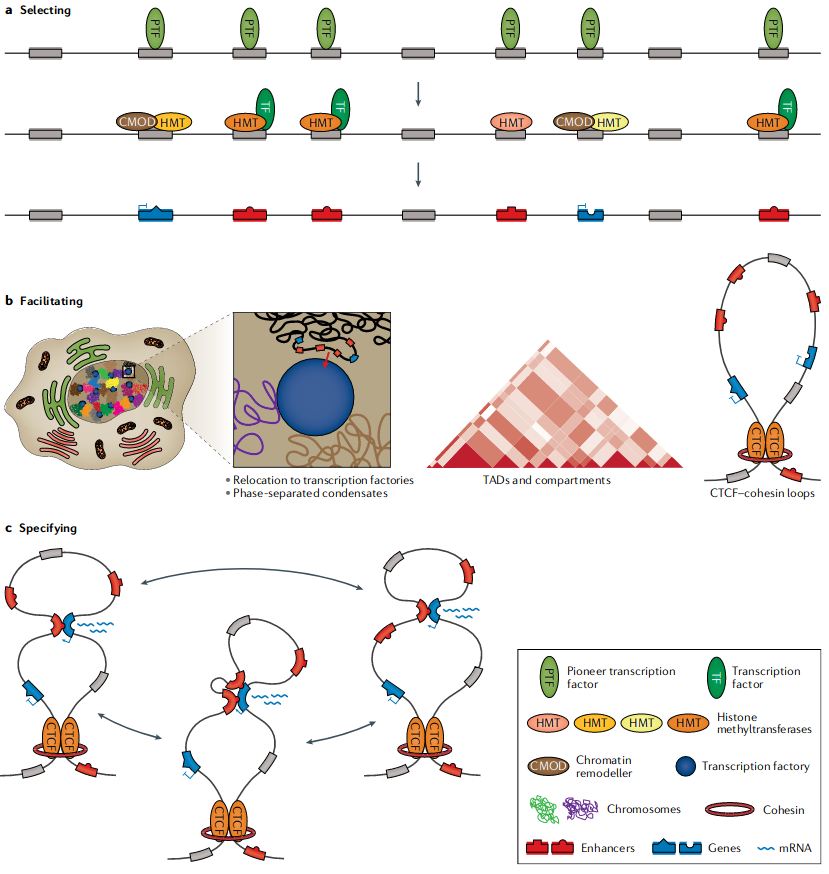
\includegraphics[width=0.8\textwidth, page=1] {figures/introduction/fig14.png}
 \caption[Modèle de sélection, facilitation, spécificité pour les contacts entre promoteur et amplificateur.]{
 \textbf{Modèle de sélection, facilitation, spécificité pour les contacts entre promoteur et amplificateur.}
 \textbf{A.} La \textbf{sélection} : l'action combinée des facteurs de transcription pionniers, des enzymes de remodelage de la chromatine, des facteurs de transcription et des enzymes de modification de la chromatine, telles que les histones méthyltransférases, marque les éléments \textit{cis}-régulateurs spécifiques du type cellulaire par des modifications épigénétiques et la création de sites de liaison pour les protéines de la chromatine. \textbf{B.} La \textbf{facilitation}. La relocalisation de régions génomiques dans des usines de transcription, des domaines d'association topologique (TAD), des compartiments et des boucles créent des micro-environnements qui réduisent l'espace de recherche et augmentent ainsi les chances de rencontre entre les éléments \textit{cis}-régulateurs dans l'espace tridimensionnel. \textbf{C.} La \textbf{spécificité} du contact entre les \glspl{amplificateur} et les promoteurs au sein des domaines ou des boucles est obtenue par des interactions entre facteurs de transcription et éléments \textit{cis}-régulateurs. Ceci permet des transitions dynamiques entre les conformations.
 Tiré de \citet{schoenfelder_long-range_2019}.\\
 }
 \label{fig:Fig14}
\end{figure}


\subsubsection{Contacts spécifiques et préformation}
\label{subsubsec:specifique-preformation}

La mise en place de contacts spécifiques de la chromatine dans les différentes cellules pour permettre leur spécialisation est encore mal comprise. La comparaison de la conformation de la chromatine entre plusieurs types cellulaires d’une même espèce a montré qu’une grande proportion (autour de 40\%) des contacts est spécifique du type cellulaire \citep{javierre_lineage-specific_2016}. Malgré une importante spécialisation, de nombreux contacts sont cependant conservés au cours de la différenciation et sont partagés entre les types cellulaires et plus de 10\% d'entre eux seraient constitutifs  \citep{freire-pritchett_global_2017, rubin_lineage-specific_2017}. Il a également été montré que le regroupement de différentes cellules du sang selon la similarité de leurs contacts reflète les relations de proximité des cellules au cours de la différenciation de la lignée hématopoïétique \citep{javierre_lineage-specific_2016}. Il en va de même pour la spécialisation des cellules de la lignée épidermique \citep{rubin_lineage-specific_2017}. Ces observations suggèrent que les contacts de chromatine changent progressivement au cours de la différenciation cellulaire à partir d'un état précurseur dans les cellules souches. \\

Certains contacts observés dans un type cellulaire donné mettent en relation des éléments \glspl{amplificateur} de l’expression avec des gènes qui ne sont pas actifs dans ce type cellulaire \citep{schoenfelder_pluripotent_2015}. Par exemple, les \glspl{amplificateur} sensibles au facteur de nécrose tumorale dans les fibroblastes humains sont déjà en contact avec les promoteurs des gènes cibles avant la signalisation par ce facteur \citep{jin_high-resolution_2013}. Ces contacts dits pré-formés sont présents avant la transcription des gènes cibles qui s’effectue seulement en réponse à d’autres stimuli. La proximité spatiale entre promoteur et \gls{amplificateur} n’induit donc pas automatiquement une activation du gène, mais pourrait permettre une réponse transcriptionnelle rapide et précise avec l’action combinée d’autres déclencheurs. Les cas de pré-formation de contact de chromatine ne se limitent pas à des voies de signalisation rapides. Le contact entre \acrshort{SHH} et son \gls{amplificateur} \acrshort{ZRS} par exemple a été observé dans de nombreux tissus sans que le gène ne soit exprimé \citep{amano_chromosomal_2009, williamson_shh_2016, ron_promoter-enhancer_2017}. La pré-formation dans ce cas pourrait assurer une proximité constante pour permettre un patron d’expression robuste de \acrshort{SHH} lorsque le gène doit être actif \citep{paliou_preformed_2019}. Plus généralement les contacts pré-formés pourraient maintenir les relations \gls{cis}-régulatrices ayant des impacts majeurs sur le développement ou la survie des individus. 

\subsection{Techniques d’identification des contacts}
\label{subsec:contact-identification}

Identifier la présence de boucles d’ADN et plus généralement la conformation tridimensionnelle de l’ensemble du génome reste encore un défi. De nombreuses avancées et techniques biomoléculaires ont permis d’avoir un aperçu de l’organisation spatiale du génome. Je vais décrire ici quelques-unes de ces techniques et ce qu’elles ont permis de révéler sur l’organisation du génome.

\subsection{Microscopie et cytogénétique moléculaire}
\label{subsec:microscopie}

Les premières observations de l’organisation spatiale du génome ont été rendues possibles par des techniques de microscopie électronique et de cytogénétique moléculaire. Étant très éloigné de ces domaines je ne m'étendrai pas longuement sur celles-ci. Cependant elles ont permis dès le début des années 90 d’observer les premières boucles d’ADN sur des plasmides bactériens entre un facteur de transcription fixé sur la séquence d’un \gls{amplificateur} et l’ARN polymérase II fixée sur le promoteur d’un gène \citep{su_dna-looping_1990}. Une colocalisation spatiale entre \acrshort{SHH} et l’\gls{amplificateur} \acrshort{ZRS} a également pu être observée grâce à un marquage fluorescent par hybridation \textit{in situ} (FISH) au niveau de la séquence de \acrshort{ZRS} et du promoteur de \acrshort{SHH} (Figure \ref{fig:fig15-17}.A-B), \citep{amano_chromosomal_2009}. Plus récemment, des techniques de microscopie avancées comme la microscopie en super-résolution, ont révélé que \acrshort{SHH} et \acrshort{ZRS} sont spatialement proches dans de nombreux tissus mais que la distance entre les deux loci est la plus faible dans la zone d’activité de polarisation durant le développement des membres \citep{williamson_shh_2016}. Finalement, des techniques de microscopie sur cellules vivantes permettent aujourd’hui de visualiser les contacts entre des loci cibles marqués par fluorescence, tout en suivant l’activité de gènes rapporteurs de l’expression en temps réel (Figure \ref{fig:fig15-17}.D). Une étude récente a ainsi montré que la colocalisation entre l’\gls{amplificateur} EVE et le promoteur du gène cible \textit{PP7} corrèle avec l’activité de ce gène dans des cellules de drosophile. La distance entre les deux loci est significativement plus faible lorsque le gène est actif (Figure \ref{fig:fig15-17}.C) \citep{chen_dynamic_2018}. \\

\begin{figure}[h]
 \centering
 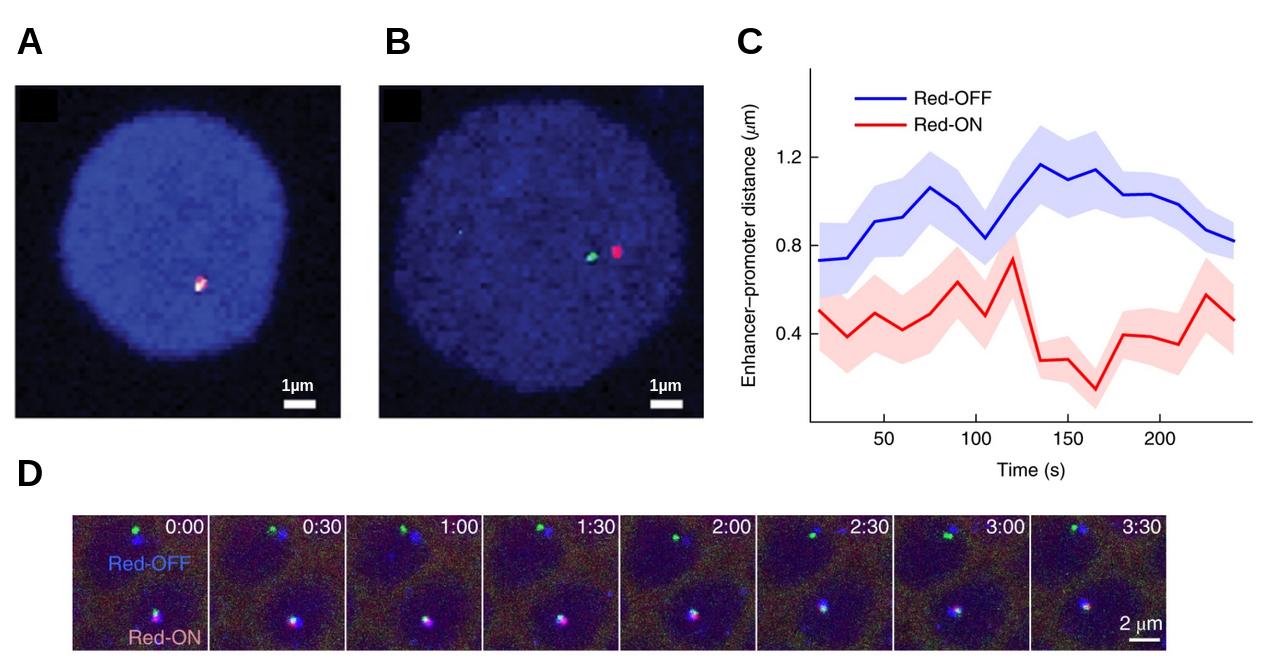
\includegraphics[width=1\textwidth, page=1] {figures/introduction/fig15-17.png}
 \caption[Colocalisation entre gène et \gls{amplificateur} observé par microscopie.]{
 \textbf{Colocalisation entre gène et \gls{amplificateur} observé par microscopie.}
 \textbf{A.} Colocalisation de \acrshort{SHH} et de \acrshort{ZRS} marqués en fluorescence par hybridation \textit{in situ} (FISH) dans des cellules de bourgeons de membres au sein d'un embryon de souris au jour 10.5.
 \textbf{B.} Dans certaines cellules, les deux loci peuvent être séparés.
 \textbf{C.} Suivi temporel de la distance spatiale entre l'\gls{amplificateur} EVE et le promoteur du gène \textit{PP7} dans deux cellules de drosophile lorsque \textit{PP7} est actif (Red-ON) ou inactif (Red-OFF).
 \textbf{D.} 8 photographies suivant 2 noyaux pendant 3min30 où la séquence de EVE (bleue) et le promoteur de \textit{PP7} (vert) sont marqués par FISH. Le noyau en bas présente une activité du gène \textit{PP7} dont les transcrits sont colorés en rouge (Red-ON), alors que dans celui du haut le gène n'est pas actif (Red-OFF).
 Tiréees de \citet{amano_chromosomal_2009} et de \citet{chen_dynamic_2018}.\\
 }
 \label{fig:fig15-17}
\end{figure}

De telles observations ont permis de confirmer un mécanisme de régulation en \gls{cis} par le rapprochement physique des promoteurs et des \glspl{amplificateur} séparés par de grandes régions génomiques. Elles sont essentielles à la compréhension de la dynamique spatiale des génomes.

\subsection{Capture de la conformation de la chromatine}
\label{subsec:HiC}

Ces vingt dernières années, des méthodes expérimentales ont été mises au point pour analyser et prédire plus finement mais aussi de manière plus systématique les contacts de chromatine, et parmi eux les interactions entre gènes et éléments \gls{cis}-régulateurs \citep{dekker_capturing_2002, simonis_nuclear_2006, dostie_chromosome_2006, lieberman-aiden_comprehensive_2009,schoenfelder_pluripotent_2015}. \\

La principale approche expérimentale pour identifier les contacts entre deux loci génomiques est basée sur la liaison par proximité spatiale. Cette approche fait partie des méthodes dites de Capture de Conformation de Chromosome (\acrshort{3C}) (voir \citet{han_3c_2018} pour une revue des méthodes). Elles permettent d’isoler et de séquencer des régions d’ADN se trouvant à proximité spatiale dans le noyau des cellules. En fonction des méthodes de \acrshort{3C} employées, différents contacts entre des loci peuvent être identifiés. On peut les regrouper en quatre grandes classes : un-à-un (analyse du contact entre deux loci ciblés : \acrshort{3C} classique), un-à-tous (analyse de tous les contacts d’un locus cible : \acrshort{3C}-on-Chip, Circular-\acrshort{3C} ou 4C), plusieurs-à-plusieurs (analyse des contacts entre plusieurs loci ciblés : \acrshort{3C}-Carbon-Copy ou 5C) et tous-à-tous (ensemble des contacts à l’échelle du génome : High-throughput-\acrshort{3C} ou \acrshort{Hi-C}) \citep{han_3c_2018}.\\

\begin{figure}[h]
 \centering
 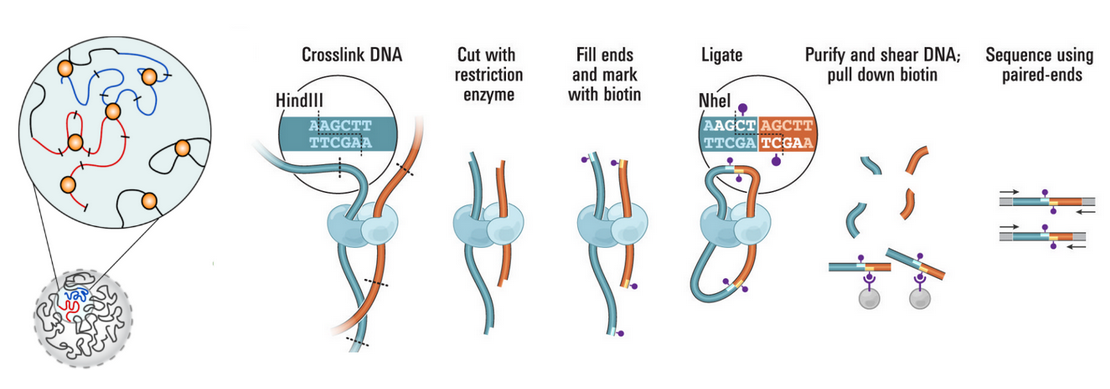
\includegraphics[width=1\textwidth, page=1] {figures/introduction/fig18.png}
 \caption[Principe de capture de la conformation de la chromatine par Hi-C.]{
 \textbf{Principe de capture de la conformation de la chromatine par Hi-C.}
 La conformation de l'ADN dans le noyau des cellules est fixée avec du formaldéhyde, les segments de chromatine proches (représentés en bleu et rouge) sont ainsi liés. Les protéines qui lient les fragments d'ADN sont représentées en bleu clair. La chromatine est ensuite coupée par une enzyme de restriction (HindIII ici) et les extrémités de l'ADN sont marquées par la biotine (ronds violets). Les extrémités sont ensuite liées créant des molécules chimériques. L'ADN est purifié, puis les jonctions biotinylées sont isolées et identifiées par séquençage. Tirée de \citet{lieberman-aiden_comprehensive_2009}.\\
 }
 \label{fig:Fig18}
\end{figure}

Les méthodes de type \acrshort{3C} sont basées sur la fixation au formaldéhyde de la conformation de l’ADN dans le noyau à un instant donné dans le but de figer la chromatine (Figure \ref{fig:Fig18}). Le formaldéhyde entraîne une liaison chimique qui fixe entre eux les loci génomiques qui se trouvent à proximité physique dans le noyau. S'ensuit une étape de digestion de l’ADN par une enzyme de restriction comme HindIII qui reconnaît des sites spécifiques et qui découpe le génome en plusieurs centaines de milliers de fragments de 4 kilobases en moyenne chez l’humain ou la souris. Dans le cas du \acrshort{Hi-C}, chaque extrémité des fragments génomiques est marquée par une biotine. Les fragments découpés sont ensuite ligués de façon circulaire par l’enzyme Nhel, dont les sites de restriction sont en partie communs à ceux de HindIII. Ces fragments circulaires vont alors être purifiés, puis subir des découpes aléatoires par sonication. \`A cette étape, selon la méthode utilisée, différents fragments sont filtrés. Soit sont sélectionnés les fragments contenant les loci ciblés (\acrshort{3C}, 4C, 5C), soit dans le cas du \acrshort{Hi-C}, toutes les séquences contenant des biotines, c’est-à-dire les jointures entre deux fragments de restriction ligués \citep{lieberman-aiden_comprehensive_2009}. Les séquences sélectionnées sont alors amplifiées par PCR puis séquencées à haut débit. La fréquence d'une séquence contenant une partie de deux fragments distincts est ainsi une mesure de la fréquence à laquelle, dans une population cellulaire, les fragments se trouvaient à proximité immédiate au moment de la fixation. \\


La grande limitation du \acrshort{Hi-C} reste la puissance de séquençage. Si l’utilisation de la biotine pour séquencer uniquement les fragments dérivant de contacts de chromatine permet en théorie d’isoler et d’identifier l’ensemble des interactions chromosomiques d’une population de cellules, le nombre de combinaisons possibles est énorme. Les bibliothèques \acrshort{Hi-C}, généralement générées à partir de millions de cellules, sont extrêmement complexes et peuvent représenter près de 100 milliards de séquences indépendantes représentant les jointures de fragments génomiques \citep{belton_hic_2012}. Des méthodes dites de Capture-\acrshort{Hi-C} ont été développées pour traiter et enrichir uniquement un sous-échantillon de ces jointures. Plusieurs techniques d’isolation des interactions existent, certaines combinent les approches C avec une immunoprécipitation de la chromatine pour cibler des fragments contenant des protéines spécifiques, c’est le cas des Chia-Pet ou HiChiP \citep{fullwood_chip-based_2009}. Au cours de ma thèse j’ai utilisé des données produites par une autre approche qui vise à enrichir spécifiquement les jointures obtenus en \acrshort{Hi-C} qui contiennent des promoteurs de gènes, nommée Promoter-Capture-\acrshort{Hi-C} (\acrshort{PCHi-C}) \citep{schoenfelder_pluripotent_2015}. Dans cette approche, des amorces spécifiques sont construites pour s’hybrider par complémentarité avec les extrémités des fragments contenant des promoteurs (près de 40,000 fragments contenant plus de 20,000 promoteurs de gènes pour le génome humain). Ainsi, avant le séquençage, une étape supplémentaire est introduite pour filtrer et amplifier par PCR seulement les jointures faisant intervenir les fragments ciblés. Cette étape de sélection est cruciale car la profondeur de séquençage est limitée, et le signal permettant de détecter une interaction chromosomique peut être entièrement noyé par les interactions les plus fréquentes, abaissant ainsi la sensibilité totale (Figure \ref{fig:Fig19}). Grâce à la technique de \acrshort{PCHi-C}, des catalogues de contacts entre promoteurs des gènes et autres régions génomiques (potentiellement régulatrices) sont disponibles pour plusieurs types cellulaires pour l’humain et la souris. Ils permettent une prédiction expérimentale des relations \gls{cis}-régulatrices à l’échelle du génome complet. De telles données ont ainsi permis de confirmer que le promoteur de \acrshort{SHH} est situé à proximité spatiale de l’\gls{amplificateur} dans plusieurs types cellulaires \acrshort{ZRS} \citep{javierre_lineage-specific_2016, laverre_long-range_2022}. \\

\begin{figure}[h]
 \centering
 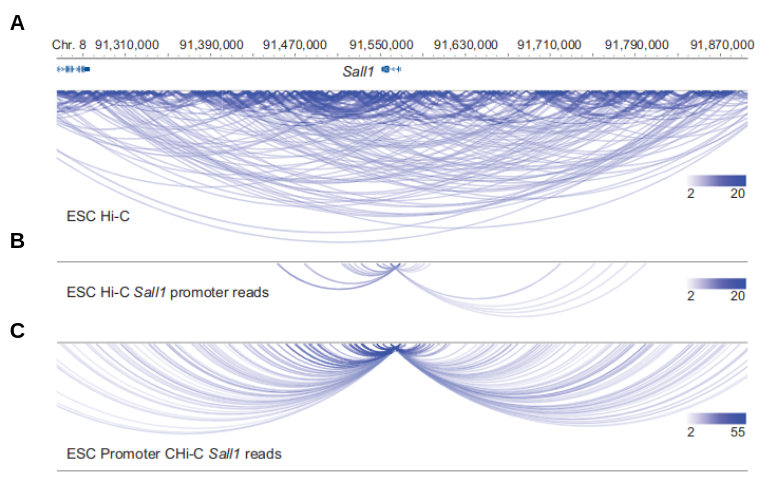
\includegraphics[width=0.8\textwidth, page=1] {figures/introduction/fig19.png}
 \caption[Comparaison des contacts de la chromatine mesurés par \acrshort{Hi-C} et par \acrshort{PCHi-C}.]{
 \textbf{Comparaison des contacts de la chromatine mesurés par \acrshort{Hi-C} et par \acrshort{PCHi-C}.}
 \textbf{A.} Interactions détectées en \acrshort{Hi-C} dans une région de 0.6Mb contenant le gène \textit{Sall1} dans les cellules souches humaines. L'intensité de la couleur d'une interaction indique le nombre de paires de lectures de séquençage entre deux séquences contactées. \textbf{B.} Même expérience de \acrshort{Hi-C}, mais seules les interactions qui mettent en contact le promoteur du gène \textit{Sall1} sont montrées. \textbf{C.} Interactions détectées en \acrshort{PCHi-C}qui contactent le promoteur de \textit{Sall1}. Le nombre de paires de lectures sur l'ensemble de l'échantillon a été ajusté pour être équivalent entre \acrshort{Hi-C} et \acrshort{PCHi-C}. Tirée de \citet{schoenfelder_pluripotent_2015}.\\
 }
 \label{fig:Fig19}
\end{figure}


\section{Le paysage \textit{cis}-régulateur}
\label{sec:paysage-cis-regul}

Afin de comprendre les déterminants de l'expression d'un gène il est alors important de pouvoir décrire l'ensemble de ses relations \gls{cis}-régulatrices. Les études qui se sont attachées à décrire ces relations ont alors fait émerger la notion de paysage \textit{cis}-régulateur de l'expression.

\subsection{Evolution de la définition du paysage \textit{cis}-régulateur}
\label{subsec:evol-def}

Ce terme de paysage a d’abord vu le jour à partir de l’observation de la structure hétérogène de la chromatine : les différences de compaction de l’ADN le long du génome ainsi que la variabilité des marques épigénétiques ont permis de définir un “paysage de chromatine” associé à l’activité des gènes \citep{grewal_heterochromatin_2003}. Un tel paysage ne permet pas à lui seul de décrire les relations régulatrices entre les gènes et les éléments \gls{cis}-régulateurs. Cependant il définit des grandes régions génomiques où la chromatine est dans un état qui permet ou pas l’expression des gènes. \\

Un autre type de paysage régulateur de l’expression des gènes a ensuite été défini à partir de la découverte de régions génomiques contenant plusieurs \glspl{amplificateur} régulant des gènes co-exprimés voisins \citep{spitz_global_2003}. Certains gènes agissent de manière coordonnée, par exemple pour former des complexes multi-protéines ou alors pour fonctionner dans les mêmes voies métaboliques. Ils peuvent être co-régulés par des éléments \gls{cis}-régulateurs communs et être regroupés dans une région génomique restreinte. C’est par exemple le cas des gènes \textit{HOX} qui sont responsables de nombreux processus développementaux, et qui sont regroupés dans certaines régions génomiques et peuvent être régulés par des \glspl{amplificateur} distaux communs \citep{spitz_global_2008}. D’après ces observations sur les gènes co-régulés, le paysage régulateur représenterait l’intervalle d’ADN à l’intérieur duquel l'ensemble des gènes est sous l’influence d’une même région régulatrice (Figure \ref{fig:Fig20}) \citep{spitz_global_2003}. Avec cette définition, la taille d’un paysage régulateur peut être variable selon le nombre d’éléments \gls{cis}-régulateurs y étant présents et selon les types cellulaires. \\

\begin{figure}[h]
 \centering
 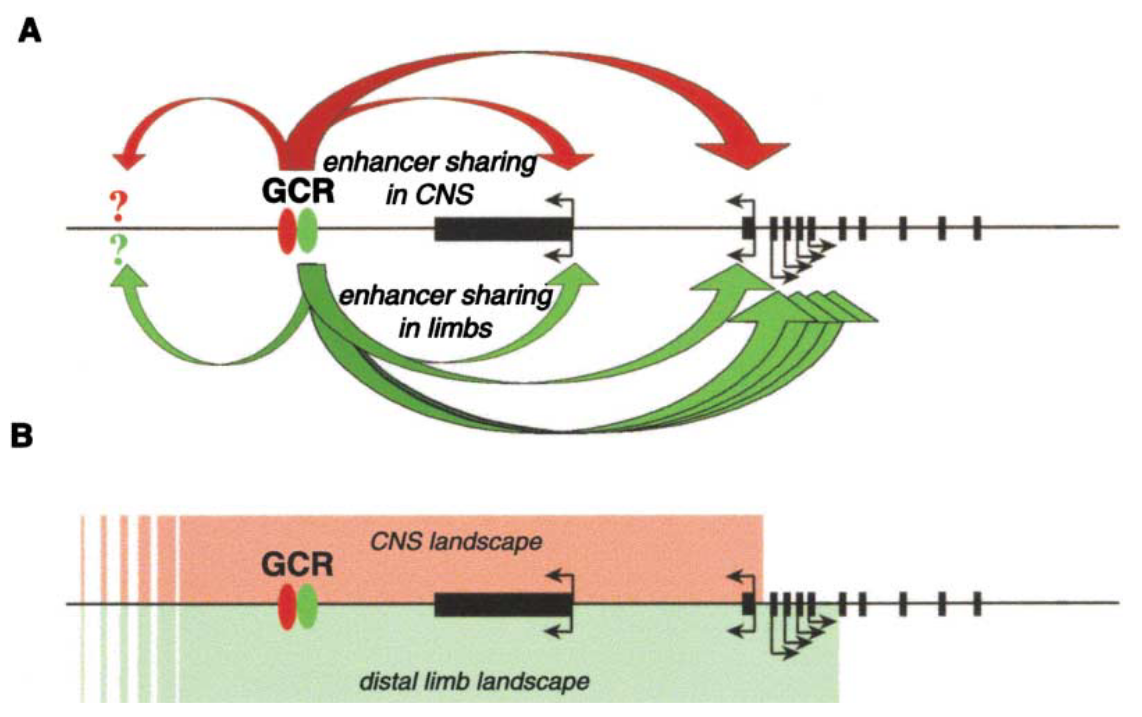
\includegraphics[width=0.8\textwidth, page=1] {figures/introduction/fig20.png}
 \caption[Première vision d'un paysage \gls{cis}-régulateur.]{
 \textbf{Première vision d'un paysage \gls{cis}-régulateur.}
 \textbf{A.} Une région riche en \glspl{amplificateur} (GCR pour global control region) peut contrôler l'expression de plusieurs gènes distants co-actifs. L'influence de cette région peut être variable selon les types cellulaires, en rouge co-activation des gènes dans le système nerveux central (CNS), en vert co-activation d'un plus grand nombre de gènes dans le développement des membres. \textbf{B.} Selon les types cellulaires, les frontières du paysages régulateurs pourraient donc être différentes. Tirée de \citet{spitz_global_2003}.\\
 }
 \label{fig:Fig20}
\end{figure}

De nombreux éléments \gls{cis}-régulateurs sont localisés tels des îlots dans les déserts de gènes autour des regroupements de gènes \textit{HOX} (Figure \ref{fig:Fig21}.A) \citep{montavon_regulatory_2011}. L’étude de l’organisation spatiale de la chromatine a révélé que certains de ces éléments \gls{cis}-régulateurs sont amenés de manière indépendante ou simultanée au voisinage du gène \textit{Hoxd13} par des boucles d’ADN \citep{montavon_regulatory_2011}. Ces interactions permettent une robustesse de l’expression de \textit{Hoxd13} tout en affinant de manière spécifique son activité dans plusieurs contextes distincts. Dans l'étude de Montavon et collaborateurs, les paysages régulateurs deviennent alors des ”archipels régulateurs” où les gènes peuvent être en interaction avec différents îlots  d’éléments \gls{cis}-régulateurs indépendants. \\

\begin{figure}[h]
 \centering
 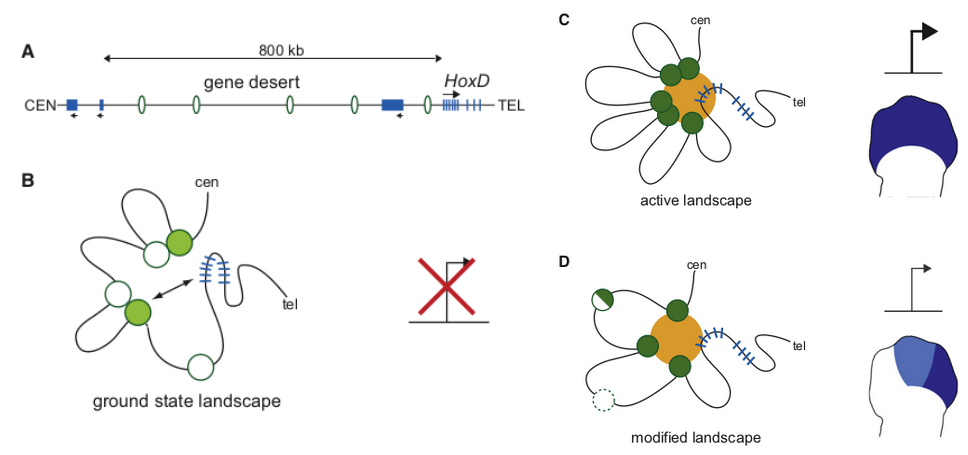
\includegraphics[width=1\textwidth, page=1] {figures/introduction/fig21.png}
 \caption[Notion d'archipel régulateur.]{
 \textbf{Notion d'archipel régulateur.}
 \textbf{A.} Segment génomique représentant un désert de gène dans une région de 800kb autour du promoteur de \textit{HoxD13}. Les rectangles bleus représentent des gènes et les cercles verts des îlots d'éléments \gls{cis}-régulateurs. \textbf{B.} Représentation de la conformation de la chromatine lorsque le gène \textit{HoxD13} n'est pas exprimé. Certains îlots possèdent des marques épigénétiques d'\glspl{amplificateur} actifs (rond vert plein) et peuvent contacter le promoteur du gène mais ne suffisent pas à initier sa transcription. \textbf{C.} \textit{HoxD13} est en contact avec l'ensemble des îlots actifs, il est exprimé de manière homogène dans le tissu. \textbf{D.} \textit{HoxD13} est en contact avec une partie des îlots et présente un patron d'activité différente. Tirée de \citet{montavon_regulatory_2011}. \\
 }
 \label{fig:Fig21}
\end{figure}

La définition de paysage \gls{cis}-régulateur évolue ensuite avec l’accumulation d’exemples de relations régulatrices à grande distance entre des promoteurs et des éléments \gls{cis}-régulateurs \citep{montavon_landscapes_2012}. Des cas comme celui de \acrshort{SHH} et \acrshort{ZRS} où la régulation s’effectue à très grande distance génomique, outre-passant plusieurs gènes, et n'activant aucun autre gène voisin, permettent d’en savoir plus sur les modes d’action des éléments \gls{cis}-régulateurs. C’est grâce au développement récent des techniques de capture de conformation de la chromatine (notamment les approches de types \acrshort{Hi-C}) que les paysages \gls{cis}-régulateurs peuvent aujourd’hui être mieux décrits et investigués à l’échelle du génome complet. \\

Au cours de cette thèse, je définirai donc le paysage \gls{cis}-régulateur d’un gène comme l’ensemble des éléments \gls{cis}-régulateurs qui peuvent avoir un impact sur le niveau ou l’étendue de son expression. Cette définition évoque un paysage complexe à déterminer : les sous-ensembles d’éléments \gls{cis}-régulateurs d’un gène peuvent être différents selon l’étape de division cellulaire, le stade de développement, le type cellulaire, les facteurs environnementaux, etc.. Il apparaît ambitieux d’avoir une mesure ou une connaissance exhaustive du paysage \gls{cis}-régulateur d’un gène. Cependant la multiplication des expériences, notamment par des mesures des contacts de chromatine, dans un grand nombre de contextes permet d’en obtenir un aperçu.

\subsection{Complexité du paysage \textit{cis}-régulateur et patron d’expression des gènes}
\label{subsec:complexite}

Les paysages \gls{cis}-régulateurs de l’expression des gènes peuvent mettre en relation de nombreuses séquences fonctionnelles. Chaque gène peut en effet être associé à plusieurs éléments \gls{cis}-régulateurs et inversement chaque élément peut contrôler plusieurs gènes. Ces associations peuvent se faire de manière simultanée par des boucles de la chromatine qui co-localisent plusieurs éléments. Par exemple, il a été montré qu’un \gls{amplificateur} peut réguler simultanément deux gènes distants l’un de l’autre sur le génome linéaire \citep{fukaya_enhancer_2016}. Plusieurs \glspl{amplificateur} peuvent être nécessaires pour activer la transcription d’un gène, en recrutant différents facteurs de régulation en \gls{trans} par exemple. Les \glspl{amplificateur} peuvent également avoir des fonctions partiellement ou totalement redondantes sur l’expression des gènes cibles. Cette redondance pourrait assurer une robustesse de l’expression des gènes cibles \citep{berthelot_complexity_2018}. En augmentant le nombre d’\glspl{amplificateur}, la probabilité de rencontre entre un gène et un \gls{amplificateur} est en effet augmentée, ce qui augmente les chances que la transcription soit initiée. De plus, il a été montré que le nombre d’\glspl{amplificateur} avec lequel un gène interagit est corrélé positivement avec son niveau d’expression \citep{schoenfelder_pluripotent_2015, mifsud_mapping_2015, javierre_lineage-specific_2016, berthelot_complexity_2018}. Ceci suggère un effet additif des \glspl{amplificateur} qui permettraient une augmentation de la fréquence des cycles d’activité de la transcription du gène \citep{bartman_enhancer_2016}. Certains \glspl{amplificateur} ont cependant des fonctions non redondantes et sont obligatoires pour assurer la transcription du gène dans un contexte donné. \\

\begin{figure}[hbt!]
 \centering
 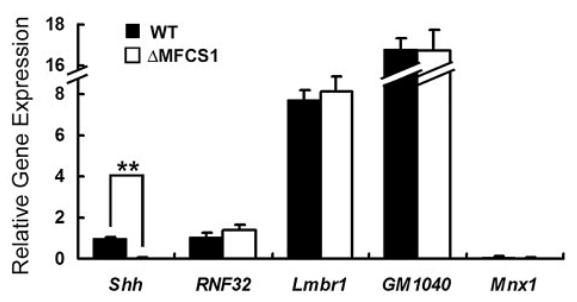
\includegraphics[width=0.7\textwidth, page=1] {figures/introduction/fig22.png}
 \caption[Impact de la délétion de \acrshort{ZRS} sur l'expression de ces quatre gènes voisins et du gène \acrshort{SHH} distal.]{
 \textbf{Impact de la délétion de \acrshort{ZRS} sur l'expression de ces quatre gènes voisins et du gène \acrshort{SHH} distal.}
 Expression relative des gènes dans le bourgeon des membres inférieurs d'embryon de souris avec un génotype sauvage (noir) ou étant homozygotes pour la délétion de \acrshort{ZRS} (précédemment nommé MFCS1) (blanc). Les niveaux d'expression des gènes sont normalisés par le niveau d'expression du gène de ménage de la Beta-actine. Le niveau d'expression de \acrshort{SHH} dans l'embryon sauvage est pris comme référence. Les barres d'erreur représentent les écarts types obtenus à partir des expériences réalisées sur trois réplicats. Les doubles astérisques indiquent des différences significatives, évaluées par le test t de Welch (p $<$ 0,01).Tirée de \citet{amano_chromosomal_2009}.\\
 }
 \label{fig:Fig22}
\end{figure}

Un élément \gls{cis}-régulateur peut réguler l’expression de plusieurs gènes en même temps et/ou dans des types cellulaires différents, et ainsi avoir de nombreuses fonctions. Les \glspl{amplificateur} seraient majoritairement spécifiques d’un tissu, indépendamment des gènes qu’ils régulent \citep{singh_enhancer_2021}. Certains \glspl{amplificateur} sont en effet très spécifiques comme c’est le cas de \acrshort{ZRS} qui semble réguler uniquement \acrshort{SHH} et uniquement dans le développement des membres. La délétion de celui-ci dans le génome de la souris réduit significativement l’expression de \acrshort{SHH} sans affecter l'expression des quatre gènes avoisinant \acrshort{ZRS} (Figure \ref{fig:Fig22}) \citep{amano_chromosomal_2009}. Il est cependant difficile d’estimer précisément l’ensemble des gènes cibles d’un \gls{amplificateur}. Bien que cela n'ait pas été testé, \acrshort{ZRS} pourrait par exemple affecter d’autres gènes plus distaux ou des gènes dans des contextes cellulaires différents. Le gène \acrshort{SHH} est cependant très \gls{pleiotrope} et assure différentes fonctions dans plusieurs types cellulaires. L’expression de \acrshort{SHH} est régulée par plusieurs \glspl{amplificateur} spécifiques de différents tissus et situés dans une large région s’étendant à plus de 1Mb autour du gène \citep{epstein_regionalization_1999, lettice_long-range_2003}. \\

C’est donc l’interaction modulable des éléments \gls{cis}-régulateurs avec un gène cible, conjointement avec l’état de la chromatine et la présence de facteurs agissant en \gls{trans}, qui permet d’établir son patron d’expression pour chaque type cellulaire (Figure \ref{fig:Fig23}). Le paysage \gls{cis}-régulateur permet d’affiner précisément le patron d’expression d’un gène dans chaque type cellulaire. De par la possible complexité du paysage \gls{cis}-régulateur d'un gène, une importante modularité des éléments \gls{cis}-régulateurs est possible. C'est-à-dire que différentes configurations à partir d'un même ensemble d'élements \gls{cis}-régulateurs pourrait permettre aux gènes d’être actifs dans un plus grand nombre de types cellulaires et d’être impliqués dans un plus grand nombre de fonctions métaboliques. Finalement, la redondance d’un tel réseau de régulation peut permettre une plus grande tolérance aux mutations et serait alors en mesure de participer à une forte plasticité et évolution de l’expression des gènes.

\begin{figure}[h]
 \centering
 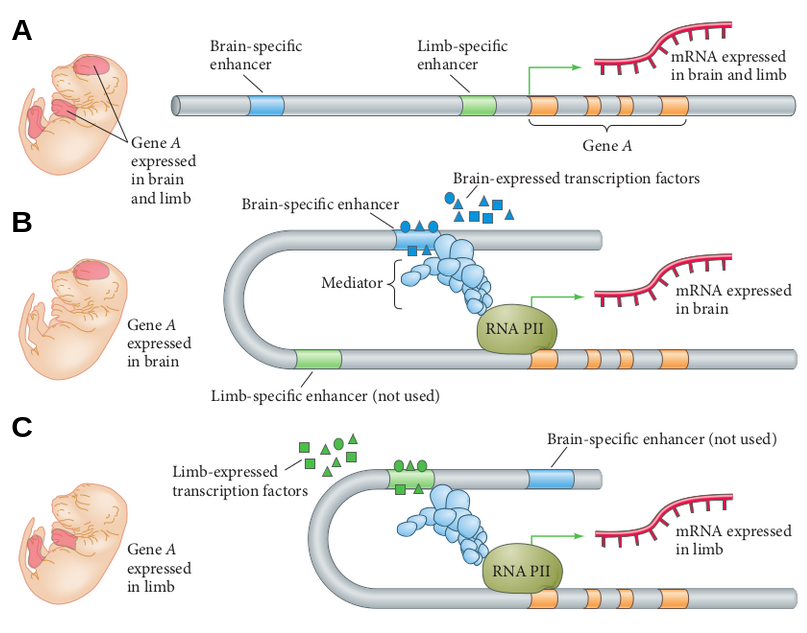
\includegraphics[width=0.9\textwidth, page=1] {figures/introduction/fig23.png}
 \caption[Modularité du paysage \gls{cis}-régulateur.]{
 \textbf{Modularité du paysage \gls{cis}-régulateur.}
 \textbf{A.} Schéma modèle d'un gène A, composé de 4 exons (orange), exprimé dans le cerveau et les membres au cours du développement. Son paysage \gls{cis}-régulateur est composé d'au moins deux \glspl{amplificateur} : l'un spécifique du cerveau (bleu) un autre des membres (vert). 
 \textbf{B.} Dans le cerveau, des facteurs de transcription se fixent sur l'\gls{amplificateur} spécifique. Ceci permet de recruter diverses protéines qui vont changer la structure de la chromatine et recruter l'\acrshort{ARN} polymérase II pour transcrire le gène A. L'\gls{amplificateur} spécifique des membres n'est pas utilisé, par exemple à cause de modification épigénétique particulière ou d'absence d'éléments \gls{trans}-régulateurs spécifiques de sa séquence.
 \textbf{C.} Scénario similaire dans les membres, où le gène A est transcrit grâce à l'\gls{amplificateur} spécifique de ce tissu. Le gène n'est pas activé dans d'autres \glspl{condition} où les facteurs de transcription ne peuvent se lier à l'un de ces deux \glspl{amplificateur}.
 Tiré de \citet{gilbert_developmental_2017}.
 }
 \label{fig:Fig23}
\end{figure}


    \chapter{Un regard évolutif}
{\hypersetup{linkcolor=GREYDARK}\minitoc}
\label{chap:evolution}

\section{Évolution de l’expression des gènes}
\label{sec:evolution-gene}

Une grande partie de la variation observée entre individus en termes de niveaux d'expression des gènes est héritable et a souvent une base génétique \citep{emilsson_genetics_2008,aguet_genetic_2017}. En raison de son impact sur les phénotypes morphologiques et physiologiques, l’expression des gènes peut alors être considérée comme un phénotype moléculaire intermédiaire.

\subsection{Un modèle d’évolution quasi-neutre pour l’expression des gènes}
\label{subsec:modele-neutre}

Afin d’interpréter les résultats des études comparatives de l’expression des gènes entre espèces et d’en inférer des scénarios évolutifs, il est important de déterminer si les différences observées sont le résultat de la sélection naturelle ou de processus stochastiques. La sélection naturelle joue un rôle majeur en filtrant les organismes les mieux adaptés à leur environnement. La sélection naturelle agit seulement à l’échelle des phénotypes alors que la variation est générée à l’échelle du génotype. Toutes les mutations n'entraînent pas des modifications phénotypiques, et on peut donc s’attendre à ce que la proportion des changements sélectifs décroisse graduellement à mesure que l’on s’éloigne du phénotype. Kimura a ainsi proposé que la grande majorité des différences observées entre les génomes des espèces n’affectent pas ou très peu les phénotypes des organismes, elles n’ont pas d’impact sur la valeur sélective des individus et sont donc neutres \citep{kimura_neutral_1983}. D’après un modèle quasi-neutre d’évolution moléculaire initié par Kimura et complété par Ohta, la majorité des mutations seraient soit délétères et éliminées par la sélection naturelle dite alors purifiante, soit faiblement délétères et ségrègeraient alors dans les génomes par dérive génétique \citep{ohta_synonymous_1995}. La probabilité de fixation d’une mutation faiblement délétère dépend de son impact sur la survie et la reproduction d’un individu. Cet impact est mesuré par un coefficient de sélection et dépend de la taille efficace de la population \citep{charlesworth_effective_2009}. Une population avec un plus grand nombre d’individus reproducteurs est en mesure de filtrer plus efficacement les mutations ayant un faible coefficient de sélection \citep{ohta_slightly_1973}. Les mutations arriveraient à fixation soit par dérive génétique, soit beaucoup plus rarement par sélection positive lorsque la mutation présente un avantage suffisant pour l’individu. Ce modèle implique que la majorité des différences entre les espèces est déterminée par des processus non adaptatifs comme la mutation et la dérive génétique. \\

Est-il possible d’utiliser ce modèle quasi-neutre d’évolution moléculaire, développé pour décrire la divergence des séquences, pour proposer un modèle nul de l'évolution de l’expression des gènes ? On s'attendrait alors à ce que le taux d’évolution du niveau d’expression soit fortement dépendant du taux de mutation, de la taille de la population et des contraintes agissant sur le niveau d’expression du gène. Dans le cas d’une évolution dominée par des processus non adaptatifs, les différences entre les espèces devraient s’accumuler de manière approximativement linéaire avec le temps de divergence. De plus, la variation de l’expression d’un gène entre espèces devrait être liée à la variation de l’expression de ce gène dans une population. Les écarts à ces prédictions de l’hypothèse nulle pourraient alors permettre de détecter des changements adaptatifs de l’expression des gènes.\\

Khaitovich et ses collaborateurs ont tenté de tester ces prédictions pour l’évolution de l’expression en décrivant les différences dans les \glspl{transcriptome} de plusieurs espèces proches de primates \citep{khaitovich_neutral_2004}. Premièrement, ils ont observé que l’accumulation de différences du niveau d’expression d’environ 12 000 gènes dans le cortex préfrontal est effectivement linéaire avec le temps de divergence entre les paires d’espèces (Figure \ref{fig:Fig24}.A). Autrement dit, les variations des niveaux d’expression des gènes reflètent les relations phylogénétiques selon un principe d’horloge moléculaire, ce qui confirme la première prédiction d’un modèle quasi-neutre. Ils ont ensuite comparé la divergence inter-espèces du niveau d’expression des gènes ayant le plus et le moins de variations intra-espèces (Figure \ref{fig:Fig24}.B). Les gènes ayant le plus de variations chez l’humain accumulent des différences entre espèces significativement plus rapidement que les autres, ce qui semble cohérent avec la seconde prédiction du modèle. De plus, la différence du niveau d’expression des gènes entre individus chez l’humain est corrélée positivement à la divergence entre espèces de primates. Cette relation entre la variation de l’expression des gènes entre individus et entre espèces est comparable à celle observée pour des séquences d’ADN. Ces observations permettent de poser les bases d’un modèle d’évolution quasi-neutre pour l’évolution de l’expression des gènes similaires à celui de l’évolution des séquences d’ADN, où les différences fixées par dérive génétique sont principalement neutres.

\begin{figure}[h]
 \centering
 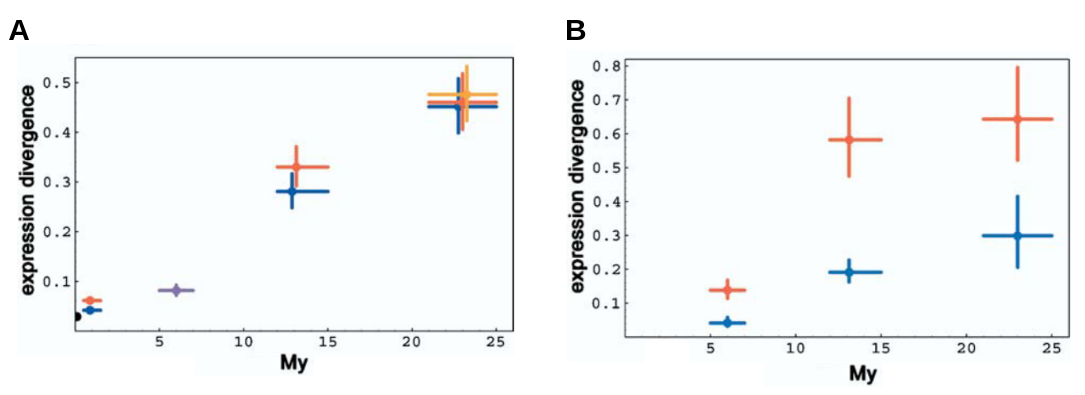
\includegraphics[width=1\textwidth, page=1] {figures/introduction/fig24.png}
 \caption[Divergence des niveaux d'expression des gènes chez les primates.]{
 \textbf{Divergence des niveaux d'expression des gènes chez les primates.}
 \textbf{A.} Différences moyennes d'expression des gènes dans le cerveau au sein et entre primates selon le temps de divergence. Couleurs : rouge, comparaisons entre et avec les humains ; bleu, comparaisons entre et avec les chimpanzés ; violet, comparaisons entre humains et chimpanzés ; orange, comparaisons entre orang-outan et macaque rhésus ; noir, comparaisons entre duplicats expérimentaux. Les barres d'erreur verticales pour l'expression indiquent les intervalles de confiance à 95\% calculés par 10 000 bootstraps. \textbf{B.} Différences moyennes d'expression des gènes dans le cerveau entre humain et primates pour les 25\% des gènes avec l'expression la plus variable (rouge) et la moins variable (bleue) au sein de six humains. Tirée de \citet{khaitovich_neutral_2004}.\\
 }
 \label{fig:Fig24}
\end{figure} 

De la même manière que pour l’évolution des séquences, le rapport entre la divergence entre espèces et la diversité intra-espèce peut permettre de détecter une signature de la sélection positive ou négative \citep{mcdonald_adaptive_1991}. En cas de neutralité stricte, il est attendu que ce rapport soit égal à celui entre le temps de divergence de l'espèce et le temps moyen jusqu'aux ancêtres communs des individus échantillonnés au sein d'une espèce. Autrement dit, il est essentiel de tenir compte de la distance génétique qui sépare les espèces pour évaluer la divergence de l'expression. Dans ces analyses, on fait l'hypothèse que le niveau d'expression observé pour une espèce correspond à un certain optimum adaptatif. Si la variation inter-espèce est supérieure à l’attendu en tenant compte de la variation intra-espèce, alors l’expression du gène semble avoir subi une évolution adaptative vers un nouveau niveau d’expression optimum. A l’inverse si la variance inter-espèce est plus faible qu’attendue selon la distance génétique alors l’expression du gène est probablement sous sélection purifiante ou stabilisante pour conserver le même niveau \citep{khaitovich_neutral_2004}.

\subsection{Evolution de l’expression des gènes}
\label{subsec:evol-expr}

\subsubsection{Comparaison entre espèces proches}
\label{subsec:comp-sp-proche}

Les premières études de l’évolution de l’expression des gènes ont pu être réalisées entre des espèces proches grâce à l’utilisation de sondes génétiques nécessitant une grande proximité de séquence des transcrits \citep{enard_intra-_2002,oleksiak_variation_2002,denver_transcriptional_2005,whitehead_neutral_2006, gilad_expression_2006}. Celles-ci ont confirmé un modèle d’évolution quasi-neutre du niveau d’expression pour la grande majorité des gènes chez des groupes espèces aussi variées que des vers, des primates, des souris ou des poissons. Elles ont montré que les variations intra et inter-population sont positivement corrélées mais que la sélection stabilisante est largement dominante dans l’évolution de l’expression des gènes. Ceci est en accord avec l’idée que la majorité des mutations sont délétères pour l’organisme et sont donc purgées par la sélection naturelle. Pour certains gènes, des changements d’expression plus importants qu'attendus d'après la distance génétique seule ont pu être révélés, signe d’une potentielle évolution adaptative. Par exemple, de nombreux gènes codant pour des facteurs de transcription (\acrshort{FT}s) ont montré un niveau d’expression significativement plus grand dans le foie des individus humains par rapport à d’autres espèces proches de primates \citep{gilad_expression_2006}. Cette observation est particulièrement intéressante car des modifications des niveaux d’expression de ces gènes sont susceptibles de modifier à leur tour l’expression d’autres gènes et ainsi d’affecter plus largement les phénotypes. \\

L’analyse de la variance du niveau d’expression de gènes intra et inter-population a également permis d’identifier des contraintes spécifiques sur certains gènes, reflets de fonctions physiologiques ou écologiques particulières (Figure \ref{fig:Fig25}). Par exemple, en analysant le niveau d’expression des gènes dans plusieurs individus et populations d’un poisson (\textit{Fundulus heteroclitus}), certains gènes ont montré une variance intra-population bien plus importante qu’attendue selon un mode d’évolution neutre \citep{whitehead_neutral_2006}. Ceci est caractéristique d’une sélection balancée, qui permet de maintenir plusieurs optimums du niveau d’expression des gènes au sein d’une population. 

\begin{figure}[h]
 \centering
 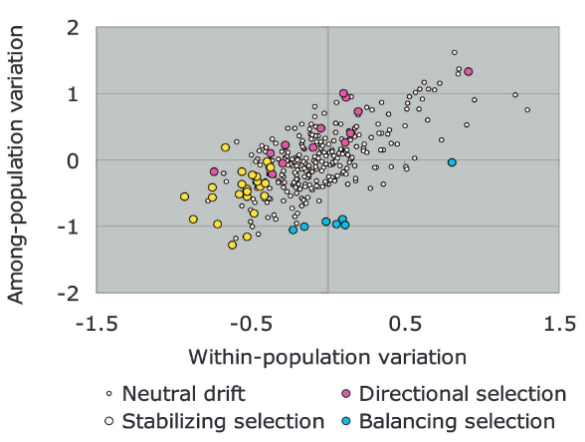
\includegraphics[width=0.7\textwidth, page=1] {figures/introduction/fig25.png}
 \caption[Variation de l'expression des gènes intra et inter-populations, indiquant différents modèles de divergence évolutive.]{
 \textbf{Variation de l'expression des gènes intra et inter-populations, indiquant différents modèles de divergence évolutive.}
 Les logarithmes de la variation de l'expression génique intra- (abscisse) et inter-population (ordonnée) sont représentés. En cas de dérive génétique, la variation intra-population est corrélée à la variation inter-population (cercles vide). D'autres gènes rejettent ce modèle nul. Les gènes soumis à une sélection directionnelle (cercles roses) ont été identifiés comme divergents le long d'un gradient de température de l'habitat après correction de la variance due à la phylogénie, et présentent une variation plus élevée entre les populations qu'au sein de celles-ci. Les gènes les plus influencés par la sélection stabilisante (cercles jaunes) ont une variation plus faible au sein des populations et entre elles que la plupart des gènes, et les gènes soumis à une sélection balancée (cercles bleus) ont une variation plus élevée au sein des populations qu'entre elles. Tirée de \citet{whitehead_neutral_2006}.\\
 }
 \label{fig:Fig25}
\end{figure} 

\subsubsection{Comparaison à plus grande échelle évolutive}
\label{subsec:comp-grande-echelle}

Le développement de techniques de séquençage du \gls{transcriptome} à haut débit a ensuite permis d’analyser l’évolution de l’expression des gènes à plus grande échelle évolutive. La difficulté n’est plus tant de capturer des transcrits suffisamment proches mais de pouvoir identifier correctement les isoformes d’un gène et les relations d’orthologies entre les gènes. La seconde difficulté est de normaliser correctement le niveau d’expression des gènes afin de pouvoir comparer les \glspl{transcriptome} d’espèces distantes (cf \ref{subsec:expression-différentielle}). Ceci est habituellement fait en utilisant les gènes dont l’expression est la moins variable dans la grande majorité des tissus, comme les gènes dits de ménage. 

Brawand et collaborateurs ont analysé l’expression des gènes codants homologues de neuf espèces de mammifères et du poulet \citep{brawand_evolution_2011}. Ils ont montré que la divergence entre espèces des niveaux d’expression pour un même organe reflète la distance génétique (Figure \ref{fig:Fig26}.A). Autrement dit, il est possible de retrouver la phylogénie de ces espèces en comparant les niveaux d’expression des gènes. Ceci confirme les travaux précédents montrant une accumulation des différences linéaires avec le temps de divergence (Figure \ref{fig:Fig24}). Cependant, cette divergence du niveau d’expression se stabilise à grande distance : la différence entre humain et poulet (ayant divergé il y a 300 millions d’années) est similaire à celle entre humain et opossum (160 millions d’années) (Figure \ref{fig:Fig26}.B). Cette observation suggère que la conservation des fonctions essentielles des organes pourrait définir une limite pour la divergence des \glspl{transcriptome}.

\begin{figure}[h]
 \centering
 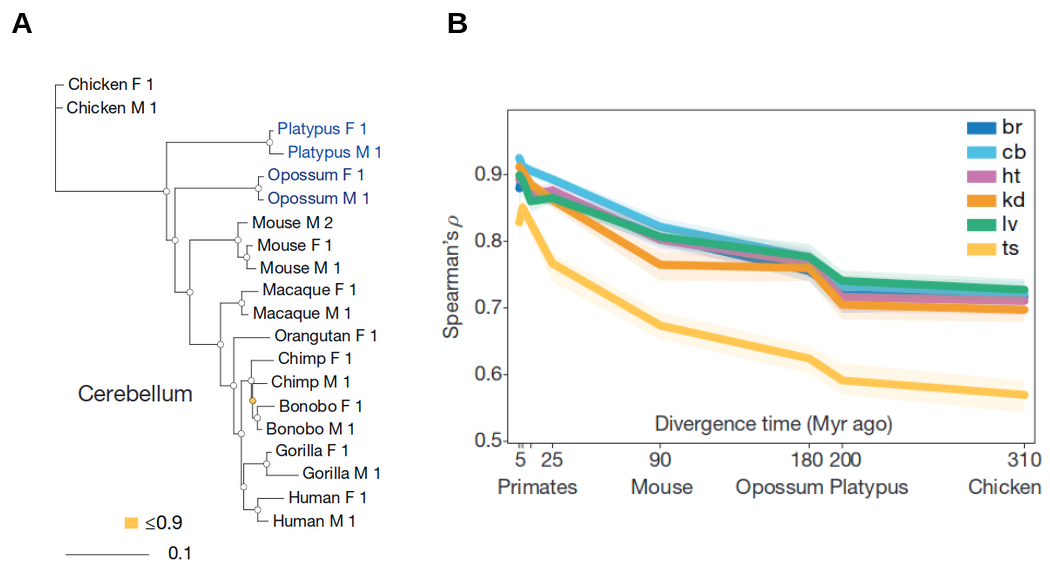
\includegraphics[width=1\textwidth, page=1] {figures/introduction/fig26.png}
 \caption[Corrélation des niveaux d'expression des gènes chez les vertébrés.]{
 \textbf{Corrélation des niveaux d'expression des gènes chez les vertébrés.}
 \textbf{A.} Phylogénie obtenue par Neighbour-Joining à partir de la corrélation de Spearman des niveaux d'expression dans le cervelet de l'ensemble de 5636 gènes orthologues 1-à-1 pour 10 espèces de vertébrés. Les valeurs de bootstrap (1000 tirages aléatoires avec remise) sont indiquées par des cercles blancs ($>$0.9) et jaune ($<$0.9).
 \textbf{B.} Corrélation de Spearman entre le niveau d'expression des gènes chez l'humain et 9 autres espèces selon le temps de divergence entre les espèces. Les enveloppes colorées autour des courbes indiquent les valeurs maximales et minimales de 100 réplicats de bootstraps. Tirée de \citet{brawand_evolution_2011}. \\
 }
 \label{fig:Fig26}
\end{figure} 

Cette étude montre également que les taux d’évolution des niveaux d'expression des gènes diffèrent entre les espèces étudiées. Par exemple, ils sont plus élevés chez les primates que chez les rongeurs. L'évolution plus rapide de l'expression chez les primates s'explique probablement par une sélection moins efficace, plutôt que par des changements adaptatifs plus fréquents. De par un temps de génération plus court, le nombre de mutations par unité de temps est plus élevé chez les rongeurs que chez les primates \citep{li_rates_1996}. On pourrait alors s’attendre à observer une plus grande divergence des niveaux d’expression chez les rongeurs que chez les primates, contrairement à ce qui a été observé. Néanmoins leur importante taille efficace de population permet l’élimination des mutations délétères \citep{ohta_slightly_1973}, contrairement aux primates, qui ont des tailles de population réduites et donc une sélection naturelle moins efficace. Cette observation est également en accord avec une analyse de l'évolution des séquences régulatrices, qui a révélé une évolution accélérée des éléments régulateurs chez les hominidés \citep{keightley_evidence_2005}. L’accumulation de mutations faiblement délétères entraîne une forte divergence des niveaux d’expression dans ces lignées.

\subsubsection{Evolution adaptative et biais potentiels}
\label{subsec:evol-adaptative}

L’étude de l’évolution de l’expression des gènes chez plusieurs espèces de vertébrés permet également de détecter des changements de niveaux d’expression spécifiques aux lignées, dont certains pourraient être le résultat d’une évolution adaptative. Brawand et collaborateurs, ont ainsi modélisé l’évolution de l’expression des gènes le long de la phylogénie selon un modèle neutre et selon un modèle avec un seul optimum du niveau d'expression en prenant en compte la variabilité entre les individus de la même espèce \citep{brawand_evolution_2011}. Un niveau d’expression observé dans une lignée comme étant significativement différent de l’attendu selon ces deux modèles peut alors indiquer un changement d’optimum d’expression. Par exemple, le gène \textit{LIX1} ayant un rôle crucial dans le développement des neurones moteurs a été détecté comme significativement surexprimé dans le cerveau humain. De même, le gène \textit{COL25A1}, lié à plusieurs pathologies neuronales et comportementales, est surexprimé chez les primates dans ce même organe (Figure \ref{fig:Fig27}). 

\begin{figure}[h]
 \centering
 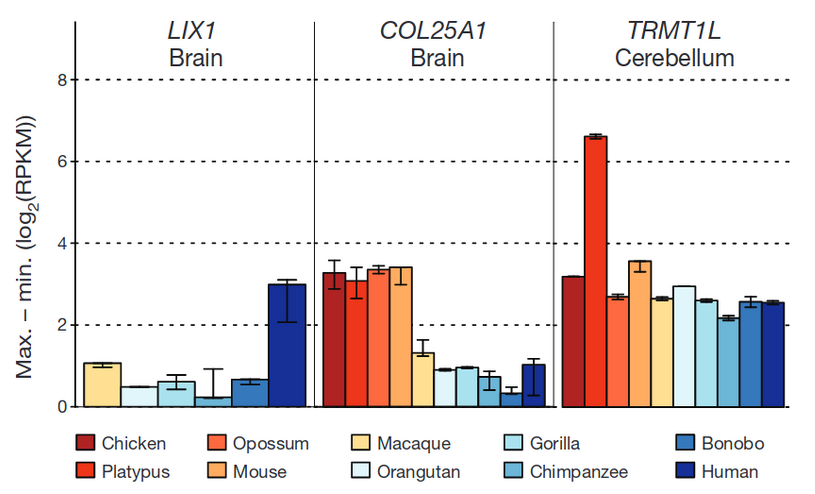
\includegraphics[width=0.8\textwidth, page=1] {figures/introduction/fig27.png}
 \caption[Changement de niveau d'expression spécifique d'une lignée.]{
 \textbf{Changement de niveau d'expression spécifique d'une lignée.}
 Exemple de gènes ayant évolué vers un nouvel optimum du niveau expression dans le cortex préfrontal chez l'humain (\textit{LIX1}), dans le cortex des primates (\textit{COL25A1}) et dans le cervelet de l'ornithorynque (\textit{TRMT1L}). Les barres d'erreurs représente l'étendue des valeurs d'expression au sein des différents individus d'une même espèce et tissu. Tirée de \citet{brawand_evolution_2011}.\\
 }
 \label{fig:Fig27}
\end{figure}

Il est cependant nécessaire de garder à l’esprit que de telles comparaisons sont empreintes de nombreux biais et facteurs confondants, et que les conclusions sur l’attribution de changement du niveau d’expression à la sélection adaptative doivent être prises avec précaution \citep{brawand_evolution_2011}. Outre certains biais techniques précédemment évoqués (cf \ref{subsec:expression-différentielle}) pouvant affecter la mesure des niveaux d’expression, d’autres changements agissant à différentes échelles peuvent affecter les comparaisons. Par exemple, à l’échelle de la séquence, la recombinaison génétique peut entraîner un biais de fixation en faveur des nucléotides G et C, causant une accélération du taux d’évolution \citep{duret_biased_2009}. En agissant sur les éléments \gls{cis}-régulateurs, affectant alors le niveau d’expression des gènes cibles, ce biais peut alors être confondu avec un changement adaptatif \citep{capra_many_2013, duret_comment_2009}. De plus, en estimant le niveau d’expression d’un gène par la quantité de ses transcrits, on omet les nombreuses couches de régulation post-transcriptionnelle qui peuvent permettre de relâcher l’intensité de la sélection purifiante sur la quantité d’\acrshort{ARNm} \citep{wang_transcriptome_2020}. Un changement du niveau d’expression pourrait dans ce cas ne pas avoir d’effet sur le phénotype. Lorsque l'on analyse le \gls{transcriptome} sur des organes complets, il est également probable que des changements de la composition cellulaire spécifique d’une lignée puissent biaiser les comparaisons. L’estimation des niveaux d’expression des gènes à l’échelle cellulaire, notamment par du \acrshort{RNA-seq}” en cellule unique pourraient permettre d’affiner ces comparaisons. Ces exemples de biais potentiels peuvent participer à la mauvaise interprétation de la part adaptative de l’évolution des niveaux d’expression.

\subsection{Variation de l’expression des gènes entre condition}
\label{sub:variation-condition}

Les variations du niveau d’expression des gènes entre espèces peuvent permettre de révéler des changements phénotypiques au sein d’un organe. Cependant les gènes sont généralement exprimés dans plusieurs \glspl{condition} et au sein de différents tissus. Pour comprendre l’évolution de l’expression des gènes, il est nécessaire de comparer les \glspl{transcriptome} au sein de ces différentes \glspl{condition}.

\subsubsection{Comparaison du niveau d’expression entre organes}
\label{subsub:variation-organes}

La comparaison des \glspl{transcriptome} de dix espèces à travers six organes différents a révélé que les différences d’expression des gènes sont bien plus importantes entre les organes qu’entre les espèces (Figure \ref{fig:Fig28}) \citep{brawand_evolution_2011}. Par exemple l’expression des gènes est plus similaire entre le rein de l’humain et le rein du poulet qu’entre le rein et le cerveau d’une même espèce. Cette observation est attendue car la différenciation de ces organes précède la divergence des espèces.\\

\begin{figure}[h]
 \centering
 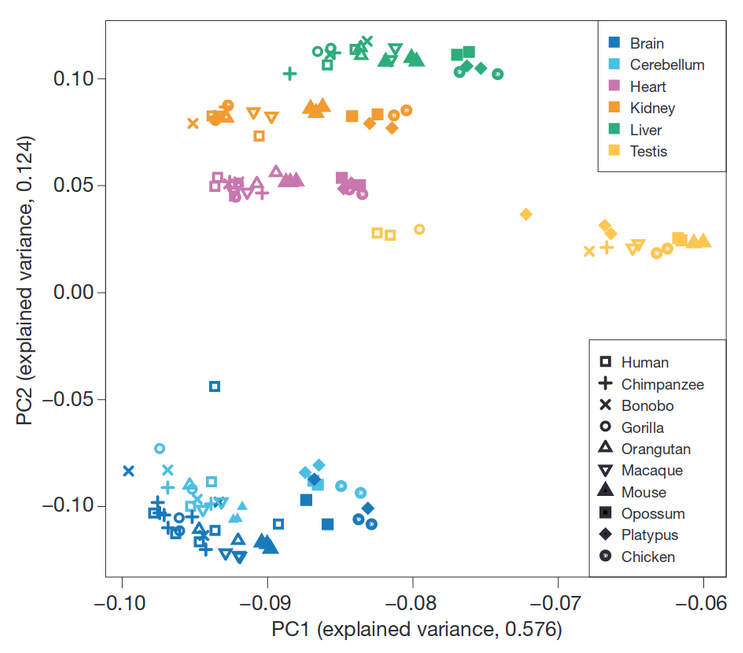
\includegraphics[width=0.8\textwidth, page=1] {figures/introduction/fig28.png}
 \caption[Comparaison des niveaux d'expression entre espèces et organes.]{
 \textbf{Comparaison des niveaux d'expression entre espèces et organes.}
 Analyse des Composantes Principales des niveaux d'expression de 5636 gènes orthologues 1-à-1 de plusieurs individus de 10 espèces de vertébrés au sein de 6 organes différents.
 Tirée de \citet{brawand_evolution_2011}.\\
 }
 \label{fig:Fig28}
\end{figure}

De plus, le taux d’évolution de l’expression des gènes est variable entre les organes. Les testicules par exemple, dont l’évolution phénotypique est connue pour être rapide en raison de pression de sélection sexuelle liée notamment à la compétition spermatique, présentent une évolution très rapide du niveau d’expression \citep{birkhead_postcopulatory_2002}. Ceci peut donc s’expliquer par une sélection adaptative plus forte mais également par une plus faible sélection purificatrice liée à la présence de transcription non-fonctionnelle dans ces organes \citep{soumillon_cellular_2013}. A l’autre extrême, les tissus neuronaux présentent les taux de divergence d’expression les plus faibles. Bien que de nombreux changements phénotypiques aient eu lieu dans ces tissus, notamment l'évolution du cortex préfrontal chez les primates, il semblerait que l’évolution de l’expression des gènes y soit très contrainte. Une plus forte sélection purificatrice sur leur activité pourrait être à l'œuvre. Aussi une plus grande spécialisation des types cellulaires composant les tissus neuronaux pourrait permettre d’affiner avec plus de précision l’activité des gènes et ne serait pas visible à l’échelle de l’organe entier. Un réseau de régulation d’expression plus robuste dans ces tissus pourrait également permettre de conserver une plus grande stabilité en limitant les effets délétères de mutations ponctuelles \citep{khaitovich_evolution_2006}.

\subsubsection{Comparaison des niveaux d’expression des gènes entre stades de développement}
\label{subsub:variation-stade}

Afin de mieux comprendre l’évolution des traits phénotypiques entre les organismes, il est également important d’inclure une dimension temporelle de l’expression des gènes. Les changements de patron d’expression des gènes intervenant aux stades embryonnaires sont susceptibles d’être les plus pertinents d’un point de vue phénotypique. Dans une étude récente, Cardoso-Moreira et collaborateurs ont séquencé les \glspl{transcriptome} de sept espèces de vertébrés dans différents organes à plusieurs stades de développement comparables (Figure \ref{fig:Fig29}) \citep{cardoso-moreira_gene_2019}.

\begin{figure}[h]
 \centering
 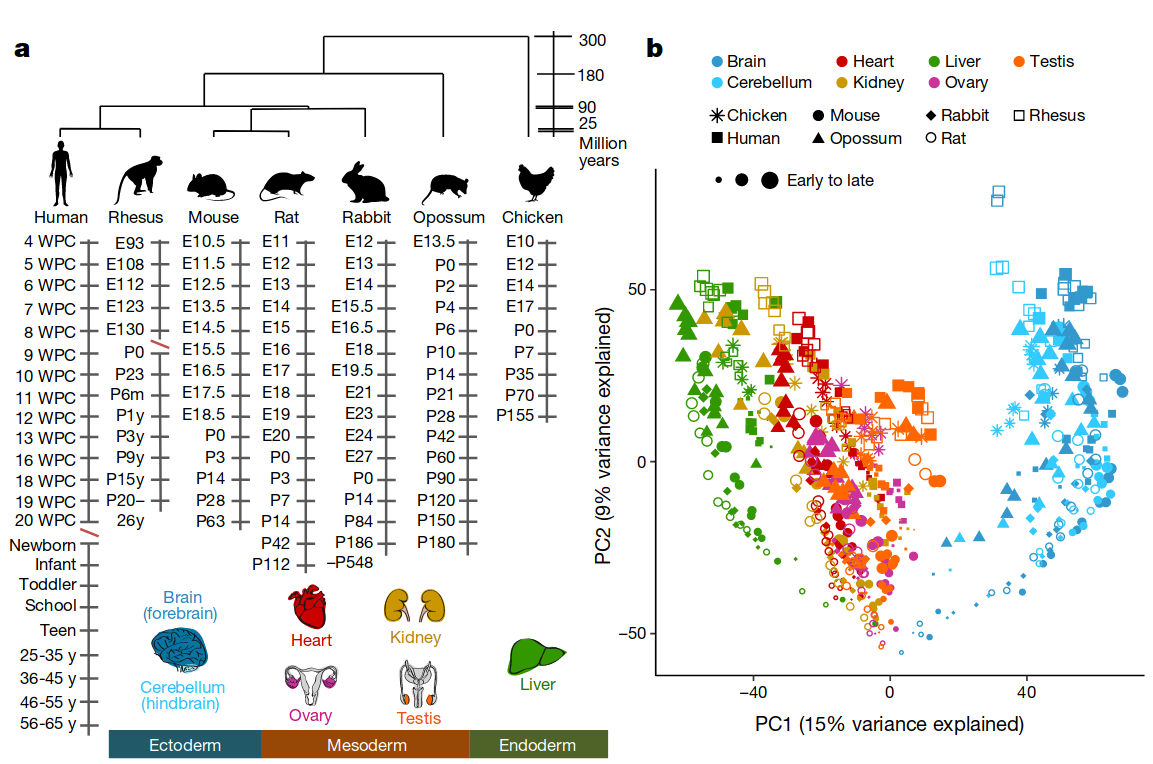
\includegraphics[width=1\textwidth, page=1] {figures/introduction/fig29.png}
 \caption[\glspl{transcriptome} de plusieurs organes à plusieurs stades de développement comparables de plusieurs espèces de vertébrés.]{
 \textbf{\glspl{transcriptome} de plusieurs organes à plusieurs stades de développement comparables de plusieurs espèces de vertébrés.}
 \textbf{A.} Espèces, organes et représentation des stades de développement alignés des échantillons analysés. \textbf{B.} Analyse des Composante Principale basée sur 7 696 gènes orthologues 1-à-1 dans toutes les espèces. Chaque point représente la médiane des réplicats techniques. Tirée de \citet{cardoso-moreira_gene_2019}.\\
 }
 \label{fig:Fig29}
\end{figure}

Comme précédemment, la différence entre les organes étudiés est la plus grande source de variabilité des patrons d’expression des gènes. Cependant, les échantillons prélevés dans des stades précoces sont très similaires entre eux, quelle que soit l’espèce ou l’organe d’origine, avant de diverger de manière progressive au cours du développement. Ceci peut s’expliquer par des modifications du nombre de \glspl{condition} dans lesquelles les gènes sont actifs. Au début du développement, les gènes actifs ont tendance à fonctionner dans de nombreux organes et stades, ce qui contraint leur évolution. Lorsque les organes se différencient et arrivent à maturité, les gènes actifs sont plus spécifiques avec des profils spatio-temporels plus restreints, ce qui peut réduire les contraintes fonctionnelles et faciliter les changements évolutifs. En effet, plus un gène est exprimé dans un grand nombre de tissus et plus son niveau d’expression est conservé \citep{khaitovich_evolution_2006}. Les contraintes évolutives agissant sur le niveau d’expression d’un gène augmentent avec le nombre de \glspl{condition} dans lesquelles le gène est exprimé. Si un gène est exprimé dans l’ensemble des tissus, le caractère délétère d’une mutation affectant son expression dans une seule \gls{condition} suffit pour la contre-sélectionner (Figure \ref{fig:Fig30}).

\begin{figure}[h]
 \centering
 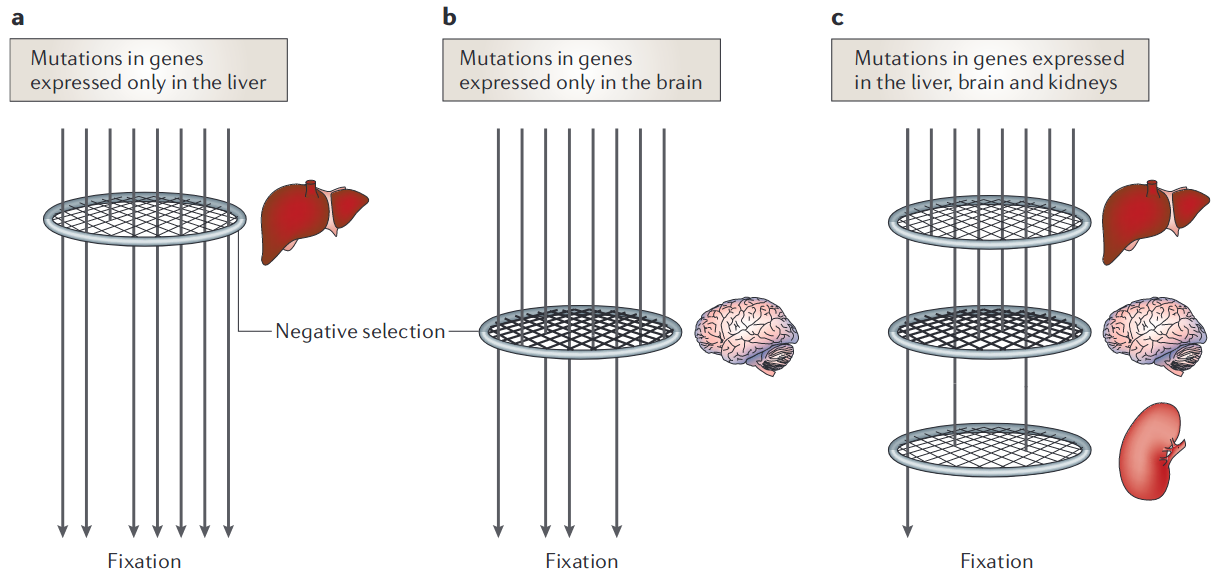
\includegraphics[width=0.9\textwidth, page=1] {figures/introduction/fig30.png}
 \caption[La sélection purifiante sur l'expression des gènes s'accumule avec le nombre de tissus.]{
 \textbf{La sélection purifiante sur l'expression des gènes s'accumule avec le nombre de tissus.}
 Plusieurs mutations affectent le niveau de l'expression des gènes exprimés uniquement dans le foie (\textbf{A}), uniquement dans le cerveau (\textbf{B}) et dans le foie, le cerveau et les reins (\textbf{C}). Les mutations passent ou non le filtre de la sélection purifiante. Les niveaux d'expression des gènes dans le cerveau sont davantage contraints, une plus faible proportion de mutation arrive à fixation. Les contraintes s'additionnent avec le nombre de tissu dans lesquels un gène est exprimé, menant à une plus forte séléction purifiante. Tirée de \citet{khaitovich_evolution_2006}.\\
 }
 \label{fig:Fig30}
\end{figure}

\subsubsection{Evolution des profils d’expression}
\label{subsub:evol-profil}

Avec de telles données il est alors possible de mesurer des profils d’expression entre tissus et/ou au cours du développement, pour chaque gène indépendamment (Figure \ref{fig:Fig31}). Cela permet de comparer l’expression des gènes entre espèces distantes en s’affranchissant des procédures de normalisation visant à homogénéiser les niveaux d’expression des gènes. Les différences observées sont davantage qualitatives que quantitatives et permettent par exemple de déceler des changements majeurs de l’activité d’un gène dans un tissu ou encore des trajectoires temporelles d’expression. Par exemple, on a observé une réduction du niveau d’expression du gène \textit{GRIA3}, important pour de nombreux processus neurophysiologiques, au cours du développement du cerveau humain, alors que pour les autres espèces l’expression de ce gène augmente au cours du développement (Figure \ref{fig:Fig31}) \citep{cardoso-moreira_gene_2019}. Inversement, le gène \textit{MDGA1}, important pour le développement du système nerveux, est exprimé dans les stades précoces et diminue au cours du développement du cerveau chez de nombreuses espèces alors qu’il s’active plus tardivement et augmente avec le temps chez l’humain. Ces changements de trajectoire développementale sont de bons candidats pour expliquer certaines modifications phénotypiques au cours de l’évolution des mammifères.

\begin{figure}[h]
 \centering
 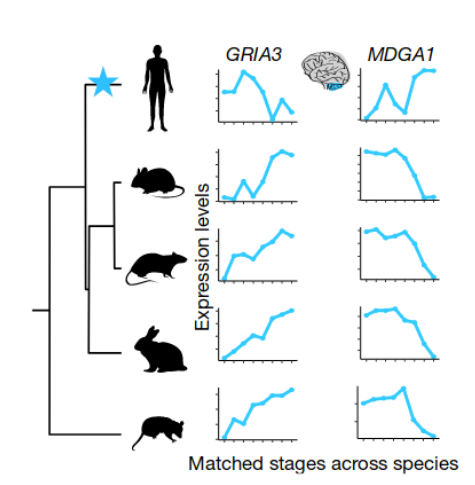
\includegraphics[width=0.6\textwidth, page=1] {figures/introduction/fig31.png}
 \caption[Evolution du profil temporel d'expression d'un gène.]{
 \textbf{Evolution du profil temporel d'expression d'un gène.}
 Exemple des profils temporels d'expression des gènes \textit{GRIA3} (récepteur de glutamate associé à la déficience intellectuel) et \textit{MDGA1} (glycoprotéine importante dans le développement du système nerveux) au cours du développement du cervelet à des stades de développement embryonnaire comparables chez quatre espèces. L'expression de ces gènes a évolué vers une trajectoire différente chez l'humain comparé aux autres espèces. Tirée de \citet{cardoso-moreira_gene_2019}. \\
 }
 \label{fig:Fig31}
\end{figure}

\subsection{\'Evolution de l’expression et de la séquence des gènes}
\label{sub:evol-exp-seq}

La vitesse d’évolution de l’expression des gènes est donc influencée par leur activité dans certains tissus ou stades de développement, ainsi que par leur diversité fonctionnelle, c’est-à-dire leurs rôles dans un grand nombre de contextes. Ces mêmes facteurs influencent également l’évolution des séquences \citep{kuma_functional_1995,hastings_strong_1996}. Il a ainsi été montré que le patron d’expression des gènes est un déterminant majeur des pressions de sélection agissant sur les régions codantes et non codantes des gènes \citep{duret_determinants_2000}. L’évolution de l’expression des gènes et des produits des gènes semblent en effet agir de manière parallèle. Les gènes exprimés dans un plus grand nombre de \glspl{condition} sont également ceux dont les séquences codantes présentent le moins de substitutions non-synonymes, indiquant une sélection purifiante plus importante à l’échelle de la séquence. De même que pour l’expression, les gènes actifs dans le cerveau sont ceux dont la séquence évolue le moins vite, à l’opposé de ceux exprimés dans les testicules (Figure \ref{fig:Fig32}) \citep{khaitovich_parallel_2005}. \\

\begin{figure}[h]
 \centering
 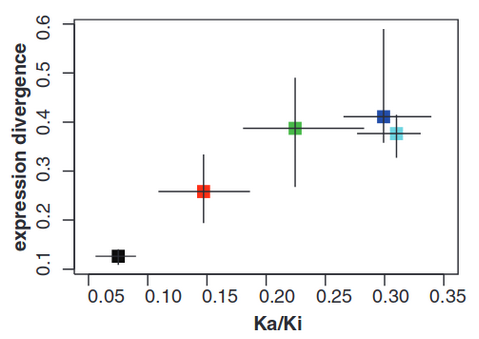
\includegraphics[width=0.6\textwidth, page=1] {figures/introduction/fig32.png}
 \caption[Corrélation entre la divergence d'expression et la divergence des séquences protéiques entre l'humain et le chimpanzé.]{
 \textbf{Corrélation entre la divergence d'expression et la divergence des séquences protéiques entre l'humain et le chimpanzé.} La divergence d'expression est mesurée par la différence médiane entre les niveaux d'expression normalisés des gènes exprimés dans les deux espèces dans le cerveau (noir), le coeur (rouge), les reins (vert), le foie (bleu foncé) et les testicules (bleu clair). La divergence de séquence protéique est mesuré par le nombre de substitutions non-synonyme par site non-synonyme (Ka) normalisé par le nombre de substitution par site dans une fenêtre de 250kb autour du centre du gène (Ki). Les tissus qui présentent une forte divergence de séquence d'acides aminés ont tendance à présenter une forte divergence d'expression (r de Pearson = 0,94, P $<$ 0,05). Les barres d'erreur représentent les intervalles de confiance à 95\% des valeurs médianes calculées à partir de 10 000 réplicats de bootstrap. Tirée de \citet{khaitovich_parallel_2005}.\\
 }
 \label{fig:Fig32}
\end{figure}

De plus, la corrélation positive entre la divergence des séquences codantes et de l’expression des gènes semble constante quelque soit la distance évolutive \citep{warnefors_evolution_2013}. Certaines catégories de gènes semblent néanmoins échapper à cette règle générale. Par exemple, les gènes impliqués dans le développement ou ayant des fonctions neuronales ont tendance à avoir une évolution de l’expression accélérée par rapport à l’évolution de leurs séquences. Les gènes impliqués dans des fonctions immunitaires ou associés à la reproduction mâle ont quant à eux une évolution de leur expression plus rapide de leur séquence codante \citep{haygood_contrasts_2010}.

\section{Evolution de la régulation de l’expression des gènes}
\label{sec:evol-regul}

L’évolution de l’expression des gènes entre espèces et entres \glspl{condition} implique des variations des mécanismes de régulation sous-jacents. Comme nous l’avons vu ces derniers peuvent être nombreux et complexes (cf Partie I \ref{sec:reg-transcription}). L’étude de l’évolution de la régulation de l’expression des gènes peut ainsi se faire à plusieurs niveaux. Je détaillerai ici les bases moléculaires de l’évolution de l’expression agissant au niveau des séquences \gls{cis}-régulatrices \textit{via} des modifications épigénétiques et génétiques.

\subsection{Variations épigénétiques}
\label{subsec:variation-epigenet}

Les variations épigénétiques, comme la modification des histones ou la méthylation de l’ADN affectent la structure de la chromatine et peuvent alors impacter les repliements et/ou l’accessibilité de l’ADN. De telles modifications sont susceptibles d’avoir des conséquences sur la fixation des \acrshort{FT}s ou de l'ARN polymérase sur les éléments régulateurs, modifiant l’expression des gènes concernés. La relation de cause à effet n’est pas évidente car inversement l’activation de la transcription induit également la pose de certaines marques épigénétiques comme H3K27ac sur le promoteur, l’\gls{amplificateur} et le corps du gène pour stabiliser l’ouverture de la chromatine. Les changements épigénétiques peuvent être héritables et pourraient alors expliquer une part importante des variations de l’expression des gènes entre espèces sans affecter la séquence d’ADN en elle-même \citep{lind_evolutionary_2018}. \\

Par exemple, Cain et collaborateurs ont comparé les marques de méthylation d’histone H3K4me3, associées à une augmentation de la transcription, sur des cellules lymphoblastoïdes de plusieurs primates \citep{cain_gene_2011}. Ils ont observé une forte conservation de la position de ces marques mais un enrichissement significatif des différences de H3K4me3 sur les \acrshort{TSS} des gènes différentiellement exprimés. La présence supplémentaire d’une marque H3K4me3 proche d’un gène est associée à une augmentation de son niveau d’expression et inversement lorsque la marque n’est pas observée. Bien que la relation de cause à effet n'ait pas été prouvée, il a été proposé que les variations de H3K4me3 pourraient expliquer jusqu’à 7\% des différences d’expression des gènes entre l’humain et le chimpanzé dans ces cellules \citep{cain_gene_2011}. Une autre étude a confirmé ces résultats et les a complétés avec plusieurs autres marques épigénétiques (H3K4me1, H3K4me3, H3K27ac et H3K27me3) et la présence de l’ARN polymérase II chez plusieurs primates \citep{zhou_epigenetic_2014}. Chacune des marques étudiées est associée à des différences de niveau d’expression des gènes voisins. Prises ensemble elles expliqueraient près de 40\% de la variance des niveaux d’expression des gènes dans les cellules lymphoblastoïdes. En combinant l’analyse de ces marques avec une mesure d’accessibilité de la chromatine (ATAC-seq, cf \ref{subsubsec:ouverture-chroma}), il a également été montré que les variations épigénétiques entre les primates sont associées à l’activité des éléments \gls{cis}-régulateurs \citep{garcia-perez_epigenomic_2021}. Les promoteurs des gènes sont les moins sujets à ces variations alors que les \glspl{amplificateur} actifs présentent des marques épigénétiques les plus divergentes. \\

La méthylation de l’ADN au niveau des cytosines des dinucléotides \acrshort{CpG} est également un facteur important pour l’expression des gènes. Enrichies au niveau de certains promoteurs des gènes, ces dinucléotides peuvent être hyper-méthylés et ainsi modifier les interactions avec d’autres protéines ce qui réduit le niveau d’expression des gènes associés \citep{jones_role_2001}. Cette marque épigénétique peut également être héritable et contribuer à la divergence des niveaux d’expression entre espèces. Entre 11\% à 25\% des gènes différentiellement exprimés entre l’humain et le chimpanzé pourrait être la conséquence de variations de méthylation de l’ADN sur leur promoteur \citep{pai_genome-wide_2011, blake_comparison_2020}. De plus, la divergence de méthylation sur les promoteurs est également associée positivement à la divergence des séquences codantes, ce qui comme précédemment évoqué indiquerait une évolution parallèle entre la régulation et les produits des gènes \citep{hernando-herraez_dynamics_2013}. \\

Cependant ces associations entre modifications épigénétiques et divergence de l’expression ne sont pas nécessairement le reflet de causalité directe et n’excluent pas la part importante des variations au niveau génétique. Des changements des sites de fixation des \acrshort{FT}s pourraient notamment être le déterminant majeur des différences de l’état de la chromatine entre les espèces \citep{mcvicker_identification_2013}.

\subsection{Evolution du répertoire des éléments \textit{cis}-régulateurs}
\label{subsec:evol-repertoire}

Les éléments \gls{cis}-régulateurs dans les génomes peuvent varier en nombre, par des gains ou des pertes, et alors entraîner des variations importantes de l’expression des gènes. L’émergence de nouveaux éléments \gls{cis}-régulateurs peut survenir par l’apparition de nouveaux sites de fixation de facteurs de transcription. Ces éléments pourraient premièrement émerger \textit{de novo} à partir de mutations ponctuelles sur des séquences non-régulatrices. De telles régions régulatrices \textit{de novo} ont été identifiées dans les génomes de poissons téléostéens et semblent être apparues à partir d’anciennes copies dupliquées et dégénérées de gènes codants \citep{eichenlaub_novo_2011}. Cependant, il peut être difficile d’identifier des régions orthologues sur des séquences non-codantes pouvant évoluer rapidement. Il est ainsi délicat de déterminer si ces éléments \gls{cis}-régulateurs sont réellement apparus \textit{de novo} ou à partir d'éléments régulateurs ancestraux ayant divergé suffisamment pour ne plus être identifiables dans d’autres lignées. Les duplications ou transpositions à partir d’éléments \gls{cis}-régulateurs ancestraux semblent également être des mécanismes majeurs dans l’apparition de nouvelles fonctions régulatrices \citep{rebeiz_enhancer_2018}. Chez plusieurs espèces de drosophiles par exemple, 7 \glspl{amplificateur} du gène \textit{shavenbaby} semblent provenir de la duplication à répétition d'une séquence régulatrice ancestrale (Figure \ref{fig:Fig33}) \citep{kittelmann_complex_2021}. Ces différentes copies d’\glspl{amplificateur} ont évolué vers une sous-fonctionnalisation pour activer l’expression de \textit{shavenbaby} de manière spécifique dans différentes cellules de l’embryon de \textit{Drosophila melanogaster}. Ces duplications réduisent la pléiotropie de l’élément \gls{cis}-régulateur unique ancestral et faciliteraient l’évolution de nouveaux patrons d’expression du gène \citep{murugesan_evolution_2022}. \\

\begin{figure}[h]
 \centering
 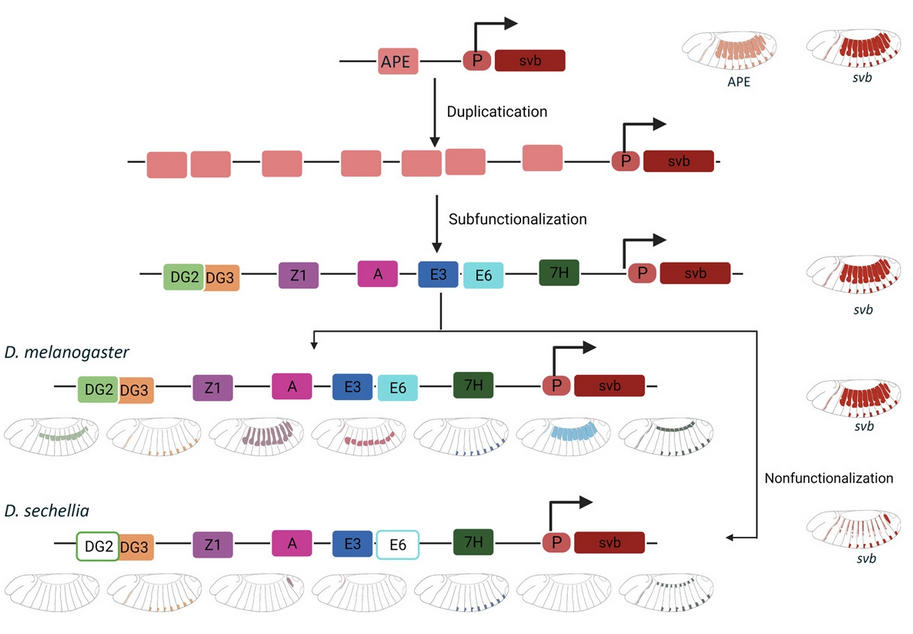
\includegraphics[width=0.9\textwidth, page=1] {figures/introduction/fig33.png}
 \caption[Scénario probable de l'évolution des éléments \gls{cis}-régulateurs du gène \textit{shavenbaby} chez les drosophiles.]{
 \textbf{Scénario probable de l'évolution des éléments \gls{cis}-régulateurs du gène \textit{shavenbaby} chez les drosophiles.}
 Un unique \gls{amplificateur} ancestral pléiotropique (APE) régule l'expression du gène \textit{shavenbaby} (\textit{svb}) dans plusieurs régions de l'embryon chez l'ancêtre commun de plusieurs lignées de drosophiles. APE est dupliqué en sept copies dans les génomes des descendants et évolue vers une sous-fonctionnalisation. Chez \textit{Drosophila melanogaster} chaque copie active l'expression de \textit{svb} dans des régions différentes de l'embryon. Chez \textit{D. sechellia}, certaines copies perdent leur fonction et provoque l'inactivation de \textit{svb} dans certaines régions de l'embryon. Tirée de \citet{murugesan_evolution_2022} à partir de l'étude de \citep{kittelmann_complex_2021}.\\
 }
 \label{fig:Fig33}
\end{figure}

La perte totale ou partielle de la séquence des éléments \gls{cis}-régulateurs peut participer à des changements d’expression des gènes et à l’évolution phénotypique. Chez \textit{Drosophila sechellia}, la perte de la fonction régulatrice de 2 des 7 éléments \gls{cis}-régulateurs de \textit{shavenbaby} élimine ainsi son expression dans certaines cellules et entraîne un changement de la morphologie de la cuticule chez cette espèce (Figure \ref{fig:Fig33}) \citep{kittelmann_complex_2021}. D’autres exemples existent chez les vertébrés, comme la délétion d’un \gls{amplificateur} du gène codant pour le récepteur à l’androgène qui pourrait être à l’origine de la perte des vibrisses (moustache sensorielle) et des épines péniennes chez l’humain \citep{mclean_human-specific_2011}. Chez les cétacés, la réduction des membres inférieurs pourrait être en partie expliquée par plusieurs délétions et substitutions sur un \gls{amplificateur} du gène \textit{TBX4} qui engendreraient une diminution de son expression et ainsi une réduction du développement des membres \citep{liang_divergence_2022}. \\

Il est toutefois important de noter que les délétions peuvent également être à l’origine de gain d'expression ou de gain phénotypique, par exemple en supprimant des éléments \gls{cis}-régulateurs \glspl{inhibiteur} de l’expression des gènes. Inversement, une perte phénotypique peut être la conséquence d’un gain d’activité de gènes qui contrôlent les patrons de développement, tels que la prolifération, la mort ou la migration des cellules. C’est par exemple le cas du gain d’activité du gène \textit{Bmp4}, contrôlant notamment l’apoptose, qui pourrait être lié à la perte du phallus chez le poulet. J'aborderai cet exemple plus en détail dans la Partie \ref{part:chap4}. \citep{herrera_developmental_2013}.

\subsection{Evolution des séquences des éléments \textit{cis}-régulateurs}
\label{subsec:evol-seq-regul}

Plusieurs études ont montré l’importance des mutations des régions régulatrices sur les variations phénotypiques au niveau morphologique, physiologique et comportemental \citep{wray_evolutionary_2007}. Des mutations survenant sur ces séquences peuvent modifier les motifs reconnus par les éléments régulateurs agissant en \gls{trans} comme les \acrshort{FT}s. Schmidt et collaborateurs ont analysé l’occupation de deux \acrshort{FT}s dans le foie de cinq espèces de vertébrés \citep{schmidt_five-vertebrate_2010}. Malgré une reconnaissance de motifs très conservés, les régions de fixation de ces \acrshort{FT}s sont très variables entre espèces. Cette différence de fixation est expliquée par la divergence de séquence des éléments \gls{cis}-régulateurs actifs dans ce tissu. A l’inverse, le facteur de transcription CTCF, qui a un rôle important dans l’organisation tridimensionnelle du génome, possède des sites de fixation très fortement conservés entre espèces de vertébrés \citep{schmidt_waves_2012}. Ceci indique une variabilité importante des pressions de sélection agissant sur les sites de fixation. Entre l’humain et le chimpanzé, qui partagent une forte similarité de séquence, les sites de fixation de l’ARN polymérase II sont largement partagés. Cependant près de 32\% d’entre eux montrent une différence quantitative de la présence de l’ARN polymérase sur leurs séquences \citep{kasowski_variation_2010}. Cette différence est expliquée par des mutations d’un seul nucléotide (SNP) ou des variations structurelles comme des inversions qui pourraient modifier l’affinité de l’ARN polymérase II avec ces sites. De plus, les changements de fixation de cette polymérase sont corrélés avec les divergences des niveaux d’expression de plusieurs gènes entre l’humain et le chimpanzé.

\subsubsection{Evolution des séquences promotrices}
\label{subsubsec:evol-seq-promo}

Au niveau des séquences des promoteurs, le taux d’évolution semble être très variable entre gènes mais aussi entre les espèces \citep{taylor_heterotachy_2006}. En tenant compte des variations locales des taux d'évolution neutre pour éviter les biais de fixation, des études montrent que la divergence de certains promoteurs pourrait être le fruit d’une évolution adaptative chez l’humain \citep{haygood_promoter_2007, torgerson_evolutionary_2009}. Notamment, l’évolution de ces séquences promotrices pourrait être responsable de changement d’expression de gènes impliqués dans des processus du développement du cerveau et du système nerveux. Dans des espèces où la sélection purifiante est plus efficace comme chez les souris, l’évolution des séquences \gls{cis}-régulatrices pourrait également être associée à une plus grande part de sélection positive et adaptative que celle des séquences codantes \citep{halligan_contributions_2013}.

\subsubsection{Evolution des séquences des amplificateur}
\label{subsubsec:evol-seq-enh}

Une comparaison des profils de fixation des facteurs de transcription entre la souris et l’humain a montré que les sites de fixation présents sur les promoteurs sont davantage conservés que ceux présents sur les \glspl{amplificateur} distaux \citep{cheng_principles_2014}. La majorité des éléments \gls{cis}-régulateurs, particulièrement les \glspl{amplificateur} semblent subir une évolution très rapide de leur séquence chez les mammifères \citep{villar_enhancer_2015}. Il existe cependant des variations dans le taux d’évolution. Certains sont très conservés et régulent des processus fondamentaux tissu-spécifiques \citep{ballester_multi-species_2014} ou sont actifs dans de nombreux tissus \citep{cheng_principles_2014}. D’autres sont beaucoup plus variables et pourraient être associés à des gènes sous sélection positive. \\

Par exemple, la séquence et l’activité de l’\gls{amplificateur} \acrshort{ZRS} sont très fortement conservées à l’échelle des vertébrés \citep{kvon_progressive_2016}. Ceci s’explique par une forte pression purifiante car comme nous l’avons vu précédemment les effets de certaines mutations sur \acrshort{ZRS} sont très fortement délétères sur l’expression de \acrshort{SHH} et le développement des membres. Cependant chez les serpents, des tétrapodes qui ont perdu leurs membres, cet \gls{amplificateur} a subi une accumulation de mutations dont d’importantes délétions. Le remplacement par transgénèse du \acrshort{ZRS} de la souris par la séquence homologue du python entraîne une réduction importante des membres, signe de la perte de sa fonction régulatrice sur \acrshort{SHH} (Figure \ref{fig:Fig34}). La régénération artificielle d’un seul site de fixation des facteurs de transcription ETS, très conservé chez les vertébrés, sur la séquence de \acrshort{ZRS} du python résulte en un regain d’activité de \acrshort{SHH} et permet le développement normal des membres chez la souris (Figure \ref{fig:Fig34}.B) \citep{lettice_opposing_2012}. Cette variation de quelques nucléotides souligne l’importance de l’évolution des \glspl{amplificateur} pour la divergence phénotypique. 

\begin{figure}[h]
 \centering
 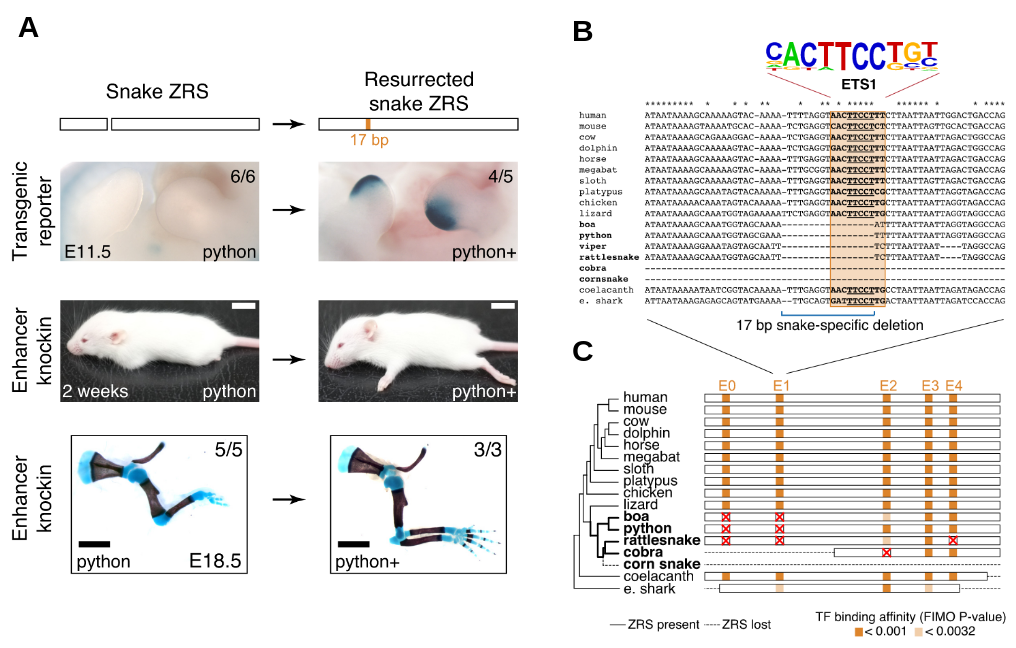
\includegraphics[width=1\textwidth, page=1] {figures/introduction/fig34.png}
 \caption[Résurrection \textit{in vivo} de la fonction de l'\gls{amplificateur} \acrshort{ZRS} du python.]{
 \textbf{Résurrection \textit{in vivo} de la fonction de l'\gls{amplificateur} \acrshort{ZRS} du python.}
 \textbf{A.} A gauche : transgénèse de l'\gls{amplificateur} \acrshort{ZRS} du python dans une souris. A droite : transgénèse de l'\gls{amplificateur} \acrshort{ZRS} du python édité pour inclure 17 paires de base très conservées chez les vertébrés dans une souris. De haut en bas : Activité \textit{in vivo} du \acrshort{ZRS} intégré dans les bourgeons des membres d'une souris au stade embryonnaire E11.5. Le gène rapporteur \textit{LacZ} permet de colorer les cellules lorsque \acrshort{ZRS} est actif. Phénotype de la souris au bout de 2 semaines. Radio du membre de la souris au stade embryonnaire E18.5. 
 \textbf{B.} Alignement d'une partie de la séquence de \acrshort{ZRS} de plusieurs vertébrés. Les 17 paires de bases perdues chez les serpents contiennent un motif reconnu par le facteur de transcription ETS1. 
 \textbf{C.} Distribution des sites de fixation de ETS1 sur la séquence de \acrshort{ZRS} chez les vertébrés. Les croix rouges indiquent la perte du motif. Tirée de \citet{kvon_progressive_2016}. \\
 }
 \label{fig:Fig34}
\end{figure}

De plus, la modification de la séquence des éléments \gls{cis}-régulateurs peuvent participer à l’émergence de nouvelle fonction. Chez plusieurs espèces de drosophiles, l’expression convergente du gène \textit{yellow}, notamment responsable du patron de coloration, est par exemple fortement dépendante de quelques éléments \gls{cis}-régulateurs \citep{prudhomme_repeated_2006}. Chez deux espèces, plusieurs substitutions sur deux éléments \gls{cis}-régulateurs entraînent un gain d’expression du gène dans plusieurs tissus et une coloration convergente. Inversement, la perte convergente de cette coloration chez deux autres espèces serait liée à des mutations faisant perdre l'activité d’un même \gls{amplificateur} de \textit{yellow}. Le gain de fonction régulatrice à partir de l’évolution d’éléments \gls{cis}-régulateurs ancestraux est ainsi probablement un mécanisme important dans l’adaptation morphologique des espèces \citep{koshikawa_enhancer_2015}.

\subsection{Activité des éléments \textit{cis}-régulateurs}
\label{subsec:evol-seq-enh}

L’activité des éléments \gls{cis}-régulateurs, c’est-à-dire leur capacité à réguler l’expression de gènes, au sein des différentes \glspl{condition} cellulaires est également un facteur important à prendre en considération. Leur patron d’activité peut en effet être modifié et alors impacter l’expression des gènes cibles indépendamment de la divergence de leur séquence. Des modifications épigénétiques, comme l’accessibilité de la chromatine ou les modifications d’histones, peuvent ainsi être à l’origine de gains d’activité d’éléments \gls{cis}-régulateurs existants, ce qui impacte l’expression des gènes cibles dans de nouveaux tissus ou contextes cellulaires \citep{rebeiz_evolutionary_2011, xin_enhancer_2020}. \\

L’activité de la majorité des éléments \gls{cis}-régulateurs évolue très rapidement chez les mammifères \citep{xiao_comparative_2012, cotney_evolution_2013, villar_enhancer_2015}. L’activité mesurée par la présence de marques épigénétiques H3K27ac (\gls{amplificateur} actif) et H3K4me3 (promoteur actif) dans le foie de vingt espèces montre ainsi que plus de la moitié des \glspl{amplificateur} dont les séquences sont alignables sont actifs dans une seule espèce \citep{villar_enhancer_2015}. Ceci représente environ 10 000 éléments uniques à chacune des espèces étudiées. L’activité des promoteurs quant à eux est majoritairement conservée chez ces espèces, en accord avec l’évolution plus lente de leur séquence évoquée précédemment \citep{cheng_principles_2014}. Les \glspl{amplificateur} espèce-spécifiques semblent avoir évolué au sein de chaque lignée majoritairement à partir de séquences d’ADN ancestrales non-codantes déjà présentes \citep{villar_enhancer_2015}. Le gain d’activité par des modifications épigénétiques pourrait également permettre de moduler différemment les niveaux d’expression. En effet de tels gains d’activité des \glspl{amplificateur} sont associés avec l’augmentation des niveaux d’expression dans le développement des membres de l’humain par rapport au macaque \citep{cotney_evolution_2013}. \\

Comme nous l’avons vu pour \acrshort{SHH} et \acrshort{ZRS}, un élément \gls{cis}-régulateur crucial d’un gène peut se localiser dans l’intron d’un autre gène. Cette structure peut fortement contraindre la localisation des deux gènes pour se maintenir en synténie, c'est-à-dire en proximité sur la séquence. Dans une étude récente, Wong et collaborateurs ont analysé des paires de gènes voisins dont la synténie est fortement conservée à l’échelle des métazoaires \citep{wong_deep_2020}. Ils ont ainsi pu associer certains \glspl{amplificateur} présents dans ces régions en micro-synténie dans le génome de l’éponge (\textit{Amphimedon queenslandica}) à des \glspl{amplificateur} situés dans des régions orthologues chez des vertébrés. Les séquences de ces \glspl{amplificateur} sont fortement divergentes mais ceux-ci présentent une forte conservation d’activité mesurée par la marque H3K4me1. La transgénèse d’un de ces \glspl{amplificateur} de l’éponge avec un gène indicateur de son activité (Green Fluorescent Protein ou \acrshort{GFP}) dans le génome du poisson-zèbre a montré un patron d’activité cellule-spécifique similaire à celui de l’\gls{amplificateur} du poisson-zèbre de la région micro-synténique orthologue. Ceci indique que les \acrshort{FT}s du poisson-zèbre reconnaissent des sites de fixation sur cet \gls{amplificateur}. En analysant le nombre et la diversité des \acrshort{FT}s se fixant sur les \glspl{amplificateur} de l’éponge dans des régions micro-synténiques, cette étude a permis de proposer des \glspl{amplificateur} orthologues chez le poisson-zèbre, la souris et l’humain conduisant à des patrons d’activité similaires. Ainsi certains éléments \gls{cis}-régulateurs pourraient subir une forte divergence de séquence mais conserver leur fonctionnalité en fixant une configuration similaire de \acrshort{FT}.

\subsection{Réarrangements génomiques}
\label{subsec:rearrangement}

La présence d’interactions régulatrices à longue distance entre les promoteurs des gènes et les éléments \gls{cis}-régulateurs suggère que les réarrangements génomiques peuvent avoir un rôle important dans l’évolution de l’expression des gènes. Ces mutations à grande échelle, telles que les délétions, duplications, inversions et translocations de segments chromosomiques, impliquent une réorganisation importante des génomes. Grâce à des approches comparatives ou par des expériences de manipulation génétique, il est possible d’étudier l’effet des réarrangements sur l’évolution de l’expression des gènes. C’est notamment par le biais de délétions et d’inversions induites sur des embryons de souris que les premières études ont permis de décrire la structure des paysages régulateurs des gènes du développement \citep{tschopp_genetic_2011}. \\

Des réarrangements qui perturbent le contact entre le promoteur de \acrshort{SHH} et son \gls{amplificateur} \acrshort{ZRS} provoquent des changements importants de l’expression du gène et ont des conséquences sur le développement des membres (Figure \ref{fig:Fig35}) \citep{symmons_SHH_2016}. En faisant varier la distance entre ces deux régions grâce à des séries de délétions et inversions dans des génomes de souris, cette étude a cherché à caractériser les limites de l’action de \acrshort{ZRS} sur \acrshort{SHH}. Dans la mesure où les deux loci restent à l’intérieur d’un certain domaine (ou \acrshort{TAD}, cf \ref{subsubsec:TAD-boucle}), la distance qui les sépare sur le génome linéaire n’a pas d’influence significative sur l’expression du gène. Cependant, en dehors de ce domaine, plus la distance qui sépare \acrshort{ZRS} du promoteur de \acrshort{SHH} est grande et moins le gène est exprimé. Ceci peut s’expliquer par une diminution de la probabilité de contact entre les deux régions. La rupture de la relation régulatrice résulte alors en un développement anormal des membres. Cette étude démontre également que l’organisation spatiale de l’ADN peut permettre de relâcher une partie de la contrainte de proximité sur le génome entre deux régions devant être physiquement proches pour fonctionner. Tant que le repliement de la chromatine permet une proximité ou “synténie spatiale”, une certaine variabilité de distance sur le génome serait permise entre un gène et ses éléments \gls{cis}-régulateurs. Des régions distantes dans le génome humain mais proches dans celui de la souris ont ainsi une plus grande probabilité d’être en contact dans les cellules humaines qu’attendu par hasard \citep{veron_close_2011}.

\begin{figure}[h]
 \centering
 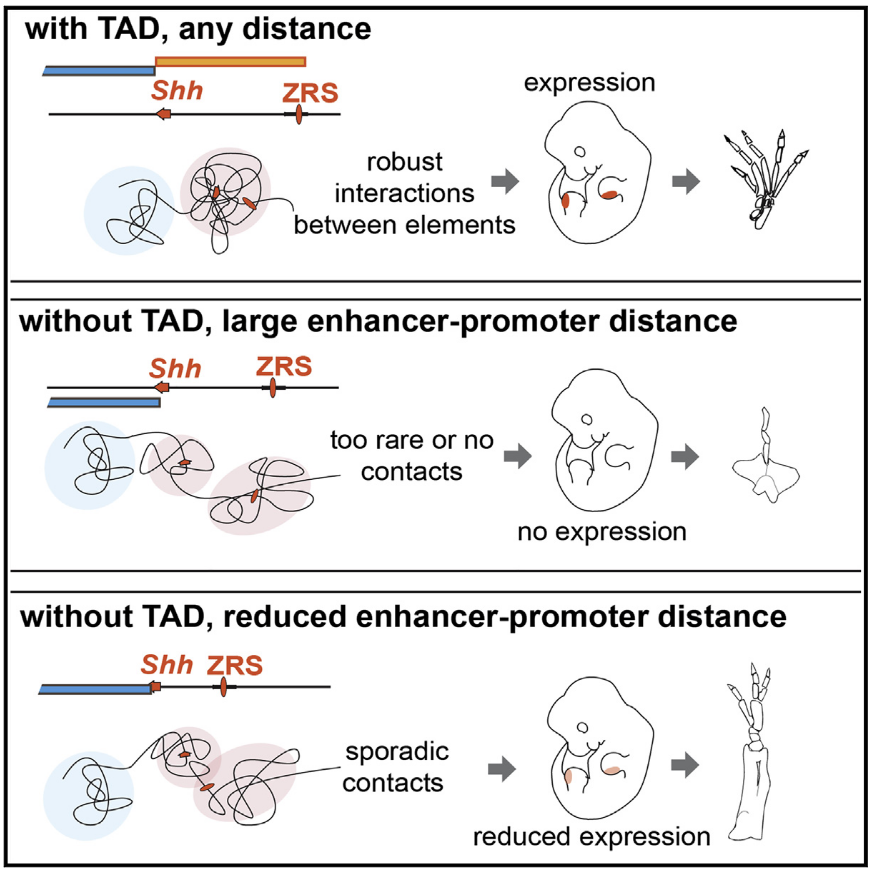
\includegraphics[width=0.7\textwidth, page=1] {figures/introduction/fig35.png}
 \caption[Schéma bilan des conséquences de réarrangements génomiques entre \textit{Shh} et ZRS.]{
 \textbf{Schéma bilan des conséquences de réarrangements génomiques entre \textit{Shh}et ZRS.}
 Des délétions et inversions sont induites entre les deux loci dans les génomes d'embryons de souris. \textbf{En haut}, \textit{Shh}et ZRS restent localisés dans le même domaine d'association topologique (TAD). Quelque soit la distance génomique qui les sépare, les deux régions sont en proximité physique dans le noyau, l'expression de \textit{Shh}dans le bourgeon des membres est inchangée et la formation des membres est normale. \textbf{Au milieu}, \textit{Shh}et ZRS sont séparés par une grande distance génomique et ne sont plus localisés dans le même TAD. Les contacts de chromatine entre les régions sont rares, \textit{Shh}n'est pas exprimé dans le bourgeon des membres et les membres sont tronqués. \textbf{En bas}, \textit{Shh}et ZRS sont séparés par une faible distance génomique mais ne sont pas dans le même TAD. Des contacts sporadiques de la chromatine sont observés entre les loci, \textit{Shh}est exprimé à un faible niveau, les membres se développent avec des malformations. 
 Tiré de \citet{symmons_SHH_2016}. \\
 }
 \label{fig:Fig35}
\end{figure}

Un réarrangement peut également engendrer l’adoption d’un élément \gls{cis}-régulateur par un gène, comme cela semblerait être le cas pour une malformation des membres chez l’humain \citep{lettice_enhancer-adoption_2011}. Chez un individu atteint de cette maladie, suite à une inversion d’une région de plus de 500kb, le gène \acrshort{SHH} est relocalisé. En imitant cette inversion dans le génome de la souris, le gène \acrshort{SHH} est exprimé de façon anormale dans le cerveau et dans les membres et ne semble plus sous le contrôle de \acrshort{ZRS}. Cependant, \acrshort{SHH} est tout de même actif dans le bourgeonnement des membres. Il présente un patron d’expression similaire aux gènes normalement contrôlés par un autre élément \gls{cis}-régulateur fortement conservé et actif dans les membres nommé HCNE2. Bien que la présence d’un contact n'ait pas été testé, le rapprochement de \acrshort{ZRS} à 190kb de HCNE2 suite à cette inversion semble expliquer l’expression anormale du gène dans ce tissu. \\

En comparant conjointement l’organisation des génomes et l’expression des gènes dans le cerveau de l’humain et du chimpanzé, Marquès-Bonet et collaborateurs ont montré que le nombre de réarrangements sur un chromosome est associé à l’augmentation des différences d’expression des gènes de ce chromosome \citep{marques-bonet_chromosomal_2004}. Néanmoins les gènes proches des points de cassure ne présentent pas nécessairement des différences d’expression \citep{munoz_detection_2012}. Les réarrangements observables étant ceux ayant passé le filtre de la sélection naturelle, la majorité d’entre eux n’affectent probablement pas le fonctionnement des gènes. Certains de ces réarrangements pourraient cependant avoir des rôles adaptatifs importants. Il a par exemple été observé que les points de cassure entre l’humain et le macaque sont enrichis dans des régions riches en gènes associés à des processus immunitaires \citep{ullastres_unraveling_2014}. Ces réarrangements auraient pu faciliter des changements de régulation de ces gènes et participer à des adaptations spécifiques. \\

Le paysage \gls{cis}-régulateur pourrait donc induire des contraintes sur la fréquence et la localisation des réarrangements et être ainsi une force majeure de l’évolution de l’organisation des génomes \citep{mongin_long-range_2009}. Ceci expliquerait notamment que de larges régions du génome puissent être restées intactes au cours de l’évolution des vertébrés alors que d’autres sont enrichies en cassures génomiques \citep{naville_long-range_2015, berthelot_3d_2015}. Il a notamment été proposé que la conservation évolutive de la proximité entre des gènes et des séquences \gls{cis}-régulatrices puisse être un indicateur de leur association fonctionnelle \citep{ahituv_mapping_2005,mongin_long-range_2009, clement_enhancergene_2020}. Cette conservation de proximité est corrélée à la présence de marques épigénétiques caractéristiques d’éléments \gls{cis}-régulateurs et pourrait également servir de prédicteur de leur activité \citep{naville_long-range_2015}. 

\section{Relation entre l’évolution de l’expression des gènes et l’évolution du paysage \textit{cis}-régulateur}
\label{sec:relation-paysage-exp}

Peu d’études se sont attachées à étudier simultanément l’évolution de l’expression des gènes et l’évolution du paysage \gls{cis}-régulateur à l’échelle de l’ensemble du génome. D’un côté, les paysages \gls{cis}-régulateurs de l’expression des gènes évoluent rapidement à la fois au niveau des séquences et au niveau de l’activité des \glspl{amplificateur} \citep{cheng_principles_2014, villar_enhancer_2015}. A l'inverse, les patrons d’expression des gènes sont relativement bien conservés entre espèces lorsque l’on compare des tissus similaires \citep{brawand_evolution_2011, necsulea_evolutionary_2014, cardoso-moreira_gene_2019}. Ce paradoxe pourrait d’abord être expliqué par la redondance fonctionnelle des paysages \gls{cis}-régulateurs. Comme précédemment mentionné, le paysage \gls{cis}-régulateur d’un gène peut comporter de nombreux éléments \gls{cis}-régulateurs qui peuvent être redondants (cf \ref{subsec:complexite}). Les gènes associés à de nombreux éléments \gls{cis}-régulateurs semblent avoir une expression plus stable au cours de l’évolution \citep{berthelot_complexity_2018}. La redondance fonctionnelle pourrait réduire les pressions évolutives sur chaque élément \gls{cis}-régulateur \citep{frankel_phenotypic_2010,osterwalder_enhancer_2018, kvon_enhancer_2021}. Une mutation ponctuelle sur un élément redondant aurait un impact moins important sur la valeur sélective de l’individu et serait donc moins soumise à la sélection purifiante si le gène cible possède un paysage de régulation complexe. Potentiellement, plus une séquence serait redondante fonctionnellement et plus elle pourrait évoluer de façon neutre sans impacter l’expression des gènes cibles. L’émergence de nombreux éléments \gls{cis}-régulateurs spécifiques de chaque lignée de mammifères indiquerait un renouvellement rapide au sein de paysages \gls{cis}-régulateur permissifs et modulables \citep{villar_enhancer_2015}. De plus, les éléments \gls{cis}-régulateurs pourraient avoir une contribution variable à l’expression des gènes cibles. Par exemple, les \glspl{amplificateur} ayant récemment émergé sont ceux qui contribuent le moins à la robustesse et au niveau d’expression des gènes \citep{berthelot_complexity_2018}. Les éléments évoluant rapidement pourraient alors n’avoir que peu d’impact sur l’expression des gènes.\\

Une autre possible explication à cette différence pourrait être plus technique et résider dans une mauvaise attribution des éléments \gls{cis}-régulateurs à leurs gènes cibles. La majorité des études réalisées jusqu’à maintenant ont défini le paysage \gls{cis}-régulateur d’un gène par une approche de voisinage. Dans cette approche les éléments \gls{cis}-régulateurs sont associés au gène voisin le plus proche, jusqu’à une certaine distance génétique ou jusqu’au gène suivant. Cette définition est pertinente car elle permet d’inférer un grand nombre de relations régulatrices qui semblent avoir un sens biologique \citep{kundaje_integrative_2015}, et surtout ne nécessite pas d’effectuer des expérimentations particulières. Cependant nous avons vu précédemment que l’accès à la conformation tridimensionnelle du génome a permis d’observer des boucles de chromatine qui peuvent induire des relations régulatrices plus complexes. L’exemple du gène \acrshort{SHH} et de \acrshort{ZRS} illustre parfaitement qu’un élément \gls{cis}-régulateur peut agir à grande distance sur ses cibles sans impacter l’expression des gènes voisins. Le manque de relation évidente entre la divergence du paysage \gls{cis}-régulateur et la divergence de l’expression des gènes pourrait alors s’expliquer en partie par l’attribution incomplète (ou même partiellement erronée) d’éléments \gls{cis}-régulateurs aux gènes cibles. De plus, certains éléments \gls{cis}-régulateurs prédits pourraient être fonctionnels, c’est-à-dire reconnus par des facteurs de transcription et/ou ayant des marques épigénétiques caractéristiques, sans être associés à aucun gène par les diverses méthodes computationnelles. Plus généralement, les imprécisions de la construction des paysages \gls{cis}-régulateurs à grande échelle pourraient cacher les subtilités de la régulation de l’expression des gènes. \\

    \chapter{Objectifs de cette thèse}
\label{chap:objectifs}

Au cours de cette thèse, je me suis d’abord intéressé à définir les paysages \gls{cis}-régulateurs de l’expression des gènes chez l’humain et la souris à partir des contacts de la chromatine et de prédictions d’éléments \gls{cis}-régulateurs. Dans le Chapitre 2, mon objectif a été de comparer ces paysages \gls{cis}-régulateurs avec ceux obtenus par les méthodes les plus généralement employées qui consistent à associer les gènes aux éléments \gls{cis}-régulateurs voisins. Je me suis ensuite attaché à savoir si les contacts de chromatine pouvaient permettre d’attribuer des fonctions différentes aux éléments \gls{cis}-régulateurs.\\

Dans le Chapitre 3, je me suis demandé comment les paysages \gls{cis}-régulateurs tels que mesurés par les contacts de chromatine évoluent chez plusieurs espèces de vertébrés. Particulièrement, j’ai cherché à étudier si les paysages \gls{cis}-régulateurs imposent des contraintes sur l’évolution de l’organisation des génomes. J’ai également analysé les associations entre la structure des paysages \gls{cis}-régulateurs et l’expression des gènes en termes de niveaux et d’étendue de l’expression au sein de plusieurs tissus et stades embryonnaires chez l’humain et la souris. J’ai ensuite investigué les relations entre l’évolution des profils d’expression des gènes et l’évolution des paysages \gls{cis}-régulateurs mesurés par la divergence des séquences, de synténie entre gène et éléments \gls{cis}-régulateur et des contacts de chromatine.\\

Finalement dans le Chapitre 4, j’ai cherché à comprendre comment l’évolution du paysage \gls{cis}-régulateur peut impacter l’évolution d’un trait phénotypique. Je me suis pour cela attaché à comprendre la relation entre l’évolution des éléments \gls{cis}-régulateurs et la perte convergente du phallus chez les oiseaux. Grâce aux profils d’expression des gènes chez le poulet et le canard ainsi qu’à une étude comparative des génomes de plusieurs oiseaux, j’ai cherché à détecter des séquences \gls{cis}-régulatrices qui pourraient expliquer ce changement phénotypique majeurs survenant lors du développement. Pour cette étude, le génome d’un oiseau nouvellement séquencé a été utilisé, j’ai donc assemblé son génome et analysé ses caractéristiques.

    \part{Associer les gènes aux éléments cis-régulateurs}
    \label{part:chap2}
    \newpage
Un des défis majeurs pour comprendre la régulation de l’expression d’un gène reste encore aujourd’hui de définir quels sont les facteurs qui agissent sur sa transcription. Comme précédemment décrit, les mécanismes de régulation de la transcription des gènes sont nombreux et peuvent agir en cis, sur la même molécule d’ADN, ou en trans par le biais de molécules en circulation dans le noyau (cf Chapitre 1 \ref{chap:regulation-de-expression}). Bien que leur nombre ne soit pas précisément connu, il existe vraisemblablement des centaines de milliers d’éléments \gls{cis}-regulateurs, dépassant très largement le nombre de gènes \citep{encode_project_consortium_integrated_2012}. De nombreuses méthodes permettent de détecter ou prédire la localisation et l’activité des éléments \gls{cis}-régulateurs (cf Chapitre 1 \ref{sec:identif-cis}). Cependant il est encore difficile de définir les gènes cibles de chaque élément \gls{cis}-régulateur. Le rapprochement physique par une boucle de la chromatine est le modèle le plus généralement admis pour expliquer l’activation de l’expression des gènes par les amplificateurs \citep{blackwood_going_1998,bulger_looping_1999, marsman_long_2012}. De nombreux facteurs agissent pour établir de tels repliements, afin de permettre aux amplificateurs de recruter la machinerie de transcription au niveau des promoteurs. La mise en place sélective des paires de promoteur et d’élément \gls{cis}-régulateur pourrait s’effectuer grâce à des modifications précises de la chromatine (ouverture, modifications d’histones, fixation de protéines,...) et par l’action combinée de facteurs agissant en trans se fixant sur les séquences des deux éléments de façon spécifique \citep{ernst_interplay_2013}. La détection et la validation expérimentale de telles paires régulatrices peuvent s’avérer complexes et coûteuses. En effet, observer l’effet d’un éléments \gls{cis}-régulateur sur un gène peut être délicat en raison de la spécificité de la relation (régulation restreinte à un type cellulaire, stade de développement, dépendante de facteurs environnementaux…) ou de nombreux facteurs confondants (redondance fonctionnelle, mécanismes de compensation…). Plusieurs approches d’inférence computationnelle ou expérimentale tentent de prédire les associations entre gènes et éléments \gls{cis}-régulateurs.\\

Au cours de ce chapitre je vais d’abord décrire certaines approches couramment utilisées pour associer les gènes aux élements \gls{cis}-régulateurs. Je m’attacherai ensuite à détailler comment les données expérimentales de contacts de la chromatine seraient en mesure de fournir une description des paysages \gls{cis}-régulateurs. J’effectuerai pour celà une comparaison des paysages \gls{cis}-régulateurs prédits par une approche de voisinage et par les données de contacts de chromatine. Finalement je présenterai un outil que nous avons développé pour inférer les fonctions possibles d’un ensemble d’éléments \gls{cis}-régulateurs selon les gènes qu’ils contactent.

\chapter{Comparaison d'une approche de voisinage et des contacts de la chromatine}
{\hypersetup{linkcolor=GREYDARK}\minitoc}
\label{chap:comp-voisinage}

\section{Prédiction du paysage \textit{cis}-régulateur par une approche de voisinage}
\label{sec:prediction-voisinage}

L’environnement génétique proche a longtemps été un argument majeur pour expliquer les variations de la transcription des gènes. Les premiers modèles qui se sont attachés à expliquer les mécanismes de la régulation ont décrit des séquences promotrices directement en amont des gènes ainsi que des éléments activateurs à seulement quelques dizaines de paires de bases de celles-ci \citep{britten_gene_1969, ptashne_transcriptional_1997}. Les cibles des éléments \gls{cis}-régulateurs ont alors été définies comme étant le ou les gènes les plus proches. Cette approche semble particulièrement justifiée pour les séquences identifiées comme promoteurs des gènes. Pour les éléments \gls{cis}-régulateurs plus distaux, plusieurs études ont confirmé que de nombreux amplificateurs agissent directement sur le niveau d’expression des gènes voisins \citep{banerji_expression_1981, dimattia_pit-1_1997}. De plus, il semblerait que l’action d’une grande majorité des amplificateurs dépend de la distance aux gènes qu’ils régulent. Par exemple, dans une expérience d’intégrations aléatoires de plusieurs gènes \acrshort{GFP} (“Green Fluorescent Protein”) dans le génome de cellules souches de souris, le niveau d’expression de chaque gène de \acrshort{GFP} est négativement corrélé à la distance à l’amplificateur le plus proche \citep{akhtar_chromatin_2013}. Cette même étude estime qu’en moyenne les amplificateurs auraient une influence sur l’expression des gènes autour de 20 kb.\\

L’association des éléments \gls{cis}-régulateurs aux gènes directement voisins s’est généralisée et la grande majorité des études cherchant à inférer des relations régulatrices utilisent une approche de voisinage. Celle-ci présente l’avantage majeur de ne nécessiter aucune donnée moléculaire supplémentaire pour être utilisée. Avec un génome assemblé et annoté en gènes, tout ensemble d’éléments \gls{cis}-régulateurs peut alors être associé facilement à des gènes cibles. L’approche la plus simple consiste à associer les éléments \gls{cis}-régulateurs au gène dont le site d’initiation de la transcription \gls{TSS} est le plus proche dans la limite d’une distance maximale (par exemple 100kb ou 1Mb, Figure \ref{fig:chap2-fig1}.A). Dans d’autres études, un “domaine de régulation” est défini pour chaque gène. Les éléments \gls{cis}-régulateurs s’y trouvant seront attribués à ce gène. Ce domaine de régulation peut être limité jusqu’au \acrshort{TSS} des gènes voisins : un élément \gls{cis}-régulateur sera alors attribué aux deux gènes les plus proches en amont et en aval (Figure \ref{fig:chap2-fig1}.B). Le domaine de régulation peut également se limiter uniquement à une certaine distance et alors être chevauchant pour plus de deux gènes \citep{wong_interplay_2017}. Cette définition est problématique car le choix de la distance maximale a un fort impact sur l'attribution des éléments régulateurs aux gènes. Si elle est faible (5-10kb) une grande proportion d’éléments \gls{cis}-régulateurs n’est associée à aucun gène. Inversement si elle est élevée, de nombreux gènes sont associés à plusieurs centaines d’éléments \gls{cis}-régulateurs ce qui n'est probablement pas réaliste non plus. Une autre approche fréquemment utilisée combine ces deux principes : les frontières des domaines de régulation sont limitées à la fois par une distance maximale et par la présence de \acrshort{TSS} voisin \citep{berthelot_complexity_2018, dukler_phylogenetic_2020}. Une dernière variante consiste à définir un domaine proximal autour du \acrshort{TSS} d’un gène qui sera systématiquement attribué à ce gène indépendamment des gènes voisins et dont la taille sera souvent plus grande en amont (côté promoteur) qu’en aval. Ce domaine proximal est ensuite élargi jusqu’au domaine proximal du \acrshort{TSS} suivant, en respectant également une distance maximale (Figure \ref{fig:chap2-fig1}.C) \citep{berthelot_complexity_2018}. Finalement, dans certaines études, en cas d’incertitude, par exemple si un élément \gls{cis}-régulateur se trouve sur les domaines proximaux de plusieurs gènes, l’association est exclue de l’analyse \citep{dukler_phylogenetic_2020}.\\

\begin{figure}[h]
    \centering
    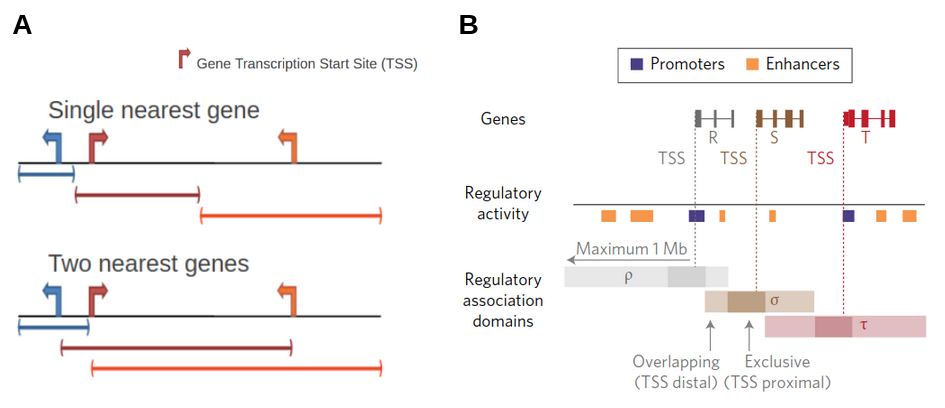
\includegraphics[width=1\textwidth, page=1]{figures/chap2/chap2-fig1.png}
    \caption[Approches d'association entre gène et élément \textit{cis}-régulateur par voisinage.]{
    \textbf{Approches d'association entre gène et élément \textit{cis}-régulateur par voisinage.}
    Pour chaque site d'initiation de la transcription (\acrshort{TSS}), un domaine régulateur est défini de sorte à ce que l'ensemble des éléments \gls{cis}-régulateur y étant inclus lui soit associé.
    \textbf{A.} Approche la plus simple où un élément \gls{cis}-régulateur est associé au \acrshort{TSS} (flèche) le plus proche. Les domaines régulateurs des \acrshort{TSS} (fragments colorés) ne peuvent pas se chevaucher.
    \textbf{B.} Les frontières du domaine régulateur d'un \acrshort{TSS} sont délimitées par les positions des \acrshort{TSS} voisins. Un élément \gls{cis}-régulateur est associé aux deux gènes les plus proches en amont et en aval.
    \textbf{C.} Pour chaque \acrshort{TSS}, un domaine de régulation proximal exclusif est défini, puis étendu jusqu'aux frontières des domaines proximaux des \acrshort{TSS} voisins. Une distance maximale de chaque côté du \acrshort{TSS} peut-être définie, ici 1Mb. A et B sont tirées de l'interface web de GREAT \citep{mclean_great_2010}, C est tiré de \citep{berthelot_complexity_2018}.  \\
    }
    \label{fig:chap2-fig1}
\end{figure} 

Une limitation importante de cette approche est que le nombre d’éléments \gls{cis}-régulateurs attribué à un gène est fortement dépendant de la taille de la région qui le sépare des promoteurs des gènes voisins \citep{taher_variable_2009}. Un gène isolé par de grandes régions intergéniques aura une plus forte probabilité d’être associé avec un nombre élevé d’éléments \gls{cis}-régulateurs. A l’inverse, un gène présent dans une région avec une forte densité de gènes se verra associer un “domaine de régulation” plus restreint. Par exemple, dans le cas des groupements des gènes du développement (tels que les gènes Hox et Evx) bordés par de grandes régions intergéniques souvent nommé "désert de gène”, les gènes situés aux extrémités du groupe pourront être associés avec de très nombreux éléments \gls{cis}-régulateurs \citep{taher_variable_2009}. Cette hétérogénéité de l’organisation des gènes pointe un paramètre confondant important dans la définition des paysages \gls{cis}-régulateurs par une simple approche de voisinage.

\section{Corrélation d’activité entre promoteur et régions régulatrices}
\label{sec:correl-act}

Au cours des 20 dernières années, de nombreux exemples de relations entre gènes et éléments \gls{cis}-régulateurs distaux sont venus défier le modèle d’une régulation exclusivement par voisinage immédiat dans le génome linéaire. Comme évoqué tout au long du chapitre précédent, le gène \gls{SHH} est par exemple régulé par l’amplificateur \acrshort{ZRS} situé dans un intron d’un autre gène à une distance de plus de 800 kb \citep{lettice_long-range_2003}. Un autre exemple est celui de la régulation de l’expression de cinq gènes codants pour plusieurs formes de globulines chez l’humain. Plusieurs amplificateurs situés dans une même région à seulement quelques dizaines de kilobases contrôlent l’expression de ces gènes (Figure \ref{fig:chap2-fig2}) \citep{levings_human_2002}. Selon le tissu et le stade de développement, différents gènes de globulines sont exprimés. Les amplificateurs ne sont alors pas nécessairement associés à l’unique gène le plus proche et peuvent ainsi franchir plusieurs gènes. Selon les modèles d’association par voisinage, un élément \gls{cis}-régulateur est rarement associé à plus de deux gènes (un en amont et un en aval). Dans cet exemple, les amplificateurs auraient été associés au premier gène de e-globuline et à un éventuel gène en amont. De plus, dans les cas de regroupement de gènes, comme celui ci mais aussi dans celui les gènes HoxD contrôlés par la région GCR, plusieurs gènes peuvent être régulés par des éléments \gls{cis}-régulateurs communs \citep{spitz_global_2003}. 

\begin{figure}[h]
    \centering
    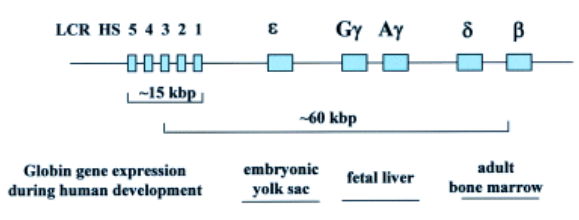
\includegraphics[width=0.8\textwidth, page=1]{figures/chap2/chap2-fig2.png}
    \caption[Schéma de l'organisation génomique des gènes de globulines et de leurs éléments \textit{cis}-régulateurs chez l'humain.]{
    \textbf{Schéma de l'organisation génomique des gènes de globulines et de leurs éléments \textit{cis}-régulateurs chez l'humain.}
    Cinq gènes de globulines sont représentés ainsi que la région LCR ("Locus Control Region") d'environ 15 kilobase contenant cinq éléments \textit{cis}-régulateurs de leur expression. Au cours du développement chez l'humain, le gène e-globuline est exprimé au cours du premier trimestre dans les cellules érythroïdes dérivées de l'hématopoïèse du sac vitellin. Les gènes G-gamma et A-gamma-globulines sont exprimés dans les cellules érythroïdes dans le foie foetal jusqu'à la naissance. Le gène de la bêta-globine est exprimé principalement chez l'adulte dans les cellules dérivées de l'hématopoïèse de la moelle osseuse.
    Les distances ne sont pas à l'échelle. Tiré de \citep{levings_human_2002}\\
    }
    \label{fig:chap2-fig2}
\end{figure} 

L’utilisation des premières données de contact de la chromatine ciblées sur certains loci ont montré que les promoteurs des gènes en interaction physique avec les mêmes régions régulatrices ont tendance à être co-exprimés à travers plusieurs échantillons \citep{dekker_capturing_2002, chepelev_characterization_2012, li_extensive_2012}. Motivé par cette corrélation et surtout par la découverte de la transcription des amplificateurs \citep{kim_widespread_2010}, il a alors été proposé d’utiliser les mesures de l’activité des promoteurs et des amplificateurs pour déterminer leurs associations (cf Chapitre 1 \ref{subsubsec:eRNA}). Par exemple, en utilisant la corrélation de la quantité de transcrits bidirectionnels de chaque paire de promoteur et d’amplificateur à travers plusieurs échantillons, il a été estimé que seuls 40\% des amplificateurs sont associés avec le promoteur le plus proche \citep{andersson_atlas_2014}. Cependant, bien que certaines méthodes existent pour prendre en considération des modèles de co-activité non linéaire \citep{hait_focs_2018}, ces corrélations ne peuvent identifier des interactions régulatrices complexes, par exemple où un gène est régulé par de nombreux amplificateurs optionnels et redondants. Il est également difficile par cette méthode de détecter les paires gène-amplificateur spécifiques d’un type cellulaire, particulièrement lorsqu’un gène est pléiotropique mais qu’une partie de ses éléments \gls{cis}-régulateurs sont spécifiques. Plusieurs autres méthodes de corrélation exploitent l’accumulation des marques de chromatine caractéristiques de l’activité des gènes et des éléments \gls{cis}-régulateurs \citep{whalen_enhancerpromoter_2016, cao_reconstruction_2017}. Celles-ci nécessitent de très nombreuses données pour modéliser et prédire les associations entre gène et amplificateur selon les modifications de la chromatine.  

\section{Mesure des contacts de la chromatine}
\label{sec:mesure-contact}

Les techniques de capture de la conformation de la chromatine permettent de mesurer expérimentalement les contacts (ou la proximité physique) entre des régions du génome. Les premières cartes de contacts de la chromatine à l’échelle du génome complet ont ainsi révélé une structure complexe où de nombreux loci distants se rapprochent spatialement par des boucles d’ADN \citep{schoenfelder_pluripotent_2015, mifsud_mapping_2015}. La vision tridimensionnelle permettrait alors de s’affranchir de la notion de distance linéaire entre les séquences pour déterminer les associations régulatrices. La technique de capture de conformation de la chromatine ciblée sur les promoteurs des gènes (\gls{PCHi-C}, cf Chapitre1 \ref{subsec:HiC}), ouvre aujourd’hui la possibilité de définir plus précisément le paysage \gls{cis}-régulateur de chaque gène. \\

Un de mes premiers objectifs de thèse a été de rassembler l’ensemble des données de \gls{PCHi-C} disponibles à l’échelle génomique. J’ai ainsi récupéré les données brutes de séquençage de 12 publications, recoupant 26 échantillons provenant de 16 types cellulaires pour l’humain \citep{choy_promoter_2018, freire-pritchett_global_2017, javierre_lineage-specific_2016, mifsud_mapping_2015, pan_integration_2018, rubin_lineage-specific_2017}. J’ai ensuite mis en place un traitement bio-informatique pour traiter de façon homogène l’ensemble de ces données pour déterminer les contacts de chromatine. Pour évaluer la présence de contacts potentiellement régulateurs, j’ai utilisé les prédictions d'éléments amplificateurs de l’expression des gènes à partir de différentes sources et types de données \citep{andersson_atlas_2014, roadmap_epigenomics_consortium_integrative_2015, hait_focs_2018}. J’ai effectué des traitements identiques à partir de données de \gls{PCHi-C} et de prédiction d’amplificateurs disponibles pour la souris, que j’utiliserai dans les parties suivantes \citep{comoglio_thrombopoietin_2018, koohy_genome_2018, novo_long-range_2018, schoenfelder_pluripotent_2015, schoenfelder_divergent_2018, siersbaek_dynamic_2017}. Les détails des méthodes employées seront décrits plus amplement dans le Chapitre 3 (cf \ref{chap:chap3}) de cette thèse. Ces méthodes permettent d’obtenir une représentation des contacts de chromatine entre un fragment de restriction couvrant des régions promotrices et d’autres régions du génome qui contiennent potentiellement des éléments \gls{cis}-régulateurs (Figure \ref{fig:chap2-fig3}). De plus, afin d’obtenir un attendu aléatoire des contacts j’ai également produit des simulations pour chaque échantillon, à partir des mêmes fragments de restriction et des mêmes régions promotrices ciblées. Celles-ci tiennent compte du nombre d'interactions par région promotrice, de la distribution des distances (sur le génome linéaire) entre les régions contactées.


\begin{figure}[h]
    \centering
    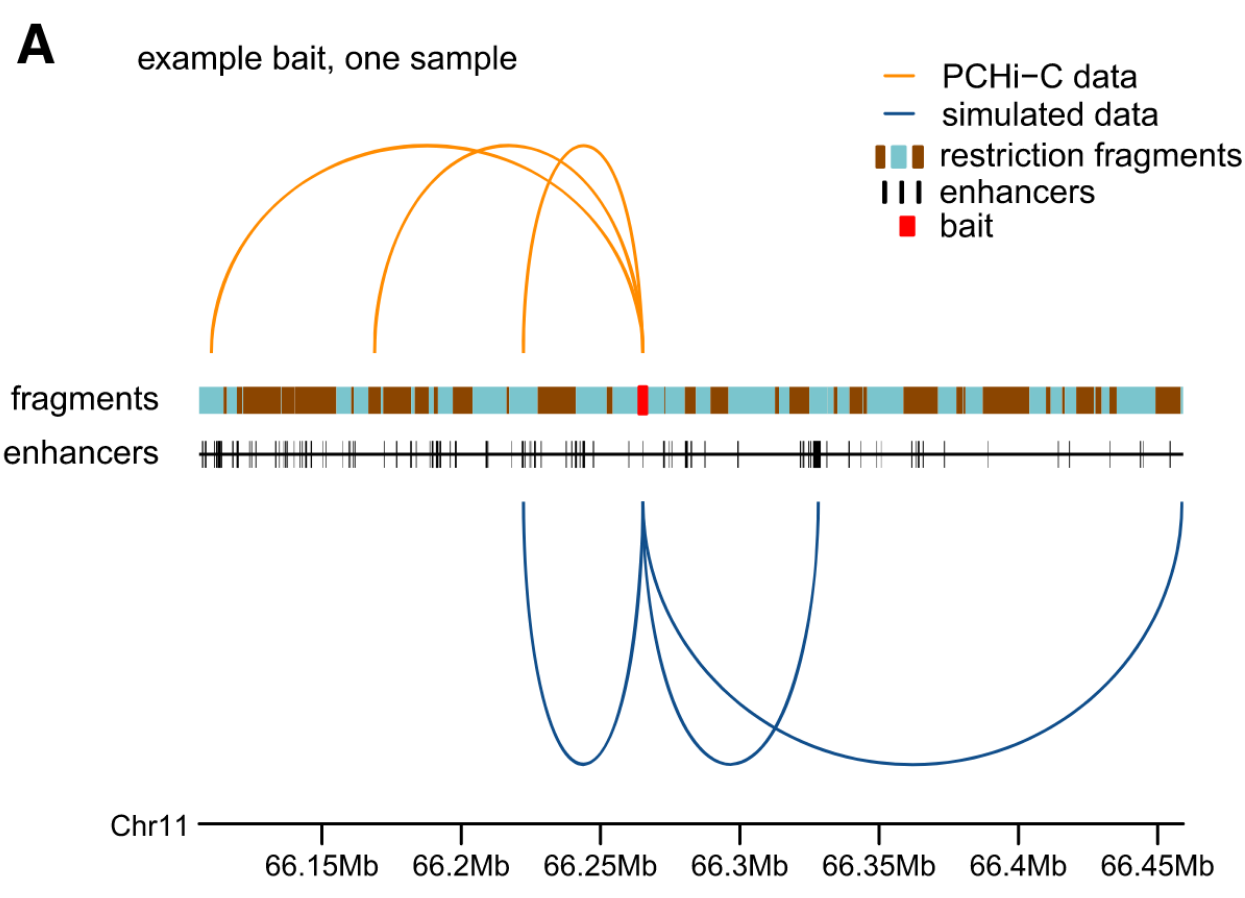
\includegraphics[width=0.8\textwidth, page=1]{figures/chap2/chap2-fig3.png}
    \caption[Contacts de chromatine mesurés par les données de \gls{PCHi-C} et par les données simulée.]{
    \textbf{Contacts de chromatine mesurés par les données de \gls{PCHi-C} et par les données simulée.} Exemple d'interactions entre un fragment de restriction ciblé enrichi en région promotrice (rouge) et d'autres fragments (bleus et marrons), d'après les données de \gls{PCHi-C} (orange) ou les données simulées (bleu). Les positions des amplificateurs ENCODE sont indiquées en noir sous les coordonées des fragments de restrictions. \\
    }
    \label{fig:chap2-fig3}
\end{figure} 

Les premières études utilisant le \gls{PCHi-C} ont montré que les contacts de chromatine sont enrichis en interactions régulatrices. Les régions contactées par les promoteurs sont enrichies en marques d’histones actives (H3K4me1, H3K27ac…) caractéristiques de la présence d’amplificateurs de l’expression \citep{schoenfelder_pluripotent_2015}. Le niveau d’expression des gènes dont les promoteurs sont en contact avec ces régions est corrélé à l’enrichissement de ces marques. De plus, les promoteurs des gènes faiblement ou non exprimés contactent des régions enrichies en marques d’histones répressives (H3K27me3) et pauvres en marques actives. Les gènes contactent ainsi des régions présentant des marques d’histones qui semblent appropriées à leur état d’activité. Les régions contactées sont également enrichies en protéines et facteurs de transcription fixés à la chromatine et associés au niveau d’expression des gènes (RNAPII, CTCF, …) \citep{javierre_lineage-specific_2016}.\\

Nous avons confirmé cet enrichissement en relations régulatrices dans les données combinées de \gls{PCHi-C} (cf Chapitre 3 \ref{chap:chap3})) \citep{laverre_long-range_2022}. Notamment, les régions contactées contiennent une proportion significativement plus grande d’amplificateurs qu’attendu par hasard (Figure \ref{fig:chap2-fig4}.A). La proportion d’amplificateur diminue lorsque la distance aux promoteurs augmente, ce qui pourrait être cohérent avec un modèle de régulation limité à une certaine distance où la majorité des relations régulatrices auraient lieu à proximité des gènes (Figure \ref{fig:chap2-fig4}. C). De plus, nous avons observé une plus grande co-activité des paires gène-amplificateur contactées en \gls{PCHi-C} que dans les données simulées, où la corrélation diminue fortement avec la distance (Figure \ref{fig:chap2-fig4}. B). Les contacts de chromatine mesurés par \gls{PCHi-C} peuvent donc fournir une information pertinente du paysage \gls{cis}-régulateur et permettre une inférence des gènes cibles des éléments \gls{cis}-régulateurs.

\begin{figure}[H]
    \centering
    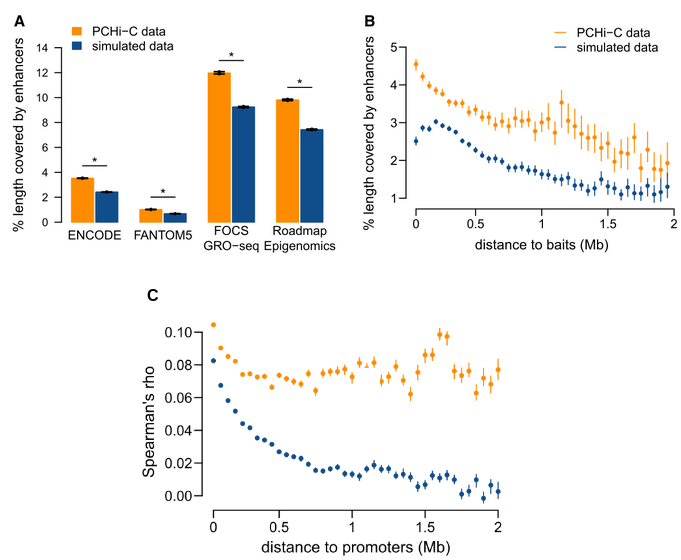
\includegraphics[width=1\textwidth, page=1]{figures/chap2/chap2-fig4.png}
    \caption[Les contacts de chromatine detéctés par \gls{PCHi-C} sont enrichis en relations regulatrices.]{
    \textbf{Les contacts de chromatine detéctés par \gls{PCHi-C} sont enrichis en relations regulatrices.}
    \textbf{A.} Proportion moyenne de la longueur couverte par les amplificateurs prédits par plusieurs méthodes pour les régions génomiques contactées dans les données de \gls{PCHi-C} chez l'humain (orange) et dans les données de contacts simulées (bleu). 
    \textbf{B.} Proportion moyenne de la longeur couverte par des amplificateurs prédits par le consortium ENCODE selon la distance génomique entre les régions promotrices et les régions contactées. 
    \textbf{C.} Distribution des coefficients de Spearman entre les niveaux d'activité des promoteurs et des amplificateurs prédits par ENCODE selon la distance génomique qui les sépare pour les associations déterminées par les données de \gls{PCHi-C} et les données simulées. Les segments verticaux représentent les intervalles de confiance à 95\% de la moyenne. (*) indique une différence significative entre les données de \gls{PCHi-C} et les données simulées (FDR $<$ 10e-10) selon un test de chi2.
    Tirées de \citep{laverre_long-range_2022}.
    }
    \label{fig:chap2-fig4}
\end{figure} 

\section{Comparaison d’une approche de voisinage et des contacts de la chromatine}
\label{sec:comp-voisinage-contact}

L’approche par voisinage étant la plus couramment utilisée, nous avons souhaité comparer les caractéristiques des paysages \gls{cis}-régulateurs des gènes déterminés par celle-ci, par rapport à ceux déterminés par les données de \gls{PCHi-C}. Nous avons ainsi défini un domaine de régulation pour chaque gène délimité par les \acrshort{TSS} des gènes voisins les plus proches en amont et en aval. Chaque amplificateur situé dans cette zone a été attribué au gène. Dans les deux approches, nous avons considéré uniquement les amplificateurs situés à une distance maximale de 2Mb du \acrshort{TSS} des gènes codants pour des protéines. Tous les gènes ne sont pas représentés dans les données de \gls{PCHi-C} car seules certaines régions promotrices sont ciblées par le protocole expérimental. Elles contiennent 70\% (15,702 sur 22,686) des \acrshort{TSS} de gènes codants pour des protéines chez l’humain. 

\subsection{Complexité des paysages \textit{cis}-régulateurs prédits}
\label{subsec:complexité-predit}

Dans un premier temps nous avons analysé les différences de complexité, définie par le nombre d’amplificateurs, des paysages \gls{cis}-régulateurs des gènes dans chacune des approches. Le nombre d’amplificateurs attribué aux gènes est plus grand dans les données de \textbf{contact de chromatine} (médiane = 17) que par une association par \textbf{voisinage} (médiane = 11) (Figure \ref{fig:chap2-fig5}.A). Pour les gènes associés à au moins un amplificateur par les deux approches (N=12,553), les différences du nombre d’amplificateur sont très variables mais l’approche par \gls{PCHi-C} attribue en moyenne plus d’amplificateur par gène (Figure \ref{fig:chap2-fig5}.C, différence moyenne = 6.89). De plus, les complexités des paysages \gls{cis}-régulateurs évalués avec les deux méthodes sont faiblement corrélées (rho de Spearman=0.18; p-value $<$ 2.2e-16). Les données de \textbf{\gls{PCHi-C}} prédisent ainsi un nombre plus important de paires gène-amplificateur (425,168) que l’approche par \textbf{voisinage} (338,644). Comme attendu, ces paires franchissent des distances génomiques significativement plus grandes dans les données \gls{PCHi-C} (médiane = 269 kb) qu’avec une approche de voisinage (médiane = 49 kb; test de Wilcoxon p-value $<$10e-10) (Figure \ref{fig:chap2-fig5}.B). Ceci s’explique en partie par le fait que les contacts de chromatine entre des régions séparées par une distance de moins de 25 kb sont exclus de l’analyse en \gls{PCHi-C}, là où sont présentes 34\% des paires prédites par voisinage. En effet, en raison de la plus grande probabilité d’observer des régions en proximité physique dans le noyau lorsque celles-ci sont voisines sur le génome linéaire, il est difficile d’estimer avec fiabilité la proportion de contacts régulateurs à moins de 25 kb \citep{cairns_chicago_2016}. Dans l’intervalle de distance 25 kb-2 Mb, 43,940 paires gène-amplificateur sont prédites en commun par les deux approches. Du point de vue des contacts \textbf{\gls{PCHi-C}}, ces paires communes sont majoritairement celles séparées par une courte distance génomique (37\% de paires en commun entre 25 et 75 kb) et cette proportion diminue très rapidement pour être inférieure à 5\% à partir de 250kb. Du point de vue des paires gène-amplificateur définies par le \textbf{voisinage}, on observe une diminution de paires en commun avec la distance, mais on note une augmentation pour les distances les plus grandes. Les paires prédites par \textbf{voisinage} à plus de 1Mb sont composées de gènes séparés par de très grandes régions intergéniques.\\

\begin{figure}[H]
    \centering
    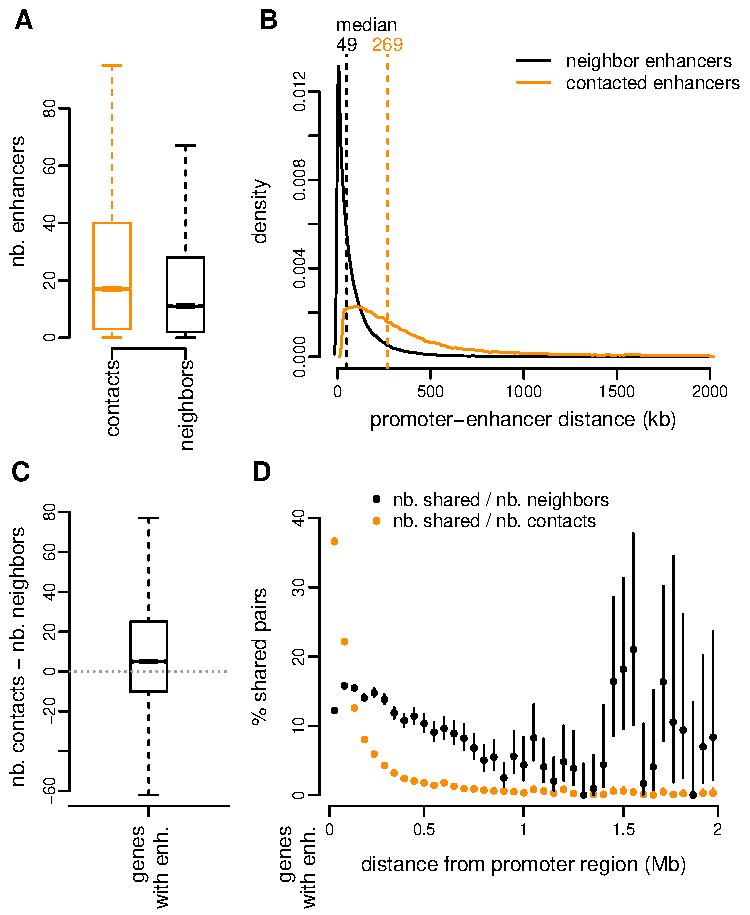
\includegraphics[width=0.7\textwidth, page=1]{figures/chap2/chap2-fig5.pdf}
    \caption[Comparaisons des associations entre gène et amplificateurs inférées par les données de \gls{PCHi-C} et par une approche de voisinage.]{
    \textbf{Comparaisons des associations entre gène et amplificateurs inférées par les données de \gls{PCHi-C} (orange) et par une approche de voisinage (noir).}
    \textbf{A.} Distributions du nombre d'amplificateurs attribués à chaque gène avec les données \gls{PCHi-C} ou avec l'approche de voisinage.
    \textbf{B.} Densité de la distribution des distances génomique entre les promoteurs des gènes et les amplificateurs, pour les deux approches. 
    \textbf{C.} Distribution de la différence du nombre d'amplificateurs attribués à chaque gène avec l'approche \gls{PCHi-C} et l'approche de voisinage. 
    \textbf{D.} Pourcentage de paires gène-amplificateur partagées entre les deux approches, en fonction de la distance génomique entre les promoteurs et les amplificateurs.
    }
    \label{fig:chap2-fig5}
\end{figure} 

\subsection{Taille des domaines de régulation}
\label{subsec:taille-domaine}

Nous avons ensuite évalué la relation entre la taille du domaine de régulation et la complexité des paysages \gls{cis}-régulateurs. Pour l’approche de \textbf{voisinage}, la taille du domaine de régulation, qui est majoritairement déterminée par la distance aux \acrshort{TSS} voisins, est corrélée positivement au nombre d’amplificateurs qui lui sont attribués (Figure \ref{fig:chap2-fig6}.A; rho de Spearman=0.73 ; p-value $<$ 2.2e-16). Les gènes associés à de nombreux amplificateurs voisins sont enrichis pour des fonctions associées à des processus du développement (Figure \ref{fig:chap2-fig6}.B). La taille du domaine défini pour l'approche de \textbf{voisinage} est peu corrélée au nombre d’amplificateurs associés aux gènes par \gls{PCHi-C}, qui reste en moyenne à 15 amplificateurs par gène (rho de Spearman= -0.04; p-value $<$ 6.1e-6). Par contre, la taille du domaine de contact d’un gène définie par la somme des longueurs des régions contactées en \gls{PCHi-C}, est fortement corrélée avec le nombre d’amplificateurs qui lui sont attribués (rho de Spearman= 0.72 ; p-value $<$ 2.2e-16). Il est intéressant de noter qu’il n'existe qu’une faible corrélation entre la taille du domaine \textbf{voisin} et la taille du domaine \textbf{contacté} (rho de Spearman= 0.04 ; p-value $<$ 1.1e-5). Ceci indique notamment que le nombre d’amplificateur associé à un gène dépend du nombre et de la taille des régions \textbf{contactées} mais pas du \textbf{voisinage} du gène. Les gènes associés à de nombreux amplificateurs selon les données de PCHi-C sont enrichis en fonctions de régulation de processus métabolique (Figure \ref{fig:chap2-fig6}.C).

\begin{figure}[H]
    \centering
    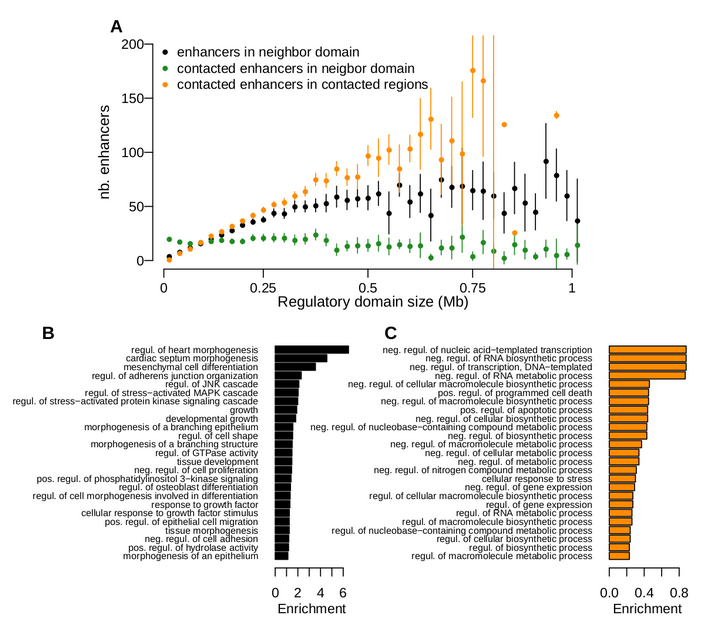
\includegraphics[width=0.9\textwidth, page=1]{figures/chap2/chap2-fig6.png}
    \caption[Attribution des amplificateurs aux gènes cibles selon les domaines de régulation.]{
    \textbf{Attribution des amplificateurs aux gènes cibles selon les domaine de régulation.}.
    \textbf{A.} Nombre moyen d'amplificateur attribué aux gènes selon la taille du domaine régulateur défini par une approche de voisinage (noir) ou par les contacts de chromatine mesurés par \gls{PCHi-C} (orange). Le nombre moyen  d'amplificateur contacté par les gènes en \gls{PCHi-C} et à la fois présent dans les domaines régulateurs défini par voisinage est representé en vert. 
    \textbf{B.} Enrichissement ontologique des gènes triés par ordre décroissant du nombre d'amplificateur leur étant attribué par l'approche de voisinage. Seuls les 25 termes les plus enrichis sont montrés (FDR $<$ 10e-5).
    \textbf{C.} Idem que B. pour les amplificateurs attribués dans les données de \gls{PCHi-C}.
    }
    \label{fig:chap2-fig6}
\end{figure}

\subsection{Relation entre nombre d’amplificateur et expression des gènes}
\label{subsec:complexite-expression}

Nous avons ensuite évalué la relation entre les paysages \gls{cis}-régulateur prédits par les deux approches et le patron d’expression des gènes dans plusieurs organes et stades de développement \citep{cardoso-moreira_gene_2019}. Nous avons mesuré le niveau moyen d’expression des gènes ainsi que l’étendue de l’expression d’un gène, une mesure du nombre d'échantillons dans lequel le gène est exprimé \citep{laverre_long-range_2022}. Nous confirmons que le niveau d’expression des gènes est positivement associé avec le nombre d’amplificateurs \textbf{contactés} dans les données de \gls{PCHi-C} (Figure \ref{fig:chap2-fig7}. A; test de Kruskal–Wallis, p-value $<$ 10-10) \citep{javierre_lineage-specific_2016}. Ceci est en accord avec le rôle activateur de l’expression des amplificateurs avec un effet additif important \citep{schoenfelder_pluripotent_2015, mifsud_mapping_2015}. On observe aussi une forte relation entre le nombre d’amplificateurs \textbf{contactés} et l’étendue de l’expression des gènes (Figure \ref{fig:chap2-fig7}.B; test de Kruskal–Wallis, p-value $<$ 10-10). Plus un gène possède d’amplificateurs et plus celui-ci est actif dans un grand nombre d'échantillons, ce qui ne semble pas être le cas pour le nombre d’amplificateurs \textbf{voisins}. Cependant, contrairement à certaines études nous n’observons pas de relation entre l’expression des gènes et le nombre d’amplificateurs \textbf{voisins}. Cette différence peut s’expliquer par le fait que nous ne tenons pas compte de l’activité des amplificateurs au sein de chaque échantillon dans aucune des deux approches. En considérant seulement les amplificateurs \textbf{voisins} actifs dans le même tissu où l’expression des gènes est mesurée, l’estimation de l’ensemble du paysage \gls{cis}-régulateur d’un gène permet d’observer une relation avec le niveau d’expression \citep{berthelot_complexity_2018}.\\

\begin{figure}[h]
    \centering
    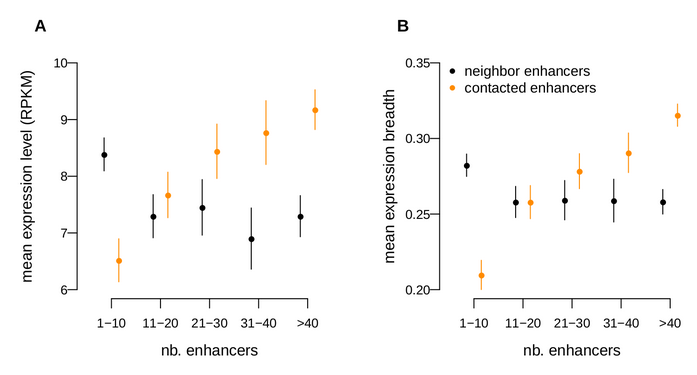
\includegraphics[width=0.8\textwidth, page=1]{figures/chap2/chap2-fig7.png}
    \caption[Relations entre le nombre d'amplificateurs et l'expression des gènes.]{
    \textbf{Relations entre le nombre d'amplificateurs et l'expression des gènes}. Les amplificateurs sont attribués aux gènes selon une approche de voisinage (noir) ou selon les données de contact de chromatine identifés par \gls{PCHi-C} (orange).
    \textbf{A.} Niveau moyen d'expression des gènes selon le nombre d'amplificateur attribués.
    \textbf{B.} Etendue du niveau de l'expression selon le nombre d'amplificateur.
    L'expression des gènes est mesurée sur plusieurs organes et stades de développement d'après les données de \citep{cardoso-moreira_gene_2019} (cf Méthodes dans la Partie \ref{part:chap3}).
    }
    \label{fig:chap2-fig7}
\end{figure} 

Bien qu’il s’intersectent dans une certaine mesure, les paysages \gls{cis}-régulateurs des gènes sont ainsi très différents lorsqu’ils sont définis selon une approche d’association par voisinage ou par les données de contact de chromatine. Le nombre absolu d’amplificateurs par gène n’est pas fortement corrélé entre les méthodes et ceux-ci sont surtout situés à des distances génomiques très différentes par rapport aux promoteurs. Les gènes auxquels on attribue de nombreux amplificateurs sont très différents selon les approches. Cette comparaison a confirmé que les contacts de chromatine ne mettent généralement pas en interaction les gènes et les amplificateurs directement voisins. La distance entre les \acrshort{TSS} voisins (qui dépend de la taille des régions intergéniques ainsi que de la longueur totale des gènes) est le facteur principal de la complexité du paysage \gls{cis}-régulateur d’un gène par l’approche de voisinage. L’organisation du génome est donc un facteur majeur dans l’attribution des éléments \gls{cis}-régulateurs aux gènes avec cette approche. Les contacts de chromatine semblent quant à eux être indépendants de l’organisation génomique unidimensionnelle, c’est-à-dire de la répartition des gènes sur le génome linéaire. Il existe des biais dans les deux méthodes, qui peuvent aller dans des directions opposées. Par exemple, l’approche par \gls{PCHi-C} n’est pas en capacité d’inférer des interactions à très courtes distances (inférieure à 25kb) qui pourraient avoir une grande importance fonctionnelle. De plus, elle ne permet pas de distinguer avec précision les relations régulatrices entre des contacts mettant en relation des régions contenant plusieurs promoteurs ou amplificateurs proches. Ces observations soulignent la complexité de la définition des paysages \gls{cis}-régulateurs de l’expression des gènes. Aucune approche ne semble parfaite mais les données de contacts de la chromatine peuvent permettre d’apporter un nouveau regard sur les relations régulatrices et aider à mieux comprendre les déterminants génétiques de l’expression des gènes. 


\section{Inférer les fonctions biologiques des éléments \textit{cis}-régulateurs}
\label{sec:inferer-fonction}

Pour de nombreuses études, prédire les rôles biologiques d’un ensemble d’éléments \gls{cis}-régulateurs (par exemple, ceux qui sont actifs dans un certain tissu ou stade de développement, ceux qui sont fixés par une protéine d’intérêt, ceux qui changent d’activité suite à une manipulation génétique, etc.) peut être crucial. Pour cela, une des méthodes les plus largement utilisées est de transférer les annotations fonctionnelles (telles que les annotations Gene Ontology, participation à des voies de signalisation etc.) des gènes aux éléments \gls{cis}-régulateurs qui leur sont associés. Afin de prédire les fonctions préférentiellement associés à un ensemble d’éléments \gls{cis}-régulateurs, il est possible d’effectuer un test d’enrichissement à partir de ces annotations fonctionnelles. L’outil GREAT est très fréquemment utilisé pour effectuer cette tâche \citep{mclean_great_2010}. Celui-ci utilise une approche de voisinage pour associer les éléments \gls{cis}-régulateurs à leurs gènes cibles, comme décrit au-dessus. Dans la variante “par défaut” de GREAT, chaque gène se voit attribuer un domaine de régulation proximal et un domaine de régulation élargi, qui peut s’étendre jusqu’au domaine proximal des gènes voisins dans une certaine limite de distance. Comme précédemment mentionné, la taille des domaines de régulation définis de cette manière dépend de la fonction des gènes. Par exemple, les gènes impliqués dans les processus développementaux ont des domaines de régulation plus grands que les autres \citep{mclean_great_2010}. Dans GREAT ce biais est correctement pris en compte. Pour ce faire, l’attendu par hasard pour chaque annotation fonctionnelle est déterminé par la taille cumulée des domaines régulateurs des gènes associés à cette annotation fonctionnelle. Cette prise en compte de l’organisation génomique permet à GREAT de prédire des fonctions pour les éléments \gls{cis}-régulateurs. Les fonctions prédites ont un sens biologique, étant donné le contexte dans lesquels ces éléments ont été détectés \citep{mclean_great_2010, rada-iglesias_unique_2011}. Cependant, nous avons vu que les gènes associés aux amplificateurs peuvent être différents entre l’approche d’association par voisinage et par les contacts de chromatine. Par exemple, les gènes associés à un grand nombre d’amplificateurs ne possèdent pas les mêmes fonctions entre les méthodes. Nous avons alors souhaité évaluer les conséquences de l’utilisation de ces deux méthodes sur l’attribution de fonctions biologiques aux éléments \gls{cis}-régulateurs. Pour cela nous avons développé GOntact, un outil qui utilise les contacts de la chromatine centrés sur les promoteurs pour déterminerdes enrichissements d’annotations fonctionnelles  pour des ensembles d’éléments \gls{cis}-régulateurs.

    \chapter{Article 1 - GOntact: using chromatin contacts to infer Gene Ontology enrichments for \textit{cis}-regulatory elements}
\label{GOntact}

\begin{center}
    \large Alexandre Laverré$^{\text{1}}$, Eric Tannier$^{\text{2}}$, Philippe Veber$^{\text{1}}$, Anamaria Necsulea$^{\text{1}}$\\
    \vspace{0.5cm}
    \normalsize
    $^{\text{1}}$Univ Lyon, Université Claude Bernard Lyon 1, CNRS, Laboratoire de Biométrie et Biologie Evolutive, F-69100, Villeurbanne, France.\\
    $^{\text{2}}$Centre de recherche Inria de Lyon, 69603 Villeurbanne, France\\
\end{center}

{\hypersetup{linkcolor=GREYDARK}\minitoc}

\section{Abstract}
While the genomic positions and the patterns of activity of enhancer elements can now be efficiently determined, predicting their target genes remains a difficult task. Although chromatin conformation capture data has revealed numerous long-range regulatory interactions between genes and enhancers, enhancer target genes are still traditionally inferred based on genomic proximity. This approach is at the basis of GREAT, a widely used tool that aims to analyze the functional significance of sets of \acrshort{cis}-regulatory elements. Here, we propose a new tool, named GOntact, which infers regulatory relationships using promoter-capture Hi-C (PCHi-C) data and uses these predictions to derive Gene Ontology enrichments for sets of \acrshort{cis}-regulatory elements. We apply GOntact on enhancer and PCHi-C data from human and mouse and show that it generates functional annotations that are coherent with the patterns of activity of enhancers. We find that there is substantial overlap between functional predictions obtained with GREAT and GOntact but that each method can yield unique testable hypotheses, reflecting the underlying differences in target gene assignment. With the increasing availability of high-resolution chromatin contact data, we believe that GOntact can provide better-informed functional predictions for \acrshort{cis}-regulatory elements.

\section{Introduction}
In multicellular organisms, gene expression is controlled by complex interactions involving numerous trans-acting factors and \acrshort{cis}-regulatory elements. This latter class of elements, which are by definition situated on the same chromosome as the gene they regulate, can activate or inhibit gene expression (in the case of enhancers or silencers, respectively). Identifying these \acrshort{cis}-regulatory sequences at a genome-wide scale can be more or less challenging depending on the category of elements. For enhancers, their genomic positions and their patterns of activity across tissues and cell types can now be efficiently determined with various techniques, including chromatin immunoprecipitation followed by sequencing (ChIP-seq), assays for transposase-accessible chromatin using sequencing (ATAC-seq), DNAse I hypersensitivity assays (DHA) or global run-on sequencing (GRO-seq). These techniques determine the genomic localization of chromatin modifications such as histone methylation or acetylation (ChIP-seq), more generally of open chromatin regions (ATAC-seq or DHA), or the presence of nascent transcripts (GRO-seq). The presence of one or several of these epigenomic features can predict enhancer position and activity with great sensitivity. However, identifying enhancer target genes remains a difficult question, even when their localization and molecular function have been ascertained. \\

The most commonly used approach to predict enhancer target genes is the “genomic proximity” approach, which relies on the assumption that enhancers generally regulate their neighbor genes. This approach is at the basis of the GREAT software and webserver \citep{mclean_great_2010}, which uses the resulting associations between \acrshort{cis}-regulatory elements and genes to infer functional enrichments for sets of regulatory elements. This tool is extremely popular, as illustrated by the large number of scientific articles that cite it (3196 citations in Google Scholar as of March 2022). GREAT is widely used to predict functional enrichments, including but not limited to Gene Ontology enrichments, for sets of \acrshort{cis}-regulatory elements that are of interest in a given study - for example, enhancer elements that are specifically active in response to an external stimulus or in a given tissue (ref recent papers). \\ 

The assumption of genomic proximity between enhancers and target genes is undoubtedly reasonable. There is indeed evidence that most enhancers may be found within 50 kb of the genes they regulate (ref). However, the generality  of this assumption is now questioned, with mounting evidence that enhancers can be situated at large genomic distances from the genes they control (ref Shh, iroquois, some Hox work from Denis). In this case, chromatin loops bring enhancers and gene promoters in physical proximity in the nucleus. These “contacts” between different genomic regions can be detected through chromosome conformation capture (“C”) techniques (ref). With these techniques, genomic segments found in physical proximity in the nucleus are cross-linked and the chromatin is fragmented, ligated and subjected to DNA sequencing. Among the many “C” technique flavors that have been developed so far, promoter capture Hi-C (PCHi-C) and related approaches (Schoenfelder ; but also Golov 2020, Downes 2021) have been specifically designed to target chromatin contacts that involve gene promoters and other genomic regions. The resulting chromatin contact data is enriched in regulatory interactions between promoters and enhancers (same refs as above) and can thus provide a better-informed prediction of enhancer target genes. Analyses of this high-resolution, promoter-centered chromatin contact data have confirmed initial reports that enhancers do not always regulate their neighbor genes and that a substantial proportion of enhancer-promoter regulatory interactions take place at large genomic distances (refs + Laverré 2022). \\

Thus, there is overwhelming evidence that the “genomic proximity” assumption is invalidated by the presence of a large proportion of long-range regulatory interactions between enhancers and genes. In light of this, we decided to develop an alternative to the GREAT software which does not rely on this assumption. Here, we propose a new tool named GOntact, which uses PCHi-C data to infer associations between \acrshort{cis}-regulatory elements and genes, and which uses these associations to infer gene ontology enrichments for sets of regulatory elements. We apply GOntact on multiple enhancer and PCHi-C datasets from human and mouse and show that it generates functional annotations that are coherent with the patterns of activity of enhancers. We find that there is substantial overlap between functional predictions obtained with GREAT and GOntact but that each method can yield unique testable hypotheses, reflecting the underlying differences in target gene assignment. 

\section{Results}
\subsection{Target gene inference in GREAT and GOntact}

The first step towards predicting biological functions for a set of \acrshort{cis}-regulatory elements (including but not restricted to expression enhancers) is to infer (or determine) the genes whose expression they control. In GREAT, this inference is done with the traditional genomic proximity approach. With the default GREAT implementation, there are three main steps: first, genes are filtered to retain only those with relevant functional annotations (for example non-trivial Gene Ontology categories) and their canonical transcription start sites (TSS) are determined or retrieved from external sources; second, a basal regulatory domain is calculated for each gene, typically spanning 5 kb upstream and 1 kb downstream of the TSS; third, these domains are extended in both directions up to the basal  domains of the neighboring genes, within a certain maximum distance (here 1 Mb). Enhancers found within each regulatory domain are attributed to the corresponding genes (Figure \ref{fig:GOntact-fig1}.A; Methods). The number of enhancers attributed to each gene is thus determined by the size of its regulatory domain, which is itself defined by the size of the neighboring intergenic regions and by the size of the gene itself (Supplementary Figure \ref{fig:GOntact-fig1}.). The gene-enhancer associations defined by GREAT are thus directly dependent on genomic organization characteristics. \\

As an alternative to GREAT, we developed GOntact, a tool that uses high-resolution, promoter-centered chromatin interactions obtained with the PCHi-C technique (Methods) to infer regulatory relationships between enhancers and genes. We used pre-processed data from a recent publication \citep{laverre_long-range_2022}, combining 26 PCHi-C samples for human and 14 PCHi-C samples for mouse, all generated using the same protocol. The PCHi-C technique targets specifically chromatin interactions that involve gene promoters, selected using RNA baits (Methods). To further enrich for putative regulatory interactions involving promoters and enhancers, we selected chromatin contacts that take place in cis, between a baited (promoter) and an un-baited restriction fragment. For comparability with the default GREAT implementation, we impose a maximum distance of 1 Mb between the two contacting restriction fragments (Methods). The gene-enhancer pairs that are derived from PCHi-C data can be very different from those inferred with the genomic proximity approach implemented in GREAT, as illustrated for the POU6F1 human gene in Figure \ref{fig:GOntact-fig1}.. Overall, individual genes are assigned substantially more enhancers with GOntact than with GREAT (Figure \ref{fig:GOntact-fig1}.B). The median number of ENCODE enhancers assigned to a gene is 24 with GREAT and 51 with GOntact, for human (Wilcoxon rank sum, p-value $<$ 1e-10, Figure \ref{fig:GOntact-fig1}.B). The number of gene-enhancer relationships inferred by GOntact likely depends on the quality and quantity of PCHi-C data used as an input (N = 910069 interactions in total for human across 26 samples, N = 823539 for mouse across 14 samples). We restricted the number of chromatin contacts by considering only those detected in at least 2 PCHi-C samples (N = 539794 for human, N = 434305 for mouse). With this reduced dataset, the number of regulatory relationships inferred with GOntact decreases (median number of 33 enhancers per gene in the human ENCODE dataset), but remains significantly higher than the one inferred with GREAT (Wilcoxon rank sum test, p-value $<$ 1e-10, Figure \ref{fig:GOntact-fig1}.B). We note that both GREAT and GOntact assign to genes only a small fraction of the total numbers of enhancers that are present upstream and downstream of their TSS, within a maximum distance of 1 Mb (median 376 enhancers per genes, Figure \ref{fig:GOntact-fig1}.C). \\

\begin{figure}[hbt!]
    \centering
    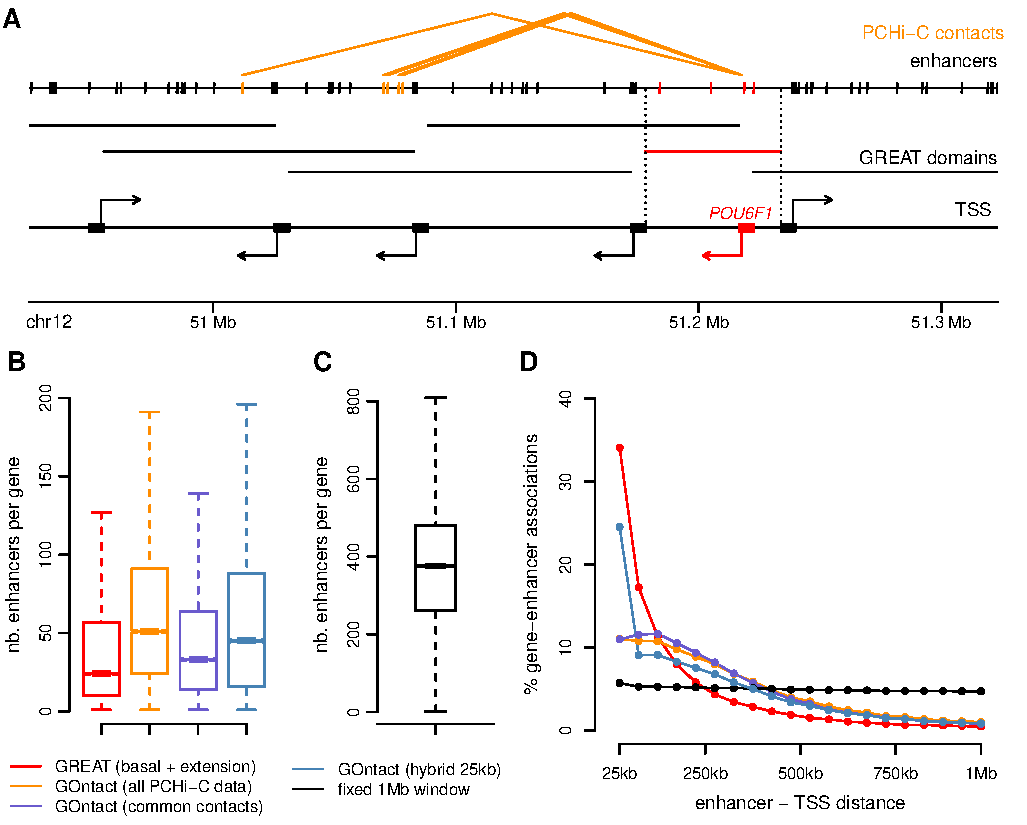
\includegraphics[width=1\textwidth, page=1] {figures/GOntact/Figure1.pdf}
    \caption[Regulatory relationships between enhancers and gene.]{
    \textbf{Regulatory relationships between enhancers and gene.}
    \textbf{A.} Illustration of the enhancer target gene predictions that underlie functional enrichment analyses in GREAT and GOntact, in a 400 kb genomic region around the human POU6F1 gene. Top: rectangles indicate the positions of ENCODE-predicted enhancers, orange lines indicate chromatin contacts between the POU6F1 gene promoter and enhancers. Middle: horizontal segments represent extended regulatory domains (up to the neighboring genes’ basal domains, within a maximum distance of 1Mb from the canonical TSS) used in GREAT. The regulatory domain and the enhancers attributed to POU6F1 by GREAT are depicted in red. Bottom: arrows depict the positions and the orientations of canonical transcription start sites (TSS) for POU6F1 and neighboring genes; black rectangles depict basal gene regulatory domains (5kb upstream, 1kb downstream of TSS) used in the default GREAT implementation.  
    \textbf{B.} Boxplots representing the numbers of enhancers assigned to genes with GREAT, with GOntact (orange: using all available PCHi-C data; purple: using chromatin contacts shared across at least 2 PCHi-C samples) or with the hybrid GOntact-GREAT approach (Methods). 
    \textbf{C.} Boxplot representing the numbers of enhancers attributed to genes with a fixed window approach (1Mb around the TSS; Methods). D. Distribution of the distances between genes and enhancers predicted to be in regulatory interactions with the GREAT, GOntact or fixed window approach. Color code as in B and C.
    \\
    }
    \label{fig:GOntact-fig1}
\end{figure} 

The genomic distances between promoters and enhancers predicted to be in regulatory interactions vary considerably among methods. With GREAT, 51\% of all gene-enhancer pairs are separated by less than 100 kb and 8\% are separated by more than 500 kb (Figure \ref{fig:GOntact-fig1}.D). With GOntact, distances between pairs of enhancers and promoters are generally larger: only 22\% are separated by less than 100 kb, and 16\% are separated by more than 500 kb (Figure \ref{fig:GOntact-fig1}.D). We note that there is an excess of enhancers situated within 50 kb of the TSS even when we define gene-enhancer pairs with a “fixed window” approach, that is, when we assign to genes all enhancers present within a maximum distance of 1 Mb of the TSS (Figure \ref{fig:GOntact-fig1}.D). In contrast, regulatory associations inferred from PCHi-C data are less frequent in close proximity to genes, which is at least in part due to the technical difficulty of distinguishing genuine from spurious chromatin contacts at small distances on the linear genome \citep{cairns_chicago_2016}. To compensate for this, we also propose a “hybrid” method that combines the principles of GREAT and GOntact: each gene is assigned a basal regulatory domain (comprising for example 25 kb upstream and 25 kb downstream of the TSS), as well as all enhancers that are in contact with its promoters in the PCHi-C data. The promoter-enhancer distance distribution for this “hybrid” approach combines features of GREAT and GOntact, as expected (Figure \ref{fig:GOntact-fig1}.D)


\subsection{Gene ontology enrichment tests}

Beyond defining putative target genes for \acrshort{cis}-regulatory elements, the aim of both GOntact and GREAT is to test for the enrichment of functional annotations associated with a set of  \acrshort{cis}-regulatory elements. Here, we apply both methods to search for enrichments of Gene Ontology (GO) annotations, in a set of enhancers. With both approaches, each enhancer is assigned all GO categories that are associated with its predicted target genes. For each GO category, we then compute the proportion of enhancers that are associated with it, among all enhancers in the dataset of interest (hereafter termed “foreground set”). We then test for an enrichment by comparing this proportion with the proportion of enhancers associated with the same GO category within a background set of elements, with a one-sided binomial test (Methods). This procedure is identical to the one implemented in GREAT, the only difference resides in the target gene assignment for enhancers. We note however that the default behavior in GREAT (at least in the web server version) is to estimate the proportion of elements associated by chance with a GO category as the cumulative size of all regulatory domains of genes that have this GO annotation, relative to the total size of the genome \citep{mclean_great_2010}. Here, we prefer to define the proportion expected by chance using a background set of enhancers, for better comparability between GREAT and GOntact. In the examples shown here, we used as a background the full set of ENCODE-predicted enhancers, which consists of 408737 elements for human and 739996 elements for mouse (ref ENCODE, Laverre 2022). As these datasets were obtained using a large number of cell types, tissues and biological conditions, we reasoned that they can provide a good estimation of what is expected at the genome-wide level for enhancer elements. 

\subsection{GOntact and GREAT functional annotations are coherent with enhancer activity patterns}

We applied GREAT and GOntact on sets of experimentally validated enhancers for human and mouse, downloaded from the Vista Enhancer Browser (ref). We analyzed sets of enhancers that are active in the embryonic heart and in the embryonic midbrain (141 and 279 enhancers for human, 170 and 166 enhancers for mouse, respectively). We evaluated GO enrichments with 5 method variations: the GREAT default “basal+extension” approach, the fixed window approach (each gene is assigned all enhancers found within a maximum 1Mb distance of its TSS), GOntact using all available PCHi-C data, GOntact using chromatin contacts observed in at least 2 PCHi-C samples and the GOntact - GREAT hybrid approach (each gene is attributed a basal regulatory domain consisting of 25 kb upstream and downstream of TSS + all enhancers in PCHi-C-defined contact with its promoter). \\

We found that all 5 methods yielded GO enrichment results that were coherent with the patterns of activity of the input enhancer datasets. For example, for embryonic heart enhancers, all methods reveal significant enrichments for GO categories related to muscle functions (Figures 2,3). Likewise, for embryonic midbrain enhancers, all 5 methods reveal significant GO enrichments related to neural differentiation (Figures 2,3). Although there is considerable overlap between the significant GO categories found by all methods (Figure \ref{fig:GOntact-fig4}.), each of them appears to prioritize a different subset of biologically relevant GO annotations. For example, for embryonic heart enhancers, GOntact methods tend to bring forward categories related to the early development of the organ (e.g., lateral mesoderm formation, embryonic heart tube elongation), whereas GREAT seems to prioritize categories related to the physiology of the embryonic and adult organ, such as the regulation of striated muscle contraction or the regulation of blood circulation (Figures 2,3). Interestingly, for embryonic midbrain enhancers, both GREAT and GOntact find stronger enrichments for processes related to gene expression regulation, rather than to brain development (Figures 2,3).

\begin{figure}[hbt!]
    \centering
    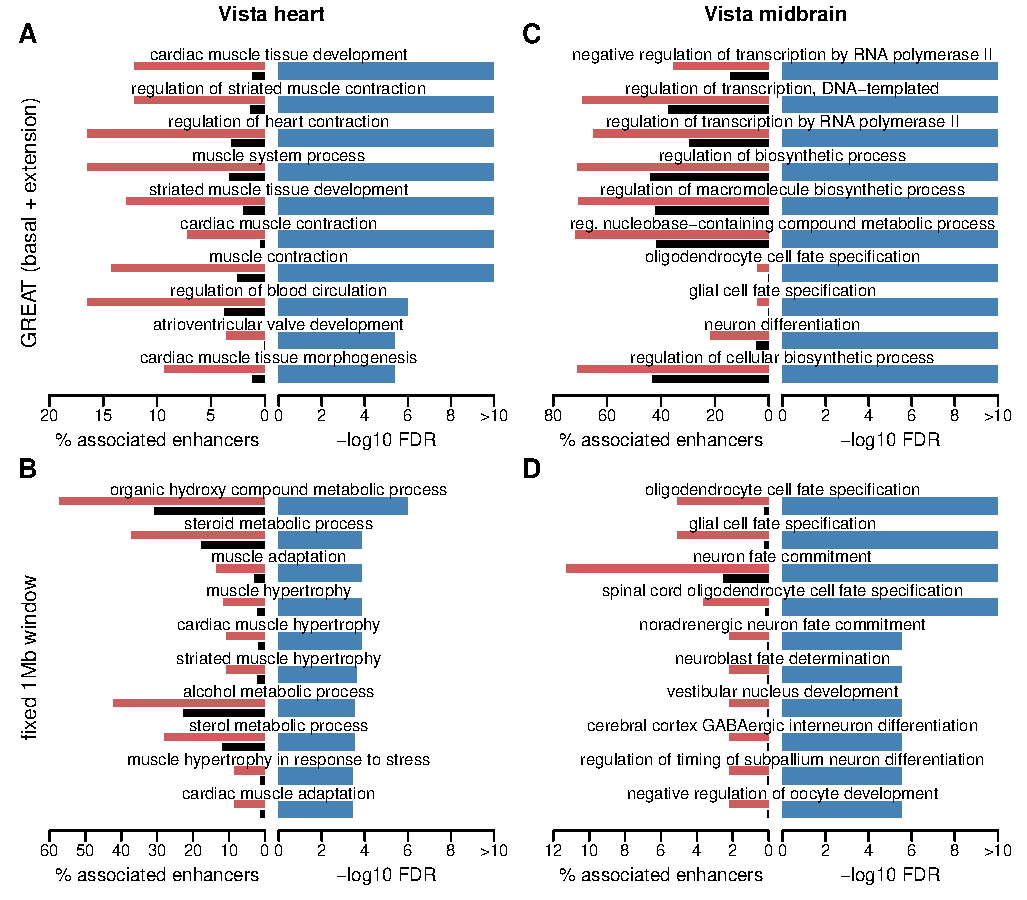
\includegraphics[width=1\textwidth, page=1] {figures/GOntact/Figure2.pdf}
    \caption[Gene Ontology Enrichment from neighboring association.]{
    \textbf{Gene Ontology Enrichment from neighboring association.}
    \textbf{A.} Gene Ontology categories that are significantly enriched (FDR $<$ 0.05, minimum enrichment 1.5, Methods) in a GREAT analysis of 141 experimentally validated human enhancers that are active in the embryonic heart (Vista), compared with a background consisting of the entire set of ENCODE-predicted enhancers. GREAT was run with default parameters: basal regulatory domain (5 kb upstream of TSS, 1 kb downstream of TSS) and an extension of a maximum 1 Mb. 
    \textbf{B.} Same as A, where enhancers are attributed to genes with a fixed 1Mb window approach (Methods). 
    \textbf{C, D.} Same as A, B for a set of 279 experimentally validated human enhancers that are active in the embryonic midbrain. 
    \\
    }
    \label{fig:GOntact-fig2}
\end{figure} 

\begin{figure}[hbt!]
    \centering
    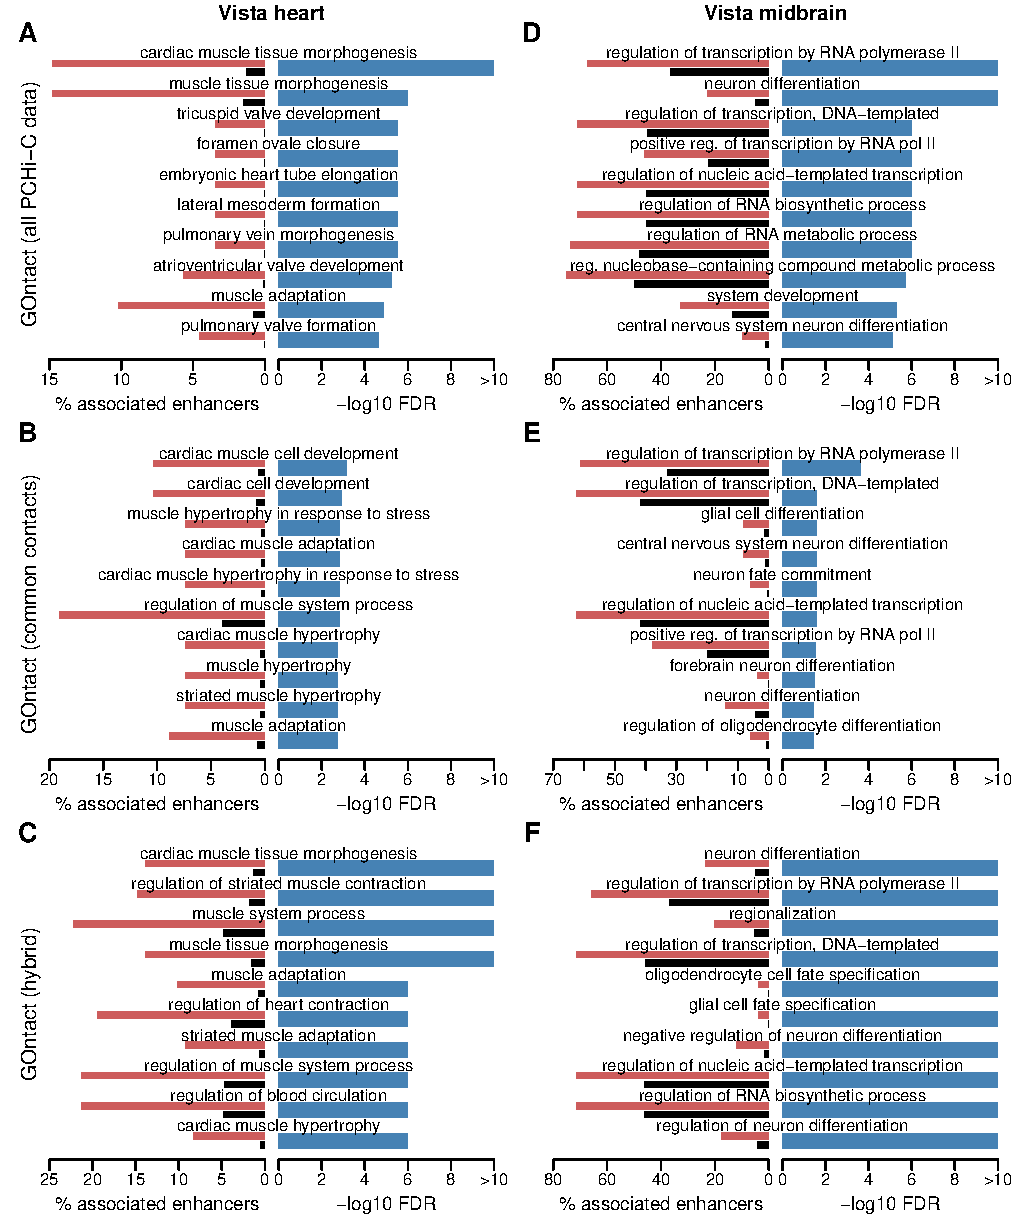
\includegraphics[width=1\textwidth, page=1] {figures/GOntact/Figure3.pdf}
    \caption[Gene Ontology Enrichment from chromatin contacts.]{
    \textbf{Gene Ontology Enrichment from chromatin contacts.}
    \textbf{A.} Gene Ontology categories that are significantly enriched (FDR $<$ 0.05, minimum enrichment 1.5, Methods) in a GOntact analysis of 141 experimentally validated human enhancers that are active in the embryonic heart (Vista), compared with a background consisting of the entire set of ENCODE-predicted enhancers. GOntact was run with all available PCHi-C data (N interactions) and a maximum distance of 1Mb was set for interactions.
    \textbf{B.} Same as A, where GOntact was run using only those interactions observed in at least 2 PCHi-C samples (N=). 
    \textbf{C.} Same as A, where GOntact was run in hybrid mode (basal domain of 25 kb upstream and downstream of TSS + chromatin contacts derived from all PCHi-C samples). 
    \textbf{D, E, F.} Same as A, B, C, for a set of 279 experimentally validated human enhancers that are active in the embryonic midbrain. 
    \\
    }
    \label{fig:GOntact-fig3}
\end{figure} 

\subsection{Enrichment of meaningful functional annotations with a simple “fixed window” approach}

Surprisingly, the simplest method used in the assignment of putative enhancer target genes (the fixed 1 Mb window approach) also reveals numerous biologically relevant GO category enrichments, at least with the enhancer datasets that we tested (Figure \ref{fig:GOntact-fig2}.). For heart enhancers, this approach reveals significant enrichments for metabolic processes, but also for muscle adaptation and muscle hypertrophy (Figure \ref{fig:GOntact-fig2}.). In fact, for this set of human enhancers, the fixed window approach is the most sensitive: it uniquely identifies more than 300 significantly enriched GO categories that are not shared with the other approaches (Figure \ref{fig:GOntact-fig4}.A). However, we note that these GO categories tend to be more general than the ones identified by the other approaches, as they are associated with a much higher proportion of background enhancers (Figure \ref{fig:GOntact-fig4}.C). For brain enhancers, the fixed window approach finds enrichments for GO categories related to the differentiation and commitment of various brain cell types (oligodendrocytes, glial cells, neurons). In this case, the fixed window approach identifies fewer  significant GO categories than the other approaches, but these categories tend to be more specific than the ones identified by the other 4 approaches, as they are associated with smaller proportions of background enhancers (Figure \ref{fig:GOntact-fig4}.D).

\begin{figure}[hbt!]
    \centering
    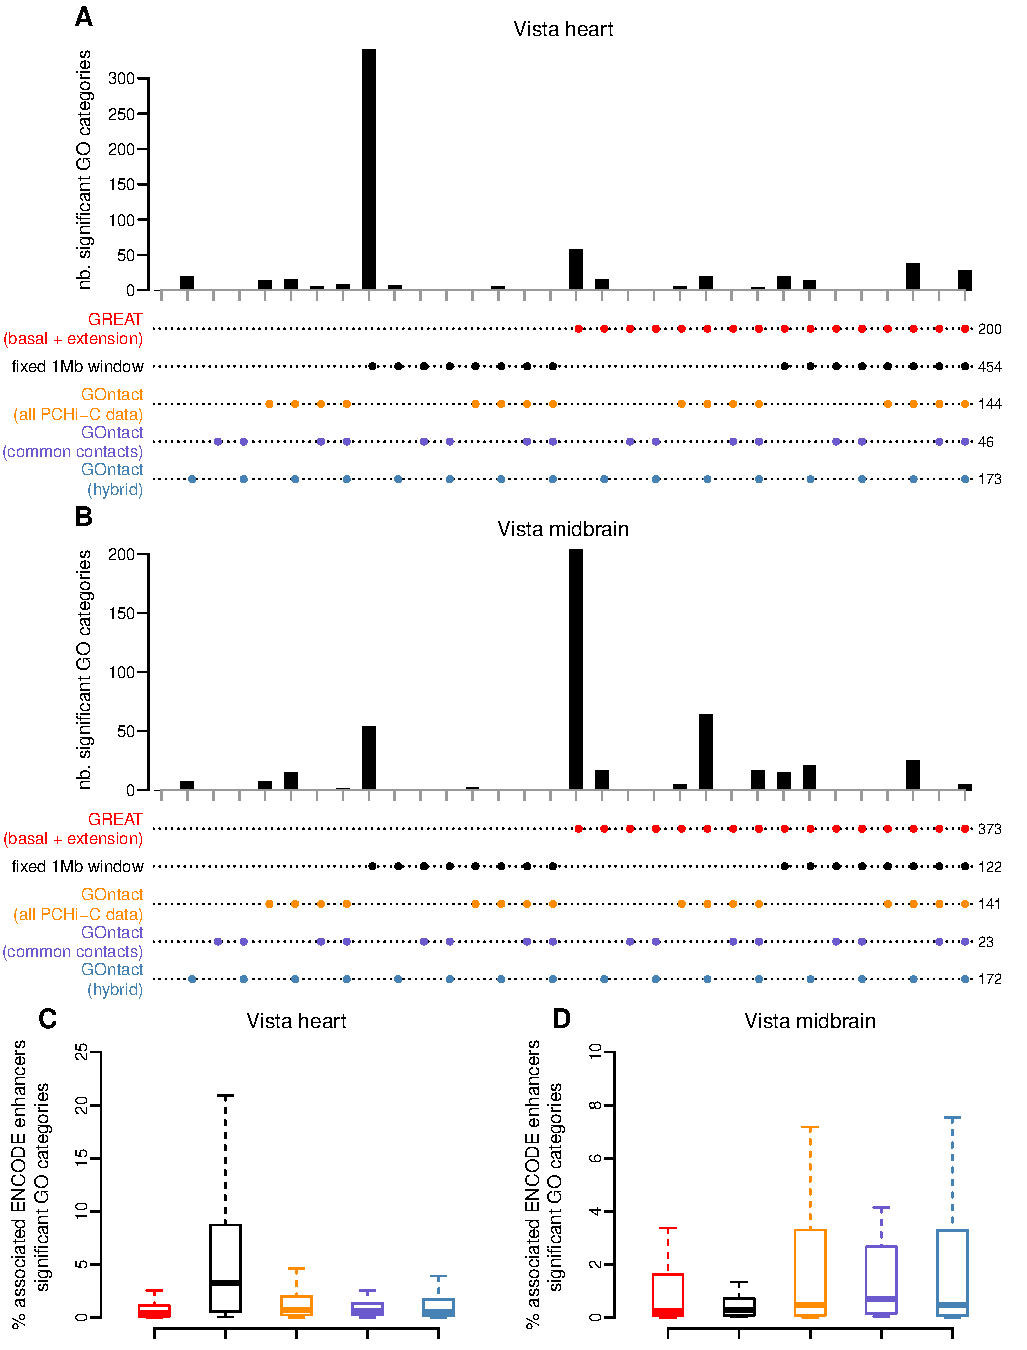
\includegraphics[width=0.8\textwidth, page=1] {figures/GOntact/Figure4.pdf}
    \caption[Comparison between Gene Ontology enrichment results obtained with different methods]{
    \textbf{Comparison between Gene Ontology enrichment results obtained with different methods :}
    \textbf{A.} GREAT (default implementation, red), fixed window (black), GOntact (using all PCHi-C data, dark orange), GOntact (using chromatin contacts observed in at least 2 PCHi-C samples, purple), GOntact hybrid mode (25 kb fixed window around TSS + chromatin contacts from all PCHi-C data, blue). The bars represent the number of significantly enriched GO categories (maximum FDR 0.05, minimum enrichment 1.5) in the 32 possible combinations of the 5 cited methods. The colored dots below the bars represent for each method whether it was included in each combination. The enrichment was computed by comparing a set of 141 experimentally validated human enhancers active in the heart with the entire ENCODE enhancer dataset. 
    \textbf{B.}  Same as A, for 279 enhancers active in the brain. 
    \textbf{C.} Boxplots depicting the proportions of ENCODE enhancers that are associated with each significantly enriched GO category, detected with the 5 methods described above. 
    \textbf{D.} Same as C,  for 279 enhancers active in the brain. 
    \\
    }
    \label{fig:GOntact-fig4}
\end{figure} 

\subsection{GOntact variants that increase sensibility and specificity}
In the default implementation of GOntact, only PCHi-C contacts are used to infer enhancer target genes. Because interactions at short genomic distances are depleted in chromatin contact data, and because there is a genuine enrichment for regulatory elements in close proximity to the gene promoter (ref), we decided to combine the principles used in the two methods into a hybrid GOntact-GREAT approach. With this approach, each gene is assigned a proximal regulatory domain (for example, 25 kb upstream and 25 kb downstream of the TSS), and all enhancers found in this domain are attributed to the corresponding gene. In addition, we add all enhancers that are connected to the gene promoter through chromatin contacts, in cis, within a maximum genomic distance (by default equal to 1 Mb). This approach efficiently combines the characteristics of GREAT and GOntact, both in terms of the distances between promoters and enhancers that are part of the inferred regulatory pairs (Figure \ref{fig:GOntact-fig1}.D), and in terms of the Gene Ontology enrichments that can be detected (Figures 2-4). The numbers of significantly enriched GO categories are indeed intermediate in the hybrid approach compared to GREAT and GOntact (Figure \ref{fig:GOntact-fig4}.) and are also coherent with the expression patterns of the selected sets of enhancers (Figure \ref{fig:GOntact-fig3}.).\\

A key factor for the success of the GOntact approach is evidently the input PCHi-C data. Ideally, chromatin contacts and \acrshort{cis}-regulatory element activity should be assessed in the same biological conditions. However, PCHi-C data is not yet available or efficiently produced for many cell types or tissues. As an alternative, we used the subset of chromatin interactions that were detected in at least two PCHi-C samples (Methods). This restricted set of interactions should be enriched in widespread (or even ubiquitous) chromatin contacts, which are likely relevant for the regulatory program of the tissue or cell type in which enhancer activity was assayed. A disadvantage is that the number of interactions that can be used is substantially reduced, which likely affects our power to detect statistically significant functional enrichments. Indeed, we found much fewer significantly enriched GO categories with this conservative variant of GOntact than with all available PCHi-C data or with the GREAT approach (Figure \ref{fig:GOntact-fig4}.). However, these functional annotations remain biologically relevant: biological processes related to cardiac cell development and muscle adaptation were found for the embryonic heart enhancers (Figure \ref{fig:GOntact-fig3}.B), and categories related to neural cell differentiation were identified for the embryonic brain (Figure \ref{fig:GOntact-fig3}.E). 

\section{Discussion}
Both GOntact and GREAT aim to predict putative biological functions for a set of \acrshort{cis}-regulatory elements of gene expression. This functional annotation can serve as a basis for further experimental validations, and can thus be seen as a source of testable hypotheses. We are indeed unable to perfectly assess the validity of our results because we lack a “golden truth”. Instead, we can only judge whether the results that we obtain are biologically meaningful, given what is known about the input dataset. Here, we applied our methods on sets of experimentally validated enhancer elements, whose pattern of activity was ascertained in mouse embryos with enhancer trap experiments (ref Vista). We thus expect an enrichment for biological processes associated with the development and the physiology of the organs in which enhancer activity was detected. Reassuringly, all the methods that we tested here show results that are coherent with these expectations, at least to some extent.  

GOntact and GREAT generally provide consistent Gene Ontology enrichment results, which is somewhat surprising given that these two methods rely on very different approaches for target gene inference. In GREAT, regulatory relationships between genes and enhancers are inferred by defining a regulatory domain for each gene, which basically always includes a proximal domain around the canonical gene TSS, and which can extend no further than the TSS of the neighboring genes, within a certain maximum genomic distance. The main assumption here is that enhancers generally regulate their neighboring genes. In GOntact, regulatory relationships are inferred based on the presence of chromatin contacts that involve gene promoters and enhancers. Thus, while GREAT only relies on the existing gene annotations to infer regulatory relationships, in GOntact we use direct experimental evidence supporting the physical proximity between promoters and enhancers. We thus expect to have a better-informed prediction of enhancer target genes, in light of the accumulating evidence that gene expression regulation is often achieved through the formation of chromatin contacts that bring promoters and distal elements in physical proximity in the nucleus (refs). However, we note that although chromatin contacts detected with PCHi-C are enriched in probable regulatory relationships (refs), they are not restricted to this type of interaction. The chromatin contact datasets that we used as an input for GOntact are likely to include false positives arising as artifacts of the computational or biochemical methodologies that were employed, as well as genuine chromatin contacts that are not involved in gene expression regulation. Despite these drawbacks, we believe that GOntact nevertheless provides a useful alternative to the regulatory relationships inferred by the classical “genomic proximity” approach implemented in GREAT. \\

A major advantage of the regulatory relationships inferred by GOntact is that they are to a large extent independent of the genome organization, in contrast with the methods implemented in GREAT. The definition of the regulatory domains directly depends on the TSS coordinates of the neighboring genes, upstream and downstream of the gene of interest. The quality of genomic annotations is thus a major confounding factor in the inference of regulatory relationships. A missing gene or a wrongly assigned transcription start site can have an inordinate impact on the definition of other genes’ regulatory domains. At least in well-assembled and well-annotated genomes such as human and mouse, GREAT nevertheless seems to perform extremely well, in that it generates functional predictions that are perfectly coherent with the patterns of activity of enhancer elements. Part of the success of the method may be explained by the fact that a large proportion of regulatory elements are indeed situated in close genomic proximity to the TSS of the gene they regulate. Although GREAT likely misses more distant regulatory elements, situated beyond the TSS of the neighboring genes, the fact that it perfectly captures proximal regulatory elements can be sufficient to detect enriched functions in any given set of enhancers. We propose that the same mechanism can explain the unexpected success of the simplest approach used in this study, the “fixed window” method in which enhancers are attributed to all genes whose TSS are closer than a certain distance threshold (here 1Mb). \\

While GREAT is dependent on genomic organization and on genomic annotations in general, GOntact is also likely dependent on the quantity, quality and specificity of the input data, namely the set of PCHi-C chromatin contacts. In the default GOntact implementation, we propose using a previously published set of chromatin interactions, derived from multiple cell types and conditions. A non-negligible fraction of these interactions are cell type-specific (refs Schoenfelder, Laverré 2022), and these interactions do not necessarily provide useful information for the functional annotations of sets of enhancers that are active in other cell types or tissues. Ideally, chromatin interactions should be provided for the same biological conditions (tissues, cell types, developmental stages etc.) in which \acrshort{cis}-regulatory element activity is assessed. In the absence of perfectly matched chromatin contact and enhancer activity data, a convenient solution is to use as an input a set of chromatin interactions that are shared across multiple biological conditions, which are thus likely to be relevant in the biological context that is being examined. This filter greatly reduces the number of usable interactions and thus results in a decrease in sensitivity, but also likely reduces the frequency of false positives.  With the increasing availability of high-resolution chromatin contact data, we believe that GOntact can provide good functional predictions for \acrshort{cis}-regulatory elements. We particularly recommend using GOntact for biological contexts where long-range regulatory relationships are known to be frequent, for example in developing mammalian tissues (refs). 


\section{Methods}
\subsection{Promoter Capture Hi-C data}
We retrieved processed PCHi-C data from a previous study, which processed and combined 26 human and 14 mouse samples \citep{laverre_long-range_2022}. The PCHi-C data selected in this study was all generated with the same protocol, ensuring its comparability across samples. The PCHi-C technique aims to identify chromatin contacts between a predefined set of restriction fragments, that are “baited” using RNA molecules, and the entire genome. Baited fragments were designed to target gene promoters (refs). All chromatin interactions present in this data involve at least one baited restriction fragment. Interactions were scored using the HiCup and ChICAGO tools, on the hg38 and mm10 genome assemblies for human and mouse, respectively (refs). 

\subsection{Genome annotations}
We used BioMart to download gene annotations from the Ensembl database release 102, for human hg38 and mouse mm10 genome assemblies. For each annotated gene and transcript, we extracted the gene identifier and gene symbol, the genomic coordinates of the transcription start sites (TSS), the exonic length and the APPRIS isoform annotation. We determined the major isoform for each protein-coding gene using its APPRIS annotation: transcripts with the “principal1” tag were preferred, followed by “principal2” transcripts if the former were not available, and so on. If no APPRIS annotations were available, the major isoform was defined as the one with the longest exonic length. 

\subsection{Bait annotations}
We analyzed the overlap between baited restriction fragments and protein-coding gene transcription start sites, using the coordinates of the major isoforms defined above. Baits were attributed to all genes whose transcription start sites overlapped with or were within at most 1 kb of the bait coordinates. 

\subsection{Gene Ontology annotations}
We downloaded Gene Ontology (GO) annotations for human and mouse from geneontology.org, for the 2021-11-16 database release. For human we used Gene Ontology annotations generated by UniProt on 2021-11-08 and for mouse we used annotations generated by Mouse Genome Informatics on 2021-11-15. Genes were associated with Gene Ontology categories through their symbol or usual name.  We also downloaded the descriptions and hierarchical relationships between Gene Ontology categories in Obo format. Gene Ontology annotations are provided only for the most precise term of a given ontology “branch”, but genes are assumed to inherit the annotations of all the parent terms. We processed Gene Ontology data within the GOntact software to propagate gene annotations through the term hierarchy. Following the procedure implemented in GREAT, for all analyses performed here we considered only those genes that had at least one Gene Ontology annotation. In the analyses presented in the manuscript, we focused on the “biological process” Gene Ontology domain. Results for the “molecular function” and “cellular component” domains are provided in the supplementary materials. 


\subsection{Target gene inference for \acrshort{cis}-regulatory elements with GREAT}
To ensure perfect comparability between methods, we reimplemented the GREAT approach as described by the authors, using the genomic and Gene Ontology annotations described above. We focused on the default method for enhancer-target gene associations, namely, the “basal + extension” approach. The parameters for the basal and extended domains definition are command-line arguments in GOntact and can thus be chosen by the user. Here we used the default parameters used in the GREAT web server, that is, a basal domain consisting of 5 kb upstream and 1 kb downstream of the TSS and an extension of maximum 1 Mb.  Each gene is thus attributed a basal regulatory domain and domains are extended in both directions up to the basal  domains of the neighboring genes, within the maximum distance defined above. Enhancers found within each regulatory domain are attributed to the corresponding genes. 

\subsection{Target gene inference for \acrshort{cis}-regulatory elements with a fixed window approach}
We also implemented a simple distance-based assignment of putative target genes for enhancers, with a fixed window approach. With this approach, each gene is assigned  all enhancers found within a maximum distance of its TSS, upstream or downstream. We used a maximum distance of 1 Mb, as for the other methods implemented here. In practice, this approach is available using the GREAT mode in GOntact, by defining a basal regulatory domain with size of 1 Mb upstream and downstream of the TSS and an extension of 0. 

\subsection{Target gene inference for \acrshort{cis}-regulatory elements with GOntact}
To infer enhancer target genes using chromatin contact data, we first analyzed the overlap and the distance between enhancer coordinates and restriction fragments. We used only interactions involving a baited (promoter) and an unbaited restriction fragment, in cis, within a maximum distance of 1 Mb. An enhancer is said to be in chromatin contact with a baited promoter if it overlaps with or if it is found within a certain maximum distance of the restriction fragments that interact with the baited fragment. The maximum distance between enhancers and restriction fragments is a command-line argument of the GOntact program and with a default value of 5 kb. 

\subsection{Gene Ontology enrichment tests}
To infer significant enrichments of Gene Ontology annotations, we compare a foreground set of enhancers with a background set of enhancers. Here we used as background the ENCODE sets of enhancers for human and mouse. Each enhancer is assigned all Gene Ontology categories that are associated with its putative target genes. For each set of enhancers and for each Gene Ontology category, we can thus compute the proportion  of enhancers associated with it. We then compare the proportions observed in the foreground and in the background set with an one-sided binomial test. False discovery rates (FDR) are computed with the Benjamini-Hochberg procedure.

\subsection{Code and data availability}
All methods described here were implemented in a package named GOntact, written in OCaml. The source code and the R scripts used to generate graphics and statistical analyses are freely available in a GitLab repository: 
https://gitlab.in2p3.fr/anamaria.necsulea/GOntact
For reproducibility, we provide all data, source code and program binaries in a Singularity image. Processed data and supplementary files are also available here:
http://pbil.univ-lyon1.fr/members/necsulea/GOntact 


\subsection{Acknowledgements}
We thank C. Berthelot, Y. Ghavi-Helm, F. Picard, C. François and D. Mouchiroud for discussions and advice on the project. Computational analyses were performed using the computing facilities of the CC LBBE/PRABI and the Core Cluster of the Institut Français de Bioinformatique (IFB) (ANR-11-INBS-0013). This work was funded by the French National Research Agency (ANR-17-CE12-0019-01 «LncEvoSys»). 


    \part{Relation entre l’évolution du paysage cis-régulateur et l’évolution de l’expression des gènes}
    \label{part:chap3}
    \newpage

Il existe encore de nombreuses difficultés pour expliquer les mécanismes moléculaires responsables de l’évolution de l’expression des gènes. Comme je l’ai précédemment mentionné, l'expression des gènes codant pour des protéines évolue lentement chez les vertébrés \citep{brawand_evolution_2011, necsulea_evolutionary_2014, cardoso-moreira_gene_2019}. Au contraire, les éléments \acrshort{cis}-régulateurs évoluent plus rapidement, que ce soit au niveau de leurs séquences mais aussi de leurs activités \citep{cheng_principles_2014, villar_enhancer_2015}. Peu d’études ont relié ces deux observations, et celles-ci ont révélé une faible corrélation entre le taux d’évolution de la régulation et le taux d’évolution de l’expression des gènes \citep{wong_interplay_2017, berthelot_complexity_2018}. Une hypothèse avancée met en avant la complexité et la redondance fonctionnelle des paysages \acrshort{cis}-régulateurs qui pourrait assurer une stabilité de l’expression au cours de l’évolution \citep{osterwalder_enhancer_2018, berthelot_complexity_2018}. Cependant, une autre possibilité pourrait résider dans la difficulté d’associer les éléments \acrshort{cis}-régulateurs à leurs gènes cibles. Les prédictions par une approche de voisinage des paires gènes-amplificateurs employée dans ces études pourraient en effet résulter en des associations partiellement erronées et ainsi affecter négativement les tentatives de corrélation entre leurs taux d’évolution. Les mesures expérimentales des paysages \acrshort{cis}-régulateurs par les contacts de la chromatine centrés sur les promoteurs des gènes (PCHi-C) pourraient être en mesure de fournir des associations régulatrices plus pertinentes. De telles données s’accumulent aujourd’hui sur des échantillons humains mais également sur la souris, permettant d’effectuer une analyse comparative de ces paysages \acrshort{cis}-régulateurs.\\

Ce chapitre contient le travail publié dans Genome Research au cours duquel je me suis intéressé à analyser conjointement l’évolution des paysages \acrshort{cis}-régulateurs mesurés par PCHi-C ainsi que l’évolution de l’expression des gènes. Dans un premier temps, j’ai compilé et homogénéisé l’ensemble des données de PCHi-C disponibles à l’échelle génomique pour l’humain et la souris. J’ai également réuni plusieurs prédictions d’amplificateurs obtenus à partir de différentes méthodes. Ensuite je me suis attaché à décrire plusieurs aspects de l’évolution de ces paysages \acrshort{cis}-régulateurs. J’ai d’abord analysé la conservation des séquences des régions et des amplificateurs contactés par les promoteurs des gènes au sein des génomes de 8 espèces de vertébrés (humain, souris, lapin, chien, éléphant, vache, opossum, poulet). J’ai mesuré la proportion de ces paires gènes-amplificateurs homologues conservées en synténie chez ces mêmes espèces. Entre l’humain et la souris, j’ai évalué la conservation des contacts de chromatine entre les gènes orthologues et les régions contactées homologues avec une attention particulière pour les mesures effectuées sur des types cellulaires similaires. J’ai alors utilisé des données d’expression des gènes au sein de plusieurs types cellulaires et stades de développement pour évaluer les relations entre l’évolution des paysages \acrshort{cis}-régulateur et l’évolution de l’expression des gènes chez l’humain et la souris.

\chapter{Article 2 - Long-range promoter-enhancer contacts are conserved during evolution and contribute to gene expression robustness}
\label{chap:chap3}
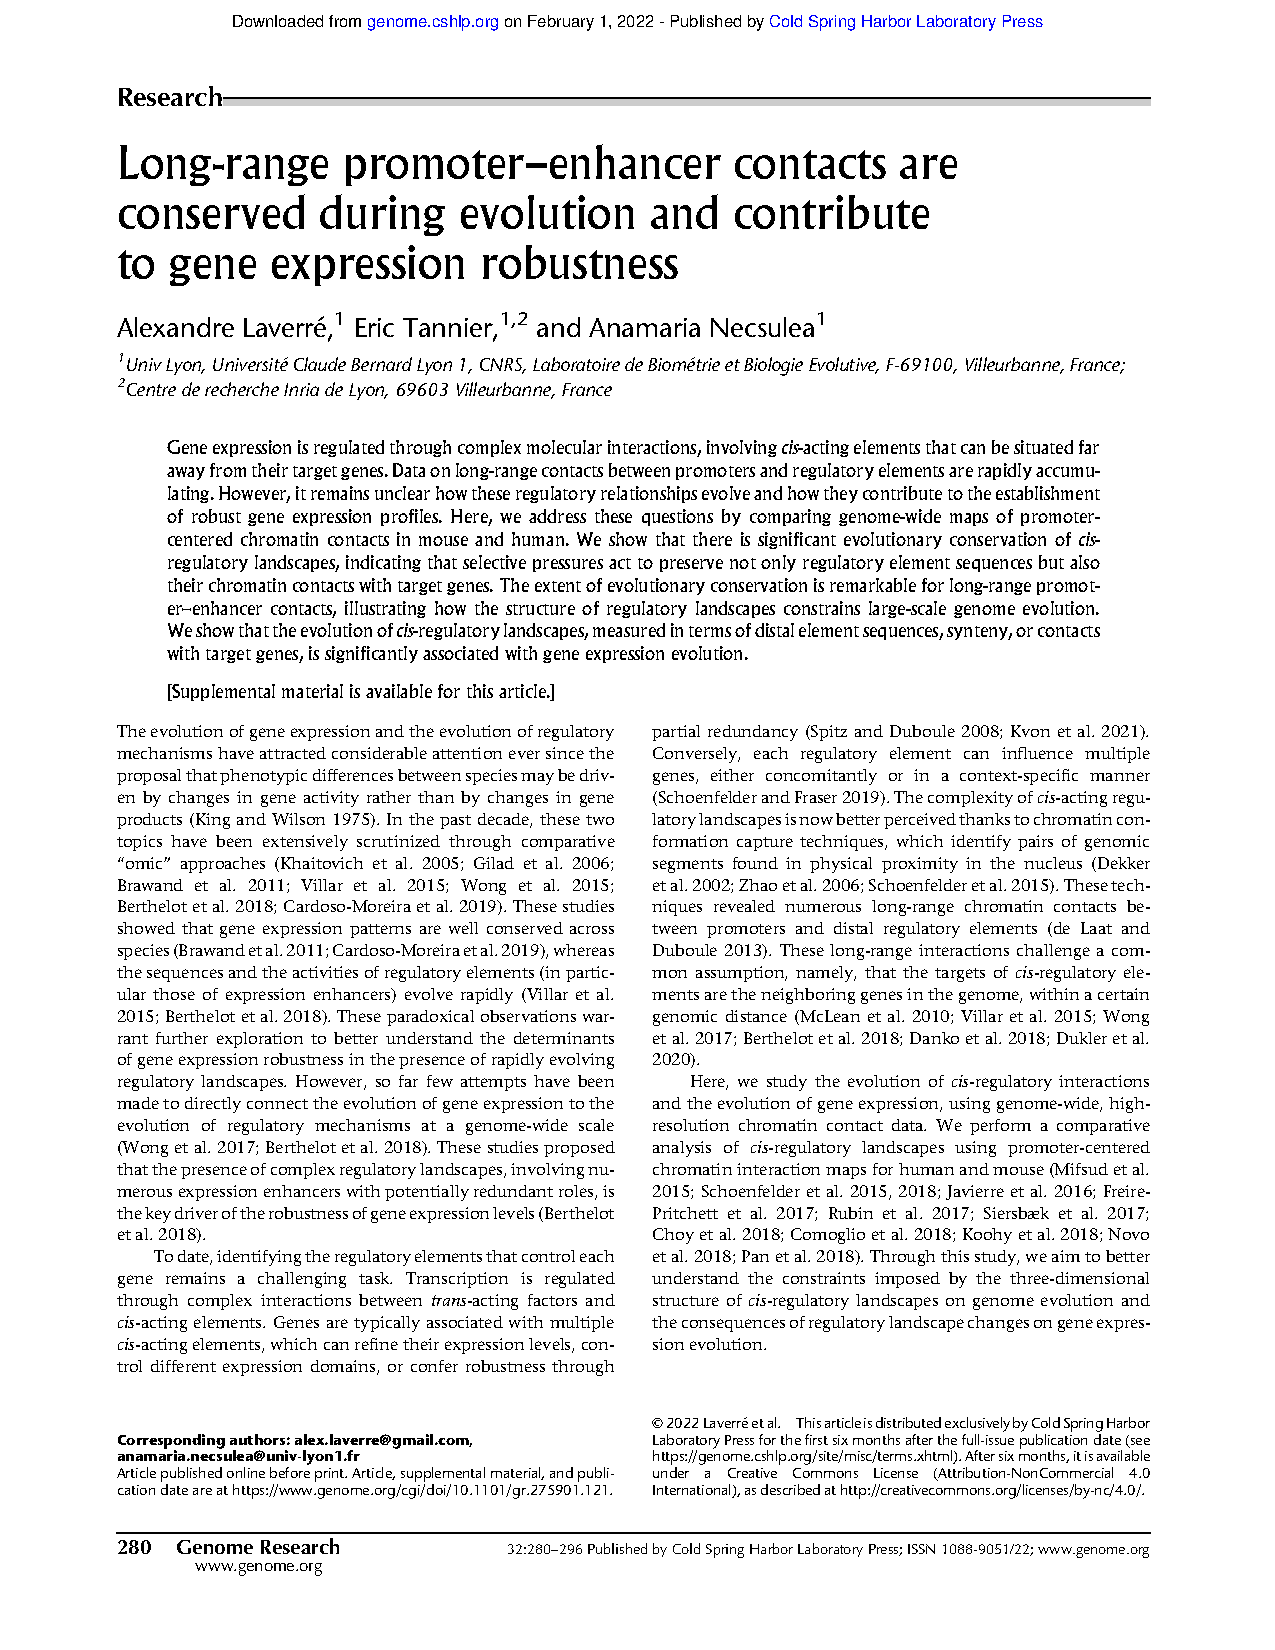
\includepdf[pages=-]{parts/11_Laverre2022.pdf}
    
    \part{Convergence de l’évolution du paysage cis-régulateur et du développement du phallus chez les oiseaux}
    \label{part:chap4}
    \chapter{De l’évolution des paysages cis-régulateurs à l’évolution phénotypique : étude de la perte convergente du phallus chez les oiseaux}
{\hypersetup{linkcolor=GREYDARK}\minitoc}
\label{chap:4-evolpheno}

\section{Introduction}

Les adaptations morphologiques se mettent généralement en place durant le développement embryonnaire des individus et font intervenir des gènes contrôlant la différenciation cellulaire, la croissance et la régionalisation des différentes parties du corps. Ces gènes sont souvent impliqués dans de nombreux processus biologiques et sont alors hautement pléiotropiques ce qui contraint l’évolution de leur séquence codante. Des mutations de la protéine de ces gènes ont souvent de larges conséquences et sont donc délétères pour l’organisme. Il est ainsi théoriquement attendu que la part des mutations codantes par rapport aux mutations non-codantes soit bien plus faibles pour expliquer des changements morphologiques majeurs impliquants de tels gènes pléiotropes (réf). Des variations temporelles ou spatiales de l’expression des gènes seraient en mesure d’expliquer une part importante des changements évolutifs de la morphologie. Par exemple, de nombreuses populations isolées d’épinoches présentent une réduction convergente de la ceinture pelvienne (Shapiro et al. 2004). Ce phénotype est principalement déterminé par l’expression du facteur de transcription Pitx1, qui est impliqué dans le développement de nombreuses structures chez les vertébrés et est sous forte sélection purifiante. Les variations morphologiques observées chez les épinoches seraient ainsi le résultat de nombreuses mutations dans des éléments cis-régulateur de Pitx1 spécifiquement actifs dans ce tissu (Chan et al. 2010; Thompson et al., 2018). L’évolution des paysages cis-régulateurs des gènes peut ainsi participer à des changements morphologiques importants. Les approches de génomique comparative combinées avec des annotations fonctionnelles permettent alors d’identifier les déterminants génétiques qui sont associés à l’évolution d’un phénotype. Détecter la présence, l’absence, l’activité et mesurer le taux d’évolution des éléments cis-régulateurs peut ainsi permettre d’identifier les mécanismes responsables de changement d’expression des gènes à l’origine des variations phénotypiques. \\

Les pertes phénotypiques sont intéressante de ce point de vue car quelque soit la mutation initiale ayant provoqué ce changement, il est attendu d’observer un relâchement des pressions de sélection purifiante sur les séquences impliquées dans le développement et le maintien de ces caractères (Hiller et al., 2013; Roscito et al. 2018). Si ces séquences ne sont pas pléiotropes, elles deviennent non-fonctionnelles et évoluent alors de façon neutre. La présence d’une accumulation de mutations ou plus généralement du changement de taux d’évolution sur une séquence fournissent ainsi des indices sur son rôle dans un changement phénotypique. Les cas de convergence évolutive, dans lesquels plusieurs lignées évoluent indépendamment vers des traits similaires, permettent d’étudier la répétabilité d’un tel processus évolutif (Sackton & Clark, 2019). Les lignées ayant perdu de manière convergente un trait phénotypique présentent ainsi une augmentation parallèle de la divergence sur les séquences impliquées dans ce trait par rapport à leur état ancestral. En analysant les taux d’évolution des gènes codants chez les mammifères, il a par exemple été montré que plusieurs gènes olfactifs présentent une accélération significative spécifique chez les espèces marines où les sens du goût et de l’odorat sont fortement réduits (Chikina et al. 2016). En cherchant à comprendre les mécanismes moléculaires à l’origine de la perte convergente du vol chez les oiseaux, Sackton et collaborateurs n’ont quant à eux pas observé de taux d'évolution convergent dans les séquences codantes (Sackton et al. 2019). Cependant, ils ont détecté des accélérations convergentes des séquences de nombreux éléments cis-régulateurs potentiels présentant des marques de chromatine ouvertes lors du développement des membres antérieurs. Grâce à des alignements de génomes complets, il est ainsi possible d’effectuer des comparaisons des taux d’évolution à l’échelle génomique et ainsi de cibler des régions présentant des patrons d’évolution convergents en tenant compte des relations phylogénétiques entre espèces (Hiller et al. 2013; Prudent et al. 2016; Partha et al., 2019). Par exemple, en se concentrant sur les séquences non-codantes conservées à l’échelle de 24 espèces de vertébrés, plusieurs milliers de régions ont montré des taux d’évolution accélérés convergents chez les 4 espèces considérées ayant un mode de vie souterrain (Roscito et al., 2018). Plusieurs d’entre elles sont situées dans les promoteurs ou proches des gènes liés au développement ou ayant des fonctions relatives aux yeux, ce qui est cohérent avec la forte régression de cet organe chez ces espèces. \\

\begin{figure}[h]
    \centering
    \includegraphics[width=0.8\textwidth, page=1] {figures/chap2/chap4-fig1.png}
    \caption[Approches d'association entre gène et élément \textit{cis}-régulateur par voisinage.]{
    \textbf{Approches d'association entre gène et élément \textit{cis}-régulateur par voisinage.}\\
    }
    \label{fig:chap4-fig1}
\end{figure} 

Finalement, il est possible d’identifier si des pressions de sélection partagées ont produit des phénotypes similaires à partir de bases moléculaires identiques, faisant intervenir des mutations similaires sur les mêmes gènes ou éléments régulateurs. Par exemple, peu de séquences présentent une accélération du taux d’évolution convergent entre les serpents et deux espèces de lézards ayant perdu leurs membres (Figure X; Roscito et al., 2022). La divergence d’éléments cis-régulateurs distincts auraient impacté les patrons d’expression de gènes impliqués à plusieurs étapes dans la voie de signalisation du développement des membres. La potentielle pléiotropie des éléments cis-régulateurs de ces gènes du développement pourraient maintenir une sélection purifiante suffisante sur leurs séquences pour ne pas observer de lien avec la perte phénotypique. De plus, les deux espèces de lézards semblent avoir perdu leurs membres relativement récemment par rapport aux serpents ce qui pourrait ne pas avoir laissé suffisamment de temps pour observer une divergence de l’ensemble des séquences impliqués dans ce phénotype. 

\section{Etude de la perte convergente du phallus chez les oiseaux}
\label{sec:evol-phallus}

Au cours de ma thèse je me suis intéressé à l’évolution convergente du développement du phallus chez les oiseaux. Cet organe est présent chez l’ancêtre des amniotes mais a été réduit ou perdu dans plusieurs lignées d’oiseaux ainsi que chez une espèce de lézard, le tuatara (Brennan et al. 2008; Sanger et al., 2015). Chez les oiseaux, au moins cinq événements indépendants de réduction se seraient produits, notamment dans la lignée des Neoaves représentant plus de 97\% de la diversité actuelle (Brennan et al. 2008). Plusieurs hypothèses évolutives non-exclusives ont été avancées pour expliquer ce changement morphologique majeur (Briskie & Montgomerie 1997). Une première, propose que cette perte soit la conséquence d’une sélection sexuelle pour le choix du partenaire mâle. En effet, l’accouplement chez les espèces d’oiseaux ne possédant pas de phallus nécessite une importante coopération de la femelle pour faire interagir les cloaques des deux individus. Le cloaque est l’orifice postérieur qui est chez ces espèces la seule ouverture commune pour les voies reproductives, digestives et urinaires. La seconde hypothèse avance ainsi que la perte du phallus pourrait être lié à une sélection naturelle pour réduire les risques de transmission sexuelle de pathogène qui pourrait être plus élevés lors d’une intromission (Briskie & Montgomerie 1997). Ce mode de reproduction sans phallus permet également une copulation rapide qui pourrait avoir été sélectionnée pour réduire les risques de prédation (Wesotowski 1999). Les processus développementaux de ce changement phénotypique sont encore mal connus. Chez le poulet, espèce dont les mâles ne possèdent pas de phallus, il a été montré que le tubercule génital (TG) se développe d’une manière similaire au canard à des stades embryonnaires précoces (Herrera et al. 2013). A un stade plus avancé, là où le TG chez le canard continue de se développer pour former un phallus, la croissance du TG chez le poulet s’arrête avant de subir une mort cellulaire. Ce processus pourrait être la conséquence de changement de patron d’expression de plusieurs gènes et notamment de Bmp4 qui activerait l’apoptose du TG chez le poulet (Herrera et al. 2013). Seule l’expression d’une poignée de gène a été analysée en relation avec ce phénotype chez les oiseaux et souvent uniquement de manière qualitative à l’aide d’hybridation in situ sans être quantifié au sein de plusieurs espèces. \\ 

Dans un premier temps, nous avons ainsi étudié les variations des patrons de l’expression de l’ensemble des gènes codants orthologues entre le poulet et le canard au sein de plusieurs stades de développement cruciaux pour la formation du phallus. Pour ce faire nous avons collaboré avec Patrick Tschopp et Maëva Luxey du laboratoire d’évolution de la régulation de l’Université de Bâle en Suisse. Ces derniers ont pu générer des données de transcriptomiques (RNA-seq) qui nous ont permis d’identifier des gènes différentiellement exprimés entre les stades et les espèces. Deuxièmement, afin d’identifier les déterminants des variations de l’expression des gènes, nos collaborateurs ont également produit des données d’épigénomiques (ATAC-seq) indiquant l’accessibilité de la chromatine dans ces mêmes tissus et donc les potentiels éléments cis-régulateurs. Nous avons analysé la présence et la divergence des séquences de ces éléments entre le canard et le poulet mais aussi la conservation de leur accessibilité entre les tissus. Finalement, nous avons analysé les taux d’évolution de ces éléments au sein de plusieurs lignées d’oiseaux dans le but d’évaluer leur corrélation avec la présence ou l’absence du phallus. Nous avons pour celà bénéficié des alignements de génomes complets publiés récemment par le consortium Birds 10K (Feng et al., 2020). Afin d’associer les éléments non-codants candidats avec leur gènes cibles, l’objectif initial était d’utiliser des données de conformation de la chromatine (Hi-C) disponible pour plusieurs échantillons chez le poulet. Cependant pour des contraintes de temps, nous avons pour l’instant utilisé une approche classique de voisinage. \\

L’ensemble de ce travail n’est pas encore complètement finalisé, la partie qui suit n’est ainsi que l’ébauche d’un article à partir des résultats que nous commençons à comprendre. Par la suite, nous avons prévu d’évaluer l’implication de l’évolution des séquences codantes dans l’évolution de ce phénotype. Notamment, nous souhaitons analyser l’évolution du répertoire des gènes ainsi que la divergence des séquences protéiques au sein des génomes d’oiseaux étudiés pour potentiellement détecter des traces d’accélération du taux d’évolution ou de sélection positive. Grâce à PELICAN, un outil développé par des collègues au LBBE, nous avons également prévu d’analyser la convergence des profils d’acides aminés sur les séquences protéiques.\\

Finalement, dans le cadre de ce projet nous avons également séquencé et assemblé le premier génome du hocco à pierre (Pauxi pauxi). Il s’agit d’un oiseau de la famille des Cracidés possédant un phallus et ayant une position phylogénétique intéressante pour l’étude de l’évolution de ce phénotype. Nous avons inclus cet oiseau dans les analyses présentées dans l’article suivant mais nous avons souhaité détailler les caractéristiques de son génome, notamment grâce à des annotations en gènes et en éléments répétés, dans une ébauche d’article située en Annexe \ref{annexe:hocco}.

\section{Article 3 - IPLOSS}
\label{IPLOSS}
    \chapter{Article 3 - Evolutionary mechanisms driving the loss of the intromittent phallus in avian lineages}
\label{IPLOSS}

\begin{center}
    \large Alexandre Laverré$^{\text{1}}$, Maëva Luxey$^{\text{1}}$, Patrick Tschopp$^{\text{2}}$, Anamaria Necsulea$^{\text{1}}$\\
    \vspace{0.5cm}
    \normalsize
    $^{\text{1}}$Univ Lyon, Université Claude Bernard Lyon 1, CNRS, Laboratoire de Biométrie et Biologie Evolutive, F-69100, Villeurbanne, France.\\
    $^{\text{2}}$Laboratory of Regulatory Evolution, DUW Zoology, University of Basel, Basel CH-4051, Switzerland\\
\end{center}

{\hypersetup{linkcolor=GREYDARK}\minitoc}

\section{Abstract}

\section{Introduction}

The vertebrates’ transition from aquatic environments to life on land, more than 300 million years ago, was accompanied by multiple morphological and physiological adaptations, among which internal egg fertilization represented an important reproductive advantage. This mode of reproduction is evidently facilitated by the presence of an intromittent phallus (IP), which helps sperm delivery to the egg. However, although an intromittent male reproductive organ was likely present in the amniote ancestor, it was reduced or entirely lost in multiple avian lineages (Herrera et al. 2013). The evolutionary processes that led to phallus reduction or loss in these species, which nevertheless retained internal fertilization are still unclear. Given that mating with males lacking an IP requires female cooperation and thus allows females more control over fertilization, one hypothesis posits that this process occurred as a result of sexual selection through female choice of mates (Briskie & Montgomerie, 1997). It was also proposed that IP loss was a consequence of natural selection, as it reduced the risk of sexually transmitted diseases, which is elevated in species with a common passage for the urogenital and gastrointestinal systems (Briskie & Montgomerie, 1997). The developmental processes and molecular mechanisms that are responsible for phallus reduction or loss are also not fully understood. It was shown that, in the chicken, this process occurs through an activation of cell death  signals  in  the  developing  genitals,  caused  by  a  gain  of  expression  in  an  important  developmental  factor (Herrera et al., 2013). The genetic basis of this evolutionary change in gene expression is yet unknown. The molecular underpinnings of this morphological transformation are further complicated by the fact that the genes involved in IP development are highly pleiotropic, functioning for example in limb development (ref?). Moreover, many of the regulatory elements that control developmental gene expression are shared between limbs and genitalia (ref). A non-adaptive mechanism for IP reduction/loss can thus be envisaged, as a side-effect of evolutionary changes in other anatomical structures with shared developmental mechanisms (ref).\\

The main aim of this study is to understand the evolutionary processes and molecular mechanisms that drive the loss of the intromittent phallus in avian lineages. The recent publication of numerous avian genome sequences (6), as well as the increasing accessibility of technologies that assay gene expression and regulation, offers an opportunity to address these questions at an unprecedented scale. Through comparative analyses, we propose to evaluate selective pressures associated with IP loss in avian lineages at a genome-wide level, thus revealing the developmental genes and regulatory elements involved in this major morphological transformation. We assessed selective pressures acting at two different genomic levels. \\

- gene expression evolution between chicken and duck
- regulatory sequence activity and evolution between samples
- sequence evolution in birds lineages

We tested the presence  of  selection  on  non-coding  regulatory  elements,  expected  if  changes  in  gene  expression  patterns  (rather than in gene products) are at the origin of the loss of the IP. The existence of multiple independent events of IP reduction/loss during avian evolution, which highlights the remarkable selective pressures that act on this organ, is a key point in our proposal. Our comparative analyses can predict genes and regulatory elements that have exclusive roles in IP development in the avian ancestor, as these elements are expected to evolve rapidly in all IP-lacking lineages, following the loss of functional constraints. \\

\section{Results}

\subsection{Gene expression differences during the development of phallus precursors in chicken and duck}

\begin{figure}[h]
    \centering
    \includegraphics[width=1\textwidth, page=1] {figures/IPLOSS/fig1.png}
    \caption[Gene expression differences.]{
    \textbf{Gene expression differences.}\\
    }
    \label{fig:IPLOSS-fig1}
\end{figure} 

\begin{figure}[h]
    \centering
    \includegraphics[width=1\textwidth, page=1] {figures/IPLOSS/fig2.png}
    \caption[Clusters of temporal gene expression.]{
    \textbf{Clusters of temporal gene expression.}\\
    }
    \label{fig:IPLOSS-fig2}
\end{figure} 


\subsection{Regulatory sequences that control phallus development in chicken and duck}

To determine the regulatory elements that control gene expression during chicken and duck external genitalia development, we analyzed open chromatin regions with the ATAC-seq technique at embryonic stages 29 and 33 (ref). At stage 29, the GT grows in both species, whereas at stage 33 the chicken GT begins to degenerate (ref). In order to identify GT-specific regulatory regions we analysed previously published ATAC-seq data for several organs in both species (ref). The number of open chromatin regions (ATAC-peak) is heterogeneous between samples (Figure 2.A). Chicken GT samples show a surprisingly low number of ATAC-peaks (35,725 and 38,394 for GT 29 and 33) compared to other samples. The number of non-GT duck ATAC-peaks are about two fold higher than other samples (test, pval). \\

- transcription factors binding site enrichment GT vs other (Methods)

The proportions of exonic, intronic and intergenic regions are not significantly different between samples. The number of ATAC-peaks detected in samples are correlated to the sequencing depth (Supplementary Figure, correl test, pval). In order to compare the open chromatin regions between samples without this evident bias, we drew the same number of ATAC-peaks for each sample within species (Methods). We identified ATAC-peaks homologous regions between species from a whole-genome alignment (Methods). The proportion of homologous regions identified did not differ between samples (Supplementary Fig). However, the average identity score is significantly lower for chicken GT ATAC-peaks at stage 29 (Figure 2.B). For each homologous region we determined whether it also covered an ATAC-peak of the other species (Methods). Based on these homologous activities, the factorial correspondence analysis separates the samples by species (Figure 2.C). The chicken GT ATAC-peaks are closest to those obtained in cells of lower and upper limb development. This appears to be consistent with the large number of cis-regulatory regions shared during the development of these organs during development in mouse (ref). Duck genital tubercle ATAC-peaks are most similar to those of the chicken. More than 20\% of the duck GT ATAC-peaks are also active in the chicken GT (Figure 2.D). Less than 15\% of the duck non-GT ATAC-peaks are observed in any of the chicken samples.

\begin{figure}[h]
    \centering
    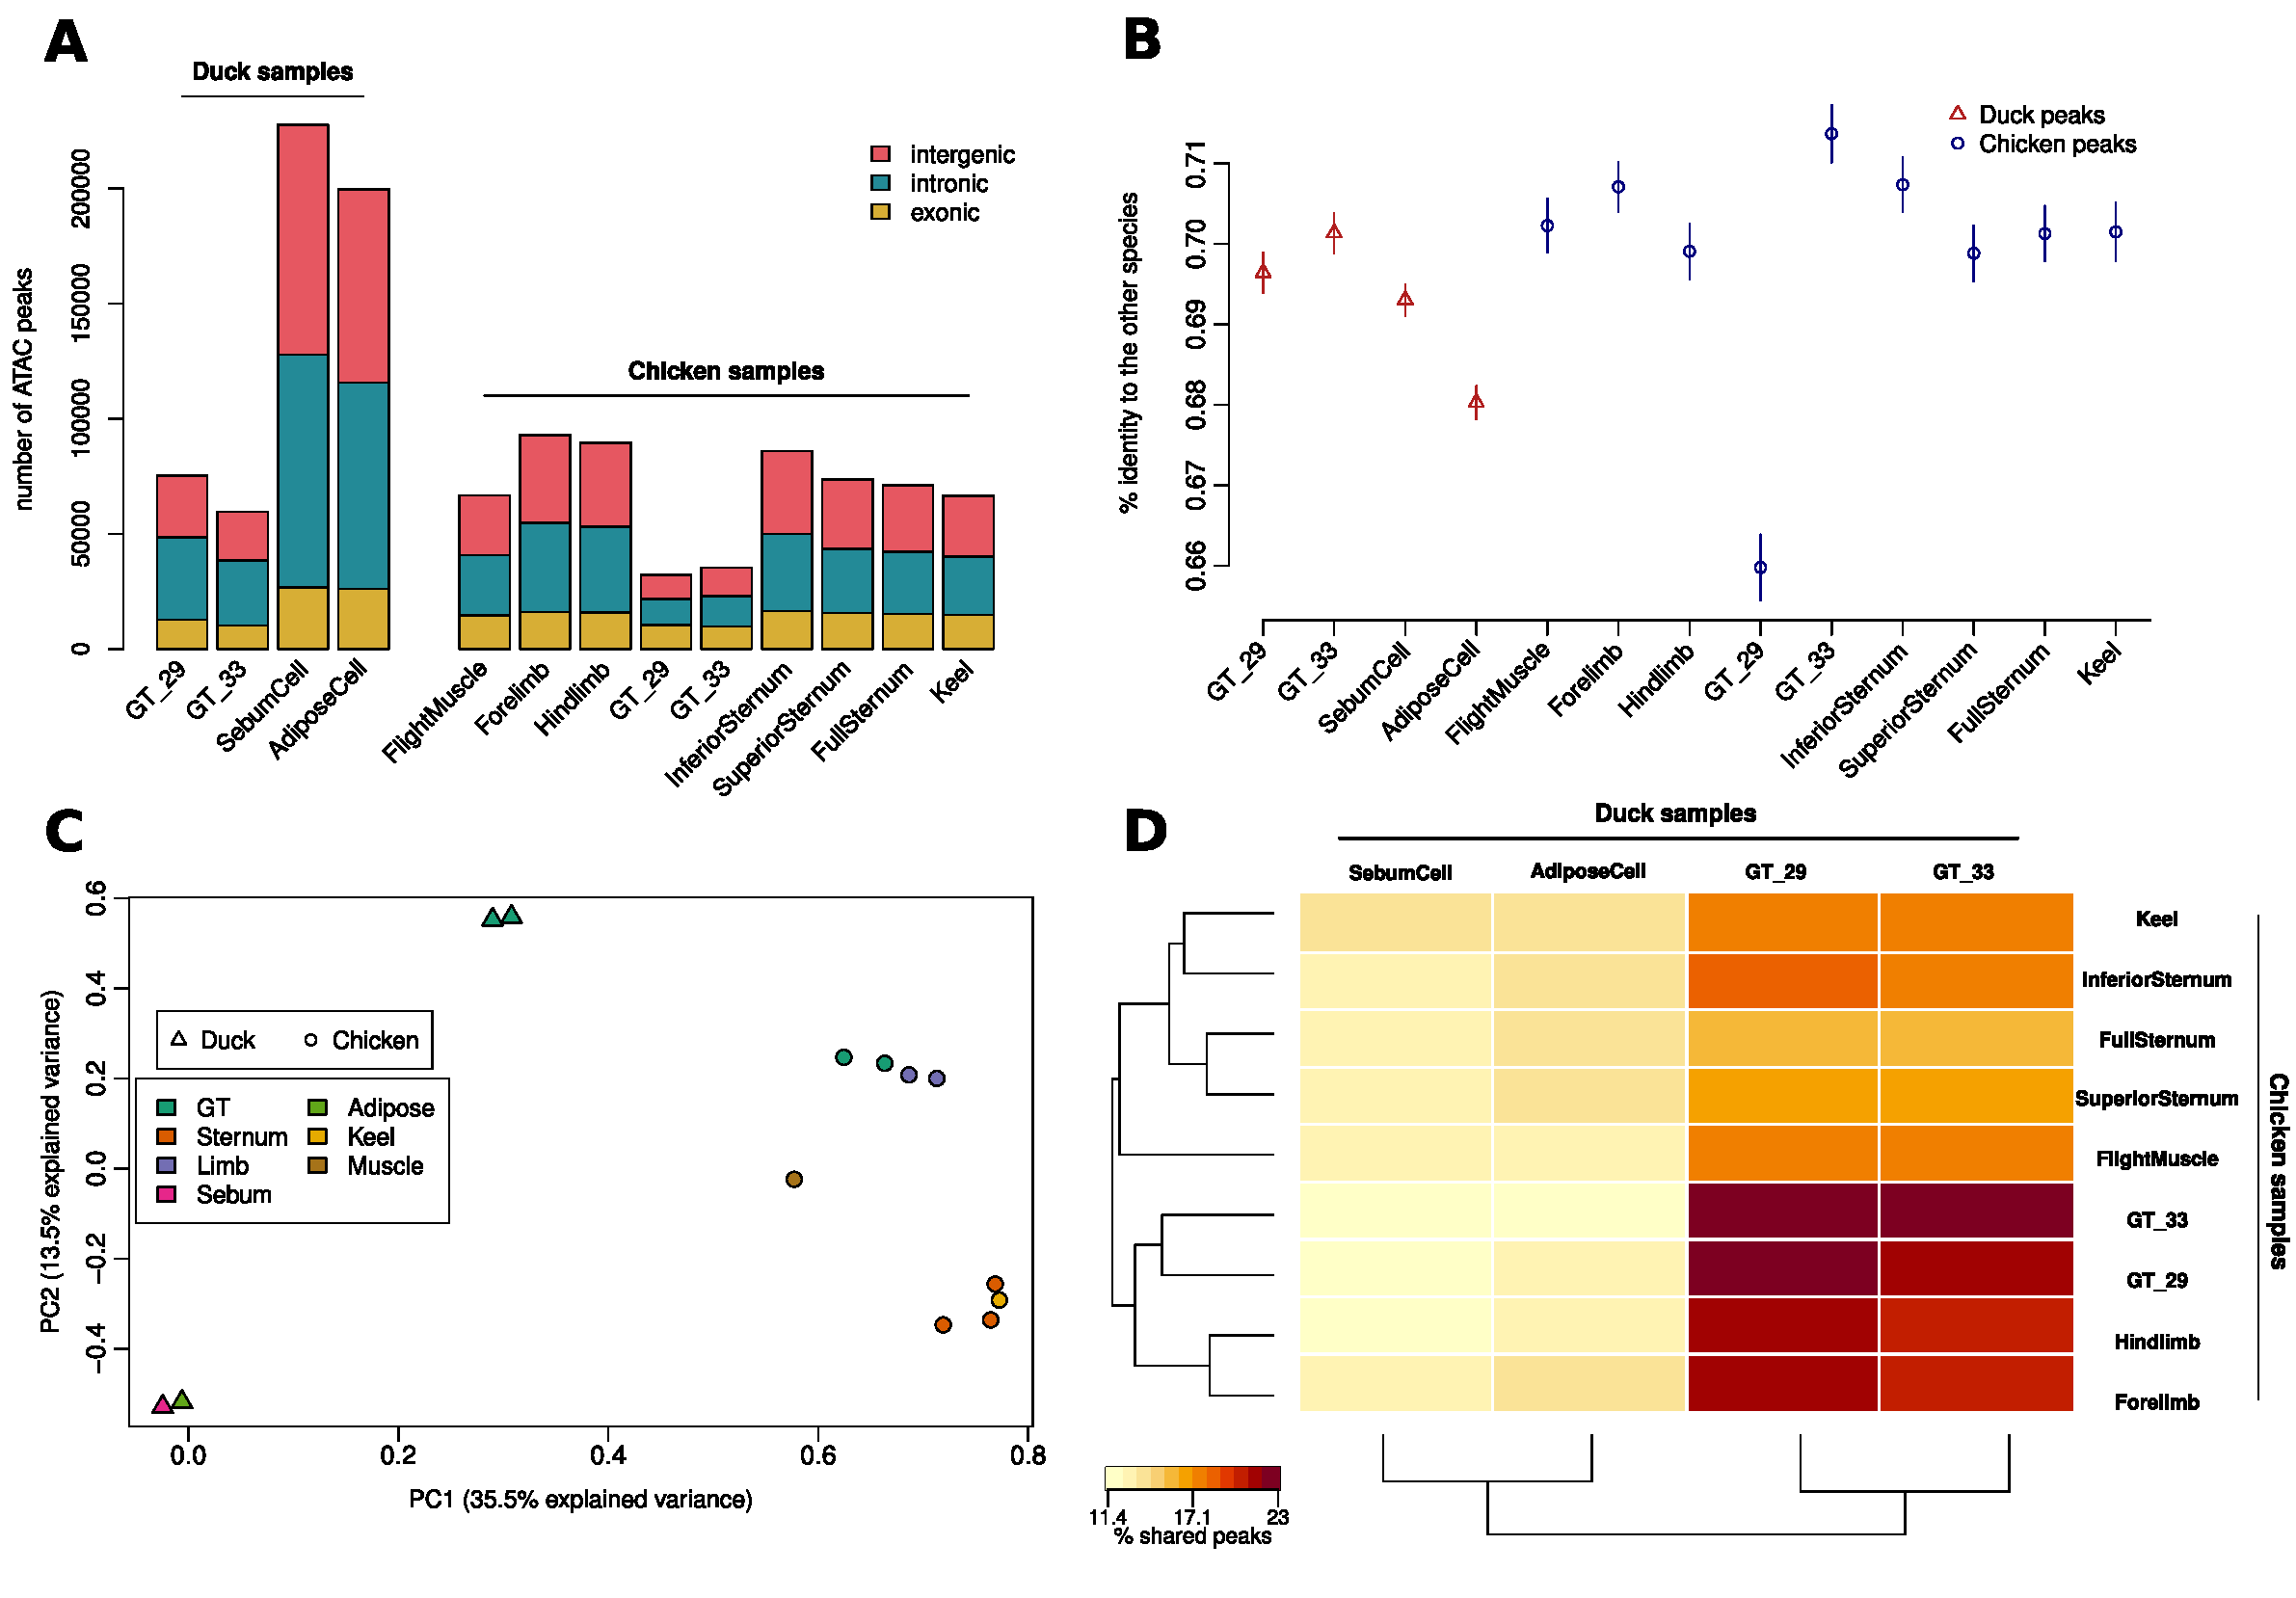
\includegraphics[width=1\textwidth, page=1] {figures/IPLOSS/Fig_peaks.pdf}
    \caption[Comparison of ATAC data in duck and chicken samples.]{
    \textbf{Comparison of ATAC data in duck and chicken samples.}
    \textbf{A.} Distribution of the number of ATAC peaks detected in duck and chicken samples. Peaks are classified according to their overlap with at least one exonic base (exonic, yellow), one non-exonic base (intronic, blue) or no genic base (intergenic, red). 
    \textbf{B.} Distribution of the median percentage identity between sub-sampled duck ATAC peaks sequences (N=63,250) aligned in the chicken genome (red triangle), and between sub-sampled chicken ATAC peaks sequences (N=35,725) aligned in the duck genome (blue circle). Error bars represent the 95\% confidence interval of median. 
    \textbf{C.} Principal component analysis of chicken and duck samples based on homologous subsampled peak activity. Homologous sequences of peaks from a reference species are active in the target species if they overlap at least one base of an ATAC peak in this species (Methods). \textbf{D.} Proportion of subsampled duck ATAC peaks whose homologous sequence overlaps with an ATAC peak in the chicken samples. Dendrograms are produced from the ATAC peak activity binary matrix of each species.  \\
    }
    \label{fig:IPLOSS-fig3}
\end{figure} 

\subsection{Regulatory sequences evolution in bird lineages}
Regulatory elements that control gene expression in the intromittent phallus (IP) are expected to display accelerated evolution in the lineages where this organ was lost, due to relaxation of purifying selection. Evolutionary sequence analyses can thus help identify elements that function in this organ. We analysed the sequence evolution of all non-exonic ATAC peaks detected in duck (N=X) and chicken (N=Y) samples within the aligned genomes of 53 bird species (Figure 3.A; Methods). Of these species, 21 possess an IP and the phylogenetic distribution of this phenotype would represent 5 independent convergent losses (ref). We also complemented this analysis with the identification of non-coding sequences from another duck species (Cairina moschata) conserved in all birds with an IP (Methods). \\

For each aligned sequence, we estimated relative evolutionary rates within each lineage (Methods). A high relative evolution rate in a lineage indicates an accelerated divergence of the sequence relatively to all analysed sequences in that lineage. For each alignment, we estimated the correlation between the relative evolutionary rates and the phenotypic distribution of the IP along the phylogeny (Figure 3.B; Methods). A positive correlation coefficient indicates that the sequence underwent a convergent acceleration of its evolutionary rate in species that lost IP. Conversely, a negative correlation coefficient indicates that lower relative rates of evolution are associated with species that have an IP. The most correlated duck ATAC peak has a median relative evolutionary rate of X in species with IP and Y in species without (Rho = ; FDR=). The proportion of sequences significantly associated with the presence of IP is low for all samples (Figure 3.C; median Duck samples = Y; Supplementary Figure Chicken & Cairina). For duck ATAC peaks, there is a convergently accelerated sequence enrichment in species without IP (test; pval). There is also a higher proportion of sequence correlated with IP evolution in GT samples than in other tissues (test; pval). To assess the impact of the distribution of IP along phylogeny on the correlation with relative evolutionary rates, we performed random permutations of the presence of IP across lineages (Figure 3.D). The median of the observed absolute correlation coefficients is significantly higher than the random permutations (pval=Z). Furthermore, the average number of ATAC peaks correlated with the presence of IP in the random permutations is significantly lower than that observed for the distribution of true phenotypes (obs=1300; random perm.=Y; pval=Z; Supplementary Figure). We detected 535f sequences significantly correlated with the IP evolution and detected by ATAC-seq in duck GT samples. A small proportion of them overlap the chicken ATAC peaks and the conserved Cairina sequences among IP birds (Figure 3.E).

\begin{figure}[h]
    \centering
    \includegraphics[width=1\textwidth, page=1] {figures/IPLOSS/Fig_evol_peaks.pdf}
    \caption[Enrichment for convergently accelerated sequences in birds that lost the intromittent phallus.]{
    \textbf{Enrichment for convergently accelerated sequences in birds that lost the intromittent phallus.}
    \textbf{A.}Species tree. Species names are coloured according to the presence (red) or absence (blue) of an intromittent phallus (IP). The Order to which the species belong is indicated. Obtained from the tree of Feng et al. 2020. 
    \textbf{B.} Example of the relative evolution rate distribution of each species obtained by RERconverge for the sequence from duck ATAC data that is the most correlated with the presence of the phallus (ref RER). Species with IP are associated with lower relative evolution rates than species without IP for this sequence. (R2=X; FDR=Y). 
    \textbf{C.} Proportion of sequences significantly correlated with the presence of IP among ATAC data from duck samples. A greater proportion of these sequences show a higher relative evolution rate in species without IP (blue) than in species with IP (red) within all samples (test; pval). The proportions of correlated sequences are significantly greater in the GT samples than in others (test; pval). 
    \textbf{D.} Distribution of the median correlation coefficients between the relative evolution rate of sequences from duck ATAC data and the presence of the phallus based on 1000 random permutations of the phenotype in the phylogeny. The observed value for the actual phenotype distribution (A.) is shown in red. 
    \textbf{E.} Overlap of homologous sequences correlated with the presence of IP depending on whether they are from duck ATAC data (red), chicken ATAC data (blue) or Cairinia moschata sequences conserved in species with PI (yellow).    \\
    }
    \label{fig:IPLOSS-fig4}
\end{figure} 

\subsection{Inference of regulatory function}

\begin{figure}[h]
    \centering
    \includegraphics[width=1\textwidth, page=1] {figures/IPLOSS/Fig_enrich.png}
    \caption[Detection of genes associated with convergently accelerated sequences in no-IP species.]{
    \textbf{Detection of genes associated with convergently accelerated sequences in no-IP species.}
     \textbf{A.}  Enrichment of convergently accelerated sequences in the vicinity of genes. Each point is a gene represented by the total number of sequences and the number of accelerated sequences in its neighborhood. Colored points are genes with excess convergently accelerated sequences based on a permutation test (5\% FDR). Only genes associated with at least one accelerated sequence are plotted. 
     \textbf{B.} Ontological enrichment of genes associated with convergently accelerated sequences from duck ATAC data. Only the 25 most enriched terms are shown ordered by FDR value.
    \\
    }
    \label{fig:IPLOSS-fig5}
\end{figure} 

\section{Discussion}

\section{Methods}
    
    \part{Discussion}
    \label{part:discussion}
    \chapter{Discussion}
{\hypersetup{linkcolor=GREYDARK}\minitoc}
\label{chap:discussion}

\section{Estimation des paysages \textit{cis}-régulateurs de l’expression des gènes grâce aux contacts de chromatine}

Le premier objectif de ma thèse a été de définir les paysages \gls{cis}-régulateurs de l'expression des gènes à l'aide de données de conformation de la chromatine chez l'humain et la souris. Celles-ci permettent d'associer les gènes à leurs éléments \gls{cis}-régulateurs d'une manière expérimentale qu'il était important de comparer avec les approches communément employées. 

\subsection{Un nouveau regard sur les paysages \textit{cis}-régulateurs}
\subsubsection*{Une mesure expérimentale de l’organisation spatiale du génome}

Les données de contacts de chromatine centrés sur les promoteurs (\acrshort{PCHi-C}) permettent une prédiction expérimentale des paysages \gls{cis}-régulateurs qui est indépendante de l’organisation des gènes. La grande majorité des autres approches d’association entre les gènes et les éléments \gls{cis}-régulateurs se basent sur des inférences strictement computationnelles à partir du voisinage immédiat (en termes de séquence génomique linéaire) autour du promoteur ou du site d’initiation de la transcription du gène. Dans les approches par voisinage que j’ai mentionnées au cours de cette thèse, le domaine de régulation défini pour un gène est directement dépendant de la distance qui le sépare des gènes voisins. La distribution des gènes dans le génome n’étant pas homogène, la densité locale en gènes est alors un facteur déterminant dans la définition des domaines de régulation et donc dans l’attribution des éléments \gls{cis}-régulateurs à leurs gènes cibles. Par exemple, les gènes séparés de leurs plus proches voisins par de grandes distances génomiques se verront attribuer un grand nombre d’éléments \gls{cis}-régulateurs. Avec une telle définition, les frontières des domaines de régulation sont également dépendantes de la qualité des annotations des gènes. En retirant l’annotation d’un gène, la taille des domaines de régulation des gènes avoisinants est artificiellement augmentée, ce qui modifie l’attribution des éléments \gls{cis}-régulateurs aux gènes. Lorsque la distance entre gènes voisins est définie comme la distance entre leurs promoteurs, comme dans GREAT \citep{mclean_great_2010}, la détermination correcte des sites d’initiation de la transcription joue également un rôle. Dans l’outil GREAT par exemple, seuls les gènes possédant une annotation d’ontologie sont utilisés pour définir les domaines de régulation \citep{mclean_great_2010}. Les paysages \gls{cis}-régulateurs sont dans ces cas directement influencés par l'organisation du génome, par la qualité des annotations génomiques et par les critères de sélection des gènes à analyser. \\

Au cours de mes travaux, j’ai pu confirmer que les éléments \gls{cis}-régulateurs qui contactent physiquement les gènes ne sont majoritairement pas ceux qui sont les plus proches sur la séquence d’ADN \citep{smemo_obesity-associated_2014}. De plus, il n’existe qu’une faible concordance entre les deux approches pour ce qui est du nombre d’éléments \gls{cis}-régulateurs attribués aux gènes. Les données de contact de chromatine révèlent des interactions à plusieurs centaines de milliers de paires de bases \citep{laverre_long-range_2022}. Ces relations à grande distance sont pour la majorité exclues \textit{a priori} par des méthodes d’inférence par voisinage. Seuls certains gènes séparés de leurs voisins les plus proches par de très grandes distances intergéniques présentent des associations à longue distance partagées par les deux méthodes (Partie \ref{part:chap2}). A courte distance une plus grande proportion de paires entre gènes et éléments \gls{cis}-régulateurs sont communes. D’autres approches d'inférence des relations régulatrices donnent également beaucoup de poids au voisinage, comme une méthode récente d’association par co-activité des gènes et des \glspl{amplificateur} \citep{hait_ct-focs_2022}. Dans celle-ci, seuls les N \glspl{amplificateur} les plus proches des gènes, où N est un nombre fixé à l'avance, sont considérés pour prédire les relations régulatrices. Celà permet de s’affranchir de la distribution hétérogène des gènes dans le génome mais la structure des paysages \gls{cis}-régulateurs inférés dépend alors de la distribution des amplificateurs.\\

Les données de \acrshort{PCHi-C} ne sont toutefois pas entièrement indépendantes de l’organisation génomique. La taille des régions contactées est dépendante de la distribution des sites de reconnaissance des enzymes de restriction utilisées dans les protocoles de capture de conformation de la chromatine. En effet, la fragmentation du génome au niveau de motifs identiques est nécessaire afin que les régions en proximité physique puissent se liguer deux-à-deux par leurs extrémités. Les sites de fixation de l’enzyme HindIII, employée pour produire les données de \acrshort{PCHi-C} avec lesquelles j’ai travaillé, sont nombreux mais distribués de manière hétérogène dans les génomes de l’humain et de la souris. La taille des régions en contact n’a donc pas de sens biologique et peut être variable. De plus, la taille de ces régions est positivement corrélée avec la probabilité qu'ils recouvrent des promoteurs ou des éléments \gls{cis}-regulateurs. Il est ainsi possible d’obtenir un grand nombre de paires promoteur - \gls{amplificateur} avec un seul contact entre deux régions, sans savoir laquelle ou lesquelles sont biologiquement pertinentes. 

\subsubsection*{Des paysages \textit{cis}-régulateurs cohérents avec les fonctions des gènes}

Pour aller plus loin dans la description des paysages \gls{cis}-régulateurs identifiés par \acrshort{PCHi-C} nous avons developpé GOntact, un outil qui permet d’inférer les fonctions d'un ensemble d'éléments \gls{cis}-régulateurs à partir des annotations fonctionnelles des gènes qu’ils contactent (par exemple celles fournies par Gene Ontology). Le principe de GOntact est similaire à celui de GREAT, qui est couramment utilisé pour annoter les séquences potentiellement \gls{cis}-régulatrices selon les fonctions des gènes voisins et qui a largement fait ses preuves dans de nombreux contextes. En utilisant des éléments \gls{cis}-régulateurs validés expérimentalement et actifs au cours du développement embryonnaire dans le coeur et le cerveau, les enrichissements ontologiques ont révélé des fonctions métaboliques pertinentes avec les deux approches. Malgré les différences d’attribution des éléments à leurs gènes cibles, certaines fonctions sont retrouvées comme enrichies communément par GREAT et par GOntact. D'autres fonctions pertinentes sont détectées uniquement dans l'une des deux approches. La combinaison des méthodes pourraient ainsi apporter des informations complémentaires pour mieux comprendre les rôles des éléments \gls{cis}-régulateurs.

\subsubsection*{Des paysages \textit{cis}-régulateurs cohérents avec l'expression des gènes}
Nous avons confirmé que les contacts de chromatine sont enrichis en relations potentiellement régulatrices \citep{mifsud_mapping_2015, schoenfelder_pluripotent_2015, javierre_lineage-specific_2016}. Les fragments de restriction contactés par les promoteurs des gènes contiennent plus d’amplificateurs, prédits par diverses sources, que la moyenne du génome. Les analyses que j’ai présentées ont également confirmé que les caractéristiques des paysages \gls{cis}-régulateurs déterminés par \acrshort{PCHi-C} sont cohérents avec l’expression des gènes. \\

Premièrement, la complexité des paysages \gls{cis}-régulateurs en terme de nombres d’\glspl{amplificateur} présents dans les régions contactées, est corrélée positivement au niveau d’expression moyen des gènes au sein d’un type cellulaire. Ceci est cohérent avec les modèles de régulation où la fréquence de transcription d’un gène dépend de l’interaction avec plusieurs \glspl{amplificateur} actifs dont l’effet est additif \citep{mifsud_mapping_2015, schoenfelder_pluripotent_2015, javierre_lineage-specific_2016}. Plus ces derniers sont nombreux dans l’environnement physique d’un gène et plus la probabilité d’interaction et donc de transcription est élevée. Il a déjà été montré que les régions contactées par les promoteurs sont enrichies en marques d’histones associés à des \glspl{amplificateur} actifs \citep{javierre_lineage-specific_2016}. La colocalisation des gènes et des éléments \gls{cis}-régulateurs actifs dans des zones du noyau où la transcription est importante pourrait contribuer à cette observation \citep{sutherland_transcription_2009}. Avec une approche de voisinage, en considérant l’ensemble des éléments \gls{cis}-régulateurs répertoriés par le consortium ENCODE, tous tissus et types cellulaires confondus, nous n’avons observé aucune corrélation entre la complexité du paysage et le niveau d’expression (Partie \ref{part:chap2}; \citet{laverre_long-range_2022}). Ceci est contraire à ce qui a été montré en analysant uniquement les éléments éléments \gls{cis}-régulateurs actifs dans le même type cellulaire que celui où on analyse les niveaux d'expression \citep{berthelot_complexity_2018, naville_long-range_2015}. Dans ces études, le nombre d’éléments \gls{cis}-régulateurs actifs dans le voisinage d’un gène est corrélé à son niveau d’expression. Ces résultats suggèrent qu'une part importante de la régulation de l'expression des gènes s'effectue par des éléments \gls{cis}-regulateurs voisins. Ces observations ne sont pas incompatibles, l’entourage physique d’un gène est à la fois composé des éléments voisins sur la séquence mais également d’éléments plus distants rapprochés par des contacts de chromatine. Ceci révèle néanmoins une différence fondamentale entre mes analyses à partir de données combinées de prédictions d’éléments \gls{cis}-régulateurs sur plusieurs \glspl{condition} (tissus, types cellulaires, stades de développement...) et les études à l’échelle d’une seule \gls{condition}. Dans nos définitions de paysage \gls{cis}-régulateur, selon la méthode d’association, les éléments \gls{cis}-régulateurs sont attribués aux gènes sans tenir compte de leur patrons d'activité. Autrement dit, la co-activité entre élément \gls{cis}-régulateur et gène n’est pas prise en compte. Le nombre de relations régulatrices entre gène et \glspl{amplificateur} est donc nécessairement surévalué. Notre objectif était de considérer l’ensemble des éléments \gls{cis}-régulateurs potentiels d’un gène. L’absence de corrélation entre le nombre d’éléments \gls{cis}-régulateurs voisins d’un gène et son niveau d’expression pourrait ainsi indiquer qu’une part importante de ceux-ci ne participe pas à son expression ou du moins qu’ils ne le font pas simultanément dans le même tissu. Pour les paysages \gls{cis}-régulateur mesurés par \acrshort{PCHi-C}, en identifiant les \glspl{amplificateur} actifs, par l’ouverture de la chromatine ou des modifications d’histones par exemple, on pourrait s’attendre a observer une relation avec le niveau d’expression encore plus importante. \\

L’analyse conjointe des données de \acrshort{PCHi-C} et des patrons de l’expression des gènes sur plusieurs échantillons nous a permis de montrer que la complexité des paysages \gls{cis}-régulateurs est positivement corrélée à l’étendue de l’expression des gènes. Plus le nombre d’éléments \gls{cis}-régulateurs contactés par un gène est elevé, plus celui-ci est exprimé dans un grand nombre de \glspl{condition}. Ceci indique qu’indépendamment de l’activité des éléments \gls{cis}-régulateurs, les contacts de chromatine peuvent donner des informations sur le patron d’expression des gènes. Nous avons ainsi confirmé que de nombreux contacts entre un gène et des éléments \gls{cis}-régulateurs sont observés en l’absence d’expression comme le cas du gène \textit{SHH} et de ZRS \citep{schoenfelder_pluripotent_2015}. Ces contacts pré-formés pourraient faciliter l'activation de gènes cruciaux pour l’organisme ou dont l’expression nécessitent une adaptation rapide à des facteurs environnementaux \citep{ing-simmons_independence_2021}. Dès l’activation d’un amplificateur, les gènes qui le contactent pourraient être transcrits sans modification majeure de la structure de la chromatine. La conformation spatiale partiellement pré-formée des génomes permet donc aussi d’inférer des paysages \gls{cis}-régulateurs indépendamment de l’activité des gènes. L’accumulation d’information des contacts de chromatine pourraient ainsi révéler le paysage \gls{cis}-régulateur plus complet d’un gène qui n’est pas nécessairement spécifique d’un type cellulaire. \\

On peut se questionner sur la causalité entre la complexité des paysages \gls{cis}-régulateurs et l’étendue de l’expression des gènes. Il a déjà été montré qu’un gain d’\gls{amplificateur} peut participer à activer l’expression d’un gène dans un nouveau contexte \citep{rebeiz_evolutionary_2011, thompson_novel_2018}. Mais le nombre d’éléments \gls{cis}-régulateurs d’un gène pourrait également augmenter en conséquence de l’étendue ou de la pléiotropie des gènes \citep{monteiro_identifying_2016}. Selon un modèle de Duplication Dégénération et Complémentation, un \gls{amplificateur} \gls{pleiotrope} ancestral pourrait se dupliquer en plusieurs copies qui évolueraient vers une sous-fonctionnalisation. Cette modularité de différents éléments \gls{cis}-régulateurs paralogues pourrait alors affiner la régulation de l’expression des gènes cibles dans plusieurs contextes \citep{murugesan_evolution_2022}. Des analyses comparatives de la fonction et de l’évolution des éléments \gls{cis}-régulateurs sont nécessaires pour mieux comprendre l’origine de la complexité des paysages \gls{cis}-régulateurs et sa relation avec l’évolution de l’étendue d’expression des gènes.

\subsection{Limitations des contacts de chromatine}
\subsubsection*{Des données rares et complexes}
Les données de conformation de la chromatine comme le \acrshort{PCHi-C} sont encore difficilement accessibles. Ces données sont produites grâce à des techniques bio-moléculaires complexes et coûteuses et dont les protocoles peuvent être difficiles à mettre en place. Les sondes génétiques qui permettent de cibler les promoteurs des gènes sont notamment dépendantes du génome considéré et sont actuellement disponibles uniquement pour l’humain et la souris, ce qui complique l’emploi sur des espèces non modèles. Ces sondes spécifiques ne ciblent d’ailleurs pas tous les gènes (70\% des gènes codants pour des protéines chez l’humain), ce qui ne permet donc pas d’étudier l’ensemble des paysages \gls{cis}-régulateurs. La non-homogénéité des protocoles, notamment par l’utilisation d'enzymes de restriction différentes, peut également compliquer les comparaisons entre les études. De plus, le traitement bioinformatique et statistique de ces données demande du temps et d’importantes ressources. Durant ma thèse, j’ai par exemple compilé toutes les données disponibles de \acrshort{PCHi-C} aux protocoles identiques, ce qui représente plus de 4 Téraoctets de lectures de séquençage brutes et, une fois le traitement bio-informatique maîtrisé, plus d’1 mois de traitement sur le serveur de calcul du LBBE. \\

Les méthodes de Hi-C, qui mesurent les contacts de chromatine sur l’ensemble des loci, commencent à s’accumuler et à se populariser notamment pour l’amélioration de l’assemblage de génome \citep{ghurye_integrating_2019}. À l’origine, la résolution de cette technique ne permettait pas d’inférer avec précision les paysages \gls{cis}-régulateurs des gènes. L’augmentation de la profondeur de séquençage et le développement de méthodes statistiques récentes pourraient cependant permettre d’améliorer sa précision et sa sensibilité \citep{lagler_hic-act_2021}. Les nombreuses données publiées de Hi-C pourraient être exploitées pour étudier les paysages \gls{cis}-régulateurs dans un plus grand nombre de tissus et d’espèces. Par exemple, dans l’étude de l’évolution du phallus chez les oiseaux, nous comptons prochainement traiter des données récentes de Hi-C disponibles pour le canard et le poulet pour améliorer les prédictions d’associations entre les gènes et les éléments \gls{cis}-régulateurs \citep{zhu_three_2021, fishman_3d_2019, li_comparative_2022}.

\subsubsection*{Des contacts de chromatine ignorés}
Dans nos études, nous avons analysé uniquement les contacts intra-chromosomiques entre régions promotrices et non-promotrices. Ces interactions en \gls{cis} sont les plus fréquentes et décrivent des relations régulatrices les plus généralement admises. Cependant plus de 10\% des contacts étudiés chez l’humain mettent en interaction deux régions promotrices. Les premières études ayant analysé des données de contact ont montré que ces interactions sont enrichies en gènes fonctionnant dans des voies métaboliques proches. Les gènes mis en contact ont tendance à fixer les mêmes facteurs de transcription ce qui suggère qu'il pourrait s'agir de gènes co-régulés \citep{schoenfelder_pluripotent_2015}. Ces gènes pourraient être co-localisés dans des micro-environnements du noyau pour coordonner la régulation de leur expression \citep{osborne_active_2004}. Ces micro-environnements sont communément appelés des “usines” de transcription. Dans ces “usines”, la concentration en facteurs de transcription, en ARN polymérase active et en molécules associées aux modifications des ARN messagers est plus élevée \citep{sutherland_transcription_2009, rieder_transcription_2012}. Les régions promotrices ciblées pouvant être relativement grandes, il est également probable qu’elles contiennent d’autres éléments \gls{cis}-régulateurs en plus des promoteurs. Ces contacts entre promoteurs pourraient donc agir d’une manière similaire aux contacts régulateurs “classiques”, qui ont lieu entre promoteurs et amplificateurs. De plus, les fonctions des promoteurs et des \glspl{amplificateur} peuvent être très similaires. Ils peuvent par exemple fixer des facteurs de transcription communs. Il a été montré que 2 à 3\% des promoteurs chez l’humain présentent une activité d’\gls{amplificateur} de l’expression de gènes distaux \citep{dao_genome-wide_2017}. Cette observation pourrait venir complexifier la caractérisation des paysages \gls{cis}-régulateurs.\\

Des contacts inter-chromosomiques sont également présents dans les données de \acrshort{PCHi-C}, ils représentent 1,5\% des interactions combinées chez l’humain. De tels contacts ont déjà été observés pour des gènes activement transcrits et révèlent des relations régulatrices fonctionnelles \citep{spilianakis_interchromosomal_2005}. Ces interactions en \gls{trans} questionnent les mécanismes moléculaires à l’origine de l’organisation spatiale des chromosomes dans le noyau et le maintien de ces loci en proximité physique sans boucle de la chromatine classique. Le facteur de transcription CTCF pourrait jouer un rôle d’intermédiaire pour diriger ces régions en proximité physique \citep{ling_ctcf_2006}. Des boucles de chromatine en \gls{cis} de différents chromosomes pourraient également se colocaliser dans les mêmes usines de transcription. Les contacts interchromosomiques observés seraient alors le résultat d’interactions indirectes via les usines de transcription. L’analyse de la co-expression de ces gènes, ainsi que l’observation en microscopie optique de leur localisation dans le noyau pourrait permettre de mieux comprendre ces interactions atypiques.

\subsubsection*{La régulation en absence de boucle promoteur-enhancer}
Bien que le modèle de contact physique entre promoteur et \gls{amplificateur} soit largement supporté par de nombreuses données et études distinctes, plusieurs observations indiquent que les boucles de la chromatine ne sont pas obligatoires pour les interactions régulatrices. Certaines relations essentielles entre \glspl{amplificateur} et promoteurs existent sans contact physique classique apparent \citep{alexander_live-cell_2019}. Par exemple, le gène \textit{Shh} s’éloigne physiquement de plusieurs de ses \glspl{amplificateur} essentiels dans le développement du tube neural chez la souris alors que son expression augmente \citep{benabdallah_decreased_2019}. Plusieurs modèles ont été proposés pour expliquer de telles relations régulatrices, comme le “kiss and run model”, où le contact entre un \gls{amplificateur} et le promoteur d’un gène permet de transférer des facteurs de transcription mais n’a pas besoin d’être maintenu en proximité pour être fonctionnel ou encore le modèle d’un gradient d’activité de facteur de transcription \citep{karr_transcription_2022}. \\

Des études expérimentales ont également montrées qu’en retirant artificiellement les principales molécules responsables de l’organisation tridimensionnelle de la chromatine, comme le facteur de transcription CTCF ou la cohésine, la plupart des gènes continue à être exprimés à des niveaux normaux \citep{schwarzer_two_2017, rao_cohesin_2017}. Dans ces expériences, les domaines d’association topologique (TAD) et la majorité des boucles de chromatine à grande distance sont éliminées. Cette délétion entraîne peu de changement sur les gènes normalement inactifs dans ces échantillons, mais modifie l’expression d’une minorité des gènes déjà exprimés. La condensation de la chromatine et les marques des histones sont conservées et pourraient expliquer cette observation. Ces marques épigénétiques définiraient des compartiments génomiques à fine échelle indépendamment de la conformation tridimensionnelle des chromosomes \citep{schwarzer_two_2017}. Parmi les gènes dont l’expression est modifiée, une plus forte proportion de gènes subissent une diminution qu’une augmentation de l’expression. De plus, les gènes entourés par de grandes régions intergéniques sont les plus impactés par cette diminution \citep{schwarzer_two_2017}. Ceci pourrait donc s’expliquer par la perte de contact avec des éléments \gls{cis}-régulateurs distaux. En l’absence de cohésine, les gènes avec de nombreux éléments \gls{cis}-régulateurs proches voisins ont tendance à être surexprimés par rapport aux gènes qui en ont moins. Une plus forte compartimentalisation du génome en structures plus restreintes est en effet observée dans ces expériences \citep{rao_cohesin_2017}. En l’absence de contact à longue distance, les éléments \gls{cis}-régulateurs pourraient ainsi être redirigés vers les gènes à proximité. Cette réorganisation des paysages \gls{cis}-régulateurs et la possible redondance des séquences \gls{cis}-régulatrices pourraient permettre de temporiser des variations de structure mais pourrait avoir des conséquences plus grandes à large échelle sur le patron d’expression. La caractérisation plus fine des paysages \gls{cis}-régulateurs des gènes à l’aide de données à plus haute résolution comme le \acrshort{PCHi-C} pourrait permettre de mieux comprendre la dynamique des boucles de chromatine. Plus généralement, ces études confirment que d’autres mécanismes que les contacts à grande distance sont à l’oeuvre dans la mise en place des associations spécifiques entre les promoteurs des gènes et les éléments \gls{cis}-régulateurs (cf modèle complet de \citet{schoenfelder_long-range_2019}).

\subsection{Vers une multiplication des approches d’association}
\subsubsection*{Complémentarité des approches de voisinage et de contact dans GOntact}

Les approches de voisinage sont dépendantes de l’organisation génomique pour définir les associations entre gènes et éléments \gls{cis}-régulateurs et sont par définition limitées aux régions proches des gènes. Au contraire, les contacts de chromatine peuvent permettre d’associer des régions à très grandes distances, mais il est délicat de considérer avec une grande fiabilité les interactions à courtes distances. En effet, deux loci proches linéairement sur le génome ont une forte probabilité d’être proche spatialement dans le noyau. On observe ainsi que la distance génomique entre deux loci est corrélée positivement à la distance physique dans le noyau. Les traitements statistiques des contacts de \acrshort{PCHi-C} prennent en compte ce biais pour définir les interactions significatives, mais la proportion de faux positifs reste élevée pour les contacts à courte distance \citep{cairns_chicago_2016}. En éliminant par précaution les contacts à courte distance, la distribution des distances entre gènes et éléments \gls{cis}-régulateurs est différente selon une approche par \acrshort{PCHi-C} et par voisinage. Ces associations sont cependant biologiquement pertinentes au vu des fortes corrélations entre l’expression des gènes et les activités des \glspl{amplificateur} à courte distance \citep{laverre_long-range_2022}. Le modèle de régulation à courte distance très largement utilisé reste donc pertinent dans de nombreux cas. Néanmoins les contacts à grande distance révèlent également des fonctions cohérentes, confirmant certaines associations par voisinage mais en révélant de nouvelles. Ainsi dans GOntact nous proposons une méthode "hybride" d'association entre gène et éléments \gls{cis}-régulateurs pour tirer partie de la présence de relations régulatrices dans le voisinage et à grande distance des promoteurs des gènes. \\

\subsubsection*{Nombreuses méthodes d'inférence de relations régulatrices}

De nombreuses méthodes d’asociation entre gène et éléments \gls{cis}-régulateurs ont été développées que ce soit par voisinage (à la manière de GREAT \citet{mclean_great_2010}), par conformation de la chromatine (\acrshort{PCHi-C}), par conservation évolutive de la synténie entre gènes et éléments \gls{cis}-régulateurs (PEGASUS: \citet{clement_enhancergene_2020}), par co-activité (FOCS : \citet{hait_focs_2018}), par corrélation de l’accessibilité de la chromatine (Cicero: \citet{pliner_cicero_2018}, SnapATAC: \citet{fang_comprehensive_2021}) ou encore par la présence de marques épigénétiques identiques (TargetFinder : \citet{whalen_enhancerpromoter_2016}), pour ne citer que quelques exemples. Chacune permet d’obtenir un aperçu différent de l’organisation des paysages \gls{cis}-régulateurs des gènes tout en comportant des biais techniques ou inhérents aux méthodes. Multiplier les approches et construire une base de données qui intégrerait les prédictions d’éléments \gls{cis}-régulateurs et leurs potentiels gènes cibles au fur et à mesure des publications pourrait permettre de caractériser de manière systématique les paysages \gls{cis}-régulateurs des gènes. De tels outils commencent à émerger par exemple avec GeneHancer \citep{fishilevich_genehancer_2017}. Celui-ci utilise les prédictions d’\glspl{amplificateur} de l’humain provenant de quatre sources différentes ainsi que trois approches distinctes pour l’association entre gènes et amplificateurs. Il intègre notamment les résultats de la première étude de \acrshort{PCHi-C} \citep{mifsud_mapping_2015}. GeneHancer calcule ainsi un score de confiance pour chaque \gls{amplificateur} et pour chaque association avec un gène selon le nombre de sources différentes qui l'identifient. Cette méthode permet d’obtenir un large nombre d’associations mais nécessiterait d’intégrer de nombreuses données supplémentaires pour comprendre les mécanismes de la régulation de l’expression des gènes dans un grand nombre de contextes. L’accumulation de données nécessite de collaborer à l’échelle internationale et de proposer des initiatives communes pour démêler et rendre cohérents les efforts dans la compréhension des génomes.

\section{Corrélation entre l’évolution de l’expression des gènes et des paysages \textit{cis}-régulateurs}

Le second objectif de ma thèse a été d'analyser l'évolution des paysages \gls{cis}-régulateurs chez les vertébrés à partir des contacts de la chromatine  et d'analyser ses relations avec l'évolution de l'expression des gènes à partir de comparaisons entre l'humain et la souris. 

\subsection{Contacts de chromatine conservés entre humain et souris}
Mes travaux ont montré que les contacts de la chromatine centrés sur les promoteurs des gènes sont plus conservés qu’un attendu neutre entre des espèces distantes comme l’humain et la souris. Les régions contactées sont également conservées en séquence et en synténie avec leurs gènes cibles à l'échelle des vertébrés. Des structures homologues séparées par de grandes distances génomiques sont significativement maintenues en contact dans des types cellulaires qui ne sont pas nécessairement les mêmes. De plus, les gènes dont les paysages \gls{cis}-régulateurs sont les plus conservés sont enrichis en gènes dont le patron d’expression est fortement contraint comme les gènes du développement. Cette observation donne un argument supplémentaire à la pertinence fonctionnelle des interactions de la chromatine mesurées à cette échelle. La conservation des contacts de chromatine est également en accord avec ce qui a déjà été observé pour l’évolution des domaines d’associations topologiques (\acrshort{TAD}s), des régions génomiques où les contacts sont favorisés \citep{dixon_topological_2012, harmston_topologically_2017, krefting_evolutionary_2018}. \\

Ceci indique également que d’importantes pressions de sélection contraignent l’évolution à grande échelle de l’organisation génomique. Les réarrangements perturbant ces relations régulatrices sont contre-sélectionnés comme cela a déjà été montré par les analyses de la distribution des points de cassure dans le génome \citep{lemaitre_analysis_2009, swenson_large-scale_2019}. L’importante conservation de la synténie entre les gènes et les éléments \gls{cis}-régulateurs à grande distance corréle effectivement avec l’organisation spatiale du génome \citep{clement_enhancergene_2020}. La prise en compte de l'organisation tridimensionnelle du génome et des paysages \gls{cis}-régulateurs est ainsi importante pour comprendre l’impact des réarrangements sur l'expression des gènes. Les réarrangements entre un gène et un élément \gls{cis}-régulateur n’entraînent en effet pas nécessairement une perturbation du contact \citep{symmons_SHH_2016}. Des promoteurs et amplificateurs séparés pas des distances linéaires très différentes entre deux espèces peuvent-être spatialement proches et ainsi conserver une relation régulatrice homologue \citep{veron_close_2011}. Le maintien des loci dans une certaine gamme de distance est possible, ce qui explique que l’évolution de la distance à l’intérieur des \acrshort{TAD}s suivrait une dynamique évolutive similaire à l’évolution de la taille des introns \citep{clement_enhancergene_2020}. Analyser conjointement les contacts de chromatine et les réarrangements pourraient permettre d’expliquer les mécanismes moléculaires à l’origine de l’évolution de l’expression de certains gènes. 

\subsection{Absence de corrélation avec l’évolution du niveau d’expression des gènes}

Nous n’avons pas observé de corrélation entre l’évolution des paysages \gls{cis}-régulateurs, en terme de séquence, de synténie ou de contact de chromatine, et l’évolution du niveau moyen d’expression dans des types cellulaires comparables entre l’humain et la souris. Ces différences quantitatives sont difficiles à mesurer entre des espèces aussi distantes que l’humain et la souris, d’autant plus que nous avons analysé des données provenant de différentes sources. Les niveaux d’expression (RNA-seq), la prédiction d’éléments \gls{cis}-régulateurs (combinés sur de nombreux échantillons) et les informations de contact (\acrshort{PCHi-C}), proviennent d’études différentes sur des tissus différents et donc comprennent une source importante de biais. \\

Cette observation pourrait également être en accord avec les précédentes études qui ont montré des paysages \gls{cis}-régulateurs évoluant rapidement (par leur séquence et leur activité) \citep{cheng_principles_2014, villar_enhancer_2015}, contrairement aux niveaux d’expression qui évoluent lentement chez les vertébrés \citep{brawand_evolution_2011, cardoso-moreira_gene_2019, berthelot_complexity_2018}. La redondance fonctionnelle des éléments régulateurs pourrait être un mécanisme important pour expliquer cette robustesse d’expression \citep{berthelot_complexity_2018, osterwalder_enhancer_2018, kvon_enhancer_2021}. Au niveau de l’évolution de la séquence, la redondance fonctionnelle permettrait de relâcher les pressions de sélection sur chacun des éléments \gls{cis}-régulateurs. Cette forme de compensation des mutations serait d’autant plus importante que le paysage \gls{cis}-régulateur est complexe. Cette compensation pourrait également s’effectuer à différentes échelles par les nombreux autres mécanismes régulateurs de l’expression. Par exemple, il a été montré que de nombreuses mutations en cis pouvaient être compensées par des variations de la régulation en \gls{trans} \citep{goncalves_extensive_2012, mack_gene_2016}. De plus, la faible spécificité des motifs reconnus par les facteurs de transcription serait en mesure d’assurer la conservation de la fonction régulatrice d’une séquence divergente. Certains éléments \gls{cis}-régulateurs fortement conservés en micro-synténie avec leurs gène cibles à l’échelle des métazoaires semblent par exemple avoir conservé leur fonction tout en ayant suffisamment divergé pour n’être plus alignables entre espèces \citep{wong_deep_2020}. Cette importante dégénérescence du “code de régulation” des éléments \gls{cis}-régulateurs doit être investiguée pour mieux comprendre l’évolution des mécanismes régulateurs de l’expression des gènes. A la manière des séquences codantes, celà permettrait d’identifier des mutations “silencieuses” ou non pour la fonction des éléments \gls{cis}-régulateurs et ainsi potentiellement déceler des changements de forces sélectives. Cela pourrait également permettre d’expliquer l’importante variabilité des conséquences de l’évolution des séquences \gls{cis}-régulatrices. En effet, des cas de perturbation extrême comme une délétion complète d’éléments \gls{cis}-régulateurs fonctionnels sans conséquence phénotypique \citep{osterwalder_enhancer_2018} co-existent avec des cas où de simples mutations ponctuelles engendrent un important changement morphologique ou sont associées à des maladies \citep{corradin_enhancer_2014, kvon_progressive_2016}. 

\subsection{Corrélation avec l’évolution du patron d’expression des gènes}
La différence d’échelle entre la prédiction des paysages \gls{cis}-régulateurs modulables obtenus à partir des données de \acrshort{PCHi-C} et les niveaux d’expression mesuré dans un seul échantillon révèle une nécessité d’observer un tableau plus complet de l’activité des gènes. C’est la raison pour laquelle nous avons analysé les patrons de l’expression des gènes à travers plusieurs organes et stades de développement comparables entre l’humain et la souris \citep{cardoso-moreira_gene_2019}. Les différences mesurées sont donc davantage qualitatives et sont plus à même de révéler des changements majeurs comme des gains ou des pertes d’expression dans une \gls{condition}. \\

Nous avons observé une corrélation entre l’évolution des paysages \gls{cis}-régulateurs et l’évolution du patron d’expression des gènes. Les \glspl{amplificateur} les plus conservés en séquence, mais également ceux maintenus en synténie avec les gènes ou encore en contact de chromatine conservé entre l’humain et la souris sont associés à des gènes aux patrons d’expression conservés. Cette observation est également en accord avec ce qui avait été observé pour les gènes à l’intérieur des \acrshort{TAD}s conservés à l’échelle des vertébrés qui sont associés à une plus grande conservation de leur patron d’expression entre humain et souris \citep{krefting_evolutionary_2018}. Analyser l’expression des gènes dans un grand nombre de contextes permettrait d’augmenter la probabilité d’observer les variations du paysage \gls{cis}-régulateur qui impactent l’expression des gènes. En effet, de par la compensation des mécanismes mais également de la pré-formation de la structure de la chromatine, le gain ou la perte d’un contact entre un gène et un éléments \gls{cis}-régulateur n’entraine pas nécessairement une modification de son l’expression dans l’ensemble des contextes. 

\subsection{Analyse d’autres catégories de gènes}
Dans ce travail, nous avons seulement considéré les gènes codants pour des protéines. Il serait également intéressant d’inférer les paysages \gls{cis}-régulateurs des gènes non-codants, notamment les loci produisant de longs ARNs non-codants, dont la régulation et les rôles sont encore largement incompris \citep{mercer_long_2009, ransohoff_functions_2018}. Ces gènes peuvent notamment être impliqués dans de nombreux processus de régulation de l’expression d’autres gènes à différentes échelles, pré et post-transcriptionnelles. Ils peuvent agir sur l’expression des gènes en \gls{cis}, par l’action directe dans le voisinage proche ou potentiellement par contact de chromatine à plus longue distance. Les données de \acrshort{PCHi-C} que j’ai analysées devraient permettre d’étudier l'évolution de leurs paysages \gls{cis}-régulateurs entre l’homme et la souris, et peut-être même de prédire leurs gènes cibles, si la régulation se fait par contact de chromatine.\\

De plus, nous avons restreint nos analyses aux gènes qui sont orthologues un-à-un entre les espèces. Nous avons donc exclu deux classes de gènes intéressants : ceux qui ont subi des duplications depuis la divergence des deux espèces, et ceux qui ont été perdus (pseudogénisés) au cours de l’évolution dans l’une des deux lignées. Ces deux catégories de gènes sont intéressantes pour des raisons différentes. D’un côté, l’évolution de l’expression des gènes après duplication a attiré beaucoup d’attention \citep{brunet_gene_2006, guschanski_evolution_2017, carelli_repurposing_2018}. De nombreux cas de changements de patron d’expression entre les copies des gènes après duplication ont été mis en évidence. Les changements des paysages \gls{cis}-régulateurs qui sont associés à ces changements d’expression ne sont pas encore parfaitement compris, et les données de \acrshort{PCHi-C} pourraient aider pour répondre à cette question. De l’autre côté, en ignorant les cas de pseudogénisation nous excluons une potentielle conséquence majeure des changements des paysages \gls{cis}-régulateurs : des cas extrêmes de changement de régulation (tels que ceux entraînés par de grands réarrangements génomiques) pourraient mener à une perte de fonction des gènes et donc à une pseudogénisation. Inversement, une forte divergence de certains éléments \gls{cis}-régulateurs pourrait être expliquée par la perte de fonction des gènes cibles. La prise en compte de ces cas de pseudogénisation permettrait de mieux saisir les implications phénotypiques de l’évolution des mécanismes \gls{cis}-régulateurs.

\section{Relation avec l’évolution phénotypique}

Finalement, mon dernier objectif a été d'investiguer les relations entre l'évolution des paysages \gls{cis}-régulateurs, l'évolution de l'expression des gènes et l'évolution phénotypique. En étudiant la perte convergente du phallus chez plusieurs lignées d’oiseaux, nous souhaitions mieux comprendre les déterminants génétiques de ce changement phénotypique majeur.

\subsection{Patrons d’expression conservés malgré les changements phénotypiques}

Premièrement, en comparant des profils d’expression au cours du développement du tubercule génital nous avons montré que l’expression de la grande majorité des gènes suit une trajectoire temporelle similaire entre le poulet et le canard. Cette observation est en accord avec l’évolution lente de l’expression des gènes observés dans plusieurs études malgré d’importantes variations morphologiques \citep{brawand_evolution_2011, cardoso-moreira_gene_2019}. Le caractère fortement pléiotropique des gènes exprimés au cours du développement est généralement mis en avant pour expliquer ces résultats. Dans le cas du développement du tubercule génital, il est en effet connu que de nombreuses voies de signalisation sont partagées avec le développement des membres chez la souris \citep{lonfat_convergent_2014,infante_shared_2015}. De plus, comme nous l’avons vu tout au long de cette thèse avec l’exemple de \acrshort{SHH}, le changement d’expression de peu de gènes peut avoir un impact majeur sur les phénotypes. Nous avons ainsi détecté des gènes qui ont une dynamique temporelle différente entre les deux espèces. Par exemple, on observe une diminution du niveau d'expression de \textit{HOXD13} au cours du développement chez le poulet alors que son expression est en forte croissance avec le temps chez le canard.  Ce gène est connu pour jouer un rôle important dans le développement des organes génitaux chez l'humain et la souris \citep{dolle_hox-4_1991, klonisch_molecular_2004}. Dans ces gènes candidats, nous ne retrouvons pas le gène \textit{BMP4}, qui avait été proposé sur la base d'expérience d’hybridation \textit{in situ} et de variations quantitatives \citep{herrera_developmental_2013}. \\

Pour confirmer nos résultats, il est essentiel de valider et de quantifier plus précisément les patrons d’expression des gènes candidats. Patrick Tshopp et  Maëva Luxey, nos collaborateurs, comptent pour cela produire des données de transcriptomique en cellule unique pour déterminer dans quel type cellulaire du tubercule génital ces gènes sont exprimés. Ces données permettraient de comprendre avec plus de détails les mécanismes cytologiques qui affectent le développement de cet organe. Il serait par exemple intéressant d’identifier à partir de quelle région du tubercule génital l’apoptose est déclenchée ou si une voie de signalisation se localise particulièrement dans certaines cellules. Pour répondre à cette question, des expériences d’hybridation \textit{in situ} sont également envisageables pour visualiser plus largement les patrons d’expression de gènes candidats. 

\subsection{Détection des séquences \textit{cis}-régulatrices}

Afin de prédire les éléments \gls{cis}-régulateurs de l’expression des gènes dans les génomes d’oiseaux nous avons utilisé des données d’ouverture de la chromatine (ATAC-seq) de plusieurs échantillons du poulet et du canard. Nous avons également identifié des séquences non-codantes qui sont particulièrement conservées au sein des oiseaux possédant un phallus ; certaines de ces séquences pourraient avoir des rôles régulateurs \citep{sackton_convergent_2019, zhu_three_2021}. Grâce à des analyses comparatives des génomes alignés de plusieurs espèces d’oiseaux \citep{feng_dense_2020} nous avons pu mettre en évidence des séquences non-codantes potentiellement impliquées dans le développement du phallus chez les oiseaux. En effet, nous avons pu identifier des séquences dont le taux d’évolution est accéléré de façon convergente dans les espèces ayant perdu le phallus. Ce patron d’évolution est attendu pour des séquences qui seraient impliquées dans la mise en place du phallus et qui auraient subi une relaxation de pressions de sélection purifiante suite à la perte de cet organe \citep{hiller_forward_2012}. De plus amples analyses des motifs de fixation des facteurs de transcription affectés par la divergence des séquences accélérées pourraient permettre de proposer des fonctions régulatrices possibles de ces régions. \\

Malgré la qualité hétérogène des données d’ATAC-seq utilisées, nous avons pu détecter un enrichissement de ces séquences accélérées actives dans le tubercule génital du canard. De futures données d’ATAC-seq pourraient permettre de confirmer cette observation en identifiant plus rigoureusement les séquences actives spécifiquement dans le tubercule génital. De plus, elles permettraient de comparer plus précisément l’activité des séquences dans le tubercule génital du poulet et du canard. En effet, il serait envisageable que la divergence de séquence ne soit pas le seul mécanisme impliqué dans les changements d’expression des gènes responsable de ce phénotype. Les variations d’activité d’éléments \gls{cis}-régulateurs conservés pourraient également participer à la mise en place de patron d’expression divergent entre le poulet et le canard \citep{villar_enhancer_2015}. \\

Des analyses conjointes entre les gènes différentiellement exprimés chez le poulet et le canard et les séquences accélérées sont également nécessaires pour tenter de comprendre les voies métaboliques affectées par ces variations. Nous avons pu observer que les gènes associés à des séquences accélérées dans les génomes d’oiseaux ayant perdu le phallus sont enrichis en fonction du développement de l’organe génital mâle. Ces séquences sont donc particulièrement intéressantes et pourraient révéler des interactions \gls{cis}-régulatrices importantes pour la mise en place du phallus. Cependant, en raison de contraintes de temps, nous avons uniquement prédit l’association entre les séquences identifiées et leurs gènes cibles par une approche de voisinage. Comme nous l’avons vu tout au long de cette thèse, l’association entre gène et éléments \gls{cis}-régulateurs par cette approche pourrait manquer des relations régulatrices importantes. Des données de capture de conformation de la chromatine sont disponibles chez le poulet et le canard. Leur prise en compte semble particulièrement importante dans le contexte où les gènes du développement présentent de nombreuses interactions à grandes distances difficilement prédictibles par voisinage \citep{montavon_landscapes_2012, de_laat_topology_2013}. Des techniques de conformation de la chromatine ciblées sur certains gènes (comme le 4C par exemple) pourraient aussi permettre d’évaluer avec une plus grande précision les paysages \gls{cis}-régulateurs de gènes candidats \citep{simonis_nuclear_2006,gondor_high-resolution_2008}.\\

Par la suite, des validations expérimentales sont nécessaires pour valider le potentiel régulateur de ces séquences ainsi que leur patron d’activité dans le tubercule génital. Avec une liste de séquences candidates réduites il serait ainsi envisageable d’effectuer des expériences d’hybridation \textit{in situ} ou encore des modifications génomiques (délétion ou transgénèse) sur des embryons de canard et de poulet pour observer leur impact sur le développement du phallus.

\subsection{Évolution du répertoire des gènes et des séquence codantes}

Les avancées bio-moléculaires permettent de mieux comprendre le fonctionnement des génomes et révèlent la multiplicité et la complexité des bases moléculaires à l’origine des changements phénotypiques. Nous n’avons ici analysé qu’une partie des mécanismes possibles pour expliquer l’évolution du phallus chez les oiseaux. En raison d’un attendu théorique fort sur l’importance de la contribution des variations des séquences \gls{cis}-régulatrices sur les changements morphologiques, nous avons mis de côté l’analyse des séquences codantes. Pour autant, de nombreux exemples d’évolution morphologique ayant pour origine probable des variations de ces séquences sont décrits \citep{stern_loci_2008, burga_genetic_2017, sharma_genomics_2018}. \\

Il serait ainsi important d'analyser d'une part les variations du répertoire de gènes (protéiques ou ARNs non-codants) des génomes. Les gains, les duplications ou les pertes de gènes sont en effet des changements majeurs qui peuvent impacter le fonctionnement des organismes et qui sont des contributeurs importants à l’évolution phénotypique des vertébrés \citep{kaessmann_origins_2010, chen_new_2013, albalat_evolution_2016}. La duplication de gène peut par exemple entraîner une augmentation de la quantité de protéines produites ou favoriser l’apparition de nouvelles fonctions suite à l’accumulation des mutations dans les deux copies du gène. La contribution des pertes de gènes pourrait également être importante dans les cas de pertes phénotypiques. De telles pertes seraient notamment impliquées dans plusieurs convergences évolutives chez les mammifères comme la production d’écailles chez le pangolin et le tatou, l’adaptation à la vie aquatique chez les cétacées et les siréniens, ou la perte de l’émail des dents dans plusieurs lignées \citep{sharma_genomics_2018, huelsmann_genes_2019}. D'autre part, il serait intéressant d'estimer le taux d’évolution des séquences codantes au sein de chaque lignée pour détecter des potentiels changements de pressions de sélection agissant sur les gènes \citep{nei_simple_1986}. En effet les mutations affectant la séquence codante sont en mesure de modifier le produit des gènes et pourrait ainsi participer à l’établissement de changements phénotypiques convergents. Les gènes présentant des variations de taux d’évolution similaires chez des espèces au phénotype convergent pourraient alors être de bons candidats pour expliquer l’évolution de ce phénotype. Finalement, la détection de changements plus fins comme une sélection positive sur un faible nombre de sites de la protéine peut également être évaluée à partir des comparaisons de profils d’acides aminés sur les séquences protéiques \citep{rey_detecting_2019}. De telles substitutions convergentes seraient par exemple impliquées dans la convergence de l’écholocalisation chez des chauve-souris, le dauphin et l’orque \citep{marcovitz_functional_2019}. De nombreux outils, notamment développées par nos collégues au LBBE, sont à notre disposition et seraient pertinents pour analyser ce type de convergence sur les séquences protéiques. \\

    \initflipbook
%% APPENDICES %% 
    \part{Annexes}
    \chapter{Projets annexes}
{\hypersetup{linkcolor=GREYDARK}\minitoc}
\label{chap:projets-annexes}

\section{Assemblage et annotations du premier génome du hocco à pierre (\textit{Pauxi pauxi})}
\label{annexe:hocco}

Au début de ma thèse, pour le projet de l'étude de la perte convergente du phallus chez les oiseaux (voir Partie \ref{sec:evol-phallus}), nous souhaitions initié le séquençage de plusieurs oiseaux dont la position phylogénétique offre un intérêt particulier pour ce phénotype. Au cours de la première année, nous avons tenté de mettre au point un protocole expérimental d’extraction d’ADN à partir d’échantillons de plumes de poulet ainsi que des plumes de nandou, d’autruche et de casoar fournis par différents zoos (Zoo de Lyon, Zoo de Lille, Parc des Oiseaux de Villars-les-Dombes). Malheureusement, ces extractions n’ont permis d’obtenir que de faibles quantités d’ADN d’une qualité insuffisante pour permettre un séquençage. Cependant, nous avons obtenu des échantillons de sang, contenant de grandes quantités d’ADN, pour le hocco à pierre (\textit{Pauxi pauxi}). Nous avons donc pu générer des données de séquençage pour cette espèce dans le but d'assembler son génome. Parrallèment, le consortium Birds10K publiait de nombreux nouveaux génomes d'oiseaux et un alignement de plus de 360 espèces (sans P.pauxi) \citep{feng_dense_2020}. Nous avons donc abandonner le séquençage des autres oiseaux.\\

Afin d’optimiser l’assemblage \textit{de novo} nous avons souhaité comparer les résultats de différents assembleurs prometteurs pour nos types de données : IDBA \citep{peng_idba_2010},  DISCOVARdenovo \citep{weisenfeld_comprehensive_2014} et MEGAHIT \citep{li_megahit_2015}. Afin de comparer les résultats nous avons utilisé différentes mesures statistiques données par QUAST \citep{gurevich_quast_2013} comme le nombre de contigs, la taille des contigs, le N50 mais nous avons aussi calculé le nombre de cassures de synténie et la couverture génomique. Nous avons également analysé le nombre de gènes eucaryotes BUSCO, qui sont des orthologues en copie unique connus pour être hautement conservées \citep{simao_busco_2015}, et le nombre de gènes codants pour des protéines du poulet retrouvé dans ces assemblages. Pour l’ensemble des mesures, MEGAHIT a montré les meilleurs résultats. Le génome du hocco nouvellement assemblé possède 39,938 contigs de taille N50 de 42,693 paires de base. Concernant les séquences codantes, 80\% des gènes BUSCO sont retrouvés entièrement et 98,5\% des gènes codant pour des protéines chez le poulet sont retrouvés avec un score d’identité minimum de 60\%. \\

\begin{figure}[h]
    \centering
    \includegraphics[width=1\textwidth, page=1] {figures/annexes/hocco-fig1.png}
    \caption[Assemblage génomique du hocco.]{
    \textbf{Assemblage génomique du hocco.}. 
    A. Distribution de la taille des 50 plus grands contigs/scaffolds de l'assemblage par MEGAHIT et
    B. après scaffolding par RAGOUT.
    C. Relation entre contenu en GC et la taille des contigs/scaffolds après RAGOUT.
    D. Localisation des gènes orthologues du poulet (\textit{Gallus gallus}) sur les 32 contigs les plus grand du hocco (\textit{Pauxi pauxi}). La couleur des gènes correspond à leur localisation dans le génome du poulet. \\
    }
    \label{fig:hocco-fig1}
\end{figure} 

Nous avons souhaité améliorer l’assemblage génomique du hocco grâce à une approche de scaffolding par homologie avec RAGOUT \citep{kolmogorov_chromosome_2018}. Cet outil permet d'utiliser des génomes de référence d’espèces proches pour réunir des fragments de l’assemblage brouillon par hypothèse de conservation de synténie. Nous avons utilisé les génomes du poulet (\textit{Gallus gallus}), du canard (\textit{Anas platyrhynchos}) et de la pénélope à poitrine rousse (\textit{Penelope pileata}). Ceci a permis d’améliorer significativement l’assemblage génomique passant d’un N50 de 37.5kb à 75 Mb, et d’une longueur de fragment maximum de 381 kb à 198 Mb, s’approchant ainsi d’une résolution chromosomique (Figure \ref{fig:hocco-fig1}.A \& B). Nous avons vérifié la correspondance chromosomique entre ce nouvel assemblage et celui du poulet et du canard en analysant la localisation des gènes homologues (Figure \ref{fig:hocco-fig1}.D). Pour des gènes se trouvant sur le même chromosome dans le génome du poulet ou du canard, leurs homologues dans le génome du hocco sont également majoritairement sur le même fragment génomique. De plus, comme attendu par les conséquences de la recombinaison génique biaisée \citep{galtier_gc-content_2001}, nous observons une corrélation négative entre le contenu en GC et la taille des fragments génomiques reconstruits (Figure \ref{fig:hocco-fig1}.C). Ces analyses nous confortent dans la congruence de cette nouvelle version améliorée de l’assemblage du génome du hocco. \\


\begin{figure}[h]
    \centering
    \includegraphics[width=0.5\textwidth, page=1] {figures/annexes/hocco-fig2.png}
    \caption[Annotations du génome du hocco en éléments répétés.]{
    \textbf{Annotations du génome du hocco en éléments répétés.}.  \\
    }
    \label{fig:hocco-fig2}
\end{figure} 

Nous avons également annoté ce nouvel assemblage en éléments répétés, notamment grâce au travail préliminaire de Timothée Kastylevsky, un stagiaire de M2 co-encadré en 2020 et les conseils de Marie Fablet. Une première annotation \textit{de novo} a été faite avec RepeatModeler \citep{flynn_repeatmodeler2_2020} et une seconde par homologie à l’aide de la base de données Dfam et de RepeatMasker \citep{smit_repeatmasker_2013} (Figure \ref{fig:hocco-fig2}. L’annotation en gènes a été faite avec GeMoMa \citep{kollmar_gemoma_2019} et à l’aide de protéines de référence annotées par Ensembl à partir de plusieurs espèces d’oiseaux, de reptiles et de mammifères \citep{cunningham_ensembl_2019}. \\

Nous avons ensuite utilisé Progressive Cactus \citep{armstrong_progressive_2020} pour aligner ce génome avec d’autres oiseaux en l’intégrant dans l’alignement de génomes complets des plus de 360 oiseaux \citep{feng_dense_2020}. Cette étape a été essentielle pour utiliser le génome du hocco dans l’analyse de la convergence évolutive du paysage \gls{cis}-régulateur en lien avec la présence du phallus présentée en Partie \ref{IPLOSS}. \\

Finalement, cet oiseau possède une excroissance osseuse sur le crâne similaire à plusieurs lignées d’oiseaux \citep{mayr_survey_2018}. Nous avons voulu tester si nous pouvions détecter un lien entre la convergence de ce phénotype et les séquences codantes d'une sélection de 28 oiseaux dont 8 possède une telle excroissance (Figure \ref{fig:hocco-fig3}.A). Nous avons dans un premier temps reconstruit les familles des gènes orthologues un-à-un à l’aide d’OrthoFinder \citep{emms_orthofinder_2019}. Nous avons ensuite effectué un alignement des séquences protéiques avec PRANK \citep{loytynoja_phylogeny-aware_2014}. A l'aide de PELICAN (une nouvelle méthode de détection d'évolution convergente dans les séquences d'acides amniés, développée par nos collègues Louis Duchemin, Philippe Veber et Bastien Boussau au LBBE), nous avons calculer pour chaque gène un score d'association entre la convergence du profil d’acides aminés et la présence/absence d'une excroissance osseuse (Figure \ref{fig:hocco-fig3}.B). Pour les gènes significativement associé à la présence de ce phénotype, nous avons observer un enrichissement pour des fonctions connus pour être associés à des malformations du crâne chez la souris. \\

\begin{figure}[h]
    \centering
    \includegraphics[width=1.2\textwidth, page=1] {figures/annexes/hocco-fig3.png}
    \caption[Association entre l'évolution des séquences codantes et la présence d'une excroissance osseuse.]{
    \textbf{Association entre l'évolution des séquences codantes et la présence d'une excroissance osseuse.}
    A. Phylogénie des 28 oiseaux considérés. Les espèces encadrés en rouge présentent une convergence d'une excroissance osseuse.
    B. Distribution des scores d'associations entre la convergence du profil d’acides aminés et la présence/absence du phénotype.
    C. Enrichissement des gènes qui présentent une convergence significative du profil d'acides aminés selon la présence d'une excroissance pour des fonctions connus pour être associés à des malformations du crâne chez la souris. \\
    }
    \label{fig:hocco-fig3}
\end{figure} 

\clearpage
\section{Modélisation du réseau de régulation du gène ACE2 impliqué dans l’infection et la réponse au Sars-Cov-2}
\label{annexe:ACE2}

Durant le premier confinement lié à la pandémie actuelle, plusieurs initiatives de recherche en lien avec le virus ont émergé au LBBE. L’une d’entre elles, portée par Etienne Rajon en collaboration avec le pôle Santé du LBBE ainsi que le laboratoire BF2i de l'INSA de Lyon, nous a été proposée à Anamaria et moi-même. L'objectif de celle-ci est de mieux comprendre la dynamique de régulation du gène ACE2, qui est impliqué dans la physiologie du Covid-19. Ce gène produit une protéine trans-membranaire présente à la surface de nombreuses cellules, notamment dans les voies respiratoires chez l’humain. Cette protéine est un des récepteurs principaux du virus SARS-CoV-2 et permet son entrée dans les cellules de l’hôte \citep{hoffmann_sars-cov-2_2020}. Le patron d’expression d’ACE2 est un élément clé dans l’infection car sa surexpression pourrait alors augmenter les opportunités d’entrée du virus. D’un autre côté, l’augmentation de la charge virale dans l’organisme de l’hôte entraîne l’occupation des protéines d’ACE2 effectives et perturbe alors leur rôle fonctionnel dans l’organisme, qui pourrait notamment assurer une protection aux lésions pulmonaires \citep{imai_angiotensin-converting_2005}. Une faible expression basale du gène pourrait alors avoir des conséquences importantes sur l’organisme suite à une infection et participerait à aggraver la sévérité des symptômes. La relation entre l’expression d’ACE2, l’infection du SARS-CoV-2 et la sévérité du Covid-19 est alors complexe. L’objectif de ce projet est de tenter de modéliser l’expression d’ACE2 pour prédire son expression dans les cellules ciblées par le virus et la dépendance de son patron d’expression selon le génotype du patient (Figure \ref{fig:ace2}.A). \\

\begin{figure}[h]
    \centering
    \includegraphics[width=1\textwidth, page=1] {figures/annexes/ace2-fig1.png}
    \caption[Modélisation du réseau de régulation du gène ACE2.]{
    \textbf{Modélisation du réseau de régulation du gène ACE2}
    A. Description du réseau de régulation d'ACE2 considéré dans le modèle. L'expression des gènes codants pour des facteurs de transcription (TFs) est spécifique de l'échantillon considéré et permet de produire une quantité de protéine à une concentration mesurable. Ces protéines peuvent se fixer sur des séquences \textit{cis}-régulatrices selon une probabilité qui dépend de l'affinité du motif aux sites de fixation. La fixation des TFs sur une séquence \textit{cis}-régulatrice peut activer/amplifier (flèche verte) ou réprimer (croix rouge) la transcription d'ACE2.
    B. Localisation des séquences\textit{cis}-régulatrices de l'expression d'ACE2 d'après GenHancer \citep{fishilevich_genehancer_2017}.
    C. Prédiction du niveau d'expression d'ACE2 selon les niveaux d'expression d'une sélection de TFs. \\
    }
    \label{fig:ace2}
\end{figure} 

Ma contribution dans ce projet a été d’apporter des éléments de réponse quant aux mécanismes qui sous-tendent la régulation de l’expression d’ACE2. Mon premier rôle a été d’identifier des séquences \gls{cis}-régulatrices potentielles d’ACE2. Pour ce faire, j’ai utilisé les données de PCHiC utilisées dans mon premier axe ainsi que plusieurs sources de données publiques telles que les inférences de régulation de FOCS \citep{hait_focs_2018}, les informations génomiques du voisinage direct du gène, ainsi que la base de données de GenHancer qui intègre des données de diverses sources (ChIP-seq, DHS-seq, eRNA et HiC) \citep{fishilevich_genehancer_2017}. Ces différentes approches complémentaires m’ont permis d’obtenir une liste de 17 séquences candidates avec différents degrés de confiance (Figure \ref{fig:ace2}.B).J’ai apporté un élément supplémentaire au modèle qu’est l’accessibilité de la chromatine via des données publiques récentes de DHS-seq dans de nombreux échantillons humains \citep{meuleman_index_2020}. En recoupant ces données avec les séquences régulatrices candidates d’ACE2, nous pouvons inférer lesquelles sont accessibles et donc potentiellement actives en fonction des tissus. Mariana Ferrarini et Sergio Peignier au BF2i, ont quant à eux analysé la corrélation de l'expression d'ACE2 et des facteurs de transcription grâce à des données publiques de transcriptomiques (RNAseq) issus de plusieurs tissus humains. L'objectif était de pouvoir prédire le niveau d'expression d'ACE2 dans des tissus à partir de l'expression d'une sélection des facteurs de transcription les plus explicatifs (Figure \ref{fig:ace2}.C). \\

En raison de résultats peu concluants rapidement et surtout du manque d'implication sur le long terme des différents participants, ce projet n’a finalement pas abouti et est actuellement au point mort.

\newpage
\section{Conséquence de la perte de PRDM9 sur l’évolution des îlots de régulation CpG chez les Canidae}
\label{annexe:canidae}

J'aurais été déçu de faire une thèse sans collaborer scientifiquement avec mes amis doctorants au LBBE. Alors quand Julien Joseph nous a réuni avec Théo Tricou, Djivan Prentout, Thibault Latrille et Florian Benitière pour des conseils et “expertises” issus de nos thèses respectives pour un projet, je n’ai pas pu m’empêcher de m’investir. \\

Ce projet vise à caractériser les conséquences de la perte de PRDM9, gène responsable du positionnement des points chauds de recombinaison pendant la méiose, sur la composition nucléotidique des génomes des Canidae. L’hypothèse est que la perte de PRDM9 chez les Canidae a entraîné une stabilisation de la localisation des points chauds de recombinaison \citep{baudat_prdm9_2010}. En raison de la conversion génique biaisée (gBGC), ces points chauds stabilisés subiraient alors une accumulation de substitutions vers les nucléotides G et C \citep{galtier_gc-content_2001}. Nous nous intéressons plus particulièrement aux dinucléotides CpG, qui, regroupés en îlots aux abords des promoteurs et selon leur méthylation, peuvent jouer un rôle important dans la régulation de l’expression des gènes \citep{deaton_cpg_2011}. Nous cherchons à quantifier les gains/pertes d’îlots CpGs (CGIs) le long de la phylogénie des carnivores en comparant les Canidae aux Felidae et Phocidae, groupes frères possédant encore un PRDM9 fonctionnel et donc des points chauds instables. Une deuxième étape sera ensuite d’estimer les relations entre l’évolution de ces séquences et l’évolution de l’expression des gènes. \\

En plus des discussions pour définir le projet, mon premier rôle a été de générer un alignement de 19 génomes complets issus d'espèces de carnivores à l’aide de Progressive Cactus \citep{armstrong_progressive_2020} et de créer des chaînes LiftOver \citep{kent_human_2012} entre génomes pour accéder facilement aux relations d’homologies des CGIs. Grâce au travail de Théo Tricou et après l'annotation en gènes de certains génomes, nous disposons également d’une phylogénie basée sur les séquences codantes de ces espèces (Figure \ref{fig:canidae}.A). Récemment, Djivan Prentout et Julien Joseph ont déterminé les coordonnées des îlots CpGs de chaque espèce. A partir des alignements de génome, j'ai ainsi pu extraire les CGIs homologues et déterminés leur conservation ou leur perte entre les espèces (Figure \ref{fig:canidae}.B). Finalement, Florian Bénitière a récupéré et traité des données d’expression des gènes dans plusieurs tissus chez 13 des 19 espèces de carnivores. La suite pour mes collègues sera alors de faire tourner un modèle bayésien de gain/perte pour calculer les taux d’évolution des CGIs le long de la phylogénie. Grâce aux différentes méthodes que j'ai pu mettre en place au cours de ma thèse, nous allons finalement associer les CGIs aux gènes qui se situent au voisinage ou pourquoi pas étant en contact physique d'après des données de conformation de la chromatine (Hi-C). Nous évaluerons finalement les relations entre les gains/pertes de CGI et l’activité transcriptionnelle des gènes avec des méthodes comparatives phylogénétiques de type PGLS \citep{adams_phylogenetic_2019, rohlf_comparative_2001}.

\begin{figure}[h]
    \centering
    \includegraphics[width=0.95\textwidth, page=1] {figures/annexes/Canidae-fig1.png}
    \caption[Relation phylogénétique et conservation des îlots CpGs chez les Carnivores.]{
    \textbf{Relation phylogénétique et conservation des îlots CpGs chez les Carnivores.}
    A. Arbre phylogénétique des 19 espèces de Carnivores étudiées obtenus à partir des séquences codantes des gènes orthologues.
    B. Regroupement hiérarchique des espèces à partir de la conservation (présence/absence) de l'ensemble des 249,008 îlots CpGs détectés dans toutes les espèces.\\
    }
    \label{fig:canidae}
\end{figure} 


\chapter{Annexes}
{\hypersetup{linkcolor=GREYDARK}\minitoc}
\label{chap:annexes}

\newpage
\section{Article 2 - Figures complémentaires}
\includepdf[pages=-]{annexes/GR_Supp_Fig.pdf}

\newpage
\section{Article 2 - Texte et figures supplémentaires}
\includepdf[pages=-]{annexes/GR_Supp_Text.pdf}


    \initflipbook
    
%%%%% REFERENCES
    \thispagestyle{empty}
    \bibliographystyle{ref/natbib}
    \initflipbook
    \bibliography{ref/these,ref/GOntact,ref/IPLOSS_refs.bib}
    \initflipbook
\end{document}

